\documentclass[a4paper,12pt]{article}

\documentclass[a4paper,12pt]{article}

%%% Работа с русским языком
\usepackage{cmap}					% поиск в PDF
\usepackage{mathtext} 				% русские буквы в формулах
\usepackage[T2A]{fontenc}			% кодировка
\usepackage[utf8]{inputenc}			% кодировка исходного текста
\usepackage[english,russian]{babel}	% локализация и переносы
\usepackage{indentfirst}            % красная строка в первом абзаце
\frenchspacing                      % равные пробелы между словами и предложениями

%%% Дополнительная работа с математикой
\usepackage{amsmath,amsfonts,amssymb,amsthm,mathtools} % пакеты AMS
\usepackage{icomma}                                    % "Умная" запятая

%%% Свои символы и команды для математики, обозначений
\usepackage{centernot} % центрированное зачеркивание символа
\usepackage{stmaryrd}  % некоторые спецсимволы

\renewcommand{\phi}{\ensuremath{\varphi}}
\renewcommand{\kappa}{\ensuremath{\varkappa}}
\renewcommand{\le}{\ensuremath{\leqslant}}
\renewcommand{\leq}{\ensuremath{\leqslant}}
\renewcommand{\ge}{\ensuremath{\geqslant}}
\renewcommand{\geq}{\ensuremath{\geqslant}}
\renewcommand{\emptyset}{\ensuremath{\varnothing}}

\DeclareMathOperator{\sgn}{sgn}
\DeclareMathOperator{\Arg}{Arg}
\DeclareMathOperator{\Ln}{Ln}
\DeclareMathOperator{\re}{Re}
\DeclareMathOperator{\im}{Im}
\DeclareMathOperator{\dlim}{\underline{lim}}

\newcommand{\N}{\mathbb{N}}
\newcommand{\Z}{\mathbb{Z}}
\newcommand{\Q}{\mathbb{Q}}
\newcommand{\R}{\mathbb{R}}
\newcommand{\Cm}{\mathbb{C}}
\newcommand{\F}{\mathbb{F}}
\newcommand{\id}{\mathrm{id}}
\newcommand{\goth}{\mathfrak}
\newcommand{\eps}{\varepsilon}
\newcommand{\veps}{\epsilon}
\newcommand{\liml}{\lim\limits}

\newcommand{\System}[1]{
	\left\{\begin{aligned}#1\end{aligned}\right.
}
\newcommand{\Root}[2]{
	\left\{\!\sqrt[#1]{#2}\right\}
}

\renewcommand\labelitemi{$\triangleright$}

\let\bs\backslash
\let\lra\Leftrightarrow
\let\ra\rightarrow
\let\rra\rightrightarrows
\let\Ra\Rightarrow
\let\la\Leftarrow
\let\emb\hookrightarrow

\newcommand{\dse}{\displaystyle}

%%% Перенос знаков в формулах (по Львовскому)
\newcommand*{\hm}[1]{#1\nobreak\discretionary{}{\hbox{$\mathsurround=0pt #1$}}{}}

%%% Работа с картинками
\usepackage{graphicx}    % Для вставки рисунков
\setlength\fboxsep{3pt}  % Отступ рамки \fbox{} от рисунка
\setlength\fboxrule{1pt} % Толщина линий рамки \fbox{}
\usepackage{wrapfig}     % Обтекание рисунков текстом

%%% Работа с таблицами
\usepackage{array,tabularx,tabulary,booktabs} % Дополнительная работа с таблицами
\usepackage{longtable}                        % Длинные таблицы
\usepackage{multirow}                         % Слияние строк в таблице

%%% Теоремы
\theoremstyle{plain}
\newtheorem{theorem}{Теорема}[section]
\newtheorem{lemma}{Лемма}[section]
\newtheorem{proposition}{Утверждение}[section]
\newtheorem*{exercise}{Упражнение}

\theoremstyle{definition}
\newtheorem{definition}{Определение}[section]
\newtheorem*{adefinition}{Определение(не материал лектора)}
\newtheorem*{corollary}{Следствие}
\newtheorem*{addition}{Дополнение}
\newtheorem*{note}{Замечание}
\newtheorem*{anote}{Замечание автора}
\newtheorem*{reminder}{Напоминание}
\newtheorem*{example}{Пример}
\newtheorem*{examples}{Примеры}

\theoremstyle{remark}
\newtheorem*{solution}{Решение}

%%% Оформление страницы
\usepackage{extsizes}     % Возможность сделать 14-й шрифт
\usepackage{geometry}     % Простой способ задавать поля
\usepackage{setspace}     % Интерлиньяж
\usepackage{enumitem}     % Настройка окружений itemize и enumerate
\setlist{leftmargin=25pt} % Отступы в itemize и enumerate

\geometry{top=25mm}    % Поля сверху страницы
\geometry{bottom=30mm} % Поля снизу страницы
\geometry{left=20mm}   % Поля слева страницы
\geometry{right=20mm}  % Поля справа страницы

\setlength\parindent{15pt}        % Устанавливает длину красной строки 15pt
\linespread{1.3}                  % Коэффициент межстрочного интервала
%\setlength{\parskip}{0.5em}      % Вертикальный интервал между абзацами
%\setcounter{secnumdepth}{0}      % Отключение нумерации разделов
%\setcounter{section}{-1}         % Нумерация секций с нуля
\usepackage{multicol}			  % Для текста в нескольких колонках
\usepackage{soulutf8}             % Модификаторы начертания

%%% Шаблонная информация для титульного листа
\newcommand{\CourseName}{Основы комбинаторики и теории чисел}
\newcommand{\FullCourseNameFirstPart}{\so{ОСНОВЫ КОМБИНАТОРИКИ И ТЕОРИИ ЧИСЕЛ}}
\newcommand{\SemesterNumber}{I}
\newcommand{\LecturerInitials}{Райгородский Андрей Михайлович, Мусатов Даниил Владимирович}
\newcommand{\CourseDate}{осень 2021}
\newcommand{\GithubLink}{https://github.com/MIPT-Group/Lectures_Tex_Club}

%%% Колонтитулы
\usepackage{titleps}
\newpagestyle{main}{
	\setheadrule{0.4pt}
	\sethead{\CourseName}{}{\hyperlink{intro}{\;Назад к содержанию}}
	\setfootrule{0.4pt}                       
	\setfoot{ФПМИ МФТИ, \CourseDate}{}{\thepage} 
}
\pagestyle{main}  

%%% Нумерация уравнений
\makeatletter
\def\eqref{\@ifstar\@eqref\@@eqref}
\def\@eqref#1{\textup{\tagform@{\ref*{#1}}}}
\def\@@eqref#1{\textup{\tagform@{\ref{#1}}}}
\makeatother                      % \eqref* без гиперссылки
\numberwithin{equation}{section}  % Нумерация вида (номер_секции).(номер_уравнения)
\mathtoolsset{showonlyrefs=false} % Номера только у формул с \eqref{} в тексте.

%%% Гиперссылки
\usepackage{hyperref}
\usepackage[usenames,dvipsnames,svgnames,table,rgb]{xcolor}
\hypersetup{
	unicode=true,            % русские буквы в раздела PDF
	colorlinks=true,       	 % Цветные ссылки вместо ссылок в рамках
	linkcolor=black!15!blue, % Внутренние ссылки
	citecolor=green,         % Ссылки на библиографию
	filecolor=magenta,       % Ссылки на файлы
	urlcolor=NavyBlue,       % Ссылки на URL
}

%%% Графика
\usepackage{tikz}        % Графический пакет tikz
\usepackage{tikz-cd}     % Коммутативные диаграммы
\usepackage{tkz-euclide} % Геометрия
\usepackage{stackengine} % Многострочные тексты в картинках
\usetikzlibrary{angles, babel, quotes}

%%% Всю шаблонную информацию можно менять тут
\newcommand{\FullCourseNameFirstPart}{\so{ТЕОРИЯ~ФУНКЦИЙ}}
\newcommand{\FullCourseNameSecondPart}{\so{КОМПЛЕКСНОГО~ПЕРЕМЕННОГО}}
\newcommand{\SchoolName}{ФПМИ}
\newcommand{\TrackName}{ПМФ}
\newcommand{\SemesterNumber}{V}
\newcommand{\LecturerInitials}{Половинкин Евгений Сергеевич}
\newcommand{\AutherInitials}{Маланчук София}
\newcommand{\VKLink}{https://vk.com/smalanchuk0}
\newcommand{\OverleafLink}{https://www.overleaf.com/read/vgjwvzdrzvqc}
\newcommand{\GithubLink}{https://github.com/MIPT-Group/Lectures_Tex_Club/}
\newcommand{\CourseName}{ТФКП} %  Используется в преамбуле для создания названия предмета в верхнем контитуле   
\newcommand{\CourseDate}{Осень 2020}           %  Используется в преамбуле для создания даты в нижнем контитуле

%\includeonly{lectures/lect05,lectures/lect06}  % Чтобы скомпилировать только часть лекций

\begin{document}
    \begin{titlepage}
	\clearpage\thispagestyle{empty}
	\centering
	
	\textbf{Московский физико-технический институт \\ Физтех-школа прикладной математики и информатики}
	\vspace{33ex}
	
	{\textbf{\FullCourseNameFirstPart}}
	
	\SemesterNumber\ СЕМЕСТР  
	\vspace{1ex}
	
	Лектор: \textit{\LecturerInitials}
	
	
\includegraphics[width=0.4\textwidth]{images/logo_ltc.png}

	\begin{flushright}
		\noindent
		Автор: \href{\VKLink}{\textit{\AuthorInitials}}
		\\
		\href{\GithubLink}{\textit{Проект на Github}}
	\end{flushright}
	
	\vfill
	\CourseDate
	\pagebreak
\end{titlepage}

    \hypertarget{intro}{}
    \tableofcontents
    \newpage
    \begin{flushright}
    \textit{Лекция 1 (от 07.09)}
\end{flushright}
\section{$\S 1.$ Комплексные числа}
\Def
Пусть $z = \left( x;y \right) \in \RR^2$. Пусть определены операции:
\begin{enumerate}
    \item \textbf{Сложение:} $z_1 + z_2 = \left( x_1+x_2; y_1+y_2 \right)$
    \item \textbf{Умножение на действительное число:} $\lambda z = \left(\lambda
        x, \lambda y \right)$
    \item \textbf{Расстояние:} $\rho(z_1, z_2) = \left| \left| z_1 - z_2 \right|
    \right| = \sqrt{\left( x_1 - x_2 \right)^2 + (y_1 - y_2)^2}$
\end{enumerate}
Добавим операцию
умножения друг на друга:
\begin{equation}
  z_1 \cdot z_2 = \left( x_1 \cdot x_2 - y_1 \cdot y_2; x_1 \cdot y_2 + x_2 \cdot y_1 \right)
\end{equation}
Будем называть это \textbf{комплексными числами} $\CC$.

Пусть $1 \sim (1; 0)$~--- \textbf{единица}, $i \sim (0;1)$~--- \textbf{мнимая
  единица}.

Тогда $z = 1 \cdot x + i \cdot y \Leftrightarrow z = x + iy$~---
\textbf{алгебраическая запись}.
\section{$\S 2.$ Последовательность. Предел. Ряды. Функции. Расширенная
  комплексная плоскость}

    \begin{flushright}
    \textit{Лекция 2 (от 08.09)}
\end{flushright}
\section{$\S 3.$ Дифференцирование}
\section{$\S 4.$ Регулярные и гармонические функции}

    \begin{flushright}
    \textit{Лекция 3 (от 14.09)}
\end{flushright}
\section{$\S 5.$ Теорема об обратной функции}
\theorem
Пусть $f: G \mapsto H \subseteq \CC$, $g: H \mapsto \CC$ регулярны.
Тогда $\zeta(z) = g(f(z)): G \mapsto \CC$ также регулярна, причем
\begin{equation}\label{(5.1)}
    \zeta'(z) = g'(f(z))f'(z) \forall z \in G
\end{equation}
\pr
\begin{align*}
  & z_0 \in G, \ w_0 = f(z_0) \in H
\end{align*}
Из дифференцируемости
\begin{align*}
  & \Delta f = f(z_0)\Delta z + o(\Delta z), \ \Delta g = g'(w_0) \Delta w + 0(\Delta w)
\end{align*}
Пусть $\Delta w = \Delta f$, тогда
\begin{align*}
  & \frac{\Delta \zeta}{\Delta z} = g'(w_0) \frac{\Delta f}{\Delta z} + \frac{o(\Delta f)}{\Delta f} \cdot \frac{\Delta f}{\Delta z} \us{\Delta z \to 0}{\to} g'(w_0)f'(z_0) + 0
\end{align*}
\theorem (об обратной функции)
Пусть $f: G \mapsto \CC$ регулярна и непрерывно дифференцируема на $G$. Пусть
$z_0 \in G$, $w_0 = f(z_0)$, $f'(z_0) \neq 0$. Тогда $\exists B_\delta(z_0),
B_\varepsilon(w_0)$, такие, что:
\begin{enumerate}
    \item $\forall z \in B_\delta(z_0) \ f'(z) \neq 0$;
    \item $\forall \hat{w} \in B_\varepsilon(w_0)$ уравнение $\hat{w} = f(z)$
    имеет в $B_\delta(z_0)$ единственное решение $\hat{z}$, т.~е. на
    $B_\varepsilon(w_0)$ определена обратная функция $g: B_\varepsilon(w_0)
    \mapsto B_\delta(z_0)$, т.~е. $\forall w \in B_\delta(w_0) \hookrightarrow
    f(g(w)) = w$;
    \item $g$ регулярна на $B_\varepsilon(w_0)$, причем
    \begin{align*}
      & \forall w \in B_\varepsilon(w_0) \hookrightarrow g'(w) = \frac{1}{f'(g(w))}
    \end{align*}
\end{enumerate}
\pr
Пусть $f(z) = u(x,y) +iv(x,y)$. Имеем отображение $\RR^2 \mapsto \RR^2$. В силу
непрерывной дифференцируемости этих двух функций запишем якобиан и преобразуем
согласно УКР:
\begin{align*}
  & J(x,y) = \left| \begin{matrix}
          u_x & u_y \\
          v_x & v_y
      \end{matrix} \right| = \left| \begin{matrix}
          u_x & -v_x \\
          v_x & u_x
      \end{matrix} \right| = (u_x)^2+(v_x)^2 = \left| f'(z) \right|^2
\end{align*}
\begin{align*}
  & J(x_0,y_0) \neq 0
\end{align*}
\theorem (Бесов, $\S 12.1$, $1$)
Для такого отображения, как в теореме $5.2$, $\exists B_\delta(z_0): \ \forall z
\in B_\delta(z_0) \ f'(z) \neq 0 $, а также $\exists B_\varepsilon(z_0)$, где
существует обратное отображение
\begin{align*}
  & \left\{ \begin{matrix}
          x = x(u,v) \\
          y = y(u,v)
      \end{matrix} \right.: B_\varepsilon(w_0) \mapsto B_\delta(z_0)
\end{align*}
причем непрерывно дифференцируемое.
\pr
\begin{align*}
  & g(w) = z = x(u,v) + iy(u,v): B_\varepsilon(w_0) \mapsto B _\delta(z_0)
\end{align*}
Докажем, что
\begin{align*}
  &\forall w \in B_\varepsilon(w_0) \ \exists g'(w)
\end{align*}
Действительно,
\begin{align*}
  & \forall \hat{w} \in B_\varepsilon(w_0) \ \exists \hat{z} \in B_\delta(z_0): \ f(\hat{z}) = \hat{w} \Leftrightarrow g(\hat{w}) = \hat{z}
\end{align*}
\begin{align*}
  & \forall \left\{ w_k \right\}_{k=1}^\infty \subseteq B_\varepsilon(w_0): \ \forall k \ w_k \neq \hat{w}, \ w_k \us{k \to \infty}{\to} \hat{w} \ \exists z_k = g(w_k): \ \forall k \ f(z_k) = w_k; \ z_k \us{k \to \infty}{\to} z
\end{align*}
\begin{align*}
  & \frac{g(w_k) - g(\hat{w})}{w_k - \hat{w}} = \frac{z_k - \hat{z}}{w_k - \hat{w}} = \frac{1}{\dst \frac{f(z_k) - f(\hat{z})}{z_k - \hat{z}}} \us{k \to \infty}{\to} \frac{1}{f'(\hat{z})}
\end{align*}
\corollary
Пусть $f: G \mapsto \CC$ \textbf{однолистна} (взаимно однозначна) на $G$,
регулярна на этой области и имеет непрерывную производную. Пусть $\forall z \in
G \ f'(z) \neq 0$. Тогда обратное отображение $g: G^* \mapsto \CC$, причем
$g(G^*) = G$, регулярно на $G^*$.
\pr
Докажем, что $G^*$~--- область. Видим, что $\forall w_0 \in G^* \ \exists z_0
\in G: \ f(z_0) = w_0$. По условию, $f'(z) \neq 0$; тогда по теореме $2$ $\S 5$
$\exists \varepsilon > 0: \ B_\varepsilon(w_0) \subseteq G^*$.
\\
Докажем регулярность.
\begin{align*}
  & w_1, w_2 \in G \Rightarrow \exists z_1, z_2 \in G: \ f(z_k) = w_k
\end{align*}
Заметим, что $\exists \gamma_{z_1z_2} \subseteq G$; тогда $\gamma_{w_1w_2}^* =
\gamma^* = f(\gamma_{z_1z_2}) \subseteq G^*$.
В силу дифференцируемости $g$ в $B_\varepsilon(w_0)$ $g$ будет регулярна на
$G^*$.
\Example
$w = z^n, \ n \geq 2, \ n \in \NN$.
\\
Уравнение $z^n = w_0$ имеет решения:
\begin{align*}
  & z \in \left\{ \sqrt[n]{w_0} \right\} = \left\{ \sqrt[n]{\left| w_0 \right|} \exp \left( \dst \frac{i}{n}\left( \argt w_0 + 2 \pi k \right) \right) \mid k \in \left\{0, \dots, n-1 \right\} \right\}
\end{align*}
\Def
Пусть $\forall z \in G$ поставлено в соответствие некоторое множество $F(z)
\subseteq \CC$. Тогда говорят, что $F$~--- \textbf{многозначная функция}.
\\
Для нашего примера $F(w) = \left\{ \sqrt[n]{w} \right\}, \ w \in \CC$.
\Def
Пусть $F: G \mapsto 2^{\CC}$, $f: G \mapsto \CC$, $\forall z \in G \ f(z)\in
F(z)$. Тогда $f$~--- \textbf{ветвь многозначной функции} $F$.
\Example
\begin{align*}
  & z_1^n = z_2^n \Leftrightarrow \left| z_1 \right|^n \exp \left( in\varphi_1 \right) = \left| z_2 \right|^n \exp \left( in\varphi_2 \right) \Leftrightarrow \left| z_1 \right| = \left|z_2\right|, \ n\left( \varphi_1 - \varphi_2 \right) = 2 \pi k, \ k \in \ZZ
\end{align*}
Рассмотрим область
\begin{align*}
  & G_{\alpha, \beta} = \left\{ z \mid z = re^{i \varphi}, \ r>0, \ \varphi \in \left( \alpha, \beta \right) \right\}
\end{align*}
Если $0 < n(\beta - \alpha) \leq 2 \pi$, то $w = z^n$ будет однолистной. По
следствию $1$ существует обратная $g(w)$, причем регулярная. Эта функция
строится для случая $\alpha = -\frac{\pi}{2}$, $\beta = \frac{\pi}{2}$ так:
\begin{align*}
  & g: G_{-\frac{\pi}{2}, \frac{\pi}{2}} \mapsto G_{-\frac{n\pi}{2}, \frac{n\pi}{2}} \subseteq \CC \setminus (-\infty; 0]; \ l_{\varphi_0} = \left\{ z \mid z = re^{\i \varphi_0}, \ r > 0 \right\}, \ l_{\varphi_0} \mapsto l_{n \varphi_0}
\end{align*}
В явном виде функция будет иметь вид
\begin{align*}
  & g(w) = \sqrt[n]{\left| w \right|}\exp\left( \frac{i}{n} \argm w \right)
\end{align*}
Это \textbf{главная ветвь многозначной функции $\sets{\sqrt[n]{z}}$}.
\Example
$w = e^z$, $w'(z) \neq 0$.
\\
Отыщем область однолистности. Если $z_1 \neq z_2$, а $e^{z_1} = e^{z_2}$, то
$x_1 = x_2$, $y_1 - y_2 = 2 \pi k, \ k \in \ZZ$. Пусть $G_0 = \left\{ z \mid
    \Img z \in (-i\pi, i \pi) \right\}$. Тогда по следствию $5.3.1$ существует
обратная $g: \CC \setminus (-\infty; 0] \mapsto G_0$, причем регулярная. Эта
функция строится так:
\begin{align*}
  & e^z = w_0; \ e^x = \left| w_0 \right|, \ y = \alpha + 2 \pi k
\end{align*}
Имеем логарифм:
\begin{align*}
  & \Ln z = \ln \left| w \right| + i \Arg w
\end{align*}
Функция в явном виде имеет вид:
\begin{align*}
  & g = \ln \left| w \right| + i \argm w
\end{align*}
Это \textbf{главная ветвь многозначной функции $\Ln z$}.
\Example
Производная главной ветви логарифма
\begin{align*}
  & g'(w) = \frac{1}{w}
\end{align*}
а корня
\begin{align*}
  & g'(w) = \frac{1}{n(g(w))^{n-1}}
\end{align*}
\section{$\S 6.$ Интегрирование}
Задание $z(t) = x(t) + iy(t)$, $t \in [t_0;t_1]$, $x, y \in C[t_0, t_1]$
называется \textbf{параметрическим заданием кривой}.
\\
Если $t = \psi(\tau)$, $\tau \in [\tau_0; \tau_1]$ и функция непрерывно моотонно
возрастает, то это называется \textbf{эквивалентными параметризациями}.
\\
Множество эквивалентных параметризаций называется \textbf{кривой}.
\\
Кривая называется \textbf{жордановой (простой)}, если $\tau_1 \neq \tau_2
\Rightarrow z(\tau_1) \neq z(\tau_2)$, \textbf{гладкой}, если она непрерывно
дифференцируема, и \textbf{замкнутой}, если $z(\tau_0) = z(\tau_1)$
(\textbf{начальная} и \textbf{конечная} точки совпадают).
\\
Наконец, кривая называется \textbf{замкнутой жордановой}, если совпадение
разрешено только на концах.
\theorem (Жордана)
Всякая замкнутая ломаная жорданова кривая разбивает комплексную плоскость на
ограниченную (не содержащую $\infty$) и неограниченную, причем в ограниченной
облсти существует триангуляция с ориентацией: можно построить непересекающиеся
отрезки, разбивающие плоскость на треугольники, а на треугольниках задано
направление обхода, что совпадает на границе области с направлением обхода
кривой.
\pr (схема)
\\
Доказывать можем по индукции числа вершин ломаной.
\\
База: $n = 3$, очевидно, есть и область, и триангуляция.
\\
Шаг: допустим, есть вершина $A$ с максимальной действительной частью. Рассмотрим
соседние вершины: предшествующую $B$ и последующую $C$. Если ни в треугольнике,
ни на его границах нет вершин ломаной, то добавляем отрезок $BC$ и ориентацию
ему в обе стороны. Иначе, если внутри треугольника или на стороне $BC$ есть еще
одна вершина (пусть $D$, ближайшая к точке $A$), то включим в триангуляцию
отрезок $AD$.
    \begin{flushright}
    \textit{Лекция 4 (от 15.09)}
\end{flushright}

\textbf{Кривая} $\gamma$~--- класс эквивалентных параметризаций $z(t) = x(t) +
iy(t), \ t \in \left[ t_0; t_1 \right]$
\\
\textbf{Параметризации эквивалентны}, если существует монотонная возрастающая
функция $\psi(\tau) = t$, сохраняющая направление.
\\
\textbf{Гладкая кривая (ГК)}~--- такая кривая $\gamma$, что существует параметризация
$z(t) = x(t) + iy(t)$, $x \in C^1 \left( \left[ t_0; t_1 \right] \right)$, $y
\in C^1 \left( \left[ t_0; t_1 \right] \right)$, $\forall t \in \left[ t_0; t_1
\right] \ z'(t) \neq 0$.
\\
\textbf{Замкнутая ГК (ЗГК)}~--- такая ГК, что $z(t_0) = z(t_1)$, $z'(t_0+0) =
z'(t_1-0)$.
\\
\textbf{Кусочно гладкая кривая (КГК)}~--- такая непрерывная кривая $\gamma$, что
$\exists t_0 = \theta_0 < \theta_1 < \dots < \theta_{n-1} < \theta_n = t_1$, что
$\forall k \ \gamma_k: \ z(t), \ t \in [\theta_{k-1}, \theta_k]$ есть ГК.
\\
\textbf{Разбиение} отрезка $\left[ t_0, t_1 \right]$: $\lambda = \{t_0 = \tau_0
< \tau_1 < \dots < \tau_{m_\lambda} = t_1\}$.
\\
\textbf{Мелкость (диаметр)} разбиения $\lambda$ $\left| \lambda \right| = \dst
\max_{k \{1, \dots, m_\lambda\}}\left| \tau_k - \tau_{k-1} \right|$.
\Def Пусть $f: \gamma \mapsto \CC$ непрерывна на КГК $\gamma$. Пусть
$\lambda$~--- разбиение $\left[ t_0, t_1 \right]$ для $\gamma: \ z(t)$~---
кусочно гладкой. Пусть $z(t_k) = z_k, \ k \in \{0, \dots, m_\lambda\}$, $\zeta_k
\in$
\[\sigma(\lambda) = \sum_{k = 1}^{m_{\lambda}} f(\zeta_k) \Delta z_k\]
$\Delta z_k = z_k - z_{k-1}$~--- \textbf{интегральная сумма};
\\
если $\exists \lim
\sigma(\lambda) \forall \zeta_k, \ \left| \lambda \right| \to 0$, то этот предел
называется \textbf{интегралом Римана от $f$ по $\gamma$} и записывается как
\begin{equation} \label{(6.1)}
  \int_{\gamma}f(z) dz
\end{equation}
\theorem
Если условия определения интеграла выполняются, то он существует и справедливо:
\begin{equation} \label{(6.2)}
    \int_{\gamma}f(z)dz = \int_{\gamma}\left( u dx - v dy \right) + i \int_\gamma \left( v dx + u dy \right)
    \end{equation}
\pr
\begin{align*}
  & \sigma(\lambda) = \sum_{k = 1}^{m_\lambda}\left( u(\xi_k, \eta_k) + iv(\xi_k, eta_k) \right)\left( \Delta x_k + i \Delta y_k \right) = \sum_{k = 1}^{m_\lambda}\left( u(\xi_k, \eta_k) \Delta x_k - v(\xi_k, \eta_k) \Delta y_k\right) + \\
  & + \left( v(\xi_k, \eta_k) \Delta x_k + u(x_k, y_k) \Delta y_k\right) = \sigma_1(\lambda) + \sigma_2(\lambda) \to \int_{\gamma}\left( u dx - v dy \right) + i \int_\gamma \left( v dx + u dy \right)
\end{align*}
\corollary
Если условия определения интеграла выполняются, то верно:
\begin{equation} \label{(6.3)}
  \int_\gamma f(z) dz = \int_{t_0}^{t_1}f(z(t))z'(t)dt
\end{equation}
\begin{equation} \label{(6.4)}
  \gamma: z(t), \ \int_{t_0}^{t_1}\left( P(t) + iQ(t) \right) dt = \int_{t_0}^{t_1}P(t)dt + i \int_{t_0}^{t_1}Q(t)dt
\end{equation}
\pr
Из (\ref{(6.2)}) и свойств криволинейных интегралов II рода
\begin{align*}
  &\int_{\gamma}P(x,y) dx + Q(x,y)dy = \int_{t_0}^{t_1} \left( P(x(t), y(t)x'(t) + Q(x(t), y(t))y'(t) \right) dt
\end{align*}
\underline{\textbf{Общие свойства интеграла}}
\begin{enumerate}
    \item Линейность:
    \begin{align*}
      &\int_{\gamma}\left(\lambda f(z) + \mu g(z)\right) dz = \lambda\int_{\gamma}f(z) dz + \mu \int_\gamma g(z) dz
    \end{align*}
    \item Аддитивность вдоль кривой: если $\gamma = \gamma_1 \cup \gamma_2$
    (общая точка~--- только конец), то
    \begin{align*}
      &\int_{\gamma}f(z) dz = \int_{\gamma_1}f(z) dz \int_{\gamma_2} f(z) dz
    \end{align*}
    \item Изменение знака при смене направления: если $\gamma^{-1}$~---
    кривая, совпадающая во всех точках с $\gamma$, но противоположно
    направленная, то
    \begin{align*}
      &\int_{\gamma^{-1}}f(z) dz = - \int_{\gamma}f(z) dz
    \end{align*}
    \item Инвариантность относительно замены параметра.
    \item \prop Выполняется неравенство:
    \begin{equation} \label{(6.5)}
      \left| \int_\gamma f(z) dz \right| \leq \int_{\gamma}\left| f(z) \right| \cdot \left| dt \right| = \int_{t_0}^{t_1} \left| f(z(t)) \right| \sqrt{(x'(t))^2 + (y'(t))^2}dt
    \end{equation}
    \pr
    Из (\ref{(6.3)}):
    \begin{equation} \label{(6.6)}
      \left| \sigma(\lambda) \right| \leq \sum_{k = 1}^{m_\lambda}\left| f(\zeta) \right| \cdot \left| \Delta z_k \right|
    \end{equation}
\end{enumerate}
\example
\begin{align*}
  &J_k = \int_{\gamma: \left| z-a \right| = r} (z-a)^k dz, \ k \in \ZZ
\end{align*}
Параметр: $z(t_ = a+re^{it}), \ t \in [0;2\pi]$
\\
$dz(t) = rie^{it}dt$
\begin{align*}
  &J_k = \int_{0}^{2\pi} r^ke^{ikt}rie^{it}dt = r^{k+1}i\int_{0}^{2\pi}e^{i(k+1)t} dt
\end{align*}
\begin{align*}
  &J_{-1} = 2 \pi i
\end{align*}
\begin{align*}
  &J_k = r^{k+1}i\int_{0}^{2\pi} \left( \cos(k+1)t + i \sin(k+1)t \right) dt = 0, \ k \neq -1
\end{align*}
\example
\begin{align*}
  &J_1 = \int_{\gamma} dz, \ J_2 = \int_{\gamma}z dz
\end{align*}
$\gamma: z(t)$, и согласно (\ref{(6.3)})
\begin{align*}
  &J_1 = \int_{t_0}^{t_1} z'(t)dt = z(t_1) - z(t_0)
\end{align*}
\begin{align*}
  &J_2 = \int_{t_0}^{t_1} z(t)z'(t)dt = \frac{1}{2}\int_{t_0}^{t_1}\frac{d}{dt}\left( z^2(t) \right)dt = \frac{1}{2}\left( z^2(t_1) - z^2(t_0) \right)
\end{align*}
\theorem
Пусть $f_n: G \mapsto \CC$ непрерывна на $G$ $\forall n \in \NN$, $\gamma$~---
КГК, $\gamma \subseteq G$.
\\
Пусть $\dst \sum_{n=1}^{\infty}f_n(z) \underset{\gamma}{\rightrightarrows} \rightarrow_{\gamma} S(z)
\forall z \in \gamma$.
Тогда $S(z)$ непрерывна на $\gamma$ и выполняется
\begin{equation} \label{(6.7)}
  \int_{\gamma}S(z) dz = \sum_{n=1}^{\infty}\int_{\gamma}f_n(z)dz
\end{equation}
\pr
Ряд сходится равномерно на $\gamma$
\\
$$\Updownarrow$$
\begin{equation} \label{(6.8)}
  \forall \varepsilon > 0 \exists N(\varepsilon): \forall N\geq N(\varepsilon) \ \underset{z \in \gamma}{\sup} \left| S(z) - \sum_{n = 1}^{N} \right| = \underset{z \in \gamma}{\sup} S_N(z) \leq \varepsilon
\end{equation}
\begin{align*}
  &\exists \delta > 0: \ \forall z_0 \in \gamma, \ z \in \gamma, \ \left| z - z_0 \right| < \delta: \ \left| S(z) = S(z_0) \right| \leq \left| S(z) - S_N(z) \right| +  \left| S_N(z) - \right. \\
  &\left. - S_N(z_0) \right| + \left| S_N(z_0) - S(z_0) \right| \leq \left| S_N(z) - S_N(z_0) \right| + 2 \varepsilon \leq 3 \varepsilon
\end{align*}
$$\Downarrow$$
$$S(z) \rightarrow S(z_0)$$
$$\Downarrow$$
$$\exists \int_{\gamma}S(z)dz$$
\begin{align*}
  &\forall N \geq N(\varepsilon) \ \left| \int_{\gamma}S(z)dz - \int_{\gamma}S_N(z)dz\right| = \left| \int_\gamma \left( S(z) - S_N(z) \right)dz\right| \leq \int_\gamma \left| S(z) - S_N(z) \right| \left| dz \right| \leq \\
  & \leq \varepsilon \int_{\gamma} \left| dz \right| = \varepsilon l(\gamma) = \varepsilon \cdot const
\end{align*}
Теорема доказана.
\Def
Пусть $g: G \mapsto \CC$ на области $G$; назовем это \textbf{первообразной}
непрерывной функции $f: G \mapsto \CC$, если $g$ регулярна на $G$ и $g'(z) =
f(z) \forall z \in G$.
\Def
Выражение $f(z)dz$ называется \textbf{полным дифференциалом в области $G$}, если
существует первообразная $g$ для $f$ на $G$, т.~е. $f(z)dz = g'(z)dz$.
\theorem
Пусть $f:G \mapsto \CC$ непрерывна на области $G$. Тогда:
\begin{enumerate}
    \item если $f dz$~--- полный дифференциал на $G$, то для любой замкнутой КГК
    $\overset{\circ}{\gamma} \subseteq G$ выполняется
    \begin{equation} \label{(6.9)}
      \int_{\overset{\circ}{\gamma}} f(z) dz = 0
    \end{equation}
    \item если для любой замкнутой ломаной кривой $\gamma$ выполняется
    (\ref{(6.8)}), то $f dz$~--- полный дифференциал.
\end{enumerate}
\pr ~
\\
\begin{enumerate}
    \item $\exists g:G \mapsto \CC$, регулярная, такая, что $g'(z) = f(z)$.
    Тогда
        \begin{align*}
          & \int_{\overset{\circ}{\gamma}} f(z) dz \underset{\overset{\circ}{\gamma}: z = z(t)}{=} \int_{t_0}^{t_1} g'(z(t))z'(t)dt = \int_{t_0}^{t_1}\frac{d}{dt}(g(z(t)))dt = g(z(t_1)) - g(z(t_0)) = \\
          & = g(z(t_1)) - g(z(t_1)) = 0
    \end{align*}
    \item Фиксируем $a \in G$ как начальную точку ломаной $\gamma$. $\forall z
    \in G$ $\exists \gamma_{az}$~--- ломаная с началом в $a$ и концом в $z$.
        \begin{align*}
          & g(z) = \int_{\gamma_{az}} f(z) dz
        \end{align*}
        не зависит от $\gamma_{az}$, а лишь зависит от $z$. Действительно, если
        $\exists \gamma_{az}, \exists \tilde{\gamma_{az}}$, то пусть
        $\overset{\circ}{\gamma} = \gamma_{az} \cup \tilde{\gamma_{az}}^{-1}$,
        тогда из \hyperlink{(8)}{(8)}
        \begin{align*}
          & \int_{\overset{\circ}{\gamma}} f(z) dz = 0 = \int_{\gamma_{az}}f dz - \int_{\tilde{\gamma_{az}}}f(z)dz
        \end{align*}
        Докажем, что $\forall z g'(z) = f(z)$. Рассмотрим $z_0$; $\exists
        \varepsilon > 0: B_{\varepsilon}(z_0) \subseteq G$, $\Delta z: 0 <
        \left| \Delta z \right| < \varepsilon$. Тогда $z_0 + \Delta z \in G$.
        Рассмотрим
        $$\frac{g(z_0+\Delta z) - g(z_0)}{\Delta z}$$
        Тогда
        \begin{align*}
          & g(z+ \Delta z) = \int_{\gamma_{az_0} \cap [z_0; \Delta z + z_0]}
        \end{align*}
        $$\Downarrow$$
 \begin{align*}
          & \frac{g(z_0+ \Delta z) - g(z_0)}{\Delta z} = \frac{1}{\Delta z} \int_{[z_0; \Delta z + z_0]} f(z)dz
 \end{align*}
  \begin{align*}
          & \left| \frac{\Delta g}{\Delta z} - f(z_0) \right| = \left| \frac{1}{\Delta z} \int_{[z_0; \Delta z + z_0]}(f(z) - f(z_0))dz \right|
        \end{align*}    
\end{enumerate}

    \begin{flushright}
    \textit{Лекция 5 (от 21.09)}
\end{flushright}
% \begin{center}
\section{$\S 7.$ Интегральная теорема Коши}
% \end{center}
\theorem (Коши)
Пусть $G$~--- односвязная область, пусть $f: G \mapsto \CC$
регулярна. Тогда для любой простой замкнутой кусочно гладкой кривой
$\overset{\circ}{\gamma} \subseteq G$ выполняется
\begin{equation} \label{(7.1)}
  \int_{\overset{\circ}{\gamma}}f(z)dz = 0
\end{equation}
\lemma (Гурса)
Пусть $G$~--- область, $f: G \mapsto \CC$ регулярна. Тогда для
любого треугольника из $G$ верно
\begin{equation} \label{(7.2)}
  \int_{\partial \triangle} f(z) dz = 0
\end{equation}
\pr
\begin{align*}
  \triangle ABC \subseteq G
\end{align*}
\begin{align*}
  I = \int_{\partial \triangle ABC}f(z)dz
\end{align*}
Разобьем треугольник средними линиями:
\begin{align*}
  \triangle ABC = \bigcup_{k=1}^{4}\triangle_k
\end{align*}
Тогда
\begin{align*}
  I = \sum_{k=1}^4\int_{\partial \triangle_k}f(z)dz
\end{align*}
Докажем, что
\begin{align*}
  \exists k_0: \left| \int_{\partial \triangle_{k_0}} f(z)dz\right|\geq\frac{\left| I \right|}{4}
\end{align*}
Очевидно от противного: т.~к. триангуляция с ориентацией, то если бы все были
меньше, то нельзя было бы набрать $I$.
\\
Назовем этот треугольник $\triangle^1$, а $\triangle ABC = \triangle^0$.
Аналогично построению $\triangle^1$ из $\triangle^0$ можем построить
бесконечную последовательность $\triangle^{N+1}$ из $\triangle^N$, и для них
\begin{align*}
  \left| \int_{\partial \triangle^N} f(z)dz\right|\geq\frac{\left| I \right|}{4^N}
\end{align*}
\begin{align*}
  P_N = \frac{P_0}{2^N}
\end{align*}
В силу компактности
\begin{align*}
  \exists z_0 \in \bigcap_{N=1}^{\infty}\triangle^N
\end{align*}
Т.~к. $f$ дифференцируема в $z_0$, то по определению дифференцируемости
\begin{align*}
  \exists B_{\delta_0}(z_0): \ \forall z \in B_{\delta_0}(z_0) \ f(z) = f(z_0)+f'(z_0)(z-z_0) + o(z-z_0)
\end{align*}
\begin{align*}
  o(z-z_0): \ \forall \varepsilon > 0 \exists \delta_1 \leq \delta_0: \forall z \in B_{\delta_1}(z_0) \ \left| o(z-z_0) \right| \leq \varepsilon\left| z-z_0 \right|
\end{align*}
\begin{align*}
  & \int_{\partial \triangle^N}f(z)dz = f(z_0)\int_{\partial \triangle^N}dz+f'(z_0)\int_{\partial \triangle^n}zdz - z_0 f'(z_0)\int_{\partial \triangle^N} dz + \int_{\partial \triangle^N}o(z-_0)dz = \\
  & = \int_{\partial \triangle^N}o(z-z_0)dz
\end{align*}
причем
\begin{align*}
  \forall z \in \triangle^N \left| z-z_0 \right| < \delta_1
\end{align*}
Тогда
\begin{align*}
  \left| \int_{\partial \triangle^N}f(z)dz \right| \leq \int_{\partial \triangle^N} \left| o(z-z_0) \right|\cdot \left| dz \right| \leq \varepsilon\int_{\partial\triangle^N}\left| z-z_0 \right|\cdot\left| dz \right| \leq \varepsilon P^2_N \leq \varepsilon \frac{P^2_0}{4^N}
\end{align*}
\begin{align*}
  \frac{\left| I \right|}{4^N} \leq \varepsilon \frac{P^2_0}{4^N}
\end{align*}
\begin{align*}
  I = 0
\end{align*}
ч.~т.~д.
\corollary (леммы)
Пусть $G$~--- односвязная область, а $\gamma_{br} \subseteq
G$~--- замкнутая жорданова ломаная; $f:G \mapsto \CC$ регулярна. Тогда
\begin{equation} \label{(7.3)}
  \int_{\gamma_{br}} f(z)dz = 0
\end{equation}
\pr
По теореме Жордана существует триангуляция с ориентацией для $\gamma_{br}$;
тогда 
\begin{align*}
  \int_{\gamma_{br}} f(z)dz = \sum_{k=1}^K\int_{\partial\triangle^K}f(z)dz = 0
\end{align*}
ч.~т.~д.
\pr (теоремы Коши)
Для любой ломаной $\gamma_{br}\subseteq G$ выполняется (\ref{(7.3)}).
Тогда по теореме $3$ $\S 6$ (п. $2$) $f dz$~--- полный дифференциал,
соответственно, по теореме $3$ $\S 6$ (п. $1$) выполняется (\ref{(7.1)}).
\note
Нельзя так просто убрать односвязность области:
\begin{align*}
  \int_{\left| z \right| = 1} \frac{dz}{z} = 2 \pi i \neq 0
\end{align*}
но $\dst \frac{1}{z}$ регулярна в $\CC \setminus \{0\}$.
\Def
\textbf{Областью с кусочно гладкой границей $\Gamma$} называется область,
граница которой $\Gamma = \dst \bigcup_{k=1}^K\Gamma_k$, $\Gamma_k$~--- гладкая
кривая конечной пложительной длины и одного из классов:
\begin{itemize}
    \item \textbf{правильная компонента}~--- $\forall z \in \Gamma_k, \forall
    B_r(z_0): \ B_r(z_0)\cap \overline{G} \neq \varnothing, \ B_r(z_0) \cap
    \overline{\CC\setminus G} \neq \varnothing$
    \item \textbf{разрез}~--- $\forall z \in \Gamma_k$ (за исключением концов)
    $\exists \varepsilon > 0: \ B_{\varepsilon}(z) \setminus \Gamma \subseteq G$
\end{itemize}
\Def
Пусть $G$~--- область с кусочно гладкой границей $\Gamma$; говорят, что на
$\Gamma$ задана \textbf{положительная ориентация}, если:
\begin{itemize}
    \item для любой правильной компоненты $\Gamma_k$ направление обхода таково,
    что $G$ остается слева;
    \item любой разрез $\Gamma_k$ обходится дважды в противоположных
    направлениях.
\end{itemize}

Говорят, что \textbf{$f$ непрерывна на $G$ с кусочно гладкой границей $\Gamma$},
если
\begin{itemize}
    \item если $\Gamma_k$~--- правильная компонента, то $\forall \Gamma_k, \ z_0
    \in \Gamma_k \ \dst \lim_{z \overset{G}{\to} z_0}f(z) = f(z_0)$
    \item если $\Gamma_k$~--- разрез, то $\forall \Gamma_k, \ z_0 \in \Gamma_k,
    \ z_0 \to z_0^+, z_0^-$ ($2$ края разреза, может быть больше краев)
    $f(z_0^+) = \dst \lim_{z \overset{B_+}{\to} z_0}, f(z_0^-) = \dst \lim_{z
      \overset{B_-}{\to}z_0}$ ($B_+$, $B_-$~--- части, на которые разделена
    разрезами область, может быть больше частей.)
\end{itemize}
\theorem
Пусть $G$~--- ограниченная односвязная область с положительно ориентированной
кусочно гладкой границей $\Gamma$. Пусть $f: G \mapsto \CC$ регулярна в $G$,
непрерывна на $\overline{G}$. Тогда
\begin{equation}\label{(7.4)}
  \int_{\Gamma}f(z)dz = 0
\end{equation}
\Def
Ограниченная область $G$ называется \textbf{звездной}, если
\begin{itemize}
    \item $\Gamma = \left\{z \mid z = z_0 + z_1(t), \ t \in [\alpha, \beta], \
        z_1(\alpha) = z_1(\beta) \right\}$; $z_0$ называется \textbf{центром},
    $z_1(t)$ непрерывно дифференцируема;
    \item $\forall \lambda \in [0;1) \Gamma_{\lambda} = \left\{ z \mid z = z_0 +
    \lambda z_1(t), t \in [\alpha, \beta], z_1(\alpha) = z_1(\beta), \lambda \in
    [0;1)\right\} \subseteq G$
\end{itemize}
Докажем теорему $2$ для звездной области и конечного объединения звездных
областей.
\pr
Пусть $G$~--- звездная, тогда можем принять $z_0=0$: пусть $G$ такова, что $z_0
\neq 0$, тогда примем $\tilde{z} = z-z_0$, $\tilde{G} = G-z_0$, $\tilde{\Gamma}
= \Gamma - z_0$. Тогда
\begin{align*}
  \int_{\Gamma}f(z)dz = \int_{\tilde{\Gamma}}f(\tilde{z}+z_0)d\tilde{z} = \int_{\tilde{\Gamma}}\tilde{f}(\tilde{z})d\tilde{z}
\end{align*}
Рассмотрим звездную $G$, такую, что $z_0 = 0$, $\Gamma_{\lambda} = \{z \mid z =
\lambda z_1(t), t\in[\alpha, \beta], z_1(\alpha) = z_1(\beta)\}$,
$\Gamma_{\lambda}\subseteq G$
По теореме Коши 
\begin{align*}
  \forall \lambda \in (0;1) \ \int_{\Gamma_\lambda}f(\zeta)d\zeta = 0
\end{align*}
\begin{align*}
  \zeta = lambda z, \ \zeta \in \Gamma_{\lambda} \Leftrightarrow z \in \Gamma
\end{align*}
\begin{align*}
  0 = \int_{\Gamma_\lambda}f(z)dz = \int_{\Gamma}f(\lambda z)\lambda dz \Rightarrow \forall \lambda \in (0;1) \ \int_{\Gamma}f(\lambda z)dz = 0
\end{align*}
$f$ равномерно непрерывна на $\overline{G}$: $\forall \varepsilon > 0 \exists
\delta(\varepsilon) >0: \ \forall z_1, z_2 \in \overline{G}: \ \left| z_1-z_2
\right| < \delta(\varepsilon) \hookrightarrow \left| f(z_1) - f(z_2) \right| < \varepsilon$
\begin{align*}
  \forall z \in \Gamma \left| z-\lambda z \right| = (1-\lambda) \left| z \right| \leq (1-\lambda)C_0, \ C_0 = \max_{z \in \overline{G}}\left| z \right| < +\infty
\end{align*}
Пусть $\lambda_{\varepsilon}\in(0;1): \ (1 -
\lambda_{\varepsilon})C_0<\delta(\varepsilon)$; тогда
\begin{align*}
  \left| \int_{\Gamma}f(z)dz \right|= \left| \int_{\Gamma}\left( f(z)-f(\lambda_{\varepsilon}z) \right)dz \right|\leq \int_{\Gamma} \left| f(z) - f(\lambda_{\varepsilon}z) \right| \cdot \left| dz \right| \leq \varepsilon \int_{\Gamma} \left| dz \right| = \varepsilon l(\Gamma) = \varepsilon \cdot const
\end{align*}
ч.~т.~д.
\theorem (обобщенная Коши) Пусть $G$~--- ограниченная область с кусочно гладкой
и положительно ориентированной границей $\Gamma$. Пусть $f: G \mapsto
\overline{G}$ регулярна на $G$ и непрерывна на $\overline{G}$. Тогда
\begin{equation} \label{(7.5)}
  \int_{\Gamma}f(z)dz = 0
\end{equation}
\pr
Пусть $\Gamma_1$~--- внешняя граница, $\Gamma_k$~--- внутренние (правильные
копоненты и разрезы). Зададим для любой $\Gamma_k$, не выходящей на границу,
разрез $\gamma_k$ с двумя обходами, соединяющий с границей. Получим тогда
$\tilde{G} = G \setminus \left(\dst \bigcup_{k=1}^N \gamma_k \right)$. Тогда по
теореме $2$
\begin{align*}
  0 = \int_{\tilde{\Gamma}}f(z)dz = \int_{\Gamma} f(z)dz + \sum_{k=1}^N\left( \int_{\gamma_k} f(z) dz + \int_{\gamma_k^{-1}} \right) = \int_{\Gamma} f(z) dz
\end{align*}
ч.~т.~д.
\\
    \begin{flushright}
    \textit{Лекция 6 (от 22.09)}
\end{flushright}
\section{$\S 8.$ Интегральная формула Коши}
\theorem
Пусть $G$~--- ограниченная область в $\CC$ с кусочно гладкой положительно
ориентированной границей $\Gamma$. Пусть $f: \overline{G} \mapsto CC$ регулярна
на $G$ и непрерывна на $\overline{G}$. Тогда
\begin{equation} \label{(8.1)}
    \forall z \in G f(z) = \frac{1}{2\pi i}\int_{\Gamma}\frac{f(\zeta)}{\zeta - z}d\zeta
\end{equation}
\pr
Зафиксируем
\begin{align*}
  & z \in G: \ \zeta \to \frac{f(\zeta)}{\zeta - z}
\end{align*}
\begin{align*}
  & \exists r_0 > 0: \ \forall r \leq r_0 \ \overline{B_r(z)} \subseteq G
\end{align*}
Пусть
\begin{align*}
  & \gamma_r = \{\zeta \mid \left| \zeta - z \right| = r\}, \ r > 0, \ r \leq r_0
\end{align*}
причем $\gamma_r$ положительно ориентированная. Пусть
\begin{align*}
  & G = \tilde{G} \setminus \overline{B_r(z)}
\end{align*}
Тогда
\begin{align*}
  & \frac{f(\zeta)}{\zeta - z}
\end{align*}
регулярна и непрерывна на $\Gamma_r = \Gamma \cup \gamma_r^{-1}$.
По теореме $3$ $\S 7$
\begin{align*}
  & 0 = \int_{\Gamma_r} \frac{f(\zeta)}{\zeta - z} d \zeta =  \int_{\Gamma} \frac{f(\zeta)}{\zeta - z} d \zeta - \int_{\gamma_r} \frac{f(\zeta)}{\zeta - z} d \zeta
\end{align*}
\begin{align*}
  & \forall r \in (0; r_0) \ J(z) = \frac{1}{2 \pi i} \int_{\Gamma} \frac{f(\zeta)}{\zeta - z} d \zeta = \frac{1}{2 \pi i} \int_{\gamma_r} \frac{f(\zeta)}{\zeta - z} d \zeta
\end{align*}
$f$ непрерывна в $z$ $\Rightarrow$
\begin{align*}
  & \forall \varepsilon > 0 \exists \delta > 0: \forall \zeta: \ \left| \zeta - z \right| < \delta(\varepsilon) \hookrightarrow \left| f(\zeta) - f(z) \right| < \varepsilon; \ 0 < r < \delta(\varepsilon)
\end{align*}
\begin{align*}
  & J(z) - f(z) = \frac{1}{2 \pi i} \int_{\gamma_r} \frac{f(\zeta) - f(z)}{\zeta - z} d \zeta
\end{align*}
\begin{align*}
  & \frac{1}{2 \pi i} \int_{\gamma_r} \frac{f(\zeta)}{\zeta - z} d \zeta = 1
\end{align*}
\begin{align*}
  & \left| J(z) - f(z) \right| \leq \frac{1}{2 \pi i} \int_{\gamma_r} \frac{\left| f(\zeta) - f(z) \right|}{\left| \zeta - z \right|} \cdot \left| d\zeta \right| \leq \frac{\varepsilon}{2 \pi r} \int_{\gamma_r}\left| d\zeta \right| = \varepsilon
\end{align*}
ч.~т.~д.
\Def
Пусть $\gamma$~--- кусочно гладкая в $\CC$; $q: \gamma \mapsto \CC$ непрерывна.
Тогда \textbf{интегралом Коши} называется выражение
\begin{equation} \label{(8.2)}
    I(z) = \frac{1}{2 \pi i} \int_{\gamma} \frac{q(z)}{\zeta - z} d\zeta, \ z \in \CC \setminus \gamma
\end{equation}
\theorem
В условиях определения интеграла Коши он бесконечно дифференцируем на
$\CC\setminus\gamma$, причем
\begin{equation} \label{(8.3)}
    \forall n \in \NN, \  z \in \CC \setminus \gamma \ I^{(n)}(z) = \frac{n!}{2 \pi i} \int_{\gamma} \frac{q(z)}{(\zeta - z)^{n+1}} d\zeta
\end{equation}
\pr
По индукции.
\\
База: при $n=0$, очевидно, верно.
\\
Шаг: пусть верно для $n-1$, тогда для $n$ фиксируем произвольное $z_0 \in
gamma$.
\\
Пусть
\begin{align*}
  & d = \inf\{\left| z_0 - \zeta \right| \mid \zeta \in \gamma\}; \ d < +\infty
\end{align*}
Пусть
\begin{align*}
  & \Delta z: \ 0 < \left| \Delta z \right| < \frac{d}{2}
\end{align*}
Тогда
\begin{align*}
  & \zeta \in \gamma: \ \left| \zeta - (z_0+\Delta z)\right| \geq \left| \zeta - z_0 \right| - \left| \Delta z \right| > d - \frac{d}{2} = \frac{d}{2} > 0
\end{align*}
\begin{align*}
  & \frac{I^{(n-1)}(z_0+\Delta z) - I^{(n-1)}(z_0)}{\Delta z} - \frac{n!}{2 \pi i}\int_{\gamma}\frac{q(\zeta)}{(\zeta-z)^{n+1}}d\zeta = \frac{(n-1)!}{2 \pi i}\int_{\gamma}q(\zeta)\left( \left( \frac{1}{(\zeta-z_0-\Delta z)^n} - \right. \right.\\
  & \left. \left. - \frac{1}{(\zeta-z_0)^n} \right)\frac{1}{\Delta z} - \frac{n}{(\zeta-z_0)^{n+1}}\right)d\zeta
\end{align*}
\begin{align*}
  & (\zeta-z_0)^n - (\zeta - z_0 - \Delta z)^n = n\Delta z(\zeta - z_0)^{n-1} + O(\Delta z^2) = \frac{n(\zeta-z_0)^{n-1}+O(\Delta z)}{(\zeta - z_0)^n(\zeta-z_0-\Delta z)^n} - \\
  & - \frac{n}{(\zeta - z_0)^{n+1}} = \frac{n(\zeta-z_0)^n+O(\Delta z) - (\zeta-z_0-\Delta z)^n}{(\zeta - z_0)^{n+1}(\zeta - z_0 - \Delta z)^n} = n \frac{O(\Delta z)}{(\zeta - z_0)^{n+1}(\zeta - z_0)^n}
\end{align*}
\begin{align*}
  & \exists C > 0: \ \left| O(\Delta t) \right| < C \left| \Delta z \right|
\end{align*}
\begin{align*}
  & \left| \zeta - z_0 \right| \geq d \left| \zeta - z_0 - \Delta z \right| > \frac{d}{2}
\end{align*}
\begin{align*}
  ???
\end{align*}
\theorem
Пусть $f: G \mapsto \CC$ регулярна в $G$, тогда $f$ бесконечно дифференцируема в
$G$ и $\forall z \in \overline{B_r(z_0)} \subseteq G$
\begin{equation} \label{(8.4)}
    f^{(n)}(z) = \frac{n!}{2 \pi i}\int_{\gamma_r}\frac{f(\zeta)}{(\zeta - z)^{n+1}}d\zeta
\end{equation}
\pr
Из (\href{(8.1)}{8.1})
\begin{align*}
  f(z) = \frac{1}{2 \pi i}\int_{\gamma_r}\frac{f(\zeta)}{(\zeta - z)}d\zeta
\end{align*}
Тогда по (\href{(8.3)}{8.3}) выполняется (\href{(8.4)}{8.4}).
\section{$\S 9.$ Ряд Тейлора. Теорема Вейерштрасса}
\Def
\textbf{Функциональным рядом} называется ряд
\begin{equation} \label{(9.1)}
    \sum_{n=0}^{\infty}c_n(z-a)^n, \ a \in \CC, \ c_n \in \CC
\end{equation}
\theorem (Абеля)
(Пусть ???) (\href{(9.1)}{9.1}) сходится в $z_0 \neq a$.
\\
(Тогда ???)
\begin{enumerate}
    \item $\forall z \in B_{\left| z_0 - a \right|}(a)$ (\href{(9.1)}{9.1})
    сходится абсолютно;
    \item $\forall r \in (0; \left| z_0-a \right|)$ (\href{(9.1)}{9.1}) сходится
    равномерно на $\overline{B_r(a)}$.
\end{enumerate}
\pr
\begin{enumerate}
    \item Пусть $z \in B_{\left| z_0-a \right|}(a)$.
    \\
    (\href{(9.1)}{9.1}) сходится в $z_0 \Rightarrow \dst
    \sum_{n=0}^{\infty}c_n(z-a)^n$ сходится.
    \\
    По критерию Коши
    \begin{align*}
      \lim_{n \to \infty}\left| c_n(z_0-a)^n \right| = 0
    \end{align*}
    \begin{align*}
      \exists \alpha > 0: \ \forall n \in \NN \ \left| c_n(z-a)^n \right| \leq \alpha
    \end{align*}
    \\
    Пусть
    \begin{align*}
      z \in B_{\left| z_0-a \right|}(a), \ \left| z-a \right|< \left| z_0-a \right|
    \end{align*}
    \begin{align*}
      q_z = \frac{\left| z-a \right|}{\left| z_0-a \right|} < 1
    \end{align*}
    \begin{align*}
      \left| c_n(z-a)^n \right| = \left| c_n(z_0-a)^n \right|\frac{\left| (z-a)^n \right|}{\left| (z_0-a)^n \right|} \leq \alpha q_z^n
    \end{align*}
    В силу того, что $\dst \sum_{n=0}^{\infty}q_{z}^{n} < \infty$, то по
    признаку сравнения сходится абсолютно.
    \item Имеем
    \begin{align*}
      \forall z \in \overline{B_{r}(a)}, \ r < \left| z_0-a \right|
    \end{align*}
    \begin{align*}
      q = \frac{r}{\left| z_0-a \right|} < 1
    \end{align*}
    \begin{align*}
      \forall z \in \overline{B_r(a)} \ \left| c_n(z-a)^n \right| = \leq \alpha q^n
    \end{align*}
    По признаку Вейерштрасса сходится равномерно.
\end{enumerate}
\begin{align*}
  R = \sup\{\left| z-a \right|\mid \sum_{n=0}^{\infty}c_n(z-a)^n \text{ сходится}\}
\end{align*}
Тогда при $\left| z-a \right|<R$ ряд сходится, при $\left| z-a \right|>R$
расходится.
\begin{align*}
  R = \frac{1}{\overline{\dst \lim_{n \to \infty}} \sqrt[n]{\left| c_n \right|}}
\end{align*}
\example
\begin{align*}
  \sum_{n=0}^{+\infty}z^n, \ \left| z \right|< 1
\end{align*}
\begin{align*}
  f(z) = \frac{1}{1-z}
\end{align*}
\begin{align*}
  S_N = \sum_{n=0}^Nz^n
\end{align*}
\begin{align*}
  (1-z)S_N = 1- z^{N+1}
\end{align*}
\begin{equation}\label{(9.2)}
  S_N = \frac{1}{1-z} - \frac{z^{N+1}}{1-z} \underset{N \to \infty}{\to} \frac{1}{1-z}
\end{equation}
\Def
Пусть $f: B_r(a) \mapsto \CC$ регулярна. Пусть
\begin{equation}\label{(9.3)}
    \exists f^{(n)}(a): \ \sum_{n=0}^{\infty}c_n(z-a)^n, \ c_n = \frac{f^{(n)}(a)}{n!}
\end{equation}
Такой ряд называется \textbf{рядом Тейлора для функции $f$}.
\theorem
Пусть $f: B_r(a) \mapsto \CC$ регулярна. Тогда $\forall z \in B_r(a)$
выполняется разложение $f$ в ряд Тейлора (\href{(9.3)}{9.3}), т.~е.
\begin{align*}
  f(z)= \sum_{n=0}^{\infty}c_n(z-a)^n, \ z \in B_r(a)
\end{align*}
\pr
Зафиксируем $z_0 \in B_r(a)$.
\\
Тогда $\exists r_1 > 0: \ \left| a-z_0 \right|<r_1<r$; пусть $\gamma_1 = \{\zeta
\mid \left| \zeta - a \right| = r_1\}$~--- положительно ориентированная. Тогда
по интегральной формуле Коши
\begin{equation}\label{(9.4)}
  f(z_0) = \frac{1}{2 \pi i} \int_{\gamma_1}\frac{f(\zeta)}{\zeta - z_0} d \zeta 
\end{equation}
\begin{align*}
  \frac{1}{\zeta - z_0} = \frac{1}{(\zeta - a) - (z_0 - a)} = \frac{1}{(\zeta - a)\left( 1-\frac{z_0-a}{\zeta - a} \right)} = \frac{1}{\zeta - a} \sum_{n=0}^{\infty}\left( \frac{z_0-a}{\zeta - a} \right)^n
\end{align*}
(т.~к. $\left| \dst \frac{z_0-a}{\zeta-a} \right| = q < 1$)
\\
При $\zeta \in \gamma_1$ ряд сходится равномерно.
\begin{align*}
  \frac{f(\zeta)}{z - z_0} = \frac{1}{\zeta - a} \sum_{n=0}^{\infty}\frac{f(\zeta)}{(\zeta - a)^{n+1}}\left( z_0-a\right)^n
\end{align*}
сходится равномерно на $\zeta \in \gamma$. Тогда по теореме $2$ $\S 6$
\begin{align*}
  f(z_0) = \sum_{n=0}^{\infty}\left( \frac{1}{2\pi i} \int_{\gamma} \frac{f(\zeta)}{(\zeta - a)^{n+1}} d \zeta \right)(z_0-a)^n
\end{align*}
По теореме $3$ $\S 8$
\begin{align*}
  \frac{1}{2 \pi i}\int_{\gamma_1}\frac{f(\zeta)}{(\zeta - a)^{n+1}}d \zeta = \frac{f^{(n)}(a)}{n!} = c_n
\end{align*}
не зависит от $z_0$.
\\
ч.~т.~д.
\corollary
Пусть $f: G \mapsto \CC$ регулярна. Пусть $a \in G$, $d = \inf \{\left| a-\zeta
\right| \mid \zeta \in \Gamma\}$.
\\
Тогда $f(z)$ представима в виде ряда Тейлора в $B_d(a)$, т.~е. радиус сходимости
ряда Тейлора не менее $d$.
\note
Как известно, на $\RR$ $f(x) = \dst \frac{1}{x^2+1}$ всюду непрерывна, а ее ряд
Тейлора сходится только при $\left| x \right|< 1$. Это легко понять, перейдя в
$\CC$, ведь там $f(x) = \dst \frac{1}{(x+i)(x-i)}$ и, очевидно, регулярна при
$\left| x \right| < 1$.
\example
$w = e^z$: всюду дифференцируема, $w^{(n)}(z) = e^z = w(z)$. Тогда $\forall R$
ряд Тейлора будет сходиться в $B_R(0)$, причем $c_n = \dst \frac{1}{n!}$.
\begin{align*}
  e^z = \sum_{n=0}^{\infty} \frac{z^n}{n!}, \ R = +\infty
\end{align*}
\example
$\sin z = \dst \frac{e^{iz} - e^{-iz}}{2i}$~--- регулярна в $\CC$.
\begin{align*}
  \sin z = \sum_{n=0}^{\infty} \frac{(-1)^nz^{2n+1}}{(2n+1)!}, \ R = +\infty
\end{align*}
\example
$\cos z = \dst \frac{e^{iz} + e^{-iz}}{2}$~--- регулярна в $\CC$.
\begin{align*}
  \cos z = \sum_{n=0}^{\infty} \frac{(-1)^nz^{2n}}{(2n)!}, \ R = +\infty
\end{align*}
\example
$h(z) = \ln \left| z \right| + i \cdot arg_r(z)$~--- регулярна в $\CC \setminus
(-\infty; 0]$.
\\
Если $h(z+1) = \varphi(z)$, то $\varphi(z)$ регулярна в $\CC\setminus (-\infty; -1]$
\\
$\varphi(z)$ регулярна в $B_1(0)$.
\begin{align*}
  \varphi^{(n)}(z) = \frac{(-1)^{n+1}(n-1)!}{(z+1)^n}
\end{align*}
\begin{align*}
  \varphi(z) = \sum_{n=1}^{\infty}\frac{(-1)^{n+1}z^n}{n!}, \ R < 1
\end{align*}

    \begin{flushright}
    \textit{Лекция 7 (от 28.09)}
\end{flushright}
\begin{equation}\label{(9.5)}
    \sum_{n=1}^{\infty}f_n(z), \ f_n: G \mapsto \CC
\end{equation}
\Def
Функциональный ряд (\href{(9.5)}{9.5}) \textbf{сходится локально равномерно на
  $G$}, если $\forall z \in G \ \exists B_r(z) \subseteq G$, на котором
(\href{(9.5)}{9.5}) сходится равномерно.
\theorem (Вейерштрасса)
Пусть $f_n: G \mapsto \CC$ регулярны на $G$, а ряд $\dst
\sum_{n=1}^{\infty}f_n(z)$ сходится локально равномерно на $G$.
\\
Тогда
\begin{enumerate}
    \item $S(z)$~--- сумма ряда (\href{(9.5)}{9.5})~--- регулярна на $G$.
    \item ряд (\href{(9.5)}{9.5}) можно почленно дифференцировать:
    \begin{equation}\label{(9.6)}
        \forall k \in NN, \ \forall z \in G \ S^{(k)}(z) = \sum_{n=1}^{\infty}f^{(k)}_n(z)
    \end{equation}
    причем ряд (\href{(9.6)}{9.6}) сходится локально равномерно на $G$.
\end{enumerate}
\pr
Фиксируем произвольную $z_0 \in G$ и $r>0, \ r_1>0: \ \overline{B_{r+r_1}(z_0)}
\subseteq G$. По определению $3$
\begin{equation}\label{(9.7)}
    \forall \varepsilon > 0 \ \exists N(\varepsilon): \forall N \geq N(\varepsilon) \sup_{\zeta \in \overline{B_{r+r_1}(z_0)}}\left| S(\zeta) - S_N(\zeta) \right| \leq \varepsilon
\end{equation}
где
\begin{equation}\label{(9.8)}
    S_N(\zeta) = \sum_{n=1}^{\infty}f_n(\zeta)
\end{equation}
\begin{enumerate}
    \item Пусть $\gamma_1 = \{\zeta \mid \left| \zeta - z_0 \right| =
    r+r_1\}$~--- положительно ориентированная.
    $S_N(z)$ регулярна, тогда по интегральной формуле Коши
    \begin{equation}\label{(9.9)}
        \forall z \in B_r(z_0) \ S_N(z) = \frac{1}{2 \pi i}\int_{\gamma_1}\frac{S_N(\zeta)}{(\zeta - z)}d \zeta
    \end{equation}
    По теореме $2$ $\S 6$ $S(z)$ непрерывна на $\overline{B_{r+r_1}}(z_0)$.
    Рассмотрим
    \begin{align*}
      & \left| S_N(z) - \frac{1}{2 \pi i}\int_{\gamma_1}\frac{S(\zeta)}{\zeta - z} d\zeta \right| = \frac{1}{2 \pi}\left| \int_{\gamma_1} \frac{S_N(z) - S(\zeta)}{\zeta - z} d \zeta \right| \leq \frac{1}{2 \pi} \varepsilon \int_{\gamma_1}\frac{\left| d \zeta \right|}{\left| \zeta - z \right|} \leq \frac{\varepsilon}{2 \pi r_1}2 \pi \cdot \\
      & \cdot (r+r_1) = \frac{r+r_1}{r_1}\varepsilon
    \end{align*}
    \begin{align*}
      \forall z \in B_r(z_0) \ S(z) = \frac{1}{2\pi i}\int_{\gamma_1}\frac{S(\zeta)}{\zeta - z}d\zeta
    \end{align*}
    Отсюда следует бесконечная дифференцируемость $S$ в $B_r(z_0)$, а значит,
    регулярность в $z_0$, а в силу произвольности выбора $z_0$~--- во всей $G$.
    \item $S$, $S_N$~--- регулярные функции; по интегральным формулам Коши и
    теореме $3$ $\S 8$
    \begin{align*}
      \forall z \in B_r(z_0) \ S^{(k)}(z) = \frac{k!}{2 \pi i} \int_{\gamma_1} \frac{S(\zeta)}{(\zeta - z)^{k+1}}d\zeta
    \end{align*}
    \begin{align*}
      \forall z \in B_r(z_0) \ S_N^{(k)}(z) = \frac{k!}{2 \pi i}\int_{\gamma_1}\frac{S_N(\zeta)}{(\zeta - z)^{k+1}} d \zeta 
    \end{align*}
    Из (\href{(9.7)}{9.7}) $\forall \varepsilon > 0 \exists N(\varepsilon):
    \forall N\geq N(\varepsilon)$ выполняется (\href{(9.7)}{9.7}).
    \begin{align*}
      \left| S^{(k)}(z) - s_N^{(k)}(z) \right| \leq \frac{k!}{2\pi}\int_{\gamma_1}\frac{\left| S(\zeta) - S_N(\zeta) \right|}{\left| \zeta - z \right|^{k+1}} \left| d\zeta \right|\leq \frac{\varepsilon 2 \pi (r+r_1)k!}{2 \pi r^{k+1}}
    \end{align*}
    что для любого фиксированного $k$ сколь угодно мало.
    \begin{align*}
      \forall z \in B_r(z_0) \ \lim_{N \to \infty}S^{(k)}_N (z) = S^{(k)}(z)
    \end{align*}
\end{enumerate}
\corollary
Всякий степенной ряд
\begin{align*}
  \sum_{n=0}^{\infty}c_n(z-a)^n
\end{align*}
имеет суммой регулярную функцию и дифференцируем почленно.
\corollary
Любая регулярная функция представима в виде ряда Тейлора.
\section{$\S 10.$ Некоторые свойства регулярных функций}
\theorem (единственности)
Пусть $f: G \mapsto \CC$ регулярна на $G$; пусть $\exists z_n \to a, \ z_n \in
G, \ a \in G, \ z_n \neq a: \ \forall n f(z_n) = 0$.
\\
Тогда $f(z) \equiv 0$ на $G$.
\pr
\begin{enumerate}
    \item Т.~к. $a \in G$, то $\exists \rho_0 = \dst \inf_{\zeta \in \partial
      G}\left| a-\zeta \right| > 0: \ B_{\rho_0}(a) \subseteq G $. По теореме
    $2$ $\S 9$ существует разложение $f(z) = \dst \sum_{n=0}^{\infty}c_n(z-a)^n$
    в ряд Тейлора для любого $z \in B_{\rho_0}(a)$.
    \begin{align*}
      f(a) = \lim_{n \to \infty} f(z_n) = 0 = c_0
    \end{align*}
    Пусть существует наименьшее натуральное $m$ такое, что $c_m \neq 0$. тогда
    \begin{align*}
      f(z) = \sum_{n=m}^{\infty}c_n(z-a)^n = (z-a)^mh(z)
    \end{align*}
    \begin{align*}
      h(z) = \sum_{j=0}^{\infty}c_{m+j}(z-a)^j; \ h(a) = c_m \neq 0
    \end{align*}
    $h$ регулярна, значит, $\exists \varepsilon \in (0; \rho_0): \ h(z) \neq 0
    \forall z \in B_{\varepsilon}(a)$.
    \\
    Но тогда в $\overset{\circ}{B_{\varepsilon}(a)}$ $((z-a)^m \neq 0) \wedge
    (h(z) \neq 0)$ $\Rightarrow$ $\exists z \in
    \overset{\circ}{B_{\varepsilon}(a)}: \ f(z) \neq 0$.
    \\
    Противоречие.
    \\
    Значит, $\forall z \in B_{\rho_0}(a) \ f(z) = 0$.
    \item Рассмотрим произвольное $b \in G \setminus B_{\rho_0}(a)$.
    \\
    Существует спрямляемая $\gamma_{ab} \subseteq G$. Пусть $\rho = \inf\{\left|
        \zeta - z \right| \mid \zeta \in \gamma_{ab}, \ z \in \Gamma\} > 0$;
    $\rho_0 \leq \rho$.
    \\
    Можем построить разбиение $\zeta_0 = a, \zeta_1, \dots, \zeta_{K-1}, \zeta_K
    = b$, такое, что $l(\zeta_k, \zeta_{k+1}) \leq \dst \frac{\rho}{2}$. Пусть
    $B_k = B_{\rho}(\zeta_k), \ k \in \{0, \dots, K\}$.
    \\
    По построению $\zeta_{k+1}\in B_{\rho}(\zeta_k) \cap B_{\rho}(\zeta_{k+1}) =
    B_k \cap B_{k+1}$.
    \\
    По индукции:
    \begin{enumerate}
        \item База: $\zeta_0 = a$, $B_0 \subseteq B_{\rho_0}(a): \ \forall z \in
        B_0 \ f(z) = 0$.
        \item Шаг: если $\forall z \in B_k \ f(z) = 0$, то $[\zeta_k;
        \zeta_{k+1}]\subseteq B_{k+1}\cap B_{k}$, значит, $\forall z \in B_{k+1}
        f(z) = 0$ (по п. $1$), а значит, $f(z) = 0$ на $B_k$ и $f(b) = 0 $.
    \end{enumerate}
\end{enumerate}
\corollary
Пусть $f, g: G \mapsto \CC$ регулярны на $G$ и $\exists E \subseteq G$,
содержащее нестационарные последовательности, сходящиеся к точке из $G$. Пусть
$\forall z \in E \ f(z) = g(z)$.
\\
Тогда $\forall z \in G \ f(z) = g(z)$.
\pr
Очевидно из теоремы $1$, полагая $h(z) = f(z) - g(z)$.
\example
$f(z) = e^z = e^{x}e^{iy}$~--- регулярна во всей $\CC$.
\\
$g(z) = \dst \sum_{n=0}^{\infty} \dst \frac{z^n}{n!}$ по теореме Вейерштрасса
регулярна в $G$ как равномерно сходящийся ряд.
\\
Известно, что $\forall z \in \RR \ f(z) = g(z)$, а значит, по теореме
единственности и $\forall z \in \CC \ f(z) = g(z)$.
\example
Докажем, что $\sin^2 z + \cos^2 z = 1$.
\\
Пусть $f(z) = \sin^2 z + \cos^2 z - 1$. Она регулярна в $\CC$.
\\
Известно, что $\forall z \in \RR \ f(z) = 0$, а значит, по теореме
единственности и $\forall z \in \CC \ f(z) = 0$.
\theorem (Морера)
Пусть $f: G \mapsto \CC$ непрервывна в $G$. Пусть для любого замкнутого
треугольника из $G$
\begin{align*}
  \int_{\triangle}f(z) dz = 0
\end{align*}
Тогда $f$ регулярна на $G$.
\pr
Фиксируем $z_0 \in G$. Пусть $\exists B_r(z_0)\subseteq G$.
\\
Внутри $B_r(z_0)$ рассмотрим
\begin{align*}
  g(z) = \int_{\gamma_{z_0 z}}f(\zeta) d \zeta
\end{align*}
причем $\gamma_{z_0z}\subseteq B_{r}(z_0)$.
\\
Аналогично теореме $3$ $\S 6$ $\forall z \in B_r(z_0) \ \exists g'(z) = f(z)$,
т.~е. $g(z)$ регулярна в $B_r(z_0)$.
\\
Из теоремы $3$ $\S8$ $g(z)$ бесконечно дифференциуема. Значит, и $f(z)$
бесконечно дифференцируема, а значит, и регулярна в $B_r(z_0)$.
\\
В силу произвольности $z_0$ $f(z)$ регулярна во всей $G$.
\theorem (о стирании разреза)
Пусть $G$~--- односвязная область, которая интервалом $(A;B)$ разрезана на $2$
односвязные подобласти, т.~е. $G = G_1 \cup G_2 \cup (A;B)$, $G_1 \cap G_2 =
\varnothing$.
\\
Пусть $f_1: G_1 \cup (A;B) \mapsto \CC$ регулярна на $G_1$ и непрерывна на $G_1
\cup (A;B)$; $f_2: G_2 \cup (A;B) \mapsto \CC$ регулярна на $G_2$ и непрерывна
на $G_2 \cup (A;B)$; $\forall z \in (A;B) \ f_1(z) = f_2(z)$.
\\
Тогда
\begin{align*}
  f(z) = \left\{ \begin{matrix}
          f_1(z), \ z \in G_1 \cup (A;B) \\
          f_2(z), \ z \in G_2
      \end{matrix} \right.
\end{align*}
регулярна на $G$.
\pr
Рассмотрим произвольный $\triangle CDE$. Если $\triangle CDE \subseteq G_1 \cup
(A;B)$, то по теореме $2$ $\S7$ следует
\begin{align*}
  \int_{\partial \triangle CDE}f dz = 0
\end{align*}
Аналогично для $\triangle CDE \subseteq G_2 \cup (A;B)$.
\\
Если же $(\triangle CDE \cap G_1 \neq \varnothing)\wedge (\triangle CDE \cap G_2
\neq \varnothing)$,  то пусть $\triangle CDE \cap (A;B)  = (P;Q)$.
\begin{align*}
  \int_{\partial \triangle CDE}f dz =   \int_{\partial \triangle PEQ}f_1 dz +   \int_{\partial PQDC}f_2 dz = 0
\end{align*}
Значит, по теореме Морера $f(z)$ регулярна.

    \begin{flushright}
    \textit{Лекция 8 (от 29.09)}
\end{flushright}
\section{$\S 11.$ Ряд Лорана}
\Def \textbf{Ряд Лорана с центром в точке $a \in \CCC$}~--- выражение вида
\begin{equation}\label{(11.1)}
    \sum_{n=-\infty}^{+\infty}c_n(z-a)^n
\end{equation}
Это сумма
\begin{equation}\label{(11.2)}
    \sum_{n=0}^{+\infty}c_n(z-a)^n
\end{equation}
и
\begin{equation}\label{(11.3)}
    \sum_{n=-\infty}^{-1}c_n(z-a)^n
\end{equation}
Пусть $t = \dst \frac{1}{z-a}$, тогда \eqref{(11.3)} равносильно
\begin{equation}\label{(11.4)}
    \sum_{m=1}^{+\infty}c_{-m}t^m
\end{equation}
\begin{align*}
  & \left| t \right| < \alpha \Rightarrow \left| z - a \right| > \frac{1}{\alpha} = \rho
\end{align*}
Из \eqref{(11.2)} ($R$~--- радиус сходимости) и \eqref{(11.4)} ($\alpha$~---
радиус сходимости)
\begin{align*}
  & \left| z-a \right|<R, \ \rho < R
\end{align*}
\begin{align*}
  & \rho < \left| z-a \right| < R
\end{align*}
\textbf{Кольцом сходимости} называется
\begin{equation}\label{(11.5)}
    K_{\rho, R}(a) = \{z \mid \rho < \left| z-a \right| < R\}
\end{equation}
$\forall r_1, r_2: \ \rho < r_1 < r_2 < R$ \eqref{(11.1)} сходится
равномерно в кольце $\overline{K_{r_1,r_2}(a)}$.
\theorem (Лорана-Вейерштрасса)
Пусть $f: K_{\rho,R}(a) \mapsto \CC$ регулярна. Тогда она предстваима в виде
сходящегося ряда Лорана с центром в точке $a$:
\begin{equation}\label{(11.6)}
    f(z) = \sum_{-\infty}^{+\infty}c_n(z-a)^n, \ z \in K_{\rho,R}(a)
\end{equation}
\begin{equation}\label{(11.7)}
    c_n = \frac{1}{2\pi i}\int_{\gamma_r}\frac{f(\zeta)}{(\zeta - a)^{n+1}}d\zeta, \ r \in (\rho, R), \ \gamma_r = \{\zeta \mid \left| \zeta - a \right| = r\}
\end{equation}
\pr
~
\begin{enumerate}
    \item Коэффициенты $c_n$ в \eqref{(11.7)} не зависят от $r$.
    \begin{align*}
      & r_1,r_2: \ \rho < r_1 < r_2 < R, \ \gamma_k = \{\zeta \mid \left| \zeta - a \right| = r_k\}
    \end{align*}
    Пусть $\Gamma = \Gamma_1 \cup \Gamma_2$~--- положительно ориентированная
    граница $K_{r_1,r_2}(a)$.
    \\
    $\dst \frac{f(\zeta)}{(\zeta - a)^{n+1}}$ регулярна в $K_{r_1,r_2}(a)$.
    Тогда по обобщенной теореме Коши
    \begin{align*}
      & \int_{\Gamma} \frac{f(\zeta)}{(\zeta - a)^{n+1}}d\zeta = 0 = \int_{\gamma_2} \frac{f(\zeta)}{(\zeta - a)^{n+1}}d\zeta - \int_{\gamma_1} \frac{f(\zeta)}{(\zeta - a)^{n+1}}d\zeta
    \end{align*}
    а значит, $c_n$ не зависит от $r$.
    \item Фисируем произвольную $z_0 \in K_{\rho,R}(a)$.
    \begin{align*}
      & \exists r_1, r_2 \in (\rho,R): \ \rho < r_1 < \left| z_0-a \right|<r_2<R 
    \end{align*}
    значит, для $\gamma_k$ по интегральной формуле Коши
    \begin{align*}
      & f(z_0) = \frac{1}{2\pi i}\int_{\gamma_2} \frac{f(\zeta)}{(\zeta - z_0)}d\zeta - \frac{1}{2\pi i}\int_{\gamma_1} \frac{f(\zeta)}{(\zeta - z_0)}d\zeta = I_2 + I_1
    \end{align*}
    Рассмотрим $I_2$.
    \begin{align*}
      & \frac{1}{\zeta - z_0} = \frac{1}{(\zeta - a) - (z_0-a)} = \frac{1}{(\zeta - a)\left( 1 - \frac{z_0-a}{\zeta-a} \right)}, \ \zeta \in \gamma_2
    \end{align*}
    \begin{align*}
      & \left| \frac{z_0-a}{\zeta - a} \right| = \frac{\left| z_0-a \right|}{r_2} = q_2 < 1
    \end{align*}
    \begin{align*}
      & \frac{1}{2 \pi i}\frac{f(\zeta)}{\zeta - z_0} = \sum_{n=0}^{+\infty}\frac{1}{2\pi i}\frac{f(\zeta)}{(\zeta - a)} \cdot \frac{(z_0-a)^n}{(\zeta - a)^n}, \zeta \in \gamma_2
    \end{align*}
    \begin{align*}
      & M = \sup_{z \in \overline{K_{r_1,r_2}(a)}}\left| f(z) \right|< \infty
    \end{align*}
    По теореме $3$ $\S 6$ интегрируем (сходится равномерно):
    \begin{align*}
      & I_2 = \sum_{n=0}^{+\infty}\int_{\gamma_2} \frac{1}{2 \pi i}\frac{f(\zeta)}{(\zeta - a)}\cdot \frac{(z_0-a)^n}{(\zeta - a)^n} d\zeta = \sum_{n=0}^{+\infty} c_n(z_0-a)^n
    \end{align*}
    Рассмотрим $I_1$.
    \begin{align*}
      & \frac{-1}{\zeta - z_0} = \frac{1}{z_0-\zeta} = \frac{1}{(z_0 - a) - (\zeta-a)} = \frac{1}{(z_0 - a)\left( 1 - \frac{\zeta-a}{z_0-a} \right)}, \ \zeta \in \gamma_1
    \end{align*}
    \begin{align*}
      & \left| \frac{\zeta-a}{z_0 - a} \right| = \frac{r_1}{\left| z_0-a \right|} = q_1 < 1
    \end{align*}
    \begin{align*}
      & -\frac{1}{2 \pi i}\frac{f(\zeta)}{\zeta - z_0} = \sum_{n=0}^{+\infty}\frac{1}{2\pi i}\frac{f(\zeta)}{(z_0 - a)} \cdot \frac{(\zeta-a)^n}{(z_0 - a)^n}, \zeta \in \gamma_2
    \end{align*}
    По теореме $2$ $\S 6$ интегрируем (сходится равномерно):
    \begin{align*}
      & I_1 = \sum_{n=0}^{+\infty}\left( \frac{1}{2\pi i}\int_{\gamma_1}f(\zeta)(\zeta - a)^n d\zeta \right) \frac{1}{(z_0-a)^{n+1}} = \sum_{m = -\infty}^{-1}c_m(z_0-a)^m
    \end{align*}
    Итак, $I_1+I_2$ дают ряд Лорана \eqref{(11.6)} с коэффициентами вида \eqref{(11.7)}.
\end{enumerate}
\corollary
Пусть $f: B_R(a) \mapsto \CC$ регулярна; тогда ее ряд Лорана совпадает с ее
рядом Тейлора.
\pr
~
\begin{enumerate}
    \item $f$ регулярна в круге, а значит,
    \begin{align*}
      & c_m = \frac{1}{2 \pi i}\int_{\gamma_r}\frac{f(\zeta)}{(\zeta - a)^{m+1}}d \zeta
    \end{align*}
    При $m < 0$ $f(\zeta)(\zeta - a)^{-m-1}$ регулярна в этом круге, а значит,
    по теореме Коши $\forall m < 0 \ c_m = 0$.
    \item По \eqref{(11.7)} $\forall n \geq  0 \ c_n$ совпадает с
    коэффициентом ряда Тейлора.
\end{enumerate}
ч.~т.~д.
\theorem (единственность ряда Лорана)
Пусть $f:K_{\rho,R}(a) \mapsto \CC, \ 0 \leq \rho < R$ регулярна и представима в
виде
\begin{equation}\label{(11.8)}
  f(z) = \sum_{-\infty}^{+\infty} b_n(z-a)^n
\end{equation}
Тогда коэффициенты $b_n$ есть коэффициенты $c_n$ из \eqref{(11.7)}.
\pr
\begin{align*}
  & r \in (\rho, R); \gamma_r = \{\zeta \mid \left| \zeta - a \right| = r\}
\end{align*}
Фиксируем $k \in \ZZ$.
\\
Из примера $1$ $\S 6$
\begin{align*}
  & \frac{1}{2 \pi i} \int_{\gamma_r}\frac{d\zeta}{(\zeta - a)^{m+1}} = \left\{ \begin{matrix}
          1, \ m = 0 \\
          0, \ m \in \ZZ \setminus\{0\}
      \end{matrix} \right.
\end{align*}
Ряд Лорана \eqref{(11.8)} сходится локально равномерно в $K_{\rho,R}(a)$,
а значит, равномерно на $\gamma_r$.
\\
Домножим \eqref{(11.8)} на выражение (константное в силу фиксированного
$k$):
\begin{align*}
  & \frac{1}{2\pi i}\frac{f(z)}{(z-a)^{k+1}} = \sum_{n = -\infty}^{+\infty} \frac{1}{2 \pi i}\frac{b_n(z-a)^n}{(z-a)^{k+1}}
\end{align*}
По теореме $3$ $\S 6$ интегрируем по $\gamma_r$:
\begin{align*}
  & c_k = \frac{1}{2 \pi i} \int_{\gamma_r}\frac{f(z)}{(z - a)^{k+1}} = \sum_{n = -\infty}^{+\infty} \frac{1}{2\pi i}b_n \int_{\gamma_r}\frac{dz}{(z-a)^{k-n+1}}
\end{align*}
В правой части ненулевое значение только при $n=k$, а значит, $c_k = b_k$
\\
ч.~т.~д.
\corollary
Разложение регулярной функции $f: B_R(a) \mapsto \CC$ в ряд Тейлора
единственное.
\pr
Это очевидно следует из теоремы $2$ и следствия $1$.
\corollary
Пусть $f:K_{\rho,R}(a) \mapsto \CC$ регулярна и разложена в ряд Лорана. Пусть
$\forall r \in (\rho, R) \ \left| f(z) \right|\leq A_r$ при $z \in \gamma_r$.
\\
Тогда $\forall n \ \left| c_n \right| \leq \dst \frac{A_r}{r_n} \ \forall r \in
(\rho, R)$.
\pr
\begin{align*}
  & \left| c_n \right| = \frac{1}{2 \pi} \int_{\gamma_r}\frac{\left| f(\zeta) \right|}{\left| \zeta - a \right|^{n+1}} \leq \frac{A_r}{2 \pi r^{n+1}} \cdot 2 \pi r = \frac{A_r}{r^n}
\end{align*}
ч.~т.~д.
\section{$\S 12.$ Изолированные особые точки}
\Def
Пусть $f$ определена в $\overset{\circ}{B}_\rho(a), \ a \in \CCC$, регулярна в
$\overset{\circ}{B}_\rho(a)$, но не регулярна в $a$. Тогда $a$~---
\textbf{изолированная особая точка однозначного характера функции $f$ (ИОТ(ОХ),
  ИОТ)}.
\Def
Пусть $a$~--- ИОТ $f$. Тогда $a$ называется:
\begin{enumerate}
    \item \textbf{устранимой особой точкой (УОТ)}, если $\exists \dst \lim_{z
      \to a} f(z) \in \CC$.
    \item \textbf{полюсом}, если $\exists \dst \lim_{z \to a}f(z) = \infty$.
    \item \textbf{существенно особой точкой (СОТ)}, если $\not \! \exists \dst
    \lim_{z \to a} f(z) \in \CCC$.
\end{enumerate}
\begin{itemize}
    \item Если $a \in \CC$, то $\overset{\circ}{B}_\rho(a) = \{z \mid 0 < \left|
        z-a \right| < \rho\}$
    \item Если $a = \infty \in \CCC$, то $\overset{\circ}{B}_\rho(a) = \{z \mid
    \left| z \right| > \rho\}$
\end{itemize}
\begin{enumerate}
    \item Если $a \in \CC$, то существует ряд Лорана с центром в точке $a$:
    \begin{align*}
      & f(z) = \sum_{n=0}^{+\infty}c_n(z-a)^n + \sum_{n=-\infty}^{-1} c_n(z-a)^n
    \end{align*}
    Его первое слагаемое называется \textbf{правильной частью}, второе~---
    \textbf{главной частью}.
    \item Если $a  = \infty \in \CCC$, то существует ряд Лорана с центром в
    точке $a$:
    \begin{align*}
      & f(z) = \sum_{n=-\infty}^{0}c_nz^n + \sum_{n=1}^{+\infty} c_nz^n
    \end{align*}
    Его первое слагаемое называется \textbf{правильной частью}, второе~---
    \textbf{главной частью}.
\end{enumerate}
\theorem
Пусть $a \in \CCC$~--- ИОТ $f$. Тогда для рада Лорана $f$ выполняется:
\begin{enumerate}
    \item $a$~--- УОТ $\Leftrightarrow$ главная часть есть тождественный ноль
    \item $a$~--- полюс $\Leftrightarrow$ главная часть содержит конечное число
    ненулевых слагаемых
    \item $a$~--- СОТ $\Leftrightarrow$ главная часть содержит бесконечно много
    ненулевых слагаемых.
\end{enumerate}
\pr
~
\begin{itemize}
    \item[I] $a \in \CC$
    \begin{enumerate}
        \item $a$~--- УОТ.
        \begin{itemize}
            \item Необходимость.
            \\
            $a$~--- УОТ $\Rightarrow$
            \begin{align*}
              & \exists \lim_{z \to a} \in \CC
            \end{align*}
            \begin{align*}
              & \exists \rho > 0, \ \exists A > 0: \ \left| f(z) \right| < A \ \forall z \in \overset{\circ}{B}_{\rho}(a)
            \end{align*}
            По следствию $11.2.2$
            \begin{align*}
              & \forall r \in (0;\rho) \ \left| c_n \right| \leq \frac{A}{r^n}
            \end{align*}
            а значит, $\forall n < 0$
            \begin{align*}
              & \left| c_n \right| \leq Ar^{\left| n \right|} \underset{r\to 0}{\longrightarrow} 0
            \end{align*}
            А значит, главная часть ряда Лорана тождественно равна нулю.
            \item Достаточность.
            \begin{align*}
              & f(z) = \sum_{n=0}^{+\infty}c_n(z-a)^n = S(z)
            \end{align*}
            По теореме Вейерштрасса ряд сходится локально равномерно, $S(z)$~---
            регулярная при $z \neq a$. Но тогда
            \begin{align*}
              & \lim_{z \to a}f(z) = \lim_{z \to a}S_n(z) = S(a) = c_0 \in \CC
            \end{align*}
        \end{itemize}
        \item $a$~--- полюс.
        \begin{itemize}
            \item Необходимость.
            \\
            $a$~--- полюс $\Rightarrow$
            \begin{align*}
              & \lim_{z \to a}f(z) = \infty
            \end{align*}
            \begin{align*}
              & \exists \rho > 0, \ \exists \delta > 0: \ \left| f(z) \right| > 1 \ \forall z \in \overset{\circ}{B}_{\rho}(a)
            \end{align*}
            Положим $g(z) = \dst \frac{1}{f(z)}$. Эта функция регулярна в
            $\overset{\circ}{B}_{\rho}(a)$, а значит,
            \begin{align*}
              & \lim_{z \to a}g(z) = \lim_{z \to a}\frac{1}{f(z)} = 0
            \end{align*}
            $a$~--- УОТ $g$, а значит, по пункту $1$
            \begin{align*}
              & \exists m \geq 1: \ g(z) = b_m(z-a)^m + b_{m+1}(z-a)^{m+1} + \dots
            \end{align*}
            Тогда $\exists b_m \neq 0$. Тогда
            \begin{align*}
              & g(z) = (z-a)^m \sum_{n=0}^{+\infty}b_{n+m}(z-a)^n = (z-a)^mh(z)
            \end{align*}
            $h(z)$ регулярна в $B_{\rho}(a)$, $h(a) = b_m \neq 0$.
            Тогда
            \begin{align*}
              & \exists \delta_1 \in (0;\delta]: \ h(z) \neq 0 \ \forall z \in B_{\delta_1}(a) 
            \end{align*}
            Тогда $p(z) = \dst \frac{1}{h(z)}$ регулярна в $B_{\delta_1}(a)$,
            $p(a) = \dst \frac{1}{b_m} \neq 0$.
            \begin{equation}\label{(12.1)}
                f(z) = \frac{1}{g(z)} = \frac{p(z)}{(z-a)^m}
            \end{equation}
            \begin{equation}\label{(12.2)}
                \begin{split}
                    & f(z) = \frac{1}{(z-a)^m} \sum_{n=0}^{+\infty}d_n(z-a)^n = \sum_{n=0}^{\infty}d_n(z-a)^{n-m} = \sum_{n=0}^{m-1} d_n(z- \\
                    & - a)^{n-m} + \sum_{n=m}^{+\infty}d_n(z-a)^{n-m}
                \end{split}
            \end{equation}
            \item Достаточность.
            Пусть главна часть содержит конечное число слагаемых (по
            \eqref{(12.2)}), $d_0\neq 0$
            \\
            Тогда из \eqref{(12.2)} и \eqref{(12.1)}:
            \begin{align*}
              & f(z) = \frac{p(z)}{(z-a)^n}, \ p(a) \neq 0
            \end{align*}
            регулярная в $\os{\circ}{B}_{\delta_1}(a)$;
            \begin{align*}
              & \lim_{z \to a} \frac{p(z)}{(z-a)^n} = \infty
            \end{align*}         
        \end{itemize}
        \item $a$~--- СОТ.
        \\
        Существование предела в $\CCC$ дает конечное число слагаемых, и это
        критерий. Значит, отсутствие предела в $\CCC$ равносильно бесконечному
        числу слагаемых в главной части ряда Лорана.
        \end{enumerate}
    \item[II] $a = \infty$: положим $\zeta = \dst \frac{1}{z}$, тогда $\infty$
    перейдет в $0$. Рассмотрим $\tilde{f}(\zeta) = f\left( \dst \frac{1}{\zeta}
    \right)$. Тогда $\zeta = 0$~--- особая точка $\tilde{f}(\zeta)$. Главная
    часть при таком преобразовании переходит в главную часть, и мы можем
    повторить доказательство для точки из $\CC$.
\end{itemize} 
    \begin{flushright}
    \textit{Лекция 9 (от 05.10)}
\end{flushright}
\corollary
~
\begin{enumerate}
    \item $a \neq \infty$~--- полюс $f$ $\Leftrightarrow$ $\exists
    \overset{\circ}{B}_{\rho}(a), \ \exists m \in \NN, \ \exists p: B_{\rho}(a)
    \mapsto \CC$~--- регулярная, причем $p(a) \neq 0$, для которой верно:
    \begin{equation}\label{(12.3)}
        f(z) = \frac{p(z)}{(z-a)^m} \ \forall z \in \overset{\circ}{B}_\rho(a)
    \end{equation}
    \item $a = \infty$~--- полюс $f$ $\Leftrightarrow$ $\exists
    \overset{\circ}{B}_{\rho}(\infty), \ \exists m \in \NN, \ \exists h:
    B_{\rho}(\infty) \mapsto \CC$~--- регулярная, причем $\dst\lim_{z \to
      \infty} h(z) = h(\infty) \neq 0$, для которой верно:
    \begin{equation}\label{(12.4)}
        f(z) = z^mh(z) \ \forall z \in \overset{\circ}{B}_\rho(\infty)
    \end{equation}
\end{enumerate}
\Def \label{[12.3]}
Пусть $a$~--- полюс $f$, $m$ определено из \eqref{(12.3)} или
\eqref{(12.4)}. Тогда $m$ называется \textbf{порядком полюса $a$}.
\Def \label{[12.4]}
Пусть $g: B_R(a) \mapsto \CC$ регулярна, и $g(a) = g'(a) = \dots = g^{(n-1)}(a)
= 0$, $g^{(n)}(a)\neq 0$. Тогда $a$ называется \textbf{нулем $n$-го порядка
  функции $g$}.
\corollary
Пусть $g$, $h: B_\rho(a) \mapsto \CC$ регулярны; пусть $a$~--- нуль $k$-го
порядка функции $g$, причем $k \geq 0$, и $m$-го порядка функции $h$, причем $m
\geq 1$. Тогда для $f = \dst \frac{g}{h}$ точка $a$ будет:
\begin{enumerate}
    \item полюсом $(m-k)$-го порядка, если $m > k$;
    \item УОТ, если $m \leq k$.
\end{enumerate}
\pr
По определению \ref{[12.4]}
\begin{align*}
  & g(z) = (z-a)^kg_1(z), \ g_1(a) \neq 0
\end{align*}
\begin{align*}
  & g(z) = (z-a)^mh_1(z), \ h_1(a) \neq 0
\end{align*}
Тогда
\begin{align*}
  & p(z) = \frac{g_1(z)}{h_1(z)}
\end{align*}
регулярна в некоторой окрестности $a$, $p(a) \neq 0$. Тогда из следствия $1$
получаем желаемое.
\note
Существуют неизолированные особые точки. Пусть
\begin{align*}
  & f(z) = \frac{1}{\sin \frac{\pi}{z}}
\end{align*}
Тогда $z_n = \dst \frac{1}{n}$~--- особые точки, но $0$~---
неизолированная особая точка (предельная точка полюсов).
\Exse
Пусть $a$~--- полюс $f$ и существенно особая точка $g$. Чем является $a$ для $h
= fg$?
\Exse
Пусть $a$~--- полюс $f$. Чем является $a$ для $g= f^2$?
\Exse
Пусть $a$~--- существенно особая точка $f$. Чем является $a$ для $g = \dst
\frac{1}{f}$?
\Exse
Пусть $a$~--- полюс $f$. Чем является $a$ для $g = e^f$?
\section{$\S 13.$ Теория вычетов}
\Def
Пусть $a \in \CC$~--- ИОТ $f: \overset{\circ}{B}_\rho(a) \mapsto \CC$. Тогда
\textbf{вычетом $f$ в точке $a$} называется
\begin{equation}\label{(13.1)}
    \us{a}{\res}f = \frac{1}{2\pi i}\int_{\gamma_r}f(z)dz
\end{equation}
где $\gamma_r = \sets{z \mid \abs{z-a} = r}$ положительно ориентирована, $r \in
(0; \rho)$.
\\
\property
$f$ регулярна в $\os{\circ}{B}_\rho(a)$ $\Rightarrow$ существует ряд Лорана с
центром в точке $a$, причем
\begin{equation}\label{(13.2)}
    \begin{split}
        & c_n = \frac{1}{2 \pi i}\int_{\gamma_r}\frac{f(\zeta)}{(\zeta - a)^{n+1}}d \zeta \\
        & \us{a}{\res}f = c_{-1}
    \end{split}
\end{equation}
\lemma
Пусть $a$~--- полюс $m$-го порядка функции $f$. Тогда
\begin{equation}\label{(13.3)}
    \us{a}{\res} f = \frac{1}{(m-1)!}\lim_{z \to a}\frac{d^{m-1}}{dz^{m-1}} \left( (z-a)^mf(z) \right)
\end{equation}
\pr
\begin{align*}
  & f(z) = \frac{c_{-m}}{(z-a)^m} + \dots + \frac{c_{-1}}{z-a} + c_0 + c_1(z-a) + \dots
\end{align*}
\begin{align*}
  & (z-a)^mf(z) = c_{-m}+ c_{-m+1}(z-a) + \dots + c_{-1}(z-a)^{m-1} + \dots
\end{align*}
По теореме Вейерштрасса можно дифференцировать ряд:
\begin{align*}
  & \frac{d^{m-1}}{dz^{m-1}}\left( (z-a)^mf(z)\right) = (m-1)!c_{-1} + m!c_0(z-a) + \dots
\end{align*}
Переходя к пределу $z \to a$, получаем \eqref{(13.3)}.
\lemma
Пусть $f(z) = \dst \frac{P(z)}{Q(z)}$, $P(z)$, $Q(z)$ регулярны в $B_\rho(a)$ и
$P(a) \neq 0$, $Q(a) = 0$, $Q'(a) \neq 0$. Тогда
\begin{equation}\label{(13.4)}
    \us{a}{\res} f = \frac{P(z)}{Q'(z)}
\end{equation}
\pr
Из \eqref{(13.3)} получаем:
\begin{align*}
  & \us{a}{\res}f = \lim_{z\to a}\left( (z-a)\frac{P(z)}{Q(z)} \right) = \lim_{z \to a} \frac{P(z)}{\left( \frac{Q(z) - Q(a)}{z-a} \right)}
\end{align*}
что, по определению производной, равносильно \eqref{(13.4)}.
\Def
Пусть $\infty$~--- ИОТ $f: \os{\circ}{B}_{R_0}(\infty) \mapsto \CC$, тогда
\begin{equation}\label{(13.5)}
    \us{\infty}{\res}f = \frac{1}{2\pi i}\int_{\gamma_R^{-1}}f(z)dz
\end{equation}
где $\gamma_R = \sets{z \mid \abs{z} = R}$ положительно ориентирована, $R >
R_0$.
\lemma
Пусть $\infty$~--- УОТ $f$; тогда
\begin{equation}\label{(13.6)}
    \us{\infty}{\res}f = \lim_{z \to \infty} \left( z(f(\infty) - f(z)) \right)
\end{equation}
\pr
\begin{align*}
  & f(z) = f(\infty) + \frac{c_{-1}}{z} + \frac{c_{-2}}{z^2} + \dots
\end{align*}
\begin{align*}
  & z(f(\infty) - f(z)) = -c_{-1} - \frac{c_{-2}}{z} - \dots
\end{align*}
Устремляя $z \to \infty$, получаем \eqref{(13.6)}.
\theorem (Коши о вычетах)
Пусть $G \subseteq \CCC$~--- область с положительно ориентированной кусочно
гладкой границей $\Gamma$. Пусть $\ol{G} = G \cup \Gamma$.
\\
Пусть $g: \ol{G} \mapsto \CC$ регулярна в $G$ за исключением конечного числа ИОТ
$a_1, \dots, a_n$, причем если $\infty \in \ol{G}$, то $a_n = \infty$, и
непрерывна на $\ol{G}\setminus \left( \dst \bigcup_{k=1}^n\{a_k\} \right)$.
Тогда
\begin{equation}\label{(13.7)}
    \int_{\Gamma}f(z)dz = 2 \pi i \sum_{k=1}^{n}\us{a_k}{\res} f
\end{equation}
\pr
~
\begin{enumerate}
    \item Рассмотрим случай: $G$ ограничена, $\exists r > 0:$ окрестности
    $\ol{B_r(a_k)}\subseteq G$ и не пересекаются.
    \\
    Пусть $\gamma_k = \{\zeta \mid \abs{\zeta - a_k} = r\}$ положительно
    ориентированы.
    \\
    Пусть
    \begin{align*}
      & \tilde{G} = G \setminus \left( \bigcup_{k=1}^n\ol{B_r(a_k)} \right)
    \end{align*}
    \begin{align*}
      & \tilde{\Gamma} = \Gamma \cup \left( \bigcup_{k=1}^n  \gamma_k^{-1} \right)
    \end{align*}
    Тогда по теореме $3$ $\S7$
    \begin{align*}
      & 0 = \int_{\tilde{\Gamma}}f(z)dz =  \int_{\Gamma}f(z)dz + \sum_{k=1}^n\int_{\gamma_k^{-1}}f(z)dz =  \int_{\Gamma}f(z)dz -2 \pi i \sum_{k=1}^n\us{a_k}{\res}f(z)
    \end{align*}
    \item Рассмотрим второй случай: $\infty \in G$, $a_n = \infty$, $\Gamma$
    ограничена.
    \\
    Тогда
    \begin{align*}
      & \exists R_0 > 0: \ \forall z \in \Gamma \cup \left( \bigcup_{k=1}^{n-1}\{a_k\} \right) \abs{z} < R_0
    \end{align*}
    \\
    Тогда 
    \begin{align*}
      & \forall R > R_0: \ \tilde{G} = G \cap B_R(0), \ \tilde{\Gamma} = \Gamma \cup \gamma_R
    \end{align*}
    $\gamma_R = \{z \mid \abs{z} = R\}$~--- положительно ориентирована.
    Тогда из пункта $1$
    \begin{align*}
      & \int_{\tilde{\Gamma}}f(z)dz = 2 i \pi \sum_{k=1}^{n-1}\us{a_k}{\res}f(z) =  \int_{\Gamma}f(z)dz +  \int_{\gamma_R}f(z)dz =  \int_{\Gamma}f(z)dz - 2 \pi i \us{\infty}{\res} f
    \end{align*}
\end{enumerate}
\corollary
Пусть $f$ регулярна в $\CC$ за исклчением конечного числа ИОТ $a_1, \dots, a_n$
($a_n = \infty$). Тогда
\begin{equation}\label{(13.8)}
    \sum_{k=1}^n\us{a_k}{\res}f = 0
\end{equation}
\pr
\begin{align*}
  & \exists R_0: \ \forall k \in \{1, \dots, n-1\} \ \abs{a_k} \leq R_0
\end{align*}
Пусть $\gamma_{R_0} = \{z \mid \abs{z} = R_0\}$ положительно ориентирована.
\\
Тогда
\begin{align*}
  & \int_{\gamma_{R_0}}f(z)dz = 2 \pi i \sum_{k=1}^{n-1} \us{a_k}{\res}f
\end{align*}
\begin{align*}
  & \int_{\gamma_{R_0}}f(z)dz = -2 \pi i \us{\infty}{\res}f
\end{align*}
Отсюда очевидно следует \eqref{(13.8)}.
\Example
\begin{align*}
  & I = \int_{\abs{z} = 3}\frac{z dz}{(z-1)(z-2)}
\end{align*}
Особые точки~--- $z=1$, $z=2$~--- полюса $1$ порядка.
\\
По теореме Коши о вычетах ($13.1$)
\begin{align*}
  & I = 2 \pi i \left( \us{1}{\res} \frac{z}{(z-1)(z-2)} +  \us{2}{\res} \frac{z}{(z-1)(z-2)}\right) = 2 \pi i \left( \left. \frac{\left( \frac{z}{z-2} \right)}{(z-1)'} \right|_{z=1} +  \left. \frac{\left( \frac{z}{z-1} \right)}{(z-2)'} \right|_{z=2} \right) = 2 \pi i
\end{align*}
\Example
\begin{align*}
  & I = \int_{-\infty}^{+\infty}\frac{1+x^2}{1+x^4}dx
\end{align*}
Продолжим на комплексную плоскость:
\begin{align*}
  & f(z) = \frac{1+z^2}{1+z^4}
\end{align*}
Особые точки: $z_k = \exp \left( i \left( \dst \frac{\pi}{4} + \dst \frac{\pi
          k}{2} \right) \right), \ k \in\{0, 1, 2, 3\}$.
\\
Положим $\gamma_R = \left[ -R;R \right] \cup \{z \mid \abs{z} = R, \ \Img z \geq
0 \} = \left[ -R;R \right] \cup C_R$.
\begin{figure}[h!]
		\centering
		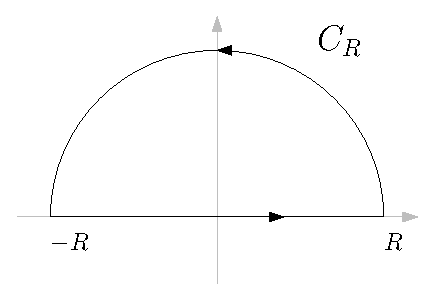
\includegraphics[scale=1]{circ.eps}
    \caption{Полукруг в верхней полуплоскости с обходом против часовой стрелки}
		\label{fig:13.1}
\end{figure}
\\
Пусть 
\begin{align*}
  & I_R = \int_{\gamma_R}f(z)dz = 2 \pi i \left( \us{z_0}{\res} f(z) +  \us{z_1}{\res} f(z)\right) = 2 \pi i \left( \left.\frac{1+z^2}{4z^3}\right|_{z_0} + \left.\frac{1+z^2}{4z^3}\right|_{z_1}\right) = 2 \pi i \cdot \\
  & \cdot \left( \frac{1+\exp\left( \frac{2i \pi}{4} \right)}{4 \exp \left( \frac{3i \pi}{4} \right)} +  \frac{1+\exp\left( \frac{6i \pi}{4} \right)}{4 \exp \left( \frac{9i \pi}{4} \right)}\right) = 2 \pi i \left( \frac{\exp\left( \frac{-i\pi}{4} \right) + \exp\left( \frac{i\pi}{4} \right)}{2 i \cdot 2} +  \frac{\exp\left( \frac{-3i\pi}{4} \right) + \exp\left( \frac{3i\pi}{4} \right)}{-2 i \cdot 2}\right) = \\
  & = \pi \left( \cos \frac{\pi}{4} - \cos \frac{3\pi}{4} \right) = \pi \sqrt{2}
\end{align*}
\begin{align*}
  & \pi \sqrt{2} = \int_{-R}^{+R}f(z) + \int_{C_R}f(z) \us{R\to \infty}{\longrightarrow} \int_{-\infty}^{+\infty} f(z) = \int_{-\infty}^{\infty}f(x)
\end{align*}
Итак, достаточно доказать
\begin{align*}
  & \int_{C_R}f(z)  \us{R\to \infty}{\longrightarrow} 0
\end{align*}
чтобы получить, что $I = \pi \sqrt{2}$.
    \begin{flushright}
    \textit{Лекция 10 (от 06.10)}
\end{flushright}
\section{$\S 14.$ Приращение аргумента $z$ вдоль кривой}

    \begin{flushright}
    \textit{Лекция 11 (от 12.10)}
\end{flushright}
\Def
Пусть в области $G$ задано семейство гладких кривых $\left\{ \gamma_\alpha
\right\}$, $\alpha \in [a,b]$, заданных при помощи параметра $t$: $z(t,
\alpha)$, $t \in [0;1]$. Если $z(t, \alpha)$ и $z'_t(t, \alpha)$ непрерывны на
$[0;1] \times [a,b]$, то говорят, что в области $G$ $\gamma_{\alpha}$
\textbf{задает непрерывную деформацию кривой $\gamma_a$ в кривую $\gamma_b$}.
\\
Если $\forall \alpha \in [a;b] \ z(0, \alpha) = z_0, \ z(1, \alpha) = z_1$, то
это называют \textbf{гомотетией $\gamma_a$ в $\gamma_b$}.
\theorem
Пусть в $\CC \setminus \{0\}$ задана непрерывная деформация $\gamma_a$ в
$\gamma_b$ через семейство $\left\{ \gamma_\alpha \right\}_{\alpha \in [a;b]}$.
Пусть $\exists A \in \CC, \ A \neq 0$ такое, что $\forall \alpha \in [a;b] \
z(1,\alpha) = Az(0, \alpha)$ и $I(\alpha) = \Delta_{\gamma_\alpha}\argt z =
\Delta_{[0;1]}\argt z(t, \alpha)$. Тогда $\forall \alpha \in [a,b] \ I(\alpha) =
const$. В частности, $\Delta_{\gamma_a}\argt z = \Delta_{\gamma_b}\argt z$.
\pr
По теореме $14.1$ $\forall \alpha \in [a;b] \ \exists \varphi(t, \alpha)$,
непрерывная по $t \in [0;1]$. $\varphi(t, \alpha) \in \Arg z (t, \alpha)$.
\begin{align*}
  & I(\alpha) = \Delta_{\gamma_\alpha}\argt z = \varphi(1, \alpha) - \varphi(0, \alpha) \in \Arg \frac{z(1, \alpha)}{z(0, \alpha)}
\end{align*}
\begin{align*}
  & \frac{z(1, \alpha)}{z(0, \alpha)} = A \neq 0 \Rightarrow \forall \psi_0 \in \Arg A \hookrightarrow I(\alpha) = \psi_0+2\pi k(\alpha), \ k(\alpha) \in \ZZ
\end{align*}
Значит, $I(\alpha)$ ступенчатая; но по определению приращения аргумента через
интеграл она непрерывна. Значит, она постоянна.
\\
$\forall z(t) \in C[0;1]$ таких, что $\forall t \in [0;1] \ z(t) \neq 0$ и $r =
\dst \min_{t \in [0;1]} \left| z(t) \right|$ положим $\varepsilon\in \left( 0;
    \dst \frac{r}{2} \right)$. Тогда существует \textbf{гладкая
  $\varepsilon$-аппроксимация $z(t)$}: $\forall t \in [0;1] \ z_\varepsilon(t)
\neq 0$, $\left| z(t) - z_\varepsilon(t) \right| \leq \varepsilon$,
$z_\varepsilon(0) = z(0)$, $z_\varepsilon(1) = z(1)$.
\\
Докажем это, построив пример. Действительно, по теореме Вейерштрасса
\begin{align*}
  & \exists P_n(t): \ \forall t \in [0;1] \left| z(t) - P_n(t) \right| < \frac{\varepsilon}{2}
\end{align*}
Положим
\begin{align*}
  & z_\varepsilon(t) = P_n(t) + \left( z(0)-P_n(0) \right)\left( 1-t \right) + \left( z(1)-P_n(1) \right)t
\end{align*}
Для такой функции выполняется $z(0) = z_\varepsilon(0)$, $z(1) =
z_\varepsilon(1)$; также
\begin{align*}
  & \abs{z(t) - z_\varepsilon(t)} \leq \abs{z(t) - P_n(t)} + \left| z(0)-P_n(0) \right| \left( 1-t \right) + \left| z(1)-P_n(1) \right|t < \frac{\varepsilon}{2} + \frac{\varepsilon}{2}(1-t) + \frac{\varepsilon}{2}(t) = \varepsilon
\end{align*}
и, наконец,
\begin{align*}
  & \abs{z_\varepsilon(t)} \geq \left| z(t) \right| - \left| z(t) - z_\varepsilon(t) \right| \geq r - \varepsilon \geq \frac{r}{2} > 0
\end{align*}
\Def
\textbf{Приращением аргумента непрерывной функции $z(t)$ вдоль непрерывной
  кривой $\gamma$ на $[0;1]$} называется $\Delta_{[0,1]}\argt z(t) =
\Delta_{[0,1]}\argt z_\varepsilon(t)$ для любой $\varepsilon$-аппроксимации
$z(t)$ при малых $\varepsilon$ ($\varepsilon \in \left( 0, \dst \frac{r}{2}
\right)$).
\prop
Определение $[14.4]$ не зависит от выбора $z_\varepsilon$.
\pr
Пусть $z_\varepsilon$~--- гладкая $\varepsilon$-аппроксимация,
$\tilde{z}_\varepsilon$~--- другая гладкая $\varepsilon$-аппорксимация.
Тогда
\begin{align*}
  & z(t, \alpha) = \alpha z_\varepsilon(t) + (1-\alpha)\tilde{z}_\varepsilon(t), \ \alpha \in [0;1], \ t \in [0;1]
\end{align*}
\begin{align*}
  & \abs{z(t, \alpha)} \geq \left| z(t) \right| - \left| z(t, \alpha) - z(t) \right| > r - \varepsilon \geq \frac{r}{2} > 0
\end{align*}
Значит, задана непрерывная деформация, и по теореме $14.3$ получаем, что
\begin{align*}
  & \Delta_{[0;1]}\argt z_\varepsilon(t) = \Delta_{[0;1]}\argt \tilde{z}_\varepsilon(t)
\end{align*}
\corollary
Пусть $\os{\circ}{\gamma}$~--- замкнутая непрерывная кривая, $0 \not \in
\os{\circ}{\gamma}$; тогда $\exists k(\os{\circ}{\gamma})\in \ZZ$:
$\Delta_{\os{\circ}{\gamma}}\argt z = 2 \pi k(\os{\circ}{\gamma})$.
\section{$\S 15.$ Регулярные ветви многозначных функций $\{\sqrt[n]{z}\}$ и $\Ln
  z$.}
Определим на $\CC\setminus\{0\}$:
\begin{equation}\label{(15.1)}
    \left\{ \sqrt[n]{z} \right\} = \sqrt[n]{\left| z \right|}\exp\left( \frac{i}{n} \Arg z \right)
\end{equation}
\begin{equation}\label{(15.2)}
    \left\{ \Ln z \right\} = \ln\left| z \right| + i \Arg z
\end{equation}
\begin{equation}\label{(15.3)}
    \Arg z= \left\{ \argt z + 2 \pi k \mid k \in \ZZ \right\}
\end{equation}
Из теоремы $2 \ \S 5$ (следствия $1$) можем видеть, что на $\CC \setminus \left(
    -\infty; 0 \right]$ существуют регулярные ветви:
\begin{equation}\label{(15.4)}
    \begin{split}
        & g_0(z) = \sqrt[n]{\left| z \right|}\exp\left( \frac{i}{n} \argm z \right) \\
        & h_0(z) = \ln\left| z \right| + i \argm z \\
        & \argm z \in \left( -\pi; \pi \right)
    \end{split}
\end{equation}
Это \textbf{главные регулярные ветви $\left\{\sqrt[n]{z}\right\}$ и $\Ln z$}.
\\
Рассмотрим \textbf{простейший случай}.
\\
Фиксируем $\varphi_0 \in \left( -\pi; \pi \right)$, $n \geq 2$.
\\
Пусть область
\begin{align*}
  & G_{1, \varphi_0} = \left\{ z \neq 0 \mid z = re^{i\varphi}, \ r > 0, \ \varphi \in \left( \frac{\varphi_0}{n}; \frac{\varphi_0 + 2\pi}{n} \right) \right\}
\end{align*}
$w = z^n$ однолистна на $G_{1, \varphi_0} \mapsto \CC \setminus
\lambda_{\varphi_0}$, гле $\lambda_{\varphi_0} = \left\{ z \mid z = re^{i
      \varphi_0}, \ r> 0\right\}\cup \{0\}$
\\
По следствию $1$ $\S 5$
\begin{equation}\label{(15.5)}
    \begin{split}
        & g_*(z) = \sqrt[n]{\left| z \right|}\exp\left( \frac{i}{n} \arg_* z \right) \\
        & \arg_* z \in \left( \varphi_0; \varphi_0+2\pi \right)
    \end{split}
\end{equation}
дает регулярную ветвь.
Пусть область
\begin{align*}
  & G_{2, \varphi_0} = \left\{ z \mid \Img z \in \left( \varphi_0; \varphi_0 + 2\pi \right) \right\}
\end{align*}
$w = e^z$ однолистна на $G_{2, \varphi_0}$, и
\begin{equation}\label{(15.6)}
    \begin{split}
        & h_*(z) = \ln\left| z \right| + i \arg_* z \\
        & \arg_* z \in \left( \varphi_0; \varphi_0+2\pi \right)
    \end{split}
\end{equation}
дает регулярную ветвь.
\lemma
Пусть $G$~--- область в $\CC \setminus \lambda_{\varphi_0}$. Тогда все
непрерывные ветви $\left\{ \sqrt[n]{z} \right\}$ и $\Ln z$ в $G$ являются
регулярными и удовлетворяют соотношениям:
\begin{equation}\label{(15.7)}
    g_k(z) = g_*(z) \exp\left( \frac{i}{n} 2 \pi k\right), \ k \in \{0, \dots, n-1\}
\end{equation}
\begin{equation}\label{(15.8)}
    h_k(z) = h_*(z) + 2i \pi k, \ k \in \ZZ
\end{equation}
\pr
Пусть $g(z)$~--- непрерывная ветвь $\left\{\sqrt[n]{z}\right\}$ в $G$; $g^n(z) \equiv
    z$, $g_*^n(z) \equiv z$. Деля,
    \begin{align*}
      & \left( \frac{g^n(z)}{g_*^n(z)} \right)^n = 1 \Rightarrow \frac{g(z)}{g_*(z)} \in \left\{ \sqrt[n]{1} \right\} = \exp \left( \frac{i}{n} 2 \pi k(z) \right), \ k(z) \in \left\{ 0, \dots, n-1 \right\}
    \end{align*}
В левой части функция непрерывная, в правой~--- ступенчатая, а значит, $k(z) =
k_* = const$, откуда видно, что $g(z)$ удовлетворяет \eqref{(15.7)}.
\\
Пусть $h(z)$~--- непрерывная ветвь $\Ln z$ в $G$; $e^{h(z)} \equiv z$,
$e^{h_*(z)} \equiv z$. Деля,
\begin{align*}
  & e^{h(z)-h_*(z)} = 1 \Rightarrow h(z) - h_*(z) = 2i\pi k(z)
\end{align*}
Значит, $k(z) = k_* = const$, откуда видно, что $h(z)$ удовлетворяет
\eqref{(15.8)}.
\lemma
В любом кольце $K_{r,R}(0) = \left\{ z \mid r < \left| z \right| < R \leq
    +\infty \right\}$ нет непрерывных ветвей $\left\{ \sqrt[n]{z} \right\}$ или
$\Ln z$.
\pr
Предположим противное: $\exists K_{r, R}(0)$: $\left\{ \sqrt[n]{z} \right\}$
имеет в нем непрерывную ветвь $g(z)$. 
\\
Тогда рассмотрим область $G = K \setminus \left( -\infty;0 \right]\subseteq \CC
\setminus \left( -\infty; 0 \right]$. Эта область удовлетворяет условиям леммы
$1$, но по этой лемме $\exists k_* \in \left\{ 0, \dots, n-1 \right\}$: $g(z) =
g_0(z)\exp \left( \dst \frac{i}{n} 2 \pi k_* \right)$, $z \in G$. Заметим, что
$\forall x \in \left( -R;-r \right)$
\begin{align*}
& g(x+i0) = \sqrt[n]{\left| z \right|}\exp \left( \frac{i \pi}{n} + \frac{2 i \pi k_*}{n}\right) \\
& g(x-i0) = \sqrt[n]{\left| z \right|}\exp \left( \frac{-i \pi}{n} + \frac{2 i \pi k_*}{n}\right) \\
\end{align*}
Они не равны, противоречие с предположением о непрерывности.
\\
Аналогично можно провести доказательство для $\Ln z$.
\corollary
Если $0 \in G$ или $\infty \in G$, то в $G$ не существует непрерывной ветви
$\left\{ \sqrt[n]{z} \right\}$ или $\Ln z$.
\\
Рассмотрим \textbf{общий случай}.
\\
Пусть $G \subseteq \CC$~--- односвязая область, $0 \not \in G$.
\lemma
В односвязной области $G$, $0 \not \in G$ существуют непрерывные ветви $\Arg z$.
\pr
Фиксируем $z_0 \in G$, $\psi_0 \in \Arg z_0$.
\\
Пусть $\gamma_{z_0z}$~--- гладкая кривая из $z_0$ в $z$, $ \gamma \subseteq G$.
Пусть
\begin{align*}
  & \varphi_{\gamma_{z_0z}} = \psi_0 + \Delta_{\gamma_{z_0z}}\argt z
\end{align*}
\begin{align*}
  & \varphi_{\gamma_{z_0z}} \in \Arg z
\end{align*}
\begin{align*}
  & \Delta_{\gamma_{z_0z}}\argt z = \Img \int_{\gamma_{z_0z}}\frac{d \zeta}{\zeta}
\end{align*}
Знаем, что $\dst \frac{1}{z}$ регулярна в $G$, а значит, по теореме Коши
\begin{align*}
  & \forall \os{\circ}{\gamma} \subseteq G \ \int_{\os{\circ}{\gamma}}\frac{d\zeta}{\zeta} = 0
\end{align*}
Тогда
\begin{align*}
  & \Phi(z) = \int_{\gamma_{z_0z}}\frac{d \zeta}{\zeta}
\end{align*}
регулярна в $G$;
\begin{equation}\label{(15.9)}
    \varphi_{\gamma_{z_0z}} = \varphi_0(z) = \psi_0 + \Delta_{\gamma_{z_0z}}\argt z \in \Arg z
\end{equation}
будет непрерывной, и, зная это, легко построить
\begin{equation}\label{(15.10)}
    \tilde{g}(z) = \sqrt[n]{\left| z \right|} \exp\left( \frac{i}{n} \varphi_0(z) \right)
\end{equation}
\begin{equation}\label{(15.11)}
    \tilde{h}(z) = \ln \left| z \right| + i \varphi_0(z)
\end{equation}
Это непрерывные ветви $\left\{ \sqrt[n]{z} \right\}$ и $\Ln z$ соответственно в
$G$.
\theorem
В односвязной $G$, $0 \not \in G$ существуют непрерывные ветви $\left\{
    \sqrt[n]{z} \right\}$ и $\Ln z$, являющиея регулярными ветвями и
удовлетворяюшщие соотношениям:
\begin{equation}\label{(15.12)}
    \tilde{g}_k(z) = \tilde{g}(z)\exp\left( \frac{2i\pi k}{n} \right), \ k \in \left\{ 0, \dots, n-1 \right\}
\end{equation}
\begin{equation}\label{(15.13)}
    \tilde{h}_k(z) = \tilde{h}(z) + 2 i \pi k, \ k \in \ZZ
\end{equation}
\pr
Всякая ветвь такова по лемме $1$. Докажем регулярность $\tilde{g}(z)$.
\\
Рассмотрим $z_1 \in G$: $\exists B_r(z_1) \subseteq G$, $0 \not \in B_r(z_1)$
$\Rightarrow$ $\exists \varphi_0 \in [-\pi, \pi): \ B_r(z_1) \subseteq \CC
\setminus \lambda_{\varphi_0}$.
\\
Значит, по лемме $1$ $\tilde{g}(z)$ регулярна в $B_r(z_1)$, а значит, и в $z_1$;
в силу произвольности выбора $z_1$ можем сказать, что функция регулярна в $G$.
\\
Аналогично можем провести доказательство для $\tilde{h}(z)$.

    \begin{flushright}
    \textit{Лекция 12 (от 13.10)}
\end{flushright}
\corollary
Пусть $G$ односвязна, $0 \not \in G$. Тогда для регулярной $h_k \in \Ln z$
справедлива формула Ньютона-Лейбница
\begin{equation}\label{(15.14)}
    h_k(z) = h_k(a) + \int_{\gamma_{az}}\frac{d\zeta}{\zeta}
\end{equation}
где $a \in G$, $\gamma_{az} \subseteq G$.
\pr
\begin{align*}
  & h_k(z) = h_0(z) + 2i \pi k
\end{align*}
\begin{align*}
  & h_0(z) = \ln \left| z \right| + i \left( \psi_0 + \Delta_{\gamma_{az}}\argt z \right)
\end{align*}
\begin{align*}
  & \Real \int_{\gamma_{az}} \frac{d\zeta}{\zeta} = \ln \left| z \right| - \ln \left| a \right|
\end{align*}
Действительно, пусть $z(t) = \gamma_{az}$, тогда
\begin{align*}
  & \Real \int_{\gamma_{az}} \frac{d\zeta}{\zeta} = \Real \int_0^1 \frac{xx'+yy'}{x^2+y^2} d \tau = \Real \int_0^1 \frac{d \sqrt{x^2+y^2}}{\sqrt{x^2+y^2}} = \ln \left| z(1) \right| - \ln \left| z(0) \right| = \ln \left| z \right| - \ln \left| a \right|
\end{align*}
\begin{align*}
  & h_k(z) = \ln \left| z \right| - \ln \left| a \right| + \ln\left| a \right| + i \left( \psi_0 + 2 \pi k \right) + i \Delta_{\gamma_{az}}\argt z = h_k(a) + \int_{\gamma_{az}}\frac{d\zeta}{\zeta}
\end{align*}
\section{$\S 16$. Регулярные ветви $\{\sqrt[n]{f(z)}\}$ и $\Ln f(z)$.}
\sug
$G$~--- область, $f$ регулярна на $G$, $\forall z \in G \ f(z) \neq 0$.
\begin{equation}\label{(16.1)}
    \left\{ \sqrt[n]{f(z)} \right\} = \sqrt[n]{\left| f(z) \right|} \exp \left( \frac{i}{n}\Arg f(z) \right)
\end{equation}
\begin{equation}\label{(16.2)}
    \Ln f(z) = \ln \left| f(z) \right| +i \Arg f(z)
\end{equation}
\begin{equation}\label{(16.3)}
    \Arg f(z) = \left\{ \argt f(z) + 2 \pi k \mid k \in \ZZ \right\}
\end{equation}
\Def
Пусть $\gamma$~--- непрерывная кривая в $G$, $f$ удовлетворяет предположению
$1$. Пусть $z(t)$~--- параметризация $\gamma$, $t \in [0;1]$. Пусть $\Gamma =
f(\gamma): \ w = f(z(t)), \ t \in [0;1]$. Тогда \textbf{приращением аргумента
  $f(z)$ вдоль кривой $\gamma$} называется
\begin{equation}\label{(16.4)}
    \Delta_{\gamma}\argt f(z) = \Delta_\Gamma\argt w = \Delta_{[0;1]}\argt f(z(t))
\end{equation}
\lemma
Пусть $f$, $f_1$, $f_2$ удовлетворяют предположению $1$ в области $G$. Тогда
\begin{enumerate}
    \item для любой непрерывной $\gamma \subseteq G$ выполняется логарифмическое
    свойство:
    \begin{equation}\label{(16.5)}
        \Delta_{\gamma}\argt (f_1f_2) = \Delta_\gamma\argt f_1 + \Delta_{\gamma}\argt f_2
    \end{equation}
    \item если $\gamma \subseteq G$ разбита точкой $A \in \gamma$ на части
    $\gamma_1$, $\gamma_2$, то
    \begin{equation}\label{(16.6)}
        \Delta_{\gamma}\argt f = \Delta_{\gamma_1}\argt f + \Delta_{\gamma_2}\argt f
    \end{equation}
    \item если $\gamma$~--- кусочно гладкая кривая в $G$, то
    \begin{equation}\label{(16.7)}
        \Delta_{\gamma}\argt f(z) = \Img \int_\Gamma \frac{dw}{w} = \Img \int_{\gamma} \frac{f'(\zeta)}{f(\zeta)}d\zeta
    \end{equation}
\end{enumerate}
\pr
Утверждения леммы очевидны из определения приращения аргумента функции.
\lemma
Пусть $G$ односвязна, $\os{\circ}{\gamma} \subseteq G$ замкнута и непрерывна.
Пусть $f$ удовлетворяет предположению $1$. Тогда
\begin{equation}\label{(16.8)}
    \Delta_{\os{\circ}{\gamma}}\argt f(z) = 0
\end{equation}
\pr
Пусть $\os {\circ}{\gamma} \subseteq G$ гладкая и замкнутая, параметризованная
$z(t)$.
\\
$\forall z_0 \in \os{\circ}{\gamma}$ существует непрерывная деформация $z(t,
\alpha)$ такая, что $z(t,a) = z(t)$, $z(t,b) = z_0$. По теореме $3$ $\S 14$
$I(\alpha) = const$, а значит,
\begin{align*}
  \Delta_{[0;1]}\argt f(z) = \Delta_{[0;1]}\argt f(z_0) = 0
\end{align*}
\lemma
Пусть $f$ удовлетворяет предположению $1$ в области $G$. Если в области $G$
сществуют регулярные ветви $h_0(z)$ или $g_0(z)$~--- регулярные ветви $\Ln f(z)$
или $\left\{ \sqrt[n]{f(z)} \right\}$, то все их непрерывные ветви регулярны и
удовлетворяют соотношениям:
\begin{equation}\label{(16.9)}
    h_k(z) = h_0(z) + 2i \pi k, \ k \in \ZZ
\end{equation}
\begin{equation}\label{(16.10)}
    g_k(z) = g_0(z) \exp\left( \frac{i}{n} 2 \pi k\right), \ k \in \{0, \dots, n-1\}
\end{equation}
\pr
Доказательство полностью аналогично доказательству леммы $15.1$.
\lemma
Пусть $f$ удовлетворяет предположению $1$ в $G$. Если в $G$ существует
регулярная ветвь $h(z)$ многозначной функции $\Ln z$, то $\forall a,b \in G$
\begin{equation}\label{(16.11)}
    h(b) = h(a) + \ln \left| \frac{f(b)}{f(a)} \right| + i \Delta_{\gamma_{ab}}\argt f(z)
\end{equation}
\pr
\begin{align*}
  & h(z) = \ln \left| f(z) \right| + i \Img h(z)
\end{align*}
В силу регулярности $h$ $\Img h$ будет гармонической функцией от $x, y$. Значит,
\begin{align*}
  & \varphi(z) = \Img h(z) \in \Arg f(z)
\end{align*}
Пусть $a \in G$, $\psi_0 \in \Arg f(a)$, $h(a) = \ln \left| f(a) \right| + i
\psi_0$. Пусть $\gamma_{az}$~--- гладкая кривая с параметризацией $z(t)$, $t \in
[0;1]$, $\varphi(z(t))$~--- гладкая ветвь $\Arg f(z(t))$.
\begin{align*}
  & \Delta_{\gamma_{az}}\argt f(z) = \varphi(z(t))-\varphi(z(0)) = \Img h(z) - \Img h(a)
\end{align*}
\begin{align*}
  & h(b) = \ln \left| f(b) \right| + i \Img h(b)
\end{align*}
\begin{align*}
  & h(a) = \ln \left| f(a) \right| + i \Img h(a)
\end{align*}
\begin{align*}
  & h(b) - h(a) = \ln \left| \frac{f(b)}{f(a)} \right| + i \left( \Img h(b) - \Img h(a) \right)
\end{align*}
Отсюда следует \eqref{(16.11)}.
\theorem
Пусть $f$ удовлетворяет предположению $1$ в $G$. Тогда у  $\Ln f(z)$ существуют
регулярные ветви в $G$ тогда и только тогда, когда выполняется \eqref{(16.8)}
для любой замкнутой $\os{\circ}{\gamma}\subseteq G$.
\pr
Докажем в обе стороны.
\begin{itemize}
    \item Необходимость.
    \\
    Если есть регулярные ветви $h(z) \in \Ln z$  $G$, то из \eqref{(16.11)} при
    $a = b$ получаем \eqref{(16.8)}.
    \item Достаточность.
    \\
    Пусть выполнено \eqref{(16.8)}. Фиксируем $a \in G$, $h(a) \in \Ln f(a)$.
    Рассмотрим
    \begin{equation}\label{(16.12)}
        h(z) = h(a) + \ln \left| \frac{f(z)}{f(a)} \right| + i \Delta_{\gamma_{az}}\argt f(z)
    \end{equation}
    В действительности приращение аргумента может зависеть от $\gamma$, поэтому
    корректнее расссматривать это как $h(\gamma_{az})$.
    \\
    По \eqref{(16.8)}
    \begin{align*}
      & \Delta_{\gamma_{az}}\argt f(z) = \Delta_{\tilde{\gamma}_{az}}\argt f(z)
    \end{align*}
    \begin{align*}
      & \os{\circ}{\gamma} = \gamma_{az}+\tilde{\gamma}^{-1}_{az}
    \end{align*}
    Значит, $h(z)$~--- функция лишь точки $z$.
    \begin{equation}\label{(16.13)}
        \exists \psi_0 \in \Arg f(a): \ h(a) = \ln \left| f(a) \right| + i \psi_0
    \end{equation}
    Из \eqref{(16.12)} следует, что
    \begin{align*}
      & h(z) = \ln \left| f(z) \right| + i \left( \psi_0 + \Delta_{\gamma_{az}}\argt f(z) \right) \in \Ln f(z)
    \end{align*}
    \begin{align*}
      & \Real \int_{\gamma_{az}}\frac{f'(\zeta)}{f(\zeta)}d\zeta = \ln \left| f(z) \right| - \ln \left| f(a) \right|
    \end{align*}
    \begin{align*}
      & \Delta_{\gamma_{az}}\argt f(z) = \Img \int_{\gamma_{az}}\frac{f'(\zeta)}{f(\zeta)}d\zeta
    \end{align*}
    Отсюда следует, что
    \begin{align*}
      & h(z) = \ln \left| f(a) \right| + \ln \left| f(z) \right| - \ln \left| f(a) \right| + i \Delta_{\gamma_{az}} \argt f(z) + i \psi_0 = \ln \left| f(a) \right| + \int_{\gamma_{az}}\frac{f'(\zeta)}{f(\zeta)}d \zeta +  i \psi_0 
    \end{align*}
    Функция
    \begin{align*}
      & \varphi(z) = \int_{\gamma_{az}}\frac{f'(\zeta)}{f(\zeta)}d\zeta
    \end{align*}
    регулярна по теореме $3$ $\S 6$, а значит, и $h(z)$ регулярна.
\end{itemize}
\lemma
Пусть $f$ удовлетворяет предположению $1$ в $G$, $n \in \NN$, $n \geq 2$. Если в
$G$ существует регулярная ветвь $g(z)$ многозначной функции $\left\{
    \sqrt[n]{f(z)} \right\}$, то $\forall a, b \in G$
\begin{equation}\label{(16.14)}
    g(b) = g(a) \sqrt[n]{\left| \frac{f(b)}{f(a)} \right|}\exp \left( \frac{1}{n}\Delta_{\gamma_{ab}}\argt f(z) \right)
\end{equation}
\pr Доказательство разбиваем на два этапа.
\begin{enumerate}
    \item Пусть для начала $G$ односвязна.
    \\
    По лемме $2$ $\forall \os{\circ}{\gamma} \subseteq G$ выполняется
    \eqref{(16.8)} и тогда, по лемме $4$:
    \begin{align*}
      & \exists h(z) = h(a) + \ln \left|\frac{f(z)}{f(a)}\right|+ i\left(\Delta_{\gamma_{az}}\argt f(z)\right) \in \Ln f(z)
    \end{align*}
    регулярные ветви.
    \begin{align*}
      & g_0(z) = \exp \left(\frac{i}{n} h(z)\right)
    \end{align*}
    \begin{align*}
      & \exists \psi_0 \in \Arg f(a): \ h(z) = \ln \left| f(z) \right| + i \left( \psi_0 + \Delta_{\gamma_{az}}\argt f(z) \right)
    \end{align*}
    Тогда
    \begin{align*}
      & g_0(z) = \sqrt[n]{\left| f(z) \right|}\exp \left( \frac{i}{n} \left( \psi_0 + \Delta_{\gamma_{az}}\argt f(z) \right) \right)\in \left\{ \sqrt[n]{f(z)} \right\}
    \end{align*}
    регулярная ветвь.
    \\
    По лемме $3$ $\exists k \in \left\{ 0, \dots, n-1 \right\}: \ g(z) = g_0(z)$.
    Отсюда следует \eqref{(16.14)}.
    \item $G$~--- область.
    \begin{align*}
      &\forall a, b \in G, \ \forall \gamma_{ab} \subseteq G
    \end{align*}
    можем выбрать такие $a=z_0, z_1, \dots, z_{K-1}, z_K = b \in \gamma_{ab}$,
    что $\left| z_k - z_{k-1} \right|< l_k$, где $l_k$~--- расстояние до
    границы.
    \begin{align*}
      & \exists \left\{ B_\varepsilon(z_k) \right\}_{k=0}^K \subseteq G: \ z_{k+1} \in B_{\varepsilon}(z_k)
    \end{align*}
    Каждый из $B_{\varepsilon}(z_k)$ односвязен, поэтому выполняется
    \eqref{(16.14)}:
    \begin{align*}
      & \forall k \in \left\{ 0, \dots, K-1 \right\} \ \frac{g(z_{k+1})}{g(z_k)} = \sqrt[n]{\frac{f(z_{k+1})}{f(z_k)}} \exp \left( \frac{i}{n} \Delta_{\gamma_{z_kz_{k+1}}}\argt f(z) \right)
    \end{align*}
    Перемножая по всем $k$, получаем
    \begin{align*}
      & \frac{g(b)}{g(a)} = \sqrt[n]{\left| \frac{f(b)}{f(a)} \right|}\exp \left( \frac{i}{n} \sum_{k=0}^{K-1} \Delta_{\gamma_{z_kz_{k+1}}} \argt f(z) \right) = \sqrt[n]{\frac{\left| f(b) \right|}{\left| f(a) \right|}}\exp \left( \frac{i}{n}\Delta_{\gamma_{ab}}\argt f(z) \right)
    \end{align*}
    Это ни что иное, как \eqref{(16.14)}.
\end{enumerate}\theorem
Пусть $f$ удовлетворяет условиям предположения $1$ в $G$. Тогда существуют
регуляртые ветви $\left\{ \sqrt[n]{f(z)} \right\}$тогда и только тогда, когда
\begin{equation}\label{(16.15)}
    \forall \os{\circ}{\gamma} \subseteq G \ \exists k(\os{\circ}{\gamma}) \in \ZZ: \ \Delta_{\os{\circ}{\gamma}}\argt f(z) = 2\pi n k(\os{\circ}{\gamma}))
\end{equation}
    \begin{flushright}
    \textit{Лекция 13 (от 19.10)}
\end{flushright}
\pr
Из леммы $5$ очевидно следует необходимость (возьмем $a = b$).
\\
Докажем достаточность. Пусть $a \in G$, $z \in G$, $\gamma_{az}\in G$, $g(a) \in
\left\{ \sqrt[n]{f(z)} \right\}$. Тогда выполняется
\begin{equation}\label{(16.16)}
    g(z) = g(a) \sqrt[n]{\left| \frac{f(b)}{f(a)} \right|}\exp \left( \frac{i}{n} \Delta_{\gamma_{az}}\arg f(z) \right)
\end{equation}
Докажем регулярность такой ветви.
\\
Для замкнутых кривых экспонента примет значение $1$, а значит, $g(z)$ зависит
только от точки $z$. Очевидно, $\forall z \in G \ g(z)\in \left\{ \sqrt[n]{f(z)}
\right\}$. Докажем ее регулярность.
\\
Фиксируем произвольную $z_1 \in G$; тогда $\exists B_\varepsilon(z_1) \subseteq G$
такой, что
\begin{equation}\label{(16.17)}
    \forall z \in B_\varepsilon(z_1) \ g(z) = g(z_1) \sqrt[n]{\left| \frac{f(z)}{f(z_1)} \right|}\exp \left( \frac{i}{n} \Delta_{\gamma_{z_1z}}\argt f(z) \right)
\end{equation}
$B_{\varepsilon}(z_1)$ односвязна, значит, по лемме $2$
$\Delta_{\os{\circ}{\gamma}}\argt f(z) = 0$ для любой замкнутой
$\os{\circ}{\gamma} \subseteq B_\varepsilon(z_1)$. Но
\begin{align*}
  & g(z) = \exp \left( \frac{i}{n} h(z) \right)
\end{align*}
\begin{align*}
  & h(z) = \ln \left| f(z) \right| + i \left(\psi_0 + \Delta_{\gamma_{z_1z}}\argt f(z)\right), \ \psi_0 \in \Arg f(z_1)
\end{align*}
\begin{equation}\label{(16.18)}
    g(z_1) = \sqrt[n]{\abs{f(z_1)}} \exp\left( \frac{i}{n}\psi_0 \right)
\end{equation}
В $B_\varepsilon(z_1)$ есть регулярная ветвь $\Ln f(z)$, причем $h(z)$~--- та
самая ветвь, значит, $g(z)$ регулярна в $B_\varepsilon(z_1)$.
\\
В силу произвольности выбора $z_1$ показали регулярность во всей $G$.
\corollary
Если $h(z)$, $g(z)$~--- регулярные ветви $\Ln f(z)$ и $\left\{ \sqrt[n]{f(z)}
\right\}$ соответственно в $G$, то
\begin{equation}\label{(16.19)}
    h'(z) = \frac{f'(z)}{f(z)}
\end{equation}
\begin{equation}\label{(16.20)}
    g'(z) = \frac{f'(z)}{n\left( g(z) \right)^{n-1}}
\end{equation}
\pr
\begin{align*}
  & e^{h(z)} \equiv f(z) \rightarrow h'(z)e^{h(z)} \equiv f'(z) \Rightarrow h'(z) \equiv \frac{f'(z)}{f(z)}
\end{align*}
\begin{align*}
  & (g(z))^n \equiv f(z) \Rightarrow n(g(z))^{n-1}g'(z) \equiv f'(z) \Rightarrow g'(z) = \frac{f'(z)}{n\left( g(z) \right)^{n-1}}
\end{align*}
\section{$\S 17.$ Примеры вычисления регулярных ветвей.}
\Example
\begin{align*}
  & \left\{ \sqrt[4]{z^3(z+1)} \right\}, \ G = \CC \setminus[-1;0]
\end{align*}
Если ветвь существует, то
\begin{align*}
  & g_1(2) = i \sqrt[4]{24}
\end{align*}
При этих условиях найти $g_1(i)$, $g'_1(i)$.
\nonum
Заметим: $f(z) = z^3(z+1)$, $n=4$. Видим, что в $G$ $f(z) \neq 0$.
\\
$\forall \os{\circ}{\gamma} \subseteq G$~--- замкнутой~--- рассмотрим
$\Delta_{\os{\circ}{\gamma}}\argt f(z)$.
\begin{align*}
  & \Delta_{\os{\circ}{\gamma}}\argt f(z) = \Delta_{\os{\circ}{\gamma}}\argt z^3(z+1) = 3 \Delta_{\os{\circ}{\gamma}}\argt z + \Delta_{\os{\circ}{\gamma}}\argt (z-1)
\end{align*}
\begin{figure}[h!]
		\centering
		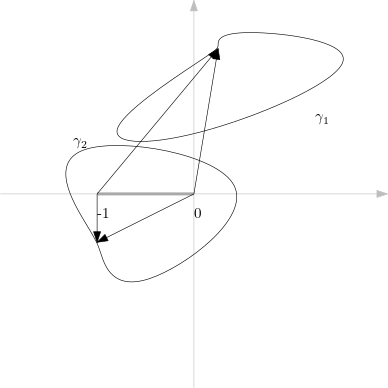
\includegraphics[scale=0.5]{Ex1.png}
		\label{fig:17.1}
\end{figure}
На кривых вида $\gamma_1$ (не опоясывающих разрез) приращение обоих аргументов
равно нулю (а значит, и суммарное), а на кривых вида $\gamma_2$ приращение
аргумента составит $8 \pi$. Оба случая удовлетворяют условию существования
регулярных ветвей.
\\
Докажем строго. Пусть $\os{\circ}{\gamma} = z(t)$, $t \in [0;1]$, $z(0) = z(1) =
z_0 \in \gamma$, $z(t, \alpha) = z(t) - \alpha$, $\alpha \in [-1;0]$. $\forall
(t, \alpha) \ z(t, \alpha) \neq 0$, $\forall \alpha \ z(1, \alpha) = z(0,
\alpha) = z_0 - \alpha$. Значит, по теореме $3$ $\S 14$ $I(\alpha) =
\Delta_{[0;1]}\argt z(t, \alpha) = const$, т.~е.
\begin{align*}
  & \Delta_{[0;1]} \argt z(t) = \Delta_{[0;1]} \argt(z(t) + 1) = \Delta_{\os{\circ}{\gamma}}z = \Delta_{\os{\circ}{\gamma}}(z+1) = 2 \pi k(\os{\circ}{\gamma})
\end{align*}
\begin{align*}
  & \Delta_{\ogamma} \argt f(z) = 4 \Delta_{\ogamma} \argt z = 8 \pi
\end{align*}
Желаемое условие выполняется.
\\
Значит,
\begin{align*}
  & g_1(z) = g_1(2) \sqrt[4]{\frac{\left| z^3(z+1) \right|}{24}} \exp \left( \frac{i}{4}\left( \Delta_{\gamma{2z}}\argt f(z) \right) \right)
\end{align*}
\begin{align*}
  & g_1(i) = g_1(2) \sqrt[4]{\frac{\left| i^3(i+1) \right|}{24}} \exp \left( \frac{i}{4}\left( \Delta_{\gamma_{2,i}}\argt f(z) \right) \right) = 2^{\frac{1}{8}}i\exp \left( \frac{i}{4} \left( 3\Delta_{\gamma_{2,i}}\argt z + \Delta_{\gamma_{2,i}} \argt (z+1) \right) \right) = \\
  & = 2^{\frac{1}{8}}i\exp \left( \frac{i}{4} \left( 3\frac{\pi}{2} + \frac{\pi}{4} \right) \right) = 2^{\frac{1}{8}}i\exp \left( \frac{7i\pi}{16} \right) =  2^{\frac{1}{8}}e^{\frac{15i\pi}{16}}
\end{align*}
\begin{align*}
  & g_1'(z) = \frac{4z^3+3z^2}{4g_1^3(z)}
\end{align*}
\begin{align*}
  & g_1'(i) = \frac{-4i -3}{4\cdot 2^{\frac{3}{8}}e^{\frac{45i\pi}{16}}} = -(4i+3)2^{-\frac{19}{8}}e^{-\frac{13i\pi}{16}}
\end{align*}
\Example
\begin{align*}
  & \Ln (1-z^2), \ G = \CC \setminus (-\infty; 1]
\end{align*}
Если ветвь существует, то
\begin{align*}
  & \Img h\left( \frac{i}{5} \right) = 0
\end{align*}
При этих условиях найти разложение $h$ в ряд Тейлора по степеням $(z+i)$,
область, где $h(z) = S(z)$~--- сумма своего ряда Тейлора, его радиус сходимости
$R$ и $S\left( \dst \frac{i}{5} \right)$.
\nonum
$G$ односвязна. Заметим: $f(z) = 1-z^2 \neq 0$ в $G$.
\\
$\forall \gamma \subseteq G$ рассмотрим $\Delta_{\gamma}\argt f(z)$.
\begin{align*}
  & h(z) = \ln \left| z \right| + i \Img h(z)
\end{align*}
\begin{align*}
  & h\left( \frac{i}{5} \right) = \ln \frac{26}{25}
\end{align*}
\begin{figure}[h!]
		\centering
		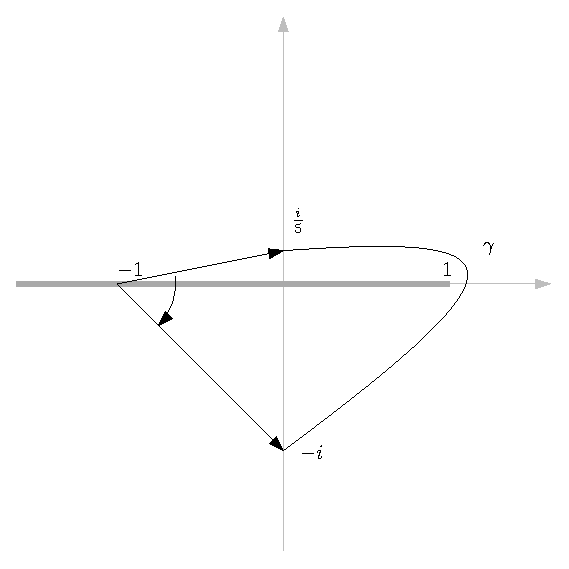
\includegraphics[scale=0.75]{Ex1.eps}
		\label{fig:17.2}
\end{figure}
\begin{align*}
  & h(-i) = \ln \frac{26}{25} + \ln \left| \frac{2}{\frac{26}{25}} \right|+ i\left( \Delta_{\gamma_{\frac{i}{5}, -i}}\argt (z+1) + \Delta_{\gamma_{\frac{i}{5}, -i}}\argt (z-1) + \Delta_{\gamma_{\frac{i}{5}, -i}}\argt (-1) \right) = \ln 2 - 2 i \pi
\end{align*}
Положим $\zeta = z+i$, $h(z) = h(\zeta - i) = \tilde{h}(\zeta)$. Тогда
$\tilde{h}(0) = h(-i) = \ln 2 - 2 i \pi$. Хотим разложить это в ряд.
\begin{align*}
  & \tilde{h}(\zeta) \in \Ln (1-(\zeta - i)^2) = \Ln(2+2i\zeta - \zeta^2) = \Ln \left(2\left( 1 - \frac{\zeta}{1-i} \right)\left( 1 - \frac{\zeta}{1+i} \right) \right) = \Ln 2 + \\
  & \Ln \left( 1 - \frac{\zeta}{1-i} \right) + \Ln \left( 1 - \frac{\zeta}{1+i} \right)
\end{align*}
Из теоремы об обратной функции
\begin{align*}
  & h^*_k(z) \in \Ln (1+z), \ \left| z \right| < 1 \Rightarrow h^*_k(z) = 2 i \pi k + \sum_{n=1}^\infty \frac{(-1)^{n+1}}{n} z^n, \ \left| z \right| < 1
\end{align*}
Рассмотрим
\begin{align*}
  & h_+(\zeta) \in \Ln \left( 1 - \frac{\zeta}{1+i} \right), \ \left| \zeta \right| < \sqrt{2}, \ h_+(0) = 0 \Rightarrow h_+(\zeta) = - \sum_{n=1}^\infty \frac{\zeta^n}{n(1+i)^n}, \ \left| \zeta \right| < \sqrt{2}
\end{align*}
\begin{align*}
  & h_-(\zeta) \in \Ln \left( 1 - \frac{\zeta}{1-i} \right), \ \left| \zeta \right| < \sqrt{2}, \ h_-(0) = 0 \Rightarrow h_-(\zeta) = - \sum_{n=1}^\infty \frac{\zeta^n}{n(1-i)^n}, \ \left| \zeta \right| < \sqrt{2}
\end{align*}
Заметим, что $\sqrt{2}$~--- максимальный радиус, т.~к. выходим на особую точку.
Видим:
\begin{align*}
  & \tilde{h}(\zeta) - h_+(\zeta) - h_-(\zeta) = \ln 2 + 2 i \pi k(\zeta)
\end{align*}
В правой части функция непрерывная, в левой ступенчатая, значит, $k = const$.
Найдем ее:
\begin{align*}
  &  \tilde{h}(0) - h_+(0) - h_-(0) = \ln 2 + 2 i \pi k = \ln 2 - 2 i \pi
\end{align*}
Значит, $k = -1$.
\\
Значит,
\begin{align*}
  & \tilde{h}(\zeta) = - \sum_{n=1}^\infty \frac{\zeta^n}{n(1+i)^n} - \sum_{n=1}^\infty \frac{\zeta^n}{n(1-i)^n} + \ln 2 - 2 i \pi
\end{align*}
\begin{align*}
  & h(z) = - \sum_{n=1}^\infty \frac{1}{n}\left( \frac{1}{(1+i)^n}+ \frac{1}{(1-i)^n}\right)(z-i)^n + \ln 2 - 2 i \pi, \ \left| z-i \right|< \sqrt{2}
\end{align*}
Видим, что $S(z)$ регулярна на $\left| z-i \right|< \sqrt{2}$; $S(z)$ и $h(z)$
есть регулярные ветви логарифма. Но также можем заметить, что часть разреза
лежит внутри круга сходимости. Тогда
\begin{align*}
  & \forall x \in (-1;1) \ h(x + i0) = h(x-i0) + i\Delta_{x+i0, x-i0}\argt h(z) = h(x-i0) + 2 i \pi \neq h(x-i0)
\end{align*}
Значит, внутри круга при положительной мнимой части $h(z) = S(z) + 2 i \pi$, а
при отрицательной мнимой части $h(z) = S(z)$.
\\
Значит,
\begin{align*}
  & S\left( \frac{i}{5} \right) = \ln \frac{25}{26} - 2 i \pi
\end{align*}
\begin{align*}
  & S'\left( \frac{i}{5} \right) = \left. \frac{-2z}{(1-z^2)} \right|_{z=\frac{i}{5}} = \frac{-2i\cdot 25}{5\cdot 26} = -\frac{5i}{13}
\end{align*}
\Def
Пусть $a, b \in \CC$, $a \neq 0$. Тогда
\begin{equation}\label{(17.1)}
    \left\{ a^b \right\} = \exp\left( b \Ln a\right)
\end{equation}
\Exse
Если $b = n$ или $b = \dst \frac{1}{n}$, $n\in \NN$, то \eqref{(17.1)} описывает
$a^n$ или $\left\{ \sqrt[n]{a} \right\}$ соответственно.
\Example
Разложить в ряд Тейлора регулярные ветви функции
\begin{align*}
  & \left\{ (1+z)^b \right\}, \ \left| z \right|<1
\end{align*}
\nonum
По определению,
\begin{align*}
  & (1+z)^b = \exp \left( b \Ln (1+z) \right)
\end{align*}
В силу существования регулярных ветвей у логарифма в этом круге ($h_k(0) = 2 i
\pi k$, $h_k$~--- регулярные ветви), то есть и регулярные ветви данной функции
будут существовать и иметь вид $w_k(z) = \exp \left( b h_k(z) \right)$.
\Exse
Доказать, что любая регулярная ветвь этой функции имеет такой вид.
\\
Вычислим производные $w_k$.
\begin{align*}
  & w_k(0) = e^{2bi\pi k}
\end{align*}
\begin{align*}
  & w_k'(z) = w_k(z) \frac{b}{1+z} \Rightarrow w_k'(0) = be^{2bi\pi k}
\end{align*}
\begin{align*}
  & w_k''(z) = w_k(z) \frac{b(b-1)}{(1+z)^2} \Rightarrow w_k''(0) = b(b-1)e^{2bi\pi k}
\end{align*}
\begin{align*}
  & w_k^{(n)}(z) = w_k(z) \frac{b(b-1)\dots(b-n+1)}{(1+z)^n} \Rightarrow w_k^{(n)}(0) = b(b-1)\dots(b-n+1)e^{2bi\pi k}
\end{align*}
\begin{align*}
  & w_k(z) = w_k(0)\sum_{n=0}^\infty C_b^nz^n
\end{align*}
\Example
Разложить в ряд Тейлора функцию
\begin{align*}
  & g \in \left\{ \sqrt[3]{1-z^2} \right\}, \ B_1(0), \ g(0) = \exp \left( \frac{2 i \pi}{3} \right)
\end{align*}
\nonum
По аналогии с предыдущим примером,
\begin{align*}
  & g(z) = \exp \left( \frac{2 i \pi}{3}\sum_{n=1}^\infty C_{\frac{1}{3}}^n(-1)^n z^{2n} \right)
\end{align*}
\Example
Разложить в $\os{\circ}{B}_1(\infty)$ в ряд Лорана регулярные ветви функции
\begin{align*}
  & \sets{\sqrt[4]{z^3(z+1)}}
\end{align*}
\nonum
\begin{align*}
  & \os{\circ}{B}_1(\infty) = \left\{ z \mid \left| z \right| > 1\right\}\subseteq \CC \setminus [-1;1]
\end{align*}
По аналогии с примером $1$
\begin{align*}
  & g_k(z) = \sqrt[4]{24}\exp \left( \frac{i\pi k}{2} \right)
\end{align*}
При $x > 2$, $x \in \RR$
\begin{align*}
  & g_0(x) = \sqrt[4]{x^3(x+1)} = x \sqrt[4]{1+\frac{1}{x}} = x \sum_{n=1}^\infty C_{\frac{1}{4}}^n\left( \frac{1}{x} \right)^n = S(x)
\end{align*}
\begin{align*}
  & \forall x \in \RR \cap (2; \infty) \ g_0(x) = S(x)
\end{align*}
Обе функции $S(z)$ и $g_0(z)$ регулярны, и по теореме единственности $g_0(z) =
S(z)$, а значит, искомый ряд Лорана будет иметь вид
\begin{align*}
  & z \sum_{n=1}^\infty C_{\frac{1}{4}}^n\left( \frac{1}{z} \right)^n
\end{align*}

    \begin{flushright}
    \textit{Лекция 14 (от 20.10)}
\end{flushright}
\section{$\S 18.$ Вычисление интегралов от регулярных ветвей.}
\Example
Вычислить при помощи теории вычетов интеграл
\begin{align*}
  & I = \int_0^2 \frac{\sqrt[4]{x^3(2-x)}}{(1+x)^2} dx
\end{align*}
\nonum
$g(z) = \sqrt[4]{z^3(2-z)}$ дает многозначную функцию. Отыщем регулярные ветви;
рассмотрим область, где ветви существуют. Функция $f(z) = z^3(2-z)$ должна быть
в области регулярной и не равной нулю.
\\
Рассмотрим $\CC \setminus [0;2]$. В такой области этот корень имеет регулярную
ветвь.
\\
Отыщем ветвь, что нам нужна. Построим ее так, чтобы $g(1+i0) = 1$; тогда
$\forall x \in [0;2] \ g(x+i0) = \sqrt[4]{x^3(2-x)}$. В этом случае
\begin{align*}
  & g(x-i0) = g(1+i0)\sqrt[4]{\frac{\left| g(x-i0) \right|}{\left| g(1+i0) \right|}}\exp\left( \frac{i}{4}\left( 3\Delta_{\gamma_{1+i0,x}}\argt z + \Delta_{\gamma_{1+i0,x}}\argt (2-z) \right) \right) = \\
  & = \sqrt[4]{\frac{\left| g(x-i0) \right|}{\left| g(1+i0) \right|}}\exp\left( \frac{-i\pi}{2}\right)
\end{align*}
\begin{figure}[h!]
		\centering
		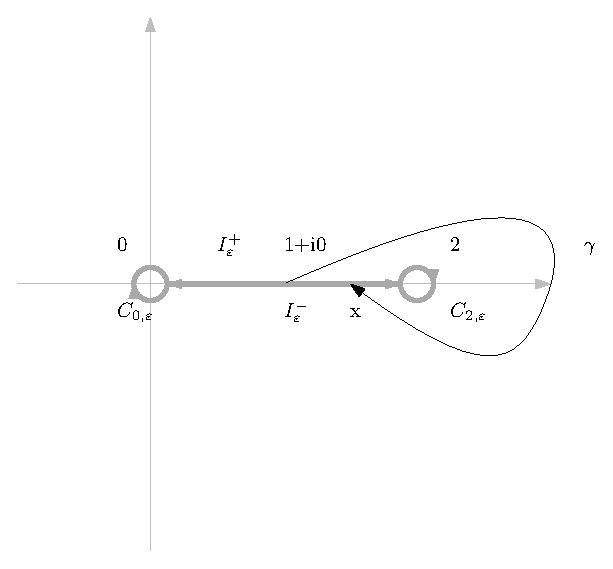
\includegraphics[scale=0.75]{Par18.eps}
		\label{fig:18.1}
\end{figure}
Рассмотрим
\begin{align*}
  & \gamma_\varepsilon = I_\varepsilon^+\cup C_{2, \varepsilon} \cup I_\varepsilon^-\cup C_{0, \varepsilon}
\end{align*}
и
\begin{align*}
  & F(z) = \frac{\sqrt[4]{z^3(2-z)}}{(1+z)^2} = \frac{g(z)}{(1+z)^2}
\end{align*}
и вычислим
\begin{align*}
  & I_\varepsilon = \int_{\gamma_\varepsilon}F(z) dz = 2 i \pi \left( \us{-1}{\res} F(z) + \us{\infty}{\res} F(z) \right)
\end{align*}
Видим, что $-1$~--- полюс $2$ порядка, а $\infty$~--- УОТ.
\begin{align*}
  & \us{-1}{\res} F(z) = \lim_{z \to -1}((z+1)^2F(z))' = \lim_{z \to -1}g'(z) = g'(-1) = \left. \frac{f'(z)}{4g^3(z)}\right|_{z = -1} = \frac{-4(-1)^3+6(-1)^2}{4\left( \sqrt[4]{3}\exp\left( \frac{3i\pi}{4} \right)\right)^3} = \\
  & = \frac{5}{2\sqrt[4]{27}}\exp\left( \frac{-i\pi}{4} \right)
\end{align*}
Рассмотрим $x \in (2; \infty)$; тогда
\begin{align*}
  & g(x) = \sqrt[4]{x^3(2-x)}\exp\left( \frac{-i\pi}{4} \right) = x\sqrt[4]{1-\frac{2}{x}}\exp \left( \frac{-i\pi}{4} \right) = x\exp\left( \frac{-i\pi}{4} \right)\sum_{n=0}^\infty C_{\frac{1}{4}}^n\left( -\frac{2}{x} \right)^n
\end{align*}
Две регулярные функции ($g(x)$ и сумма) совпадают на $(2; \infty)$, а значит, по
теореме единственности
\begin{align*}
  & g(z) = z\exp\left( \frac{-i\pi}{4} \right)\sum_{n=0}^\infty C_{\frac{1}{4}}^n\left( -\frac{2}{z} \right)^n, \ \left| z \right|> 2
\end{align*}
\begin{align*}
  & F(z) = \frac{z}{(z+1)^2}h(z), \ h(z) = \exp\left( \frac{-i\pi}{4} \right)\sum_{n=0}^\infty C_{\frac{1}{4}}^n\left( -\frac{2}{z} \right)^n
\end{align*}
Заметим, что
\begin{align*}
  & \frac{z}{(1+z)^2} = \frac{1}{z(1+\frac{1}{z})^2} = \frac{1}{z} \left( 1-\frac{2}{z} +\frac{3}{z^2} + \dots \right)
\end{align*}
При перемножении двух рядов получим
\begin{align*}
  & \us{\infty}{\res}F(z) = -\exp\left( \frac{-i\pi}{4} \right)
\end{align*}
и интеграл
\begin{align*}
  & I_\varepsilon = 2 i \pi \left( \frac{5}{2\sqrt[4]{27}} - 1 \right)\exp\left( \frac{-i\pi}{4} \right)
\end{align*}
не зависит от $\varepsilon$. Заметим, что
\begin{align*}
  & I_\varepsilon = \int_{I_\varepsilon^+}F(z) + \int_{C_{2, \varepsilon}}F(z) + \int_{I_\varepsilon^-}F(z) + \int_{C_{0, \varepsilon}}F(z)
\end{align*}
Причем
\begin{align*}
  & \int_{I_\varepsilon^+}F(z) = \int_{\varepsilon}^{2-\varepsilon}\frac{\sqrt[4]{x^3(2-x)}}{(x+1)^2}dx
\end{align*}
\begin{align*}
  & \int_{I_\varepsilon^-}F(z) = \int_{2-\varepsilon}^{\varepsilon}\frac{g(x-i0)}{(x+1)^2}dx = -\int_{\varepsilon}^{2-\varepsilon}\frac{\sqrt[4]{x^3(2-x)}\exp\left( \frac{3i\pi}{2} \right)}{(x+1)^2}dx = -\exp\left( \frac{3i\pi}{2}\right) \int_{I_\varepsilon^+}F(z)
\end{align*}
Учтя $z = \varepsilon e^{i \varphi}$,
\begin{align*}
  & \left|  \int_{C_{0, \varepsilon}}F(z) \right| \leq \int_{0}^{2 \pi}\frac{\varepsilon\sqrt[4]{\varepsilon^3(2+\varepsilon)}}{(1-\varepsilon)^2}d\varphi \leq A\varepsilon^{\frac{7}{3}} \us{\varepsilon \to 0}{\to} 0
\end{align*}
Учтя $z = 2 + \varepsilon e^{i \varphi}$,
\begin{align*}
  & \left|  \int_{C_{2, \varepsilon}}F(z) \right| \leq \int_{0}^{2 \pi}\frac{\varepsilon\sqrt[4]{(2+\varepsilon)^3\varepsilon}}{(3-\varepsilon)^2}d\varphi \leq B\varepsilon^{\frac{4}{3}} \us{\varepsilon \to 0}{\to} 0
\end{align*}
Значит,
\begin{align*}
  & 2 i \pi \left( \frac{5}{2\sqrt[4]{27}} - 1 \right)\exp\left( \frac{-i\pi}{4} \right) = I_\varepsilon \us{\varepsilon \to 0}{\to} \int_{I_\varepsilon^+}F(z) + \int_{I_\varepsilon^-}F(z) = \left( 1 -\exp\left( \frac{3i\pi}{2}\right) \right) \int_{I_\varepsilon^+}F(z) \us{\varepsilon \to 0}{\to} \\
  & \us{\varepsilon \to 0}{\to} \left( 1 -\exp\left( \frac{3i\pi}{2}\right) \right) I
\end{align*}
Значит,
\begin{align*}
  & I = \frac{2 i \pi \left( \dst \frac{5}{2\sqrt[4]{27}} - 1 \right)\exp\left( \dst\frac{-i\pi}{4} \right)}{\left( 1 -\exp\left( \dst \frac{3i\pi}{2}\right) \right)}= \pi \sqrt{2}\left( \dst \frac{5}{2\sqrt[4]{27}} - 1 \right)
\end{align*}
\section{$\S 19.$ Целые и мероморфные функции.}
\Def
Функция $f$ называется \textbf{целой}, если она регулярна на $\CC$.
\\
Можем представить такую функцию в виде
\begin{equation}\label{(19.1)}
    \forall z \in \CC \ f(z) = \sum_{n=0}^\infty c_nz^n, \ c_n = \frac{1}{2i\pi}\int_{\gamma_r}\frac{f(\zeta)}{\zeta^{n+1}} d \zeta
\end{equation}
\theorem
Пусть $f:G \mapsto \CC$ целая, $\exists A > 0, \ R > 0, \ m \in \NN_0$ такие,
что $\forall z: \left| z \right| > R \hookrightarrow \left| f(z) \right| \leq
A\left| z \right|^m$. Тогда $f(z)$~--- многочлен степени $\leq m$.
\pr
Воспользуемся оценкой $c_n$.
\begin{align*}
  & \forall r > R \ \left|c_n \right| \leq \frac{1}{2\pi}\int_{\left| \zeta \right| = r} \frac{\left| f(\zeta) \right|}{\left| \zeta \right|^{n+1}}\left| d\zeta \right|\leq \frac{1}{2\pi}\frac{Ar^m}{r^{n+1}}r\cdot 2 \pi = Ar^{m-n}
\end{align*}
Значит, $\forall n > m \ c_n = 0$.
\corollary (теорема Лиувилля)
Если $f$ целая, $\exists R > 0, \ A > 0$: $\left| f(z) \right|< A$ при $\left| z
\right| > R$, то $f \equiv const$.
\theorem (Основная теорема алгебры)
Всякий многочлен $P_n(z) = z^n + C_{n-1}z^{n-1}+\dots+c_0$ имеет в $\CC$ хотя бы
один корень.
\pr
предположим, $\forall z \in \CC \ P_n(z) \neq 0$. Тогда $\varphi(z) = \dst
\frac{1}{P_n(z)}$ целая. Но, как легко видеть,
\begin{align*}
  & \lim_{z \to \infty}P_n(z) = \infty \Rightarrow \lim_{z \to \infty} \varphi(z) = 0 \Rightarrow \exists R > 0: \ \forall z: \ \left| z \right| > R \hookrightarrow \left| \varphi(z) \right| < 1
\end{align*}
Значит, по теореме Лиувилля $\varphi(z) = const$, тогда и $P_n(z) = const$.
Противоречие.
\\
Значит, можем заметить, что для целой функции $f$ единственная особая точка~---
это $\infty$.
\begin{itemize}
    \item $\infty$~--- УОТ, тогда $f = const$.
    \item $\infty$~--- полюс порядка $m$, тогда $f = P_m$.
    \item $\infty$~--- СОТ.
\end{itemize}
\Def
Целая функция, у которой $\infty$ есть СОТ, назвается \textbf{целой
  трансцендентной}.
\theorem (Сохоцкого)
Пусть $f$~--- целая трансцендентная функция, тогда
\begin{align*}
  & \forall A \in \CCC \ \exists z_n \to \infty: \ \lim_{n \to \infty}f(z_n) = A
\end{align*}
\pr
Рассмотрим два случая.
\begin{itemize}
    \item $A = \infty$
    \\
    $f$ неограничена в окрестности $\infty$ (т.~к. иначе она бы имела конечный
    предел), т.~е.
    \begin{align*}
      & \forall n \in \NN \ \exists z_n \in \CC: \left| f(z_n) \right|> n, \ \left| z_n \right| > n
    \end{align*}
    Итак, $\left\{ z_n \right\}$ и есть та самая последовательность.
    \item $A \in \CC$
    \\
    Пусть, от противного,
    \begin{align*}
      & \exists \delta_0 > 0, \ \varepsilon_0 > 0: \ \forall z: \ \left| z \right| \geq \delta_0 \ \left| f(z) - A \right| \geq \varepsilon_0
    \end{align*}
    Пусть $\varphi(z) = \dst \frac{1}{f(z) - A}$, $z \in B_{\delta_0}(\infty)$.
    На этом множестве
    \begin{align*}
      & \left| \varphi(z) \right| \leq \frac{1}{\varepsilon_0}
    \end{align*}
    Значит, эта функция на этом множестве регулярна и ограничена, а значит, для
    нее $\infty$~--- УОТ, т.~е.
    \begin{align*}
      & \exists \lim_{z \to \infty}\varphi(z) = B
    \end{align*}
    Значит, $\infty$~--- полюс либо УОТ для $f(z)$, противоречие.
\end{itemize}
\theorem (общая теорема Сохоцкого)
Пусть $f: \os{\circ}{B}_r(a) \mapsto \CC$ регулярна, $a$~--- СОТ $f$. Тогда
\begin{align*}
  & \forall A \in \CCC \ \exists z_n \to a, \ \lim_{n \to \infty} f(z_n) = A
\end{align*}
\Exse
доказать общую теорему Сохоцкого.
\theorem (Пикара)
Пусть $f$~--- целая трансцедентная функция, тогда $\forall a \in \CC$, за
исключением, быть может, одного, $\exists R > 0$: в $\os{\circ}{B}_R(\infty)$
существует бесконечное число решений уравнения $f(z) = A$, т.~е.
\begin{align*}
  & \exists z_n \to \infty: \ \forall n \in \NN \ f(z_n) = A
\end{align*}
\Example
$e^z = A$ имеет счетное число решений в любой окрестности бесконечности при $A
\neq 0$, но ни одного решения при $A = 0$.
\Exse
Пусть $f$~--- целая функция и
\begin{align*}
  & \exists A > 0, R > 0, \ m \in \NN_0: \ \forall z: \ \left| z \right| > R \ \left| f(z) \right| \geq A \left| z \right|^m
\end{align*}
Доказать, что $f$~--- многочлен степени $\leq m$.
\Def
Функция $f$ называется мероморфной, если $\forall R > 0$ в круге $B_R(0)$ она
регулярна за исключением, быть может, конечного числа полюсов.
\Example
\begin{align*}
  & f(z) = \frac{P_n(z)}{Q_m(z)}
\end{align*}
Конечное число полюсов на всей $\CC$.
\Example
\begin{align*}
  & f(z) = \ctg z
\end{align*}
Счетное число полюсов на $\CC$.
\Example
\begin{align*}
  & f(z) = \frac{z}{e^z-1}
\end{align*}
Счетное число полюсов на $\CC$.
    \begin{flushright}
    \textit{Лекция 15 (от 26.10)}
\end{flushright}
$f$ мероморфна~--- тогда существует $\left\{ z_k \right\}_{n=1}^{\infty}$~---
полюсы $m_k$ порядков.
\\
Тогда $\exists \os{\circ}{B}_{\delta_k}(z_k)$, где ряд Лорана
\begin{equation}\label{(19.2)}
    f(z) = \frac{c^k_{-m_k}}{(z-z_k)^{m_k}} + \dots + \frac{c^k_{-1}}{z-z_k} + c_0^k= c_1^k(z-z_k) + \dots
\end{equation}
а его главная часть
\begin{equation}\label{(19.3)}
    q_k(z) = \frac{c^k_{-m_k}}{(z-z_k)^{m_k}} + \dots + \frac{c^k_{-1}}{z-z_k}
\end{equation}
\theorem
Пусть $f$ мероморфна, $\infty$~--- УОТ или полюс этой функции. Тогда $f$
рациональна.
\pr
$\left\{ z_k \right\}$~--- полюсы $m_k$ порядка. В силу изолированности $\infty$
набор полюсов конечен; пусть $k \in \left\{ 1, \dots, l \right\}$.
\\
$\infty$~--- УОТ или полюс; главная часть ряда Лорана в окрестности $\infty$
будет иметь вид
\begin{align*}
  & q_0 = c_1z+\dots +c_nz^n
\end{align*}
Из \eqref{(19.3)} получим $q_k(z)$ для любого $k$.
\\
Тогда
\begin{equation}\label{(19.4)}
    r(z) = f(z) - \sum_{k=0}^lq_k(z)
\end{equation}
Заметим, что $\forall k$ $r(z)$ имеет в $z_k$ устранимую особую точку. Эта
функция, доопределенная по непрерывности, будет регулярной в $\CC$ и
ограниченной на бесконечности, а значит, по теореме Лиувилля $r(z) \equiv a_0$.
Тогда из \eqref{(19.4)} получим
\begin{align*}
  & f(z) = a_0 + \sum_{k=0}^lq_k(z)
\end{align*}
а значит, $f$ рациональна.
\Def
Совокупность замкнутых простых кусочно гладких кривых $\left\{ \Gamma_n
\right\}_{n=1}^\infty$ называется \textbf{правильной}, если
\begin{itemize}
    \item $\forall n \in \NN$ область $D_n$, ограниченная $\Gamma_n$, содержится
    в области $D_{n+1}$, ограниченной $\Gamma_{n+1}$, причем $0 \in D_1$;
    \item $d_n = \min \left\{ \left| z \right| : z \in \Gamma_n \right\}
    \Rightarrow \dst \lim_{n \to \infty}d_n = \infty$;
    \item $\exists A > 0: \ \forall n \in \NN \ l_n \leq Ad_n$, где $l_n  =
    l(\Gamma_n)$.
\end{itemize}
\example
Вложенные окружности, вложенные квадраты с центром в точке $0$.
\theorem (Коши)
Пусть $f$ мероморфна и существует правильная совокупность $\left\{ \Gamma_n
\right\}_{n=1}^\infty$, такая, что:
\begin{itemize}
    \item $\varepsilon_n = \max\left\{ \left| f(z) \right|: z \in \Gamma_n
    \right\}: \ \dst \lim_{n \to \infty}\varepsilon_n = 0$
    \item $\left\{ z_n \right\}$~--- полюса, пронумерованные так, что $\forall n
    \in \NN$ в $D_n$ содержится ровно $n$ первых полюсов, а на $\Gamma_n$ полюсов
    нет.
\end{itemize}
Тогда $f(z)$ может быть представлена в виде ряда элементарных дробей:
\begin{equation}\label{(19.5)}
    f(z) = \sum_{k=1}^\infty q_k(z)
\end{equation}
причем $q_k$ определяется из \eqref{(19.3)}, а ряд \eqref{(19.5)} сходится
равномерно $\forall R > 0$ в $B_R(0)$ (за исключением полюсов).
\pr
$\forall n \in \NN$ определим
\begin{equation}\label{(19.6)}
    S_n(z) = \sum_{k=1}^n q_k(z)
\end{equation}
\begin{equation}\label{(19.7)}
    r_n(z) = f(z) - S_n(z)
\end{equation}
Фиксируем $n$, доопределяем $r_n$ в $D_n$ по непрерывности. Тогда эта функция
будет регулярной в этой области и непрерывной на ее границе $\Gamma_n$, а
значит, и на замыкании. По интегральной формуле Коши $\forall z \in D_n$
\begin{align*}
  & r_n(z) = \frac{1}{2 i \pi}\int_{\Gamma_n}\frac{r_n(\zeta)}{\zeta - z}d\zeta = \frac{1}{2 i \pi}\int_{\Gamma_n}\frac{f(\zeta)}{\zeta - z}d\zeta - \frac{1}{2 i \pi}\int_{\Gamma_n}\frac{S_n(\zeta)}{\zeta - z}d\zeta
\end{align*}
У функции $F_n(\zeta) = \dst \frac{S_n(\zeta)}{\zeta - z}$ внутри $D_n$ все
соответствующие $z_k$~--- особые точки, а вне $D_n$~--- $\infty$.
\begin{align*}
  & -\frac{1}{2 i \pi}\int_{\Gamma_n}F_n(\zeta) d\zeta = \us{\infty}{\res}F_n(\zeta)
\end{align*}
\begin{align*}
  & F_n(\zeta) = \sum_{k=1}^n\sum_{l=1}^{m_k}\frac{c_{-l}^k}{(\zeta - z)(\zeta - z_k)^{l}}
\end{align*}
Т.~к. $l+1 > 1$, то вычет равен нулю. Значит,
\begin{equation}\label{(19.8)}
    r_n(z) = \frac{1}{2 i \pi}\int_{\Gamma_n}\frac{f(\zeta)}{\zeta - z}d\zeta
\end{equation}
Фиксируем $R>0$. Тогда, в силу $d_n \to \infty$, $\exists N: \ \forall n \geq N
\ d_n > 2R$, и тогда
\begin{align*}
  & \left| r_n \right| \leq \frac{1}{2\pi}\us{\zeta \in \Gamma_n}{\max}\left| \frac{f(\zeta)}{\zeta - z} \right| l_n = \frac{\varepsilon_n l_n}{2\pi (d_n - R)} \leq \frac{\varepsilon_n}{\pi}A = \frac{A}{\pi}\varepsilon_n
\end{align*}
Значит, в $B_R(0)$ $r_n \rightrightarrows 0$. Соответственно, $S_n
\rightrightarrows f(z)$ в $B_R(0) \setminus \left( \dst
    \bigcup_{k=1}^{\infty}\left\{ z_k \right\} \right)$.
\Note
Пусть в тереме $7$ условие $\varepsilon_n \to 0$ заменено на $\exists B > 0, \ m
\in \NN: \ \varepsilon_n \leq Bd_n^m$. Тогда все условия теоремы $7$ выполняются
для функции $\dst \frac{f(z)}{z^{m+1}}$.
\pr (заметка)
В случае, если $0$ не является особой точкой, нужно добавить $\Gamma_0$~--- круг
малого радиуса с центром в нуле, лежащий в области $D_1$. Видим, что функция
$f(z)$, как и функция из замечания, разложима в этом случае в ряд элементарных
дробей.
\Example
Разложить в ряд элементарных дробей $w = \ctg z$.
\\
Знаем, что $z = \pi k, \ k \in \ZZ$~--- особые точки этой мероморфной функции.
Построим соответствующую правильную систему контуров.
\\
Положим $\tilde{z}_1 = 0$, $\tilde{z}_2 = \pi$, $\tilde{z}_3 = -\pi$,
$\tilde{z}_4 = 2 \pi$ и т.~д. Построим систему контуров:
% \begin{figure}[h!]
% 		\centering
% 		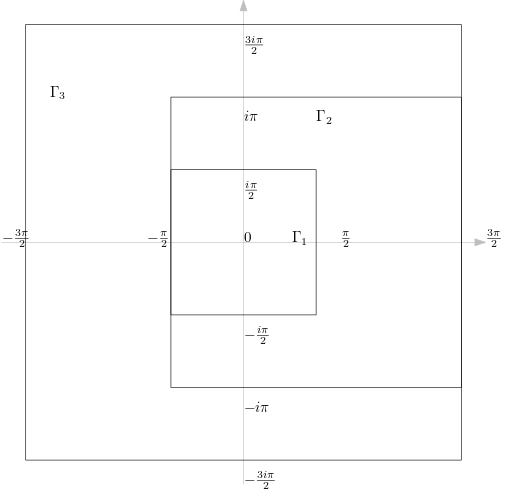
\includegraphics[scale=0.5]{Par20.png}
% 		\label{fig:19.1}
% \end{figure}
\begin{figure}[h!]
		\centering
		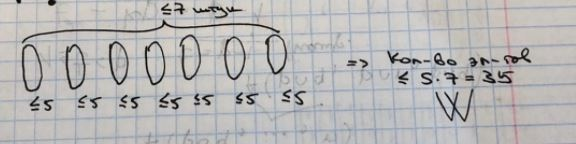
\includegraphics[scale=1]{20}
		\label{fig:19.2}
\end{figure}
Заметим, что $\Gamma_n$~--- квадраты, $l_n = 4\pi n$, $d_n \geq (n-1)\dst
\frac{\pi}{2}$, $\dst \frac{l_n}{d_n}\leq 16$. Значит, система контуров
правильная.
\\
Рассмотрим условия теоремы $7$. На вертикальных границах $\Gamma_n$ $z = \dst
\frac{\pi}{2} + \pi m + iy$. Тогда
\begin{align*}
  & \left| f(z) \right| = \frac{\left| \cos\left( \frac{\pi}{2}+\pi m + iy \right) \right|}{\left| \sin\left( \frac{\pi}{2}+\pi m + iy \right) \right|} = \frac{\left| \sin(iy) \right|}{\left| \cos(iy) \right|} = \frac{\left| e^{-y} - e^y \right|}{\left| e^{-y}+e^y \right|} \leq 1
\end{align*}
Видим, что функция ограничена на них. На горизонтальных границах $\Gamma_n$ $z =
x \pm i \dst \frac{\pi n}{2} = x+iy_n$. Тогда
\begin{align*}
  & \left| f(z) \right| = \frac{\left| e^{-y_n+ix}+e^{y_n-ix} \right|}{\left| e^{-y_n+ix}+e^{y_n-ix} \right|} \leq \frac{\left| e^{-y_n}+e^{y_n} \right|}{\left| e^{-y_n}+e^{y_n} \right|} \leq \frac{ 1+e^{-2\abs{y_n}}}{ 1-e^{-2\abs{y_n}}} \leq 2
\end{align*}
Видим, что функция ограничена на них.
\\
По замечанию $1$ $\dst \frac{\ctg z}{z}$ удовлетворяет условиям теоремы $7$, а
значит, $z = 0$~--- полюс второго порядка, $z_k = \pi k$~--- полюса первого
порядка, и тогда
\begin{align*}
  & \frac{\ctg z}{z} = \frac{\cos z}{z \sin z} = \frac{1 - \dst \frac{z^2}{2!} +\dots}{z^2 - \dst \frac{z^4}{3!}+\dots} = \frac{1}{z^2} +c_0 + c_1z + \dots
\end{align*}
\begin{align*}
  & q_0(z) = \frac{1}{z^2}
\end{align*}
\begin{align*}
  & z_k = \pi k, \ k \neq 0
\end{align*}
Значит,
\begin{align*}
  &  q_k = \frac{\us{\pi k}{\res}\dst \frac{\ctg z}{z}}{z - \pi k} = \frac{1}{\pi k (z - \pi k)}
\end{align*}
\begin{align*}
  & \frac{\ctg z}{z} = \frac{1}{z^2} +\sum_{^{k=-\infty}_{k \neq 0}}^{+\infty}\frac{1}{\pi k (z-\pi k)}
\end{align*}
\begin{align*}
  & \ctg z = \frac{1}{z} +\sum_{^{k=-\infty}_{k \neq 0}}^{+\infty}\frac{z+\pi k -\pi k}{\pi k (z-\pi k)} = \frac{1}{z} +\sum_{^{k=-\infty}_{k \neq 0}}^{+\infty}\left( \frac{1}{\pi k} + \frac{1}{z-\pi k}\right) = \frac{1}{z} +\sum_{k=1}^{\infty}\left( \frac{1}{\pi k} + \frac{1}{z-\pi k} + \frac{1}{-\pi k} + \right. \\
  &\left. \frac{1}{z+\pi k}\right) = \frac{1}{z} +\sum_{k=1}^{\infty}\left( \frac{1}{z-\pi k} + \frac{1}{z+\pi k}\right)
\end{align*}
\section{$\S 20.$ Принцип аргумента. Теорема Руше.}
\theorem
Пусть $f: G \mapsto \CC$
Пусть $G$~--- односвязная облась в $\CC$, $\ogamma$~--- простая замкнута
положительно ориентированная кривая в этой области. Пусть $f: G \mapsto \CC$
регулярна в $G$ за исключением, быть может, полюсов $a_1, \dots, a_k, \dots$,
лежащих внутри $\ogamma$. Пусть на $\ogamma$ нет особых точек $f$. Тогда
справедливо:
\begin{equation}\label{(20.1)}
    \frac{1}{2 i \pi}\int_{\ogamma} \frac{f'(z)}{f(z)}dz = N - P
\end{equation}
где $N$~--- число нулей, $P$~--- полюсов с учетом их порядка (каждый ноль или
полюс считаем такое число раз, каков его порядок)).
\pr
Пусть $b_1, \dots, b_n$~--- нули $f$ внутри $\ogamma$. В силу компактности
ограниченной $\ogamma$ области вместе с кривой и того. что $f(z) \not \equiv 0$,
их конечное число.
\\
Рассмотрим любой нуль $b = b_k$ порядка $m$. Тогда
\begin{align*}
  & f(z) = (z-b)^mh(z), \ z \in B_\varepsilon(b), \ \forall z \in B_\varepsilon(b) \ h(z) \neq 0
\end{align*}
Тогда
\begin{align*}
  & \frac{f'(z)}{f(z)} = \frac{m(z-b)^{m-1}h(z)+(z-b)^mh'(z)}{(z-b)^mh(z)} = \frac{m}{z-b} + \frac{h'(z)}{h(z)}
\end{align*}
и, значит,
\begin{align*}
  & \us{b}{\res}\frac{f'(z)}{f(z)} = m
\end{align*}
Пусть $a_1, \dots, a_p$~--- полюса, их, аналогично, тоже конечное число.
\\
Рассмотрим произвольный полюс $a = a_k$ порядка $l$. Тогда
\begin{align*}
& f(z) = \frac{p(z)}{(z-a)^l}, z \in \os{\circ}{B}_\delta(a), \ \forall z \in \os{\circ}{B}_\delta
(a) \ p(z)\neq 0
\end{align*}
Тогда
\begin{align*}
  & \frac{f'(z)}{f(z)} = \frac{-l}{z-a} + \frac{p'(z)}{p(z)}
\end{align*}
\begin{align*}
  & \us{a}{\res}\frac{f'(z)}{f(z)} = -l
\end{align*}
Отсюда по теореме Коши имеем \eqref{(20.1)}
\corollary (принцип аргумента)
В условии теорем $20.1$
\begin{equation}\label{(20.2)}
  \frac{1}{2\pi} \Delta_{\ogamma}\argt f(z) = N - P
\end{equation}
\pr
Пусть $\ogamma: z = z(t)$, $z(0) = z(1)$, $\ogamma$~--- гладкая замкнутая кривая.
\\
Пусть $\os{\circ}{\Gamma} = f(\ogamma)$, $0 \not \in \os{\circ}{\Gamma}$, $w =
f(z(t))$, $t \in [0;1]$.
\\
Тогда
\begin{align*}
  & \Real \int_{\os{\circ}{\Gamma}}\frac{dw}{w} = \Real \int_{\os{\circ}{\gamma}}\frac{f'(z)}{f(z)}dz = \ln\left| w \right| \Big|_{f(z(1))}^{f(z(0))} = 0
\end{align*}
\begin{align*}
  & \Img \int_{\os{\circ}{\Gamma}}\frac{dw}{w} = \Img \int_{\os{\circ}{\gamma}}\frac{f'(z)}{f(z)}dz = \Delta_{\ogamma}\argt f(z)
\end{align*}
\begin{align*}
  & \int_{\os{\circ}{\gamma}}\frac{f'(z)}{f(z)}dz = i\Delta_{\ogamma}\argt f(z)
\end{align*}
Тогда из \eqref{(20.1)} очевидно следует \eqref{(20.2)}.
    \begin{flushright}
    \textit{Лекция 16 (от 27.10)}
\end{flushright}
\theorem (Руше)
Пусть $G$~--- односвязная область, $\ogamma$~--- замкнутая положительно
ориентированная кусочно гладкая кривая в этой области. Пусть $f,g: G \mapsto
\CC$ регулярны, и
\begin{equation}\label{(20.3)}
    \forall z \in \ogamma \ \left| f(z) \right| > \left| g(z) \right|
\end{equation}
Тогда $f(z)$ и $h(z) = f(z)+g(z)$ имеют внутри $\ogamma$ одинаковое число нулей
с учетом их порядка.
\pr
\begin{align*}
  & \forall z \in \ogamma \ \left| f(z) \right| > \left| g(z) \right| \Rightarrow \forall z \in \ogamma \ f(z) \neq 0
\end{align*}
\begin{align*}
  & \forall z \in \ogamma \ \left| h(z) \right|\geq \left| f(z) \right| - \left| g(z) \right| > 0 \Rightarrow \forall z \in \ogamma h(z) \neq 0
\end{align*}
\begin{align*}
  & \Delta_{\ogamma}\argt h(z) = \Delta_{\ogamma} \argt \left( f(z)\left( 1+\frac{g(z)}{f(z)} \right) \right) = \Delta_{\ogamma}\argt f(z) +\Delta_{\ogamma}\argt \left( 1+\frac{g(z)}{f(z)} \right)
\end{align*}
\begin{align*}
  & \ogamma: w = 1 + \frac{g(z)}{f(z)} \Rightarrow \left| w-1 \right| = \left| \frac{g(z)}{f(z)} \right| < 1
\end{align*}
Пусть $\Gamma = w(\ogamma) \subseteq B_1(1)$; $0 \not \in B_1(1)$ и эта область
односвязна, значит, по теореме $3$ $\S 14$
\begin{align*}
  & \Delta_{\ogamma}\argt \left( 1+\frac{g(z)}{f(z)} \right) = 0
\end{align*}
и тогда
\begin{align*}
  & N_h = \frac{1}{2\pi}\Delta_{\ogamma}\argt h(z) = \frac{1}{2\pi}\Delta_{\ogamma}\argt f(z) = N_f
\end{align*}
\theorem (Гаусса)
Многочлен
\begin{align*}
  & P_n(z) = c_0+zc_1+z^2c_2+\dots+z^nc_n
\end{align*}
имеет в $\CC$ ровно $n$ корней с учетом их порядка.
\pr
Рассмотрим $f(z) = c_nz^n$, $g(z) = P_n(z) - f(z)$. Как известно,
\begin{align*}
  & \left| \frac{g(z)}{f(z)} \right| \us{z \to \infty}{\to} 0 \Rightarrow \exists R_0 > 0: \ \forall R \geq R_0 \ \forall z \in \gamma_R \ \left| f(z) \right| > \left| g(z) \right|
\end{align*}
Значит, по теореме Руше функция $P_n(z)$ имеет столько же нулей, сколько и $f(z)
= c_nz^n$, на $B_R(0)$, с учетом порядка, т.~е. ровно $n$ штук.
\Example
Функция Жуковского
\begin{align*}
  & w = \frac{1}{2}\left( z+\frac{1}{z} \right)
\end{align*}
У функции $\pm i$~--- нули, $0$~--- полюс первого порядка.
\\
Рассматривая $R>1$, получим
\begin{align*}
  & \Delta_{\gamma_R}\argt w(z) = 2 \pi (N-P) = 2\pi
\end{align*}
\begin{align*}
  & \Delta_{\gamma_{\frac{1}{R}}}\argt w(z) = 2 \pi (N-P) = -2\pi
\end{align*}
\section{$\S 21.$ Геометрические принципы.}
\lemma (об открытости)
Пусть $f$ регулярна в $G$, $z_0 \in G$, $w_0 = f(z_0)$.
\\
Пусть при $n \geq 2$
\begin{equation}\label{(21.1)}
    f'(z_0) = \dots = f^{(n-1)}(z_0) = 0, \ f^{(n)}(z_0) \neq 0
\end{equation}
Тогда $\exists B_\delta(z_0)$ и $B_\varepsilon(w_0)$, такие, что $\forall w_1
\in B_{\varepsilon}(w_0)$ уравнение $f(z) = w_1$ имеет в круге $B_\delta(z_0)$
ровно $n$ решений.
\pr
Заметим, что $f(z) \neq const$, $f'(z) \neq const$. Тогда по теореме
единственности нули функции $f(z)-w_0$ и $f'(z)$ изолированы, поэтому
\begin{align*}
  & \exists \delta > 0: \ \forall z \in \ol{\os{\circ}B_\delta(z_0)}\setminus\{z_0\} \ f(z)-w_0 \neq 0, \ f'(z) \neq 0
\end{align*}
Пусть $\gamma = \left\{ z: \left| z-z_0 \right| = \delta \right\}$ положительно
ориентирована, и $\forall z \in \gamma \ f(z)\neq w_0$. Положим $0 < \varepsilon
= \inf \left\{ w_0 - f(z) \mid z \in \gamma \right\}$, $\Gamma = f(\gamma)$.
заметим, что $\Gamma$ замкнута и $w_0 \not \in \Gamma$.
\\
Тогда
\begin{align*}
& \forall w_1 \in \os{\circ}{B}_\varepsilon(w_0), \ \forall z \in \gamma \ \left| w_1-w_0 \right| < \varepsilon \leq \left| w_0 - f(z) \right|
\end{align*}
Пусть $F(z) = w_0 - f(z)$, $G(z) = w_1-w_0$. Тогда $H(z) = F(z)+G(z) =
w_1-f(z)$; значит, по теореме Руше (в силу $\left| F(z) \right|> \left| G(z)
\right|$) функции $w_0 - f(z)$ и $w_1-f(z)$ имеют одинаковое число нулей внутри
$\gamma$. 
\\
Заметим, что $f(z) = w_0$ имеет единственный нуль~--- $z_0$~--- порядка $n$.
Значит, с учетом порядка $f(z) = w_1$ имеет $n$ решений.
\\
Но 
\begin{align*}
& \forall z \in B_\delta(z_0) \ f'(z) = (f(z)-w_1)' \neq 0
\end{align*}
Значит, все нули будут иметь первый порядок, соответственно, их ровно $n$ штук.
\corollary
Пусть $f$ регулярна в $G \subseteq \CC$. Тогда $\forall z_0 \in G$ условие
$f'(z_0) \neq 0$ необходимо и достаточно для однолистности $f$ <<в малом>>~--- в
некоторой достаточно малой окрестности $z_0$, но не во всей $G$.
\Example
$w=e^z$ удовлетворяет условиям следствия, но не однолистна во всей комплексной
плоскости.
\theorem (принцип сохранения области)
Пусть $f$ регулярна в области $G$, причем $f(z) \neq const$. Тогда $f(G)$~---
также область.
\pr
Докажем открытость.
\begin{align*}
& \forall z_0 \in G \ w_0 = f(z_0) \in G^* = f(G)
\end{align*}
Поскольку $G$~--- область, 
\begin{align*}
& \exists \delta_1: \ B_{\delta_1}(z_0) \subseteq G
\end{align*}
и по лемме $21.1$
\begin{align*}
& \exists \delta \in (0; \delta_1], \ \exists \varepsilon > 0: \ \forall w_1 \in B_\varepsilon (w_0) \ \exists z_1 \in B_\delta(z_0): \ f(z_1) = w_1; \ f(B_\delta(z_0)) \supseteq B_\varepsilon(w_0)
\end{align*}
Значит, $B_\varepsilon(w_0)\subseteq G^*$, т.~е. $w_0$~--- внутренняя точка $G^*$.
\\
Докажем связность.
\begin{align*}
  & \forall w_1, w_2 \in G^* \ \exists z_1,z_2 \in G: \ \exists \gamma_{z_1z_2} \subseteq G, \ \Gamma_{w_1w_2} = f(\gamma_{z_1z_2}) \subseteq G^*
\end{align*}
\theorem (принцип максимума модуля регулярной функции)
Пусть $f: G \mapsto \CC$ регулярна в ограниченной области $G$, непрерывна на ее
замыкании и непостоянна. Тогда
\begin{align*}
  & \max_{z \in \ol{G}} \left| f(z) \right| = \max_{z \in \partial G} \left| f(z) \right|
\end{align*}
\pr
Путь, от противного,
\begin{align*}
  & \exists z_0 \in G: \ \left| f(z_0) \right| = \max_{z \in \ol{G}}\left| f(z) \right|
\end{align*}
Пусть $w_0 = f(z_0)$. По теореме $21.1$
\begin{align*}
  & \exists \varepsilon > 0, \ B_\varepsilon(w_0) \subseteq f(G) = G^*
\end{align*}
\begin{align*}
  & w_1 \in B_\varepsilon(w_0): \left| w_1 \right| > \left| w_0 \right|; \ w_1 = w_0\left( 1+\frac{\varepsilon}{2\left| w_0 \right|} \right)
\end{align*}
\begin{align*}
  & \exists z_1 \in G: \ f(z_1) = w_1; \ \left| f(z_1) \right| > \left| f(z_0) \right|
\end{align*}
Противоречие.
\corollary (принцип минимума модуля регулярной функции)
Пусть $f: G \mapsto \CC$ регулярна в ограниченной области $G$, непрерывна на ее
замыкании и непостоянна; $\forall z \in G \ f(z) \neq 0$. Тогда
\begin{align*}
  & \min_{z \in \ol{G}} \left| f(z) \right| = \min_{z \in \partial G} \left| f(z) \right|
\end{align*}
\Note
Для случая неограниченной $G$ вместо $\min$ и $\max$ используется $\inf$ и
$\sup$.
\lemma (Шварца)
Пусть $f: B_1(0) \mapsto \CC$ регулярна, $\forall z \in B_1(0) \ \left| f(z)
\right| \leq 1$, $f(0) = 0$. Тогда выполняется
\begin{equation}\label{(21.2)}
    \forall z \in B_1(0) \ \left| f(z) \right| \leq z
\end{equation}
Если в \eqref{(21.2)} достигается равенство при $z_0 \neq 0$, то
\begin{align*}
  & \exists \alpha \in \RR: \ \forall z \in \ol{B_1(0)} \ f(z) = e^{i\alpha}z
\end{align*}
\pr
$f(0) = 0$, а значит, существует регулярная в $B_1(0)$ функция $g(z)$: $f(z) =
zg(z)$. Функция $g(z) = \dst \frac{f(z)}{z}$, но при этом регулярна также и в
нуле.
\\
Рассмотрим произвольное $r \in (0;1)$ и $z: \ \left| z \right|<r$. По теореме
$2$
\begin{align*}
  & \left| g(z) \right| \leq \max \left\{ \left| \frac{f(\zeta)}{\zeta} \right| : \left| \zeta \right| =r \right\} \leq \frac{1}{r}
\end{align*}
Пусть $z_0 \in B_1(0)$; $\forall r \in (\left| z_0 \right|, 1)$ $\left| g(z_0)
\right| \leq \dst \frac{1}{r}$, а значит, $\left| g(z_0) \right|\leq 1$, и
$\forall z \in B_1(0) \ \left| f(z) \right|\leq \left| z \right|$.
\\
Пусть равенство в \eqref{(20.2)} достигается в некоторой точке $z_1$ (т.~е.
$\left| g(z) \right| = 1$). Поскольку точка лежит внутри области, то либо
возникает противоречие с принципом максимума, либо $g(z) = const = e^{i
  \alpha}$.
\theorem (принцип максимума и минимума гармонической функции)
Пусть $u: G \mapsto \CC$ гармоническая на $G \subseteq \RR^2$ и непостоянная,
непрерывная на $\ol{G}$. Тогда $\sup$ и $\inf$ функции $u$ на $G$ и $\ol{G}$
совпадают.
\pr
Допустим, $\exists z_0 = (x_0, y_0)\in G$, на которой $u$ достигает максимума.
Тогда $\exists \varepsilon > 0: \ B_\varepsilon(z_0)\subseteq G$; по теореме $2$
$\S 4$ сущствует регулярная $f$ в $B_\varepsilon(z_0)$ такая, что $\Real f(z) =
u(z)$.
\\
$w_0 = f(z_0)$; по теореме $21.1$ $f(B_\varepsilon(z_0))$~--- область, т.~е.
$\exists r > 0$: $B_r(w_0) \subseteq f(B_{\varepsilon}(z_0))$. Пусть $w_1 \in
B_r(w_0)$, $\Real w_1 > \Real w_0$.
\\
Значит,
\begin{align*}
  \exists z_1 \in B_\varepsilon(z_0): \ w_1 = f(z_1), \ \Real f(z_1) > \Real f(z_0) \Rightarrow u(z_1)>u(z_0)
\end{align*}
Противоречие.
\\
В силу $\inf u(z) = - \sup(-u(z))$, гармоничности $-u(z)$ и выполнимости
принципа максимума выполняется и принцип миминума.
\theorem (о среднем для гармонической функции)
Пусть $u: B_R(z) \mapsto \RR$ гармоническая и непрерывная на замыкании
этого круга, непостоянная. Тогда
\begin{equation}\label{(21.3)}
    u(a) = \frac{1}{2\pi}\int_0^{2\pi}u(a+Re^{i\varphi})d\varphi
\end{equation}
\pr
По теореме $2$ $\S 4$ существует $f: B_R(a) \mapsto \CC$~--- регулярная, причем
$\forall z \in B_R(a) \ \Real f(z) = u(z)$, $0<\rho < R$, $\gamma_\rho =
\left\{ z: \left| z-a \right| = \rho\right\}$.
\begin{align*}
  & f(a) = \frac{1}{2 i \pi}\int_{\gamma_\rho}\frac{f(\zeta)}{\zeta - a}d\zeta = \frac{1}{2i\pi}\int_0^{2\pi}\frac{f(a+\rho e^{i\varphi})}{\rho e^{i\varphi}} i \rho e^{i\varphi} d \varphi = \frac{1}{2\pi}\int_0^{2\pi}f(a+\rho e^{i\varphi})d \varphi
\end{align*}
\begin{align*}
  & \Real f(a) = u(a) = \frac{1}{2\pi}\int_0^{2\pi}\Real f(a+\rho e^{i\varphi})d \varphi = \frac{1}{2\pi}\int_0^{2\pi}u (a+\rho e^{i\varphi})d \varphi
\end{align*}
Устремляя $\rho \to R$, получаем \eqref{(21.3)}.

    \begin{flushright}
    \textit{Лекция 17 (от 02.11)}
\end{flushright}
\section{$\S 22.$ Конформные отображения в $\overline{\CC}$.}
\begin{center}
    \textbf{Геометрический смысл аргумента и модуля производной}
\end{center}
Рассмотрим $f: B_r(z_0) \mapsto \CC$, $f'(z_0) \neq 0$.
\\
Пусть $w = f(z)$, $w_0 = f(z_0)$, $w-w_0 = f'(z_0)(z-z_0) + o(z-z_0)$.
\\
Покоординатно:
\begin{align*}
  & f'(z_0) = u_x+iv_x, \ f=u+iv
\end{align*}
\begin{align*}
  & \left( \begin{matrix}
          \Delta u \\
          \Delta v
      \end{matrix} \right) = \left( \begin{matrix}
          u_x & -v_x \\
          v_x & u_x
      \end{matrix} \right)  \left( \begin{matrix}
          \Delta x \\
          \Delta y
      \end{matrix} \right) = K \left( \begin{matrix}
          \frac{u_x}{K} & \frac{-v_x}{K} \\
          \frac{v_x}{K} & \frac{u_x}{K}
      \end{matrix} \right) \left( \begin{matrix}
          \Delta x \\
          \Delta y
      \end{matrix} \right)
\end{align*}
\begin{align*}
  & K = \sqrt{u^2_x+v^2_x} = \left| f'(z_0) \right|
\end{align*}
Видим, что это ортогональное преобразование.
\\
\textbf{Свойство сохранения окружности в малом:}
\\
Рассмотрим $\gamma_r = \left\{ z: \left| z-z_0 \right| = r, \ 0 < r <
    r_0\right\}$. Пусть в области, ограниченной кривой, производная ненулевая.
\begin{align*}
  & \left| \Delta w \right| \approx \left| f'(z_0) \right|\cdot \left| \Delta z \right| \approx K r
\end{align*}
(получаем <<примерно окружность>>).
\\
\textbf{Свойство сохранения углов:}
\\
Рассмотрим теперь $\gamma_1, \gamma_2: \ z = z_k(t), \ t \in \left[ t_0 -\delta;
    t_0+\delta\right], \ z_k(t_0) = z_0$. Пусть при таких $t$ $z'_k\neq 0$, угол
между кривыми $\alpha$. Пусть $\gamma_1^* = f(\gamma_1)$, $\gamma_2^* =
f(\gamma_2)$. Тогда угол между $\gamma_1^*$ и $\gamma_2^*$ также равен $\alpha$.
\\
Действительно,
\begin{align*}
  & w'_k(t_0) = f'(z_0)z'_k(t_0)
\end{align*}
\begin{align*}
  & \Arg w'_k(t_0) = \argm f'(z_0) + \Arg z'_k(t_0)
\end{align*}
(изменение на одинаковый угол).
\begin{center}
    \textbf{Конформные отображения в $\CC$}
\end{center}
\Def
Функция $f: G \mapsto \CC$ называется \textbf{конформной в точке $z_0$}, если
$f= u+iv$, $u$ и $v$ дифференцируемы в $z_0$ и линейное отображение вида
\begin{equation}\label{(22.1)}
    \begin{cases}
        du = u_x(x_0,y_0)\Delta x + u_y(x_0,y_0) \Delta y \\
        dv = v_x(x_0,y_0)\Delta x + v_y(x_0,y_0) \Delta y
    \end{cases}
\end{equation}
является суперпозицией линейного растяжения и поворота относительно нуля.
\theorem
Функция $f$ конформна в $Z_0 \in \CC$ тогда и только тогда, когда она в этой
точке дифференцируема, а производная отлична от нуля.
\pr
~
\begin{itemize}
    \item $\Leftarrow$
    \\
    Следует из геометрического смысла и определения.
    \item $\Rightarrow$
    \\
    Пусть $f$ конформна в $z_0$. Тогда $\exists K > 0$, $\exists \theta \in
    [0;2\pi)$ такие, что из \eqref{(22.1)} получаем
    \begin{equation}\label{(22.2)}
        \left( \begin{matrix}
                \Delta u \\
                \Delta v
            \end{matrix} \right) = K \left( \begin{matrix}
                \cos \theta & \sin \theta \\
                -\sin \theta & \cos \theta
            \end{matrix} \right) \left( \begin{matrix}
                \Delta x \\
                \Delta y
            \end{matrix} \right)
    \end{equation}
    В силу дифференцируемости $u$ и $v$
    \begin{align*}
      & u_x = K \cos \theta, \ u_y = K \sin \theta, \ v_x = -K \sin \theta, \ u_y = K \cos \theta
    \end{align*}
    Выполняется УКР, значит, $\exists f'(z_0)$, $\left| f'(z_0) \right| = K >
    0$.
\end{itemize}
\Def
$f: G \mapsto \CC$ \textbf{конформна на области $G$}, если $f$ однолистна на $G$
и конформна в каждой ее точке.
\corollary
$f$ конформна в $G \subset \CC$ $\Leftrightarrow$ $f$ однолистна и регулярна в
$G$.
\begin{center}
    \textbf{Конформные отображения в $\CCC$}
\end{center}
\underline{\textbf{Свойства стереографической проекции}}
\begin{enumerate}
    \item Образы любых двух пересекающихся кривых на комплексной плоскости будут
    пересекаться на сфере Римана под тем же углом.
    \item $w = \frac{1}{z}: \CCC \mapsto \CCC$ соответствует при
    стереографической проекции отображению сферы Римана на себя путем поворота
    ее на $\pi$ относительно ее диаметра с концами в точках, являющихся образами
    $1$ и $-1$ на $\CC$.
\end{enumerate}
\Def
Пусть $f$ имеет УОТ в $\infty$. Тогда $f$ называется \textbf{конформной в
  $\infty$}, если $g(z) = f\left( \dst \frac{1}{z} \right)$, доопределенная по
непрерывности в нуле, конформна в нуле.
\Def
Пусть $a \in \CCC$~--- полюс или СОТ $f$. Тогда $f$ называется
\textbf{конформной в $a$}, если $\varphi(z) = \dst \frac{1}{f(z)}$,
доопределенная по непрерывности, конформна в этой точке.
\Exse
Доказать, что в определении $22.4$ допустим лишь полюс $1$ порядка.
\Def
Пусть $f: G \mapsto \CCC$. Тогда $f$ называется \textbf{конформной в области
  $G$}, если она однолистна на ней и конформна в каждой ее точке.
\prop
$f$ конформна в $G \subseteq \CCC$, если $f$ однолистна на ней и регулярна на
ней, за исключением, быть может, двух точек:
\begin{itemize}
    \item $\infty$, если $\infty \in G$ и является УОТ или полюсом $1$ порядка;
    \item $a \in G$, $a \neq \infty$~--- полюс $1$ порядка, если $\infty$~---
    УОТ или $\infty \not \in G$.
\end{itemize}
\section{$\S 23.$ Дробно-линейные функции.}
\Def
Функция
\begin{equation}\label{(23.1)}
    w = \frac{az+b}{cz+d}, \ a,b,c,d \in \CC, \ ad-cb \neq 0
\end{equation}
называется \textbf{дробно-линейной функцией (ДЛФ)} и задает
\textbf{дробно-линейное отображение (ДЛО).} Бывает:
\begin{equation}\label{(23.2)}
    \left[ \begin{matrix}
            c = 0 \Rightarrow w = az+b \Rightarrow w(\infty) = \infty \\
            c \neq 0 \Rightarrow w(\infty) = \dst \frac{a}{c}, \ w\left( -\dst \frac{d}{c} \right) = \infty
        \end{matrix} \right.
\end{equation}
ДЛФ \eqref{(23.1)}, \eqref{(23.2)} действует из $\CCC$ в $\CCC$.
\theorem
ДЛФ \eqref{(23.1)}, \eqref{(23.2)} конформно отображает $\CCC$ на $\CCC$.
\pr
~
\begin{enumerate}
    \item Проверим однолистность на $\CCC$.
    \\
    Из \eqref{(23.1)}
    \begin{equation}\label{(23.3)}
        z = \frac{dw-b}{cw-a}
    \end{equation}
    Видим, что $ad - cb \neq 0$, а значит, существует обратное ДЛО.
    \item Покажем конформность в каждой точке.
    \begin{itemize}
        \item $z_0 \neq - \dst \frac{d}{c}$, $z_0 \in \CC$. Тогда
        \begin{align*}
          & w'(z_0) = \frac{ad-cb}{(cz_0+d)^2} \neq 0
        \end{align*}
        что и хотим видеть.
        \item $z_0  = -\dst \frac{d}{c}$. Положим
        \begin{align*}
          & \varphi(z) = \frac{1}{f(z)} = \frac{cz+d}{az+b}
        \end{align*}
        и тогда
        \begin{align*}
          & \varphi'(z_0) = \frac{cb - ad}{\left( -a\dst \frac{d}{c} + b \right)^2} = \frac{c^2}{-ad + bc} \neq 0
        \end{align*}
        что и хотим видеть.
        \item $z_0 = \infty$. Положим
        \begin{align*}
          & g(z) = f\left( \frac{1}{z} \right) = \frac{a+bz}{c+dz}
        \end{align*}
        и тогда
        \begin{align*}
          & g'(z_0) = \frac{bc - ad}{c^2} \neq 0
        \end{align*}
        что и хотим видеть.
    \end{itemize}
\end{enumerate}
\Exse
Пусть $f: \CCC \mapsto \CCC$ конформно, тогда $f$~--- ДЛФ. Доказать это
утверждение.
\theorem
При ДЛО \eqref{(23.1)}, \eqref{(23.2)} образом окружности или прямой будет
окружность или прямая.
\pr
~
\begin{enumerate}
    \item Рассмотрим аффинное отображение $w = az+b$ ($c = 0$).
    \\
    Знаем из аналитической геометрии, что окружность переходит в окружность, а
    прямая~--- в прямую.
    \item Рассмотрим теперь $c \neq 0$.
    \\
    Представим отображение в виде
    \begin{align*}
      & w = \frac{az+b}{cz+d} = \frac{a}{c} + \frac{-ad+bc}{c}\cdot \frac{1}{cz+d}
    \end{align*}
    \begin{equation}\label{(23.4)}
        w = \alpha + \beta t, \ \alpha = \frac{a}{c}, \ \beta = \frac{-ad+bc}{c}, \ t = \frac{1}{\zeta}, \ \zeta = cz+d
    \end{equation}
    Видим, что $w(t)$ и $\zeta(z)$~--- аффинные, проверим выполнимость
    утверждения теоремы для $z = \dst \frac{1}{\zeta}$.
    \\
    Положим $\zeta = \xi + i \eta$. Уравнение
    \begin{align*}
      & A(\xi^2+\eta^2) + B\xi + C\eta + D = 0, \ 4AD < B^2+C^2
    \end{align*}
    задает невырожденную окружость при $A \neq 0$ и невырожденную прямую при $A =
    0$. Полагая $t = \dst \frac{1}{\zeta}$, учитывая $\xi^2 + \eta^2 =
    \zeta\bar{\zeta}$, $\xi = \dst \frac{\zeta + \bar{\zeta}}{2}$, $\eta = \dst
    \frac{\zeta - \bar{\zeta}}{2i}$, запишем уравнение в виде
    \begin{align*}
      & A\zeta\bar{\zeta} + \left( \frac{B}{2} + \frac{C}{2i}\right)\zeta + \left( \frac{B}{2} - \frac{C}{2i}\right)\bar{\zeta} + D = 0
    \end{align*}
    и отсюда получим
    \begin{align*}
      & A + \left( \frac{B}{2} + \frac{C}{2i}\right)\bar{t} + \left( \frac{B}{2} - \frac{C}{2i}\right)t + Dt\bar{t} = 0
    \end{align*}
    что задает окружность при $D \neq 0$ и прямую при $D = 0$. Суперпозиция
    преобразований, переводящих окружности и прямые в окружности и прямые,
    переводит окружности и прямые в окружности и прямые.
\end{enumerate}
\Note
Окружность или прямая $\gamma$ переходит при ДЛО в прямую, если нуль знаменателя
принадлежит $\gamma$, и в окружность иначе.
\\
Это называется \textbf{круговым свойством}.
\Def
Точки $M$ и $M^*$ называются \textbf{симметричными относительно окружности с
  центром в точке $A$ радиуса $R > 0$}, если они лежат на одном луче, исходящем
из точки $A$, и $\left| AM \right| \cdot \left| AM^* \right| = R^2$. На $\CCC$
$z$ и $z^*$ симметричны относительно окружности $\gamma_r$ с центром в точке
$a$, если
\begin{equation}\label{(23.5)}
    z^* - a = \frac{R^2}{\bar{z} - \bar{a}}
\end{equation}
Заметим, что при $z \to a$ $z^* \to \infty$, т.~е. $a$ и $\infty$ симметричны.
    \begin{flushright}
    \textit{Лекция 18 (от 03.11)}
\end{flushright}
\theorem
При ДЛО пара симметричных точек относительно окружности или прямой $\gamma$
переходит в пару симметричных точек относительно образа $\gamma$ (окружности или
прямой).
\lemma
Точки $z$ и $z^*$ симметричны относительно окружности или прямой $\gamma$ тогда
и только тогда, когда любая окружность или прямая $\Gamma$: $z, z^* \in \Gamma$
перпендикулярна $\gamma$.
\pr (леммы)
\\
Рассмотрим случай, когда $\gamma$~--- окружность. 
\begin{itemize}
    \item Необходимость.
    \\
    Пусть $\Gamma$~--- также окружность, поскольку случай с прямой очевиден.
    \begin{figure}[h!]
        \centering
        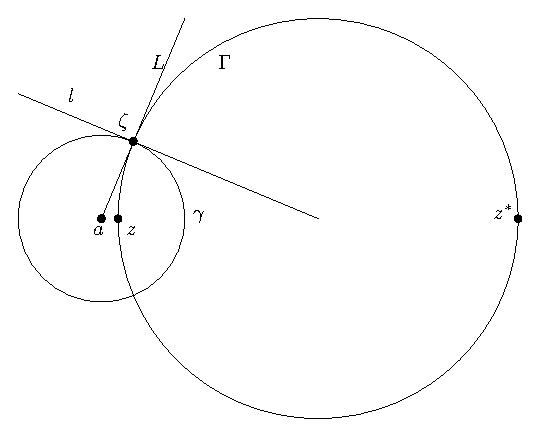
\includegraphics[scale=0.75]{neob.eps}
        \label{fig:23.1}
    \end{figure}
    Пусть $L$~--- касательная к $\Gamma$ из $a$, $\zeta \in L \cap \Gamma$.
    Тогда
    \begin{align*}
      & \left| a - \zeta \right|^2 = \left| a-z \right|\cdot \left| a-z^* \right| = R^2
    \end{align*}
    а значит, $\zeta \in \gamma$. Пусть $l$~--- касательная к $\Gamma$ в точке
    $\zeta$, $l \perp [a;\zeta] \Rightarrow l \perp L$.
    \item Достаточность.
    \begin{itemize}
        \item $\Gamma$~--- прямая, тогда $a \in \Gamma$, и значит, $z$ и $z^*$
        принадлежат одной полупрямой, исходящей из центра.
        \\
        Если точки лежат по разные стороны от центра, то построим окружность
        $\Gamma_1$ диаметром $zz^*$; тогда угол между $z$, точкой пересечения и
        $z^*$ равен $90^{\circ}$, а угол между $a$, точкой пересечения и центром
        окружности острый, т.~е. $L$ и $l$ не перпендикулярны).
            \begin{figure}[h!]
        \centering
        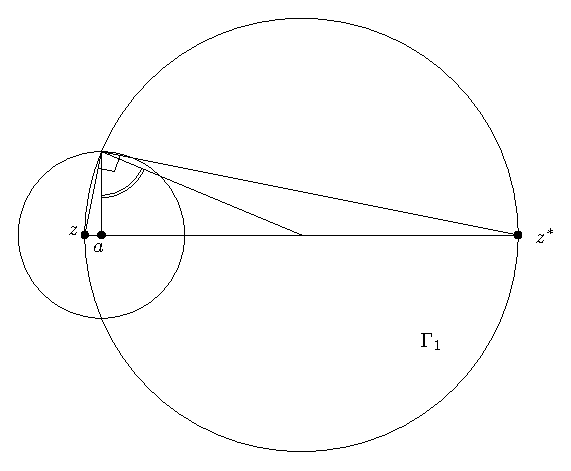
\includegraphics[scale=0.75]{dok.eps}
        \label{fig:23}
    \end{figure}
        \item $\Gamma$~--- окружность, тогда пусть $\zeta \in \Gamma \cap
        \gamma$, тогда
        \begin{align*}
          & \left| a - \zeta \right|^2 = \left| a-z \right|\cdot \left| a-z^* \right| = R^2
        \end{align*}
    \end{itemize}
\end{itemize}
\pr (теоремы)
$z$, $z^*$ симметричны относительно $\gamma$ (пусть окружности). Пусть $f$~---
ДЛО \eqref{(23.1)}, \eqref{(23.2)}. Пусть $w = f(z)$, $w^* = f(z^*)$, нужно
доказать, что они симметричны относительно $\tilde{\gamma} = f(\gamma)$.
\\
Рассмотрим $w$, $w^*$. Пусть $\tilde{\Gamma}$~--- любая окружность или прямая,
такая, что $w, w^* \in \tilde{\Gamma}$. Значит, по круговому свойству существует
окружность или прямая $\Gamma$: $\tilde{\Gamma} = f(\Gamma)$. По свойству
однолистности $z, z^* \in \Gamma$. Значит, по лемме $1$ $\gamma \perp \Gamma$.
Тогда, по свойству сохранения углов, $\tilde{\Gamma} \perp \tilde{\gamma}$. По
лемме $1$ тогда $w$ и $w^*$ симметричны относительно $\tilde{\Gamma}$.
\theorem
Множество ДЛО образует группу отображений относительно операции суперпозиции.
\pr
~
\begin{itemize}
    \item Очевидно, существует единичный элемент~--- тождественное отображение.
    \item У каждого ДЛО существует и единственно обратное ДЛО (см. теорему $1$).
    \item Суперпозиция ДЛО есть ДЛО. Действительно, пусть
    \begin{align*}
      & \zeta = \frac{a_1z+b_1}{c_1z+d_1}, \ w = \frac{a_2z+b_2}{c_2z+d_2}, \ a_1d_1 - c_1d_1 \neq 0, \ a_2d_2 - b_2c_2 \neq 0
    \end{align*}
    Положим
    \begin{align*}
      & z = \frac{z_1}{z_2}, \ \zeta = \frac{\zeta_1}{\zeta_2}, \ w = \frac{w_1}{w_2}
    \end{align*}
    Тогда
    \begin{align*}
      & \left( \begin{matrix}
              \zeta_1 \\
              \zeta_2
          \end{matrix} \right) = \left( \begin{matrix}
              a_1 & b_1 \\
              c_1 & d_1
          \end{matrix} \right) \cdot \left( \begin{matrix}
              z_1 \\
              z_2
          \end{matrix} \right), \ \left( \begin{matrix}
              w_1 \\
              w_2
          \end{matrix} \right) = \left( \begin{matrix}
              a_2 & b_2 \\
              c_2 & d_2
          \end{matrix} \right) \cdot \left( \begin{matrix}
              \zeta_1 \\
              \zeta_2
          \end{matrix} \right)
    \end{align*}
    \begin{align*}
      & \left( \begin{matrix}
              w_1 \\
              w_2
          \end{matrix} \right) = \left( \begin{matrix}
              a_2 & b_2 \\
              c_2 & d_2
          \end{matrix} \right) \cdot \left( \begin{matrix}
              a_1 & b_1 \\
              c_1 & d_1
          \end{matrix} \right) \cdot \left( \begin{matrix}
              z_1 \\
              z_2
          \end{matrix} \right)
    \end{align*}
    Получили невырожденное ДЛО.
\end{itemize}
\Example
Отобразить с помощью ДЛО области (см. рис.)
\begin{figure}[h!]
    \begin{minipage}[c]{0.45\textwidth}
        \centering
        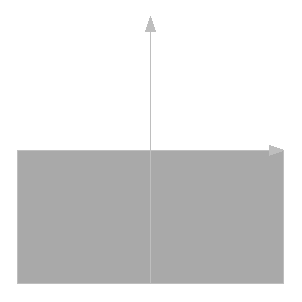
\includegraphics[scale=0.5]{half_plane.eps}
    \end{minipage}
    \begin{minipage}[c]{0.1\textwidth}
        \centering
        \LARGE{$\mapsto$}
    \end{minipage}
    \begin{minipage}[c]{0.45\textwidth}
        \centering
        
\includegraphics[scale=0.5]{round.eps}
    \end{minipage}
    \label{fig:23.2}
    \caption{$\Img z > 0 \mapsto \left| z \right| < 1$}
\end{figure}
\nonum
Возьмем любую $z_0: \ \Img z_0 > 0$. Пусть $z_0 \mapsto 0$, а $\ol{z_0} \mapsto
\infty$.
\\
Тогда
\begin{align*}
    & w = A\frac{z-z_0}{z-\ol{z_0}}
\end{align*}
Отыщем теперь $A$. Граница отображается на границу. Возьмем $x \in \RR$, она
должна отображаться на единичную окружность. Тогда
\begin{align*}
    & 1 = \abs{w} = \abs{A\frac{x-z_0}{x-\ol{z_0}}} = \left| A \right| \Rightarrow A = e^{i\alpha}
\end{align*}
Итак,
\begin{equation}\label{(23.6)}
    w = e^{i \alpha}\frac{z-z_0}{z-\ol{z_0}}
\end{equation}
\Example
Отобразить с помощью ДЛО области (см. рис.).
\\
\begin{figure}[h!]
    \begin{minipage}[c]{0.45\textwidth}
        \centering
        
\includegraphics[scale=0.5]{round.eps}
    \end{minipage}
    \begin{minipage}[c]{0.1\textwidth}
        \centering
        \LARGE{$\mapsto$}
    \end{minipage}
    \begin{minipage}[c]{0.45\textwidth}
        \centering
        
\includegraphics[scale=0.5]{round.eps}
    \end{minipage}
    \label{fig:23.3}
    \caption{$\left| z \right| < 1 \mapsto \left| z \right| < 1$}
\end{figure}
\nonum
Возьмем произвольную $z_0$ и отобразим ее в ноль; тогда симметричная $z_0^* =
\dst \frac{1}{\ol{z_0}}$ перейдет в $\infty$.
\\
Тогда
\begin{align*}
    & w = A\frac{z-z_0}{z-\dst \frac{1}{\ol{z_0}}} = \tilde{A}\frac{z-z_0}{1 - z\ol{z_0}}
\end{align*}
Граница перейдет в границу, а значит,
\begin{align*}
    & 1 = \abs{w} = \abs{\tilde{A}\frac{e^{i \varphi}-z_0}{1 - e^{i \varphi}\ol{z_0}}} = \abs{\tilde{A}\frac{e^{i \varphi}-z_0}{e^{-i \varphi}-\ol{z_0}}} = \abs{\tilde{A}}
\end{align*}
Итак,
\begin{equation}\label{(23.7)}
    w = e^{i \alpha}\frac{z-z_0}{1 - z\ol{z_0}}
\end{equation}
\Example
Отобразить с помощью ДЛО три различные точки $z_1, z_2, z_3$ в три точки $w_1,
w_2,w_3$.
\nonum
Заметим, что условиям удовлетворяет отображение вида
\begin{equation}\label{(23.8)}
    h(z) = \frac{z-z_1}{z-z_2} \cdot \frac{z_3-z_2}{z_3-z_1} = \frac{w-w_1}{w-w_2} \cdot \frac{w_3-w_2}{w_3-w_1} = g(w)
\end{equation}
\begin{align*}
  & w = f(z) = g^{-1}(h(z))
\end{align*}
Существование получено. Докажем единственность.
\\
Пусть для начала $f(z_k) = z_k$, тогда
\begin{align*}
  & \frac{az_k + b}{cz_k+d} = z_k
\end{align*}
\begin{align*}
  & cz^2_k + (d-a)z_k - b = 0
\end{align*}
Значит, поскольку квадратное уравнение имеет три решения, все его коэффициенты
равны нулю. Значит, $f(z) = z$.
\\
Пусть существуют $f_1(z)$, $f_2(z)$, причем $f_1(z_k) = f_2(z_k) = w_k$; тогда
$z_k = f_1^{-1}(f_2(z_k))$, тогда по групповому свойству $f_1^{-1}(z) =
f_2^{-1}(z)$, а значит, $f_1(z) = f_2(z)$.
\Example
Отобразить с помощью ДЛО области (см. рис.).
\\
\begin{figure}[h!]
    \begin{minipage}[c]{0.45\textwidth}
        \centering
        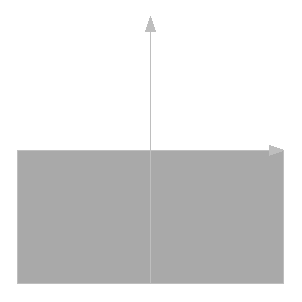
\includegraphics[scale=0.5]{half_plane.eps}
    \end{minipage}
    \begin{minipage}[c]{0.1\textwidth}
        \centering
        \LARGE{$\mapsto$}
    \end{minipage}
    \begin{minipage}[c]{0.45\textwidth}
        \centering
        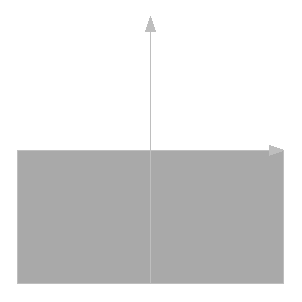
\includegraphics[scale=0.5]{half_plane.eps}
    \end{minipage}
    \label{fig:23.4}
    \caption{$\Img z > 0 \mapsto \Img z > 0$}
\end{figure}
\nonum
Пусть $x_1, x_2, x_3 \in \RR$, $x_1 < x_2 < x_3$, $u_1, u_2, u_3 \in \RR$, $u_1
< u_2 < u_3$, построим отображение $f(x_k) = u_k$. по примеру $3$ такое
отображение существует и единственно, границу оно переводит в границу. Из
свойства сохранения углов следует сохранение ориентации границы. Рассматривая
\eqref{(23.8)}, получаем все действительные  коэффициенты, т.~е. $a, b, c, d \in
\RR$, тогда $\forall x \in \RR \ \argm w'(x) = 0 \Rightarrow w'(x) > 0$, т.~е.
\begin{align*}
  & w'(x) = \frac{ad-cb}{(cx+d)^2} > 0 \Leftrightarrow ad-cb > 0
\end{align*}
Итак, необходимо и достаточно, чтобы все коэффициенты ДЛО были действительны,
причем $ad-cb > 0$.
\section{$\S 24.$ Конформные отображения элементарными функциями. Теорема Римама.}
Рассмотрим функции, обладающие локальной однолистностью.
\begin{center}
    \textbf{Степенная функция}
\end{center}
Фиксируем $t > 0$, рассмотрим область $G = \CC \setminus [0;+\infty)$. Пусть
\begin{align*}
  & w = \left| z \right|^t \exp(it \argt z), \ \argt z \in (0, 2 \pi)
\end{align*}
Функция регулярна при любом $t$. Действительно,
\begin{align*}
  & h(z) = \ln \left| z \right| + i \argt_0 z
\end{align*}
регулярна на этой области, а
\begin{align*}
  & w = \exp(t h(z))
\end{align*}
регулярна в этой области, как суперпозиция регулярных функций.
\\
Исследуем теперь однолистность. Рассмотрим
\begin{align*}
  & G_{0,\varphi_0} = \left\{ z \mid \left| z \right| > 0, \ \argt z \in (0; \varphi_0)\right\}
\end{align*}
\begin{align*}
  & l_{\varphi} = \left\{ z \mid z = r e^{i \varphi}, \ r > 0, \ \varphi \in (0, \varphi_0)\right\}
\end{align*}
Тогда
\begin{align*}
  & w(l_\varphi) = \left\{ w \mid w = \rho e^{i t \varphi}, \ \rho > 0 \right\}
\end{align*}
Тогда условие однолистности:
\begin{align*}
  & \begin{cases}
      0 < \varphi_0 < 2 \pi \\
      0 < t \varphi_0 < 2 \pi
  \end{cases}
\end{align*}
Значит, функция конформна на этой области.
\Example
$t = 2$, $w = z^2$.
\\
Условие однолистности: $\varphi_0 \in (0; \pi)$.
\begin{figure}[h!]
    \begin{minipage}[c]{0.45\textwidth}
        \centering
        
\includegraphics[scale=0.5]{half_round.eps}
    \end{minipage}
    \begin{minipage}[c]{0.1\textwidth}
        \centering
        \LARGE{$\mapsto$}
    \end{minipage}
    \begin{minipage}[c]{0.45\textwidth}
        \centering
        
\includegraphics[scale=0.5]{cut_rnd.eps}
    \end{minipage}
    \label{fig:24.1}
\end{figure}
\\
Заметим, что данный полукруг содержится в $G_{0, \pi}$~--- области
однолистности, значит, функция будет однолистна.
\Example
$t = 2$, $w = z^2$.
\\
Условие однолистности: $\varphi_0 \in (0; \pi)$.
\begin{figure}[h!]
    \begin{minipage}[c]{0.45\textwidth}
        \centering
        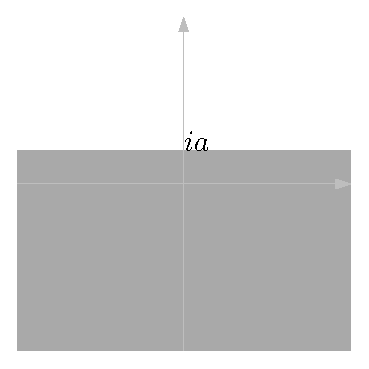
\includegraphics[scale=0.5]{top.eps}
    \end{minipage}
    \begin{minipage}[c]{0.1\textwidth}
        \centering
        \LARGE{$\mapsto$}
    \end{minipage}
    \begin{minipage}[c]{0.45\textwidth}
        \centering
        
\includegraphics[scale=0.5]{parabola.eps}
    \end{minipage}
    \label{fig:24.2}
\end{figure}
\\
Заметим, что данная полуплоскость содержится в $G_{0, \pi}$~--- области
однолистности, значит, функция будет однолистна. Зная, что граница переходит в
границу, отыщем $w(x+ia)$.
\begin{align*}
  & w(x+ia) = (x+ia)^2 = x^2 - a^2 + 2ixa
\end{align*}
\begin{align*}
  & \begin{cases}
      u = x^2 - a^2 \\
      v = 2xa
  \end{cases} \Rightarrow u  = \left( \frac{v}{2a} \right)^2 - a^2
\end{align*}
Поскольку $0$ не лежит в полуплоскости, искомая область будет внешностью
параболы.
\Example
$w = \left| z \right|^{\frac{1}{2}}\exp \left(\dst \frac{i}{2}\argt z\right)$.
\begin{figure}[h!]
    \begin{minipage}[c]{0.45\textwidth}
        \centering
        
\includegraphics[scale=0.5]{parabola.eps}
    \end{minipage}
    \begin{minipage}[c]{0.1\textwidth}
        \centering
        \LARGE{$\mapsto$}
    \end{minipage}
    \begin{minipage}[c]{0.45\textwidth}
        \centering
        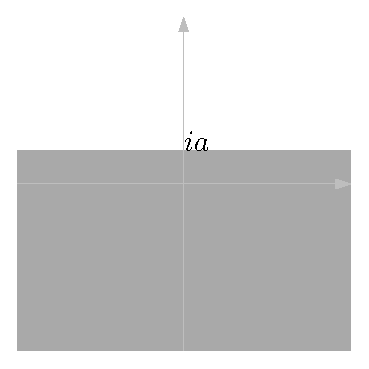
\includegraphics[scale=0.5]{top.eps}
    \end{minipage}
    \label{fig:24.3}
\end{figure}
Обратное к примеру $2$ отображение.
\begin{center}
    \textbf{Экспонента}
\end{center}
Всюду регулярна, но для однолистности необходимо, чтобы не было отличающихся на
$2 i \pi$ элементов (в силу периодичности).
\begin{figure}[h!]
    \centering
    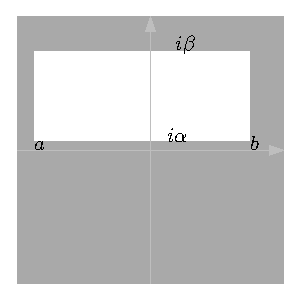
\includegraphics[scale=0.75]{odn_exp.eps}
    \label{fig:24.4}
    \caption{Область однолистности экспоненты}
\end{figure}
\begin{align*}
  & \begin{cases}
      -\infty \leq a \leq b \leq \infty \\
      0 \leq \beta - \alpha < 2 \pi
  \end{cases}
\end{align*}
\Example
\begin{figure}[h!]
    \begin{minipage}[c]{0.45\textwidth}
        \centering
        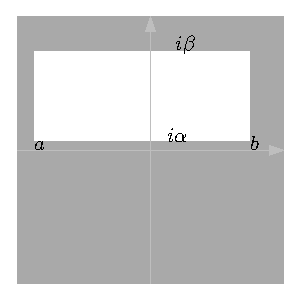
\includegraphics[scale=0.75]{odn_exp.eps}
    \end{minipage}
    \begin{minipage}[c]{0.1\textwidth}
        \centering
        \LARGE{$\mapsto$}
    \end{minipage}
    \begin{minipage}[c]{0.45\textwidth}
        \centering
        
\includegraphics[scale=0.5]{obraz_exp.eps}
    \end{minipage}
    \label{fig:24.5}
\end{figure}
Пусть $z = x+iy_0$, фиксированный $y_0 \in (\alpha,\beta)$. Тогда $\forall x \in
(a,b)$
\begin{align*}
  & f(z) = te^{iy_0}, \ t \in \left( e^{a}, e^{b} \right)
\end{align*}
\Example
~
\\
\begin{figure}[h!]
    \begin{minipage}[c]{0.45\textwidth}
        \centering
        
\includegraphics[scale=0.5]{polupolosa.eps}
    \end{minipage}
    \begin{minipage}[c]{0.1\textwidth}
        \centering
        \LARGE{$\mapsto$}
    \end{minipage}
    \begin{minipage}[c]{0.45\textwidth}
        \centering
        
\includegraphics[scale=0.5]{half_round.eps}
    \end{minipage}
    \label{fig:24.6}
    \caption{Перевод полуполосы в полуокружность.}
\end{figure}
Вертикальная черта переходит в полуокружность, верхняя граница~--- в отрезок
$[-1;0]$, нижняя граница~--- в отрезок $[0;1]$.
\Example
~
\\
\begin{figure}[h!]
    \begin{minipage}[c]{0.45\textwidth}
        \centering
        
\includegraphics[scale=0.5]{d_polupol.eps}
    \end{minipage}
    \begin{minipage}[c]{0.1\textwidth}
        \centering
        \LARGE{$\mapsto$}
    \end{minipage}
    \begin{minipage}[c]{0.45\textwidth}
        \centering
        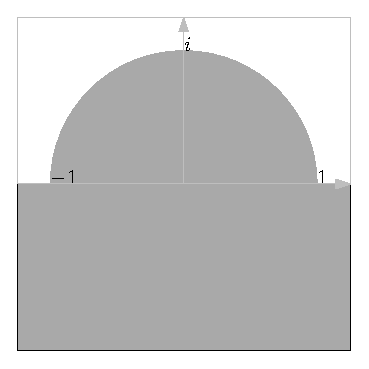
\includegraphics[scale=0.5]{out_rnd.eps}
    \end{minipage}
    \label{fig:24.7}
    \caption{Перевод полуполосы во внешность полуокружности.}
\end{figure}

    \begin{flushright}
    \textit{Лекция 19 (от 09.11)}
\end{flushright}
\begin{center}
    \textbf{Функция Жуковского}
\end{center}
\begin{equation}\label{(24.1)}
    w = \frac{1}{2}\left( z+\frac{1}{z} \right)
\end{equation}
Заметим, что $0$ и $\infty$~--- полюсы $1$ порядка, $\pm 1$~--- нули
производной.
\\
В каждой точке $z \not \in \left\{0, \pm 1,\infty \right\}$ функция конформна. В
точке $0$
\begin{align*}
  & g(z) = \frac{1}{w(z)} = \frac{2z}{z^2+1}
\end{align*}
Эта функция в нуле регулярна и имеет ненулевую производную, а значит, конформна
в нуле. В точке $\infty$
\begin{align*}
  & \varphi(z) = w\left( \frac{1}{z} \right) = \frac{1}{2}\left( \frac{1}{z} + z \right)
\end{align*}
Заметим, что это та же $w$, и в силу конформности в нуле конформна и на
бесконечности. В остальных точках проверим однолистность.
\begin{align*}
  & \frac{1}{2}\left( z_1 + \frac{1}{z_1} \right) - \frac{1}{2}\left( z_1 + \frac{1}{z_1} \right) = 0
\end{align*}
\begin{align*}
  & (z_1-z_2) \left( 1-\frac{1}{z_1z_2} \right)
\end{align*}
\begin{align*}
  & \left[ \begin{matrix}
          z_1=z_2 \\
          z_1z_2 = 1
      \end{matrix} \right.
\end{align*}
Область однолистности $G$: $\pm 1 \not \in G$, $\forall z \in G \ \dst
\frac{1}{z} \not \in G$.
\Example
Функция $w = \dst \frac{1}{z}$ задает две симметрии: относительно единичной
окружности и относительно действительной оси. Соответственно, области
однолистности:
\begin{itemize}
    \item $\left| z \right| < 1$
    \item $\left| z \right| > 1$
    \item $\Img z > 0$
    \item $\Img z < 0$
\end{itemize}
Пусть $z = e^{i \varphi}$, тогда функция Жуковского:
\begin{align*}
  & w = \frac{1}{2}\left( e^{i \varphi} + e^{-i\varphi}\right)
\end{align*}
\begin{equation}\label{(24.2)}
    \begin{cases}
        u = \frac{1}{2}\left( r+\frac{1}{r} \right)\cos \varphi \\
        v = \frac{1}{2}\left( r-\frac{1}{r} \right)\sin \varphi
    \end{cases}
\end{equation}
\Example
~
\begin{itemize}
    \item Пусть задана окружность
    \begin{align*}
      \gamma_r = \left\{ z: \left| z \right| = r, \ r \neq 1\right\}
    \end{align*}
    \begin{align*}
      & \frac{u^2}{a^2} + \frac{v^2}{b^2} = 1, \ a = \frac{1}{2}\left( r + \frac{1}{r} \right), \ b = \frac{1}{2}\left|  r - \frac{1}{r} \right|
    \end{align*}
    \begin{align*}
      & a^2+b^2 = c^2 = 1
    \end{align*}
    Такая окружность переходит в эллипс с фокусами в $\pm 1$, действительной
    полуосью $a$ и мнимой $b$.
    \item Пусть задан луч
    \begin{align*}
      l_\varphi = \left\{ z \mid z = re^{i\varphi}, \ r > 0\right\}, \ \varphi \in [-\pi;\pi) \setminus \left\{ 0, \pm \frac{\pi}{2}, -\pi \right\}
    \end{align*}
    \begin{equation}\label{(24.3)}
        \frac{u^2}{\cos^2 \varphi} - \frac{v^2}{\sin^2\varphi} = 1
    \end{equation}
    Такой луч переходит в гиперболу с фокусами в $\pm 1$.
    \begin{itemize}
        \item $\varphi \in \left( 0; \dst \frac{\pi}{2} \right)$~--- отображение
        в правую ветвь гиперболы, движение по ней вверх.
        \item $\varphi \in \left(\dst \frac{\pi}{2}; \pi \right)$~---
        отображение в левую ветвь гиперболы, движение по ней вверх.
        \item $\varphi \in \left( - \dst \frac{\pi}{2}; 0 \right)$~---
        отображение в правую ветвь гиперболы, движение по ней вниз.
        \item $\varphi \in \left( -\pi; -\dst \frac{\pi}{2} \right)$~---
        отображение в левую ветвь гиперболы, движение по ней вниз.
    \end{itemize}
\end{itemize}
\Example
~
\\
\begin{figure}[h!]
    \begin{minipage}[c]{0.45\textwidth}
        \centering
        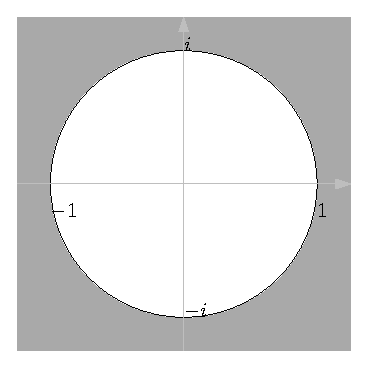
\includegraphics[scale=0.75]{rnd_in.eps}
    \end{minipage}
    \begin{minipage}[c]{0.1\textwidth}
        \centering
        \LARGE{$\mapsto$}
    \end{minipage}
    \begin{minipage}[c]{0.45\textwidth}
        \centering
        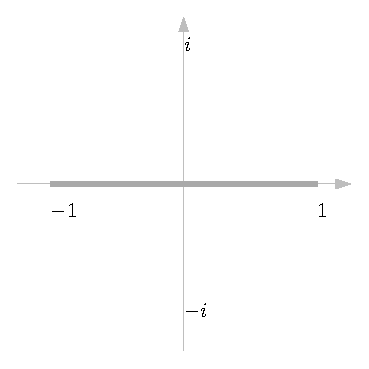
\includegraphics[scale=0.5]{pm1.eps}
    \end{minipage}
    \label{fig:24.10}
    \caption{Перевод единичного круга в $\CC \setminus [-1;1]$}
\end{figure}
\FloatBarrier
\Example
~
\\
\begin{figure}[h!]
    \begin{minipage}[c]{0.45\textwidth}
        \centering
        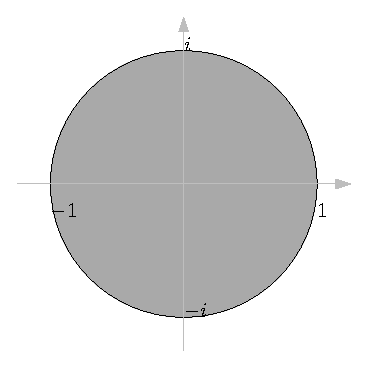
\includegraphics[scale=0.75]{rnd_out.eps}
    \end{minipage}
    \begin{minipage}[c]{0.1\textwidth}
        \centering
        \LARGE{$\mapsto$}
    \end{minipage}
    \begin{minipage}[c]{0.45\textwidth}
        \centering
        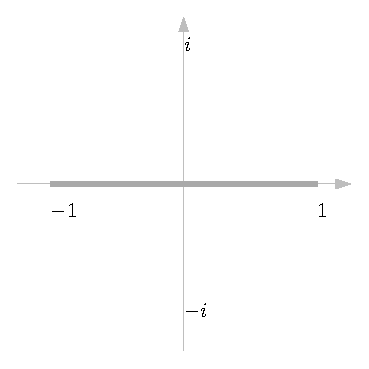
\includegraphics[scale=0.5]{pm1.eps}
    \end{minipage}
    \label{fig:24.11}
    \caption{Перевод внешности единичного круга в $\CC \setminus [-1;1]$}
\end{figure}
\FloatBarrier
\Example
~
\\
\begin{figure}[h!]
    \begin{minipage}[c]{0.45\textwidth}
        \centering
        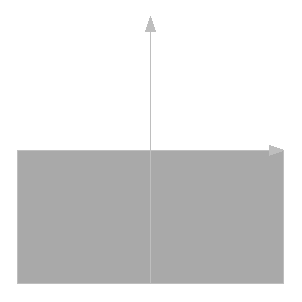
\includegraphics[scale=0.75]{half_plane.eps}
    \end{minipage}
    \begin{minipage}[c]{0.1\textwidth}
        \centering
        \LARGE{$\mapsto$}
    \end{minipage}
    \begin{minipage}[c]{0.45\textwidth}
        \centering
        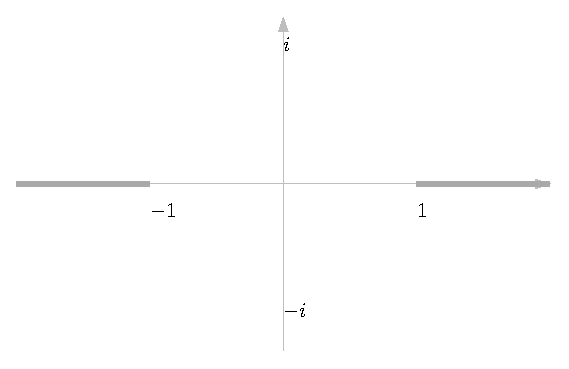
\includegraphics[scale=0.5]{pm1out.eps}
    \end{minipage}
    \label{fig:24.12}
    \caption{Перевод верхней полуплоскости в $\CC \setminus ((-\infty;-1]\cup[1;+\infty)$}
\end{figure}
\FloatBarrier
\Example
~
\\
\begin{figure}[h!]
    \begin{minipage}[c]{0.45\textwidth}
        \centering
        
\includegraphics[scale=0.75]{half_plane_t.eps}
    \end{minipage}
    \begin{minipage}[c]{0.1\textwidth}
        \centering
        \LARGE{$\mapsto$}
    \end{minipage}
    \begin{minipage}[c]{0.45\textwidth}
        \centering
        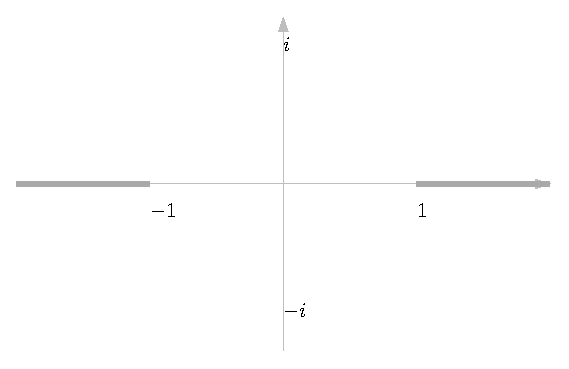
\includegraphics[scale=0.5]{pm1out.eps}
    \end{minipage}
    \label{fig:24.13}
    \caption{Перевод нижней полуплоскости в $\CC \setminus ((-\infty;-1]\cup[1;+\infty)$}
\end{figure}
\FloatBarrier
Отыщем обратную функцию Жуковского.
\begin{align*}
  & w = \frac{1}{2}\left( z+\frac{1}{z} \right) \Rightarrow z^2 - 2wz + 1 = 0
\end{align*}
\begin{align*}
  & z = w \pm g(w), \ g(w) \in \sqrt{w^2-1}
\end{align*}
\Example
Ветвь обратной функции Жуковского, где $g \sim w$ при $w \to \infty$, $z = w -
g(w)$, выполняет следующее преобразование:
\\
\begin{figure}[h!]
    \begin{minipage}[c]{0.45\textwidth}
        \centering
        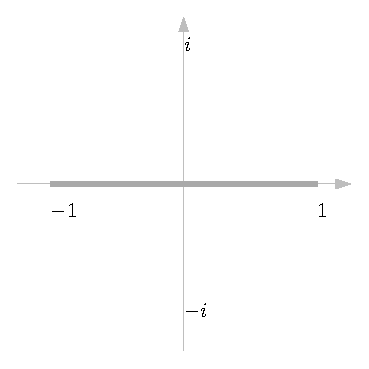
\includegraphics[scale=0.5]{pm1.eps}
    \end{minipage}
    \label{fig:24.14}
    \begin{minipage}[c]{0.1\textwidth}
        \centering
        \LARGE{$\mapsto$}
    \end{minipage}
        \begin{minipage}[c]{0.45\textwidth}
        \centering
        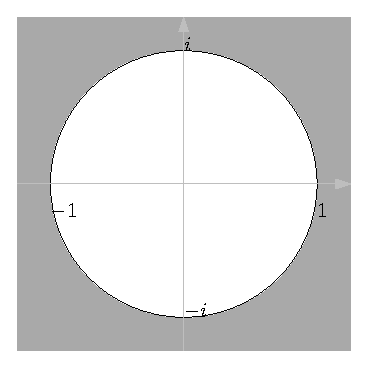
\includegraphics[scale=0.75]{rnd_in.eps}
    \end{minipage}
    \caption{Перевод $\CC \setminus [-1;1]$ в единичный круг}
\end{figure}
\FloatBarrier
\Example
Ветвь обратной функции Жуковского, где $g \sim w$ при $w \to \infty$, $z = w +
g(w)$, выполняет следующее преобразование:
\\
\begin{figure}[h!]
        \begin{minipage}[c]{0.45\textwidth}
        \centering
        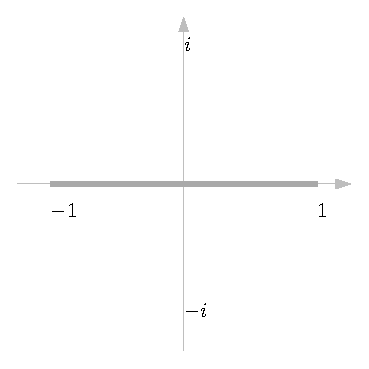
\includegraphics[scale=0.5]{pm1.eps}
    \end{minipage}
    \begin{minipage}[c]{0.1\textwidth}
        \centering
        \LARGE{$\mapsto$}
    \end{minipage}
        \begin{minipage}[c]{0.45\textwidth}
        \centering
        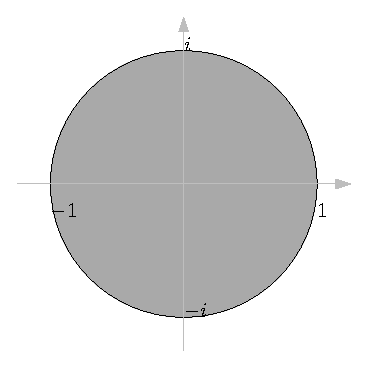
\includegraphics[scale=0.75]{rnd_out.eps}
    \end{minipage}
    \label{fig:24.15}
    \caption{Перевод $\CC \setminus [-1;1]$ во  внешность единичного круга}
\end{figure}
\FloatBarrier
\Example
Ветвь обратной функции Жуковского, где $g(0) = i$, $z = w - g(w)$, выполняет
следующее преобразование:
\\
\begin{figure}[h!]
        \begin{minipage}[c]{0.45\textwidth}
        \centering
        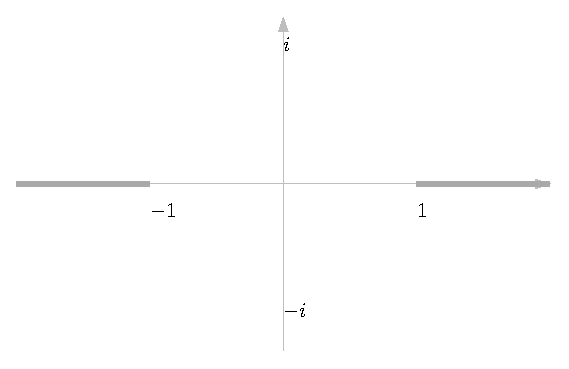
\includegraphics[scale=0.5]{pm1out.eps}
    \end{minipage}
    \begin{minipage}[c]{0.1\textwidth}
        \centering
        \LARGE{$\mapsto$}
    \end{minipage}
    \begin{minipage}[c]{0.45\textwidth}
        \centering
        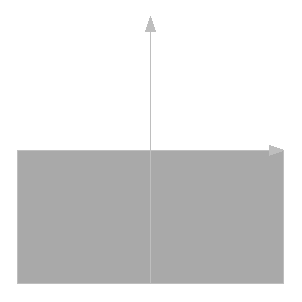
\includegraphics[scale=0.75]{half_plane.eps}
    \end{minipage}
    \label{fig:24.16}
    \caption{Перевод $\CC \setminus (-\infty;-1]\cup[1;+\infty)$ в верхнюю полуплоскость}
\end{figure}
\FloatBarrier
\Example
Ветвь обратной функции Жуковского, где $g(0) = i$, $z = w + g(w)$, выполняет
следующее преобразование:
\\
\begin{figure}[h!]
        \begin{minipage}[c]{0.45\textwidth}
        \centering
        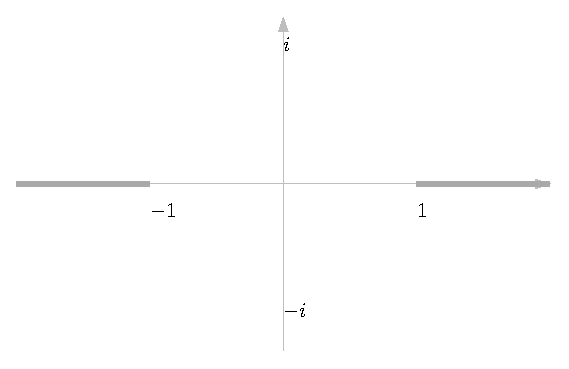
\includegraphics[scale=0.5]{pm1out.eps}
    \end{minipage}
    \begin{minipage}[c]{0.1\textwidth}
        \centering
        \LARGE{$\mapsto$}
    \end{minipage}
    \begin{minipage}[c]{0.45\textwidth}
        \centering
        
\includegraphics[scale=0.75]{half_plane_t.eps}
    \end{minipage}
    \label{fig:24.17}
    \caption{Перевод $\CC \setminus (-\infty;-1]\cup[1;+\infty)$ в нижнюю полуплоскость}
\end{figure}
\FloatBarrier
\begin{center}
    \textbf{Теорема Римана}
\end{center}
$\CC$ нельзя конформно отобразить на единичный круг. Действительно, функция (в
предположении существования) будет ограничена, регулярна (в силу определенности
на всей комплексной плоскости она обязана быть целой), значит, по теореме
Лиувилля это константа, что не является требуемым отображением.
\theorem
Общий вид конформного отображения $B_1(0) \mapsto B_1(0)$:
\begin{equation}\label{(24.4)}
    f(z) = e^{i\beta}\frac{z-a}{1-z\ol{a}}
\end{equation}
\pr
Если $f$ удовлетворяет \eqref{(24.4)}, то $f: B_1(0) \mapsto B_1(0)$ есть ДЛО, а
значит, оно конформно.
\\
Пусть теперь $g: B_1(0) \mapsto B_1(0)$~--- некоторое конформное отображение.
Докажем, что такая функция удовлетворяет \eqref{(24.4)}.
\\
Заметим:
\begin{align*}
  \exists w_0 \in B_1(0): \ g(0) = w_0
\end{align*}
Расмотрим теперь
\begin{align*}
  h(w) = \frac{w-w_0}{1-w\ol{w_0}}, \ h(w_0) = 0, \ h:B_1(0)\mapsto B_1(0)
\end{align*}
Положим
\begin{align*}
  f(z) = h(g(z))
\end{align*}
$f$ регулярна, как суперпозиция регулярных функций, и причем $f(0) = 0$,
$f:B_1(0) \mapsto B_1(0)$. Тогда по лемме Шварца $\forall z \in B_1(0) \ \left|
    f(z) \right|\leq \left| z \right|$.
\\
Тогда $f^{-1}$ таже будет регулярна, $f^{-1}(0) = 0$, $f^{-1}: B_1(0) \mapsto
B_1(0)$. Тогда по лемме Шварца $\forall w \in B_1(0) \ \left| f^{-1}(w)
\right|\leq \left| w \right|$. Подставляя сюда $w = f(z)$, получим $\left| z
\right| \leq \left| f(z) \right|$, т.~е. $\left| z \right| = \left| f(z)
\right|$, и по лемме Шварца выполняется $f(z) = e^{i\alpha}z$.
\\
Тогда $g(z)$~--- ДЛО. Проверим, что $g$ имеет вид \eqref{(24.4)}.
\begin{align*}
& e^{i\alpha}z = h^{-1}(g(z)); \ \exists z_0 \in B_1(0): \ g(z_0) = 0
\end{align*}
\begin{align*}
& e^{i\alpha} = (h^{-1})'(0)(g'(z_0)) = \frac{g'(z_0)}{h'(w_0)}
\end{align*}
\begin{align*}
& \alpha \in \Arg g'(z_0) - \Arg h'(w_0)
\end{align*}
\begin{align*}
& h'(w_0) = \left.\frac{1-w\ol{w_0}+\ol{w_0}(w-w_0)}{(1-w\ol{w_0})^2}\right|_{w=w_0} = 1 - \left| w_0 \right|^2 > 0 \Rightarrow 0 \in \Arg h'(w_0)
\end{align*}
\begin{align*}
& \alpha \in \Arg g'(z_0)
\end{align*}
Рассмотрим теперь 
\begin{align*}
& g_1(z) = e^{i\alpha}\frac{z-z_0}{1-z\ol{z_0}}
\end{align*}
\begin{align*}
&\varphi(z) = g(g_1^{-1}(w)): B_1(0) \mapsto B_1(0)
\end{align*}
\begin{align*}
&\varphi(g_1(z)) = g(w), \ \varphi(0) = 0, \ \Arg \varphi'(0) + \Arg g_1'(0) = \Arg g'(z_0)
\end{align*}
Дифференцируя,
\begin{align*}
& \alpha \in \Arg g_1(0), \ 0 \in \Arg \varphi'(0)
\end{align*}
По лемме Шварца для прямой и обратной функций
\begin{align*}
& \left| \varphi(z) \right| = \left| z \right| \Rightarrow \varphi(z) = z
\end{align*}
(в силу $0 \in \Arg \varphi'(0)$). Но тогда $g_1(z) = g(z)$, и теорема
доказана.
\lemma 
Пусть область $G\subseteq \CC$ такова, что существует конформное $f_0: G \mapsto
B_1(0)$. Тогда любое конформное отображение $G$ на $B_1(0)$ имеет вид
\begin{align*}
  & f(z) = h(f_0(z))
\end{align*}
причем $h$ имеет вид \eqref{(24.4)}.
\pr
Пусть $f_1: G \mapsto B_1(0)$~--- конформное. Рассмотрим 
\begin{align*}
  & \varphi(w) = f_1(f_0^{-1}(w)): B_1(0) \mapsto B_1(0)
\end{align*}
Оно конформно как суперпозиция конформных. По теореме $1$ это ДЛО,
уловлетворяющее \eqref{(24.4)}. Поскольку
\begin{align*}
& f_1(z) = \varphi(f_0(z))
\end{align*}
то лемма доказана.
\theorem (единственности конформных отображений)
Пусть $G$ такова, что существует конформное $f_0:G \mapsto B_1(0)$. Тогда
множество всех конформных отображений $G \mapsto B_1(0)$ зависит от трех
действительных параметров. В частности, такое отображение единственно, если
выполнены условия:
\begin{equation}\label{(24.5)}
f(z_0) = 0, \ \argt f'(z_0) = \alpha \in [0;2\pi), \ z_0 \in G
\end{equation}
\pr
Из леммы $1$ и теоремы $1$ следует утверждение о трех параметрах.
\\
Докажем теперь единственность. Допустим, от противного, существуют $f_1$, $f_2$,
удовлетворяющие \eqref{(24.5)}. Пусть
\begin{align*}
  & \varphi(w) = f_1(f_2^{-1}(w)), \ \varphi(f_2(z)) = f_1(z), \ \varphi(0) = 0
\end{align*}
Значит, $\varphi(z)$ будет ДЛО по лемме $1$. Дифференцируя в $z_0$, имеем
\begin{align*}
    & \argt \varphi'(0) + \Arg f_2'(z_0) = \Arg f_1'(z_0)
\end{align*}
\begin{align*}
  & 0 \in \Arg \varphi'(0) \Rightarrow \varphi(0) = 0, \ z_0 = 0, \ \alpha = 0
\end{align*}
\begin{align*}
  & \varphi(z) = z \Rightarrow f_1(z) = f_2(z)
\end{align*}
\theorem (Римана)
Пусть $G$~--- область в $\CCC$, граница которой содержит более одной точки.
Тогда существует конформное $f: G \mapsto B_1(0)$.
\corollary
Если $G_1 \subseteq \CCC$, $G_2 \subseteq \CCC$, и ганицы каждой содержат более
одной точки, то существует конформное обображение $G_1$ на $G_2$.
\pr
Пусть $f_1: G_1 \mapsto B_1(0)$, $f_2: G_2 \mapsto B_1(0)$, тогда искомое
отображение $\varphi(z) = f_1(f_2^{-1}(z)): G_1 \mapsto G_2$.
\theorem (принцип соответствия границ)
Пусть $G_1, G_2$~--- ограниченные односвязные области в $\CC$ с кусочно гладкими
границами $\Gamma_1, \Gamma_2$. Пусть $f: G_1 \mapsto G_2$~--- конформное; тогда
существует непрерывное продолжение $\tilde{f}$ такое, что оно отображает
$\Gamma_1$ на $\Gamma_2$ с сохранением ориентации.
    \begin{flushright}
    \textit{Лекция 20 (от 10.11)}
\end{flushright}
\section{$\S 25.$ Принцип симметрии.}
\theorem
Пусть заданы области $G$, $G^*$ в верхней полуплоскости с кусочно гладкими
границами $\Gamma$, $\Gamma^*$. Пусть границы содержат конечное чило интервалов
действительной оси $l_1, \dots, l_n$, $l_1^*, \dots, l_n^*$. Пусть $\tilde{G}$,
$\tilde{G^*}$~--- симметричные относительно действительной оси области. Пусть
$f: G \cup \dst \bigcup_{s=1}^n l_s \mapsto G^*\cup \dst \bigcup_{s=1}^n l_s^*$
конформна на $G$ и непрерывна на $G \cup \dst \bigcup_{s=1}^n l_s$ взамно
однозначно отображает $\forall s \in \left\{ 1, \dots, n \right\} \ l_s \mapsto
l_s^*$. Тогда существует (аналитическое) продолжение $f$ на область $G \cup \dst
\bigcup_{s=1}^n l_s \cup \tilde{G}$, конформно отображающее ее на $G^* \cup \dst
\bigcup_{s=1}^n l_s^* \cup \tilde{G^*}$.
\begin{figure}[h!]
    \begin{minipage}[c]{0.5\textwidth}
        \centering
        
\includegraphics[scale=0.75]{1st.eps}
    \end{minipage}
    \begin{minipage}[c]{0.5\textwidth}
        \centering
        
\includegraphics[scale=0.75]{2nd.eps}
    \end{minipage}
    \label{fig:25.1}
\end{figure}
\pr
Зададим функцию $F$ (искомое продолжение).
\begin{equation}\label{(25.1)}
    F(z) = \begin{cases}
        f(z), \ z \in G \cup \bigcup_{s=1}^n l_s \\
        \ol{f(\ol{z})}, \ z \in \tilde{G}
    \end{cases}
\end{equation}
Докажем дифференцируемость. Пусть $z_0 \in \tilde{G}$; тогда
\begin{align*}
  & \exists \varepsilon > 0: \ \forall \Delta z: \ \left| \Delta z \right| < \varepsilon \ z_0+\Delta z \in G
\end{align*}
\begin{align*}
  & \frac{F(z_0+\Delta z) - F(z_0)}{\Delta z} = \frac{\ol{f}(\ol{z_0+\Delta z}) - \ol{f}(\ol{z_0})}{\Delta z} = \ol{\frac{f(\ol{z_0}+\ol{\Delta z}) - f(\ol{z_0})}{\ol{\Delta z}}}
\end{align*}
Тогда
\begin{align*}
  & \ol{z_0} \in G, \ \ol{z_0} +\ol{\Delta z} \in G, \ \exists f'(\ol{z_0}) = \lim_{\Delta z \to 0} \frac{f(\ol{z_0}+\ol{\Delta z}) - f(\ol{z_0})}{\ol{\Delta z}}
\end{align*}
\begin{align*}
  & \exists F'(z_0) = \ol{f'(\ol{z_0})}
\end{align*}
Пусть теперь $x_0 \in l_s$. Докажем, что $F(z)$ непрерывна в $x_0$. Рассмотрим
нижний полукруг окрестности.
\begin{align*}
  & \lim_{z \os{\tilde{G}}{\to} x_0}F(z) = \lim_{\ol{z} \os{G}{\to} x_0}\ol{f(\ol{z})} = \ol{\lim_{\ol{z} \os{G}{\to} x_0}f(\ol{z})} = \ol{f(x_0)} = f(x_0) \in l_s^*
\end{align*}
Аналогично находится предел по верхнему полукругу.
\\
Тогда по теореме о стирании разреза $F(z)$ регулярна в $x_0$ и, значит,
регулярна во всей объединенной области.
\\
Докажем, наконец, однолистность. Область $G$ отображалась однолистно, как и
интервалы; каждая точка $\tilde{G}$ соответствует единственной точке $G$, как и
$\tilde{G^*}$ и $G^*$, а значит, отображение однолистно и на оставшейся части.
\corollary
принцип симметрии можнообобщить на симметрии относительно любой прямой или
окружности.
\pr
Всякую такую кривую можем перевести в действительную ось (область~--- в верхнюю
полуплоскость), применить принцип симметрии и перевести обратно.
\Example
Найти преобразование, переводящее данные области.
\begin{figure}[h!]
    \begin{minipage}[c]{0.45\textwidth}
        \centering
        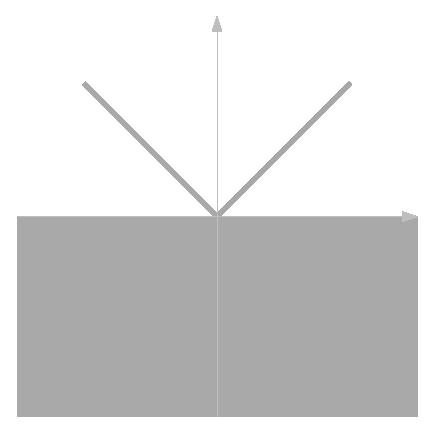
\includegraphics[scale=0.75]{ex24_1.eps}
    \end{minipage}
    \begin{minipage}[c]{0.1\textwidth}
        \centering
        \LARGE{$\mapsto$}
    \end{minipage}
    \begin{minipage}[c]{0.45\textwidth}
        \centering
        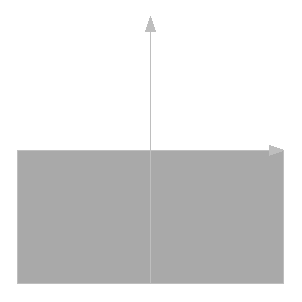
\includegraphics[scale=0.5]{half_plane.eps}
    \end{minipage}
    \label{fig:25.1}
\end{figure}
Воспользовавшись принципом симметрии, рассмотрим лишь правую часть вместе с
мнимой осью. Используя $w_1 = z^4$, получим $\CC \setminus[-4;+\infty)$, причем
функция будет непрерывно продлена на нижний край разреза от нуля и до
бесконечности. Применяя $w_2 = w_1+4$, получим $\CC \setminus[0;+\infty)$, причем
функция будет непрерывно продлена на нижний край разреза от $4$ и до
бесконечности. При помощи $w_3 = \sqrt{\left| w_2 \right|}\exp \left(
\dst \frac{i}{2}\argt w_2\right)$ получаем верхнюю полуплоскость, а $(-\infty;
-2]$ имеет непрерывное продолжение функции на себе. Затем сдвигаем этот разрез:
$w_4 = w_3+2$, и извлекаем корень: $w_5 = \sqrt{\left| w_4 \right|}\exp \left(
    \dst \frac{i}{2}\argt w_4\right)$. По принципу симметрии можем раскрыть все
до полуплоскости.
\begin{center}
    \begin{tabular}{cccc}
      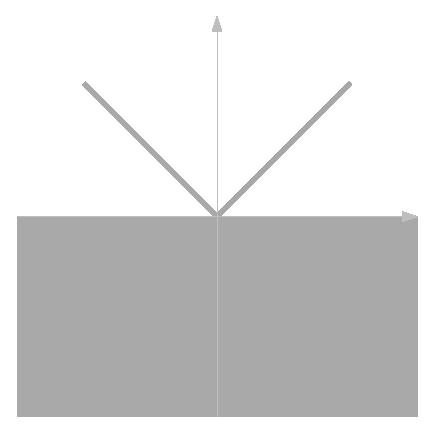
\includegraphics[scale=0.75]{ex24_1.eps} & $\Rightarrow$ & 
\includegraphics[scale=0.75]{2511.eps} & $\mapsto$ \\
    \end{tabular}
\end{center}
\begin{center}
    \begin{tabular}{cccc}
      \includegraphics[scale=0.75]{2512.eps} & $\mapsto$ & \includegraphics[scale=0.75]{2513.eps} & $\mapsto$ \\
    \end{tabular}
\end{center}
\begin{center}
    \begin{tabular}{cccc}
      \includegraphics[scale=0.75]{2514.eps} & $\mapsto$ & \includegraphics[scale=0.75]{2515.eps} & $\mapsto$ \\
    \end{tabular}
\end{center}
\begin{center}
    \begin{tabular}{cccc}
      \includegraphics[scale=0.75]{2516.eps} & $\Rightarrow$ & \includegraphics[scale=1]{half_plane.eps} & \\
    \end{tabular}
\end{center}
\Example
Найти преобразование, переводящее данные области.
\begin{align*}
  & G = \left\{ z = x+iy \mid y^2 < 2p \left( x+\frac{p}{2} \right) \right\}, \ p > 0
\end{align*}
\begin{figure}[h!]
    \begin{minipage}[c]{0.45\textwidth}
        \centering
        \includegraphics[scale=0.75]{2520.eps}
    \end{minipage}
    \begin{minipage}[c]{0.1\textwidth}
        \centering
        \LARGE{$\mapsto$}
    \end{minipage}
    \begin{minipage}[c]{0.45\textwidth}
        \centering
        \includegraphics[scale=0.5]{half_plane.eps}
    \end{minipage}
    \label{fig:25.1}
\end{figure}
Воспользовавшись принципом симметрии, рассмотрим лишь верхнюю часть вместе с
действительной осью. Используя $w_1 = \sqrt{\left| z \right|}\exp \left(\dst
    \frac{i}{2}\argt z\right)$, получаем полуполосу. Растянем эту полуполосу при
помощи $w_2 = \pi\sqrt{\frac{2}{\pi}}$, экспонентой $w_3 = e^{w_2}$ превратим в
верхнюю полуплоскость с вырезанным единичным полукругом. Функцией Жуковского
$w_4 = dst \frac{1}{2}\left( w_3+\dst\frac{1}{w_4} \right)$ переводим в верхнюю
полуплоскость, но она имеет особый участок $[-1;+\infty)$. По принципу симметрии
можем раскрыть это до плоскости с разрезом по $(-\infty;-1]$, и легко, сдвигая
$w_5 = -w_4+1$ и извлекая корень $w_6 = \sqrt{\left| w_5 \right|}\exp \left(\dst
    \frac{i}{2}\argt w_5\right)$, получаем искомое.
\begin{center}
    \begin{tabular}{cccc}
      \includegraphics[scale=0.75]{2520.eps} & $\Rightarrow$ & \includegraphics[scale=0.75]{2521.eps} & $\mapsto$ \\
    \end{tabular}
\end{center}
\begin{center}
    \begin{tabular}{cccc}
      \includegraphics[scale=0.75]{2522.eps} & $\mapsto$ & \includegraphics[scale=0.75]{2523.eps} & $\mapsto$ \\
    \end{tabular}
\end{center}
\begin{center}
    \begin{tabular}{cccc}
      \includegraphics[scale=0.75]{2524.eps} & $\mapsto$ & \includegraphics[scale=0.75]{2525.eps} & $\Rightarrow$ \\
    \end{tabular}
\end{center}
\begin{center}
    \begin{tabular}{cccc}
      \includegraphics[scale=0.75]{2526.eps} & $\mapsto$ & \includegraphics[scale=1]{2527.eps} & $\mapsto$ \\
    \end{tabular}
\end{center}
\begin{center}
    \begin{tabular}{cccc}
      \includegraphics[scale=0.5]{half_plane.eps} & & & \\
    \end{tabular}
\end{center}
\section{$\S 26.$ Задача Дирихле на плоскости.}
\theorem
Пусть $f: G \mapsto D$ регулярная и непрстоянная. Пусть $\tilde{u}: D \mapsto
\RR$ гармоническая. Тогда $u(z) = \tilde{u}(f(z))$ также гармоническая.
\pr
Пусть $z_0 \in G$~--- произвольная точка. Пусть $f(z_0) = w_0$, и $f(G) =
G^*$~--- также, как известно, область. Тогда
\begin{align*}
  & \exists \varepsilon > 0: B_\varepsilon(w_0) \subseteq G^* \subseteq D
\end{align*}
По теореме $2$ $\S 4$
\begin{align*}
  & \exists h(w): \ \Real h(w) = \tilde{u}(w), \ w \in B_\varepsilon(w_0)
\end{align*}
причем $h$~--- регулярная. Рассмотрим теперь $h(f(z))$ в окрестности
$B_\delta(w_0)$, такой, чо $f\left( B_\delta(z_0) \right) \subseteq
B_\varepsilon(w_0)$. Тогда в этой окрестности $h$ будет регулярной,
$\tilde{u}(w) = \Real h(w)$~--- гармонической, тогда и $u(z) = \tilde{u}(f(z))$
тоже будет гармонической в этой окрестности, а в силу произвольности выбора
$z_0$~--- и на всей области.
\Def
\textbf{Классическим решением задачи Дирихле в области $G$} называется
следующее:
\begin{itemize}
    \item $G$~--- ограниченная односвязная область в $\CC$ с кучочно гладкой
    границей $\Gamma$;
    \item дана непрерывная функция $u_0(z)$ на этой границе;
    \item нужно найти гармоническую функцию $u(z)$ в области $G$, непрерывную на
    ее замыкании и удовлетворяющую условию: $u\Big|_\Gamma = u_0$.
\end{itemize}
\Def
\textbf{Общей задачей Дирихле} называется следующее:
\begin{itemize}
    \item $G$~--- односвязная область в $\CCC$ с кучочно гладкой границей $\Gamma$;
    \item дана непрерывная функция всюду за исключением коненого числа точек
    разрыва $1$ рода $\zeta_1, \dots, \zeta_n$ $u_0(z)$ на этой границе и
    ограниченная на ней за вычетом этих точек;
    \item нужно найти гармоническую функцию $u(z)$ в области $G$, ограниченную
    на ее замыкании, непрерывную на ее замыкании за вычетом этих точек и
    удовлетворяющую условию: $u = u_0$ на границе за вычетом этих точек.
\end{itemize}
\lemma
Лемма доказывается для случая ограниченной области.
\\
Пусть $G$~--- ограниченная односвязная область в $\CC$. Если решение общей
задачи Дирихле существует в этой области с $u_0(z)$ и $\tilde{\Gamma} = \Gamma
\setminus \dst \bigcup_{k=1}^n \left\{ \zeta_k \right\}$, то все значения $u(z)$
лежат на отрезке $\left[ m, M \right]$, где $m = \us{z \in\tilde{\Gamma}}{\inf} u_0(z)$, $M = \us{z \in\tilde{\Gamma}}{\sup}u_0(z)$.
\pr
Пусть $d = \sup \left| z_1-z_2 \right|$, $z_1, z_2 \in G$~--- диаметр множества.
Пусть
\begin{equation}\label{(26.1)}
    U_\varepsilon = M + \varepsilon \sum_{k=1}^n \ln \frac{d}{\left| z-\zeta_k\right|}, \ \varepsilon > 0
\end{equation}
Это гармоническая функция, причем она не меньше $M$ и непрерывна на замыкании
за вычетом точек разрыва, причем
\begin{equation}\label{(26.2)}
    \lim_{z \to \zeta_k} U_\varepsilon(z) = \infty
\end{equation}
Полагая
\begin{align*}
  & \gamma_r^k = \left\{ z \in G: \left| z - \zeta_k \right| = r\right\}
\end{align*}
\begin{equation}\label{(26.3)}
    \lim_{r \to 0}\min \left\{ U_\varepsilon(z) \mid z \in \gamma_r^k \right\} = +\infty
\end{equation}
\begin{align*}
    & \forall z \in \tilde{\Gamma} \ U_\varepsilon(z) > M\geq u_0(z) = u(z)
\end{align*}
Из ограниенности и выполнимости \eqref{(26.3)} для $u(z)$ имеем, чтопри
достаточно малых $r$ на границе области $G_r = G \setminus \dst \bigcup_{k=1}^n
B_r(\zeta_k)$ $U_\varepsilon(z) > U(z)$. По принципу максмума гармонической
функции это соотношение верно и для всей $G_r$.
\\
Фиксируем произвольную  $z \in G$. тогда $\exists r_0: z \in G_{r_0}$, значит,
$U_\varepsilon(z) > u(z)$ на всей $G$. При устремлении $\varepsilon$ к нулю
получаем, что $u(z) \leq M$.
\\
Аналогично можем ограничить сверху гармоническую $-u(z)$ числом $-m$ и получить
искомое.
\Note
Без условия ограниченности области лемма также справедлива.
\corollary
Для случая непостоянной $u_0(z)$ выполняются строгие неравенства.
\pr
От противного: предположим существование внутренней точки области, где $M$
достигается; тогда должна существовать $z_1 \in G: \ u(z_1) > M$ (аналогичнно
доказательству принципа максимума). Противоречие с неравенством, даже нестрогим.    

    \begin{flushright}
    \textit{Лекция 21 (от 16.11)}
\end{flushright}
\theorem
В общей задаче Дирихле при существовании решения в ограниченной области онобудет
единственным. Решение ищем как ограниченную функцию.
\pr
От противного. Допустим, существуют два различных решения $u_1$, $u_2$. Тогда $w
= u_1-u_2 : G \mapsto \RR$, $\Delta w = 0$, $w\Big|_\Gamma = 0$. Тогда по лемме
$1$ $w \equiv 0$.
\Note
Условие ограниченности области является лишь техническим. Условие же
ограниченности функции на области существенно.
\Example
\begin{align*}
  & u(x,y) = \frac{x^2+y^2-2x}{x^2+y^2}
\end{align*}
\begin{align*}
  & G = \left\{ (x,y) \mid x^2+y^2<2x \right\} = \left\{ z: \left| z \right| <1\right\}
\end{align*}
При граничном условии~--- нуле эта функция является решением задачи Дирихле, но
и тождественный нуль также решение. При условии ограниченности эта функция не
подходит.
\begin{center}
    \textbf{Класическая задача Дирихле в круге $B_R(0), \ R > 0$}
\end{center}
\begin{equation}\label{(26.4)}
    \begin{cases}
        \Delta u = 0, \ \left| z \right|< R \\
        u \big|_{\left| z \right| = R} = u_0(z)
    \end{cases}
\end{equation}
причем $u_0(z)$ непрерывна на $\gamma_r$ и решение \eqref{(26.4)} непрерывно на
некотором $B_{R_1}(0), \ R_1 > R$.
\\
Тогда существует регулярная $f: B_{R_1}(0) \mapsto \CC$, что $\Real f(z) =
u(z)$. Тогда по интегральной формуле Коши
\begin{align*}
  & \forall z \in B_R(0) \ f(z) = \frac{1}{2 i \pi} \int_{\gamma_R} \frac{f(\zeta)}{\zeta - z}d\zeta = \frac{1}{2 \pi} \int_{0}^{2\pi} \frac{f(Re^{i\psi})\zeta(\psi)}{\zeta(\psi) - z}d\psi
\end{align*}
Введем теперь симметричную точку $z^* = \dst \frac{R^2}{z}$. Тогда
\begin{align*}
  & \frac{1}{2 i \pi} \int_{\gamma_R} \frac{f(\zeta)}{\zeta - z^*}d\zeta = \frac{1}{2 \pi} \int_{0}^{2\pi} \frac{f(Re^{i\psi})\zeta(\psi)}{\zeta(\psi) - z^*}d\psi = 0
\end{align*}
\begin{align*}
  & f(z) = \frac{1}{2\pi}\int_{0}^{2\pi}f(\zeta(\psi))\left( \frac{\zeta(\psi)}{\zeta(\psi) - z} - \frac{\zeta(\psi)}{\zeta(\psi) - z^*}\right)d\psi = \frac{1}{2\pi}\int_{0}^{2\pi}f(\zeta(\psi))\left( \frac{\zeta(\psi)}{\zeta(\psi) - z} - \right. \\
  & \left. - \frac{\zeta(\psi)\ol{z}}{\zeta(\psi)\ol{\zeta(\psi)} - \zeta(\psi)\ol{z}}\right)d\psi = \frac{1}{2\pi}\int_{0}^{2\pi}f(\zeta(\psi))\left( \frac{\zeta(\psi)\ol{\zeta(\psi)} - z\ol{z}}{\left| \zeta(\psi) - z \right|^2}\right)d\psi = \frac{1}{2\pi}\int_{0}^{2\pi}f(\zeta(\psi))\cdot \\
  & \cdot \left( \frac{\abs{\zeta(\psi)}^2 - \abs{z}^2}{\left| \zeta(\psi) - z \right|^2}\right) d\psi = \frac{1}{2\pi}\int_{0}^{2\pi}f(Re^{i\psi})\left( \frac{R^2 - \abs{z}^2}{\left| Re^{i\psi} - z \right|^2}\right) d\psi
\end{align*}
\begin{equation}\label{(26.5)}
    u(z) = \frac{1}{2\pi}\int_{0}^{2\pi}\tilde{u}_0(\psi)\left( \frac{R^2 - \abs{z}^2}{\left| Re^{i\psi} - z \right|^2}\right) d\psi = \frac{1}{2\pi}\int_{0}^{2\pi}u_0(Re^{i\psi})\left( \frac{R^2 - \abs{z}^2}{\left| Re^{i\psi} - z \right|^2}\right) d\psi
\end{equation}
\eqref{(26.5)} называется \textbf{формулой Пуассона}, интеграл~---
\textbf{интегралом Пуассона}.
\begin{equation}\label{(26.6)}
    K(\zeta,z) = \frac{1}{2\pi} \frac{\abs{\zeta}^2 - \abs{z}^2}{\left| \zeta - z \right|^2}
\end{equation}
\eqref{(26.6)} называется \textbf{ядром (интеграла) Пуассона}.
\begin{equation}\label{(26.7)}
    u(z) = \int_{0}^{2\pi}\tilde{u}_0(\psi)K\left(Re^{i\psi},z\right) d\psi
\end{equation}
\begin{equation}\label{(26.8)}
    K(\zeta,z) = \Real\left( \frac{1}{2\pi} \frac{\zeta+z}{ \zeta - z }\right)
\end{equation}
\begin{align*}
  & f(z) = \frac{1}{2\pi}\int_{0}^{2\pi}\tilde{u}_0(\psi)\frac{\zeta+z}{\zeta-z}d\psi = \frac{1}{2i\pi}\int_{\gamma_R}u_0(\zeta)\frac{\zeta+z}{\zeta-z}\frac{d\zeta}{\zeta}
\end{align*}
\begin{equation}\label{(26.9)}
    u(z) = \Real \frac{1}{2i\pi}\int_{\gamma_R}u_0(\zeta)\frac{\zeta+z}{\zeta-z}\frac{d\zeta}{\zeta}
\end{equation}
\lemma
\begin{align*}
  &\forall z \in B_R(0) \ I(z) = \int_0^{2\pi}K(Re^{i\psi}, z) d\psi = 1
\end{align*}
\pr
\begin{align*}
  & I(z) = \Real I^*(z) = \Real \frac{1}{2\pi}\int_0^{2\pi}\frac{\zeta + z}{\zeta - z} d\psi = \Real \frac{1}{2\pi}\int_{\gamma_R}\frac{\zeta + z}{\zeta - z} \frac{d\zeta}{\zeta} = \Real \left( \us{z}{\res}g(\zeta) + \us{0}{\res}g(\zeta)\right) = \\
  & = \Real(2 - 1) = 1
\end{align*}
\lemma
Пусть $\delta \in \left( 0;\dst \frac{\pi}{2} \right)$, $\zeta_0 \in \gamma_R: \
\zeta_0 = Re^{i\psi_0}, \ \psi_0 \in [0;2\pi)$. Пусть
\begin{align*}
  & \gamma(0, \delta) = \left\{ \zeta \in \gamma_R \mid \zeta = Re^{i\psi}, \ \psi \in (\psi_0+\delta, \psi_0 +2\pi - \delta) \right\}
\end{align*}
Тогда
\begin{align*}
  & \lim_{z \os{B_R(0)}{\to} \zeta_0} \max_{\zeta \in \gamma(0;\delta)}K(\zeta, z) = 0
\end{align*}
\pr
\begin{align*}
  & K(\zeta,z) = \frac{1}{2\pi} \frac{R^2-\abs{z}}{ \abs{\zeta - z }^2}
\end{align*}
$\forall \varepsilon > 0$ рассмотрим $z \in B_\varepsilon(\zeta_0) \cap B_R(0)$;
тогда
\begin{align*}
  & \forall \zeta \in \gamma_R \ \exists \varepsilon > 0: \ \left| \zeta - \zeta_0 \right| = R\left| 1-e^{i(\psi_0-\psi)} \right| > \varepsilon_0, \ \left| z - \zeta_0 \right| < \frac{\varepsilon_0}{2}
\end{align*}
\begin{align*}
  & \forall \zeta \in \gamma_R \ \exists \varepsilon > 0: \ \left| \zeta - z \right| \geq \left| \zeta - \zeta_0 \right| - \left| \zeta_0 - z \right| > \frac{\varepsilon_0}{2}
\end{align*}
\begin{align*}
  & 0 \leq \lim_{z \os{B_R(0)}{\to} \zeta_0} \max_{\zeta \in \gamma(0;\delta)}K(\zeta, z) \leq \lim_{z \os{B_R(0)}{\to} \zeta_0}\frac{2}{\pi\varepsilon_0}\left( R^2-\left| z \right|^2 \right) = 0
\end{align*}
\theorem
Решение общей задачи Дирихле существует в круге $B_r(0)$ и описывается
интегралом Пуассона.
\pr
\begin{equation}\label{(26.10)}
    u(z) = \frac{1}{2\pi}\int_{0}^{2\pi}\tilde{u}_0(\psi)\left( \frac{R^2 - \abs{z}^2}{\left| Re^{i\psi} - z \right|^2}\right) d\psi
\end{equation}
Докажем гармоничность.
\begin{align*}
  & f(z) = \frac{1}{2\pi}\int_{0}^{2\pi}\tilde{u}_0(\psi)\frac{\zeta + z}{\zeta-z}d\psi, \ \zeta = Re^{i\psi}
\end{align*}
Пусть $z \in B_R(0)$, $z+\Delta z\in B_R(0)$. Тогда
\begin{align*}
  & \frac{f(z+\Delta z) - f(z)}{\Delta z} - \frac{1}{\pi}\int_{0}^{2\pi}\tilde{u}_0(\psi)\frac{\zeta}{(\zeta-z)^2}d\psi = \frac{1}{\pi}\int_{0}^{2\pi}\tilde{u}_0(\psi)\left( \frac{z+\Delta z + \zeta}{\zeta - \Delta z - z} + \frac{\zeta + z}{\zeta - z} - \frac{\zeta}{(\zeta-z)^2}\right) d\psi = \frac{1}{\pi}\int_{0}^{2\pi}\tilde{u}_0(\psi)\left( \frac{\zeta}{(\zeta - \Delta z - z)(\zeta - z)} - \frac{\zeta}{(\zeta-z)^2}\right) d\psi = \frac{1}{\pi}\int_{0}^{2\pi}\tilde{u}_0(\psi)\left( \frac{\zeta \Delta z}{(\zeta - \Delta z - z)(\zeta - z)^2}\right) d\psi \us{\Delta z \to 0} 0
\end{align*}
Производная существует, а значит, функция регулярна, а $u$ гармоническая.
\\
Докажем ограниченность. Из определения общей задачи Дирихле на границе за
вычетом конечного числа точек ограничена $u_0(z)$, а поскольку интеграл ядра
равен $1$, то и $u(z)$ ограничена тем же числом.
\\
Докажем непрерывность на границе. Для этого докажем, что
\begin{align*}
  & \lim_{z\os{B_R(0)}{\to} \zeta_0} u(z) = u(\zeta_0)
\end{align*}
Пусть
\begin{align*}
  &\Delta I=  \int_0^{2\pi}\tilde{u}_0(z)K(\zeta(\psi), z)d\psi - u_0(\zeta_0) = \int_0^{2\pi}(\tilde{u}_0-u_0(\zeta_0))K(\zeta(\psi), z)d\psi
\end{align*}
В силу непрерывности $u_0$ в $\zeta_0$
\begin{align*}
  & \forall \varepsilon > 0 \ \exists \delta > 0: \ \left| \psi - \psi_0 \right| < \delta \ \left| u_0(\zeta) - u_0(\zeta_0) \right| <\varepsilon, \ \zeta_0 = Re^{i\varphi_0}
\end{align*}
Положим
\begin{align*}
  & \gamma(1, \delta) = \left\{ \zeta \mid \zeta = Re^{i\psi}, \ \left| \psi - \psi_0 \right| < \delta \right\}, \ \gamma(0, \delta) = \gamma_R\setminus\gamma(1,\delta)
\end{align*}
\begin{align*}
  &\Delta I=  \int_{\psi_0-\delta}^{\psi_0+\delta}(\tilde{u}_0-u_0(\zeta_0))K(\zeta(\psi), z)d\psi + \int_{\psi_0+\delta}^{\psi_0+2\pi-\delta}(\tilde{u}_0-u_0(\zeta_0))K(\zeta(\psi), z)d\psi
\end{align*}
Первый интеграл ограничен сверху $\varepsilon$; для второго же по лемме $2$
$\exists \rho: \ \forall z \in B_\rho(z_0) \max_{\zeta \in
  \gamma(1,\delta)}K(\zeta,z) <\varepsilon$, а значит, модуль интеграла
ограничен сверху $4\pi M \varepsilon$. Значит, можем заметить, что предел
суммарного интеграла будет равен нулю.
\theorem
На ограниченной односвязной области $G$ с кусочно гладкой границей $\Gamma$
существует решение обобщенной задачи Дирихле.
\pr
По теореме Римана существует регулярная $f: G \mapsto B_1(0)$, конформная на
этой области. Тогда $\exists z=g(w): B_1(0) \mapsto G$, и это также конформное
отображение.
\\
То же верно и для замыканий по принципу соответствия границ. Пусть $f(\zeta) =
\alpha$, $g(\alpha) = \zeta$, $\left| \alpha \right|= 1$, $\zeta \in \Gamma$. В
исходной задаче Дирихле $u_0(\zeta)$ непрерына на границе за исключением
конечного числа точек $\tilde{u}(\alpha) = u(g(\alpha))$ обладает тем же
свойством на $\gamma_1$, и по теореме $3$ существует решение $u(w)$ задачи
Дирихле с граничным условием $\tilde{u}(\alpha)$. По формуле Пуассона
\begin{align*}
  & u(w) = \frac{1}{2i\pi}\int_{\gamma_1}\tilde{u}(\alpha)\frac{\alpha + w}{\alpha - w} \frac{d\alpha}{\alpha}
\end{align*}
$u(z) = u(f(z)): G \mapsto \RR$, эта функция гармоническая по теореме $1$, а на
границе $u(\zeta) = u_0(\zeta) = \tilde{u}(\alpha)$. Тогда
\begin{equation}\label{(26.11)}
    u(z) = \Real \frac{1}{2i\pi}\int_{\Gamma}u_0(\zeta)\frac{f(\zeta)+f(z)}{f(\zeta) - f(z)} \frac{f'(\zeta)d\zeta}{f(\zeta)}
\end{equation}
Заметим, что существует дробно-линейное отображение $\Img z > 0 \mapsto B_1(0)$.
Тогда, используя формулу \eqref{(26.11)}, получим теорему:
\theorem
Пусть $u_0(x)$ непрерывна на $\RR$ за исключением, быть может, конечного числа
точек разрыва первого рода, и ограничена. Тогда решение общей задачи Дирихле в
$\Img z > 0$ существует и описывается формулой
\begin{equation}\label{(26.12)}
    u(z) = \frac{1}{\pi}\int_{-\infty}^\infty \frac{y u_0(t)}{(x-t)^2 +y^2} dt, \ z = x+iy
\end{equation}

    \begin{flushright}
    \textit{Лекция 22 (от 17.11)}
\end{flushright}
\section{$\S 27.$ Аналитическое продолжение.}
\Def
Путь задана $f: D \mapsto \CC$, $D \subseteq G \subseteq \CC$, $G$~--- область,
$g: G \mapsto \CC$ регулярна. Если $\forall z \in D \ f(z) = g(z)$, то $g$
называется \textbf{аналитическим продолжением} $f$ на $G$.
\Example
\begin{align*}
  & e^x \to e^z = e^xe^{iy}, \ D = \RR \subseteq \CC \to G = \CC
\end{align*}
\Example
\begin{align*}
  & \sin x \to \sin z = \frac{e^{iz}-e^{-iz}}{2}, \ D = \RR \subseteq \CC \to \CC
\end{align*}
\Def
Пусть $a \in \CC$, $f: B_r(a) \mapsto \CC$, $r>0$~--- регулярная. Тогда $\left(
    B_r(a), f \right)$ называется \textbf{элементом аналитической функции с
  центром в точке $a$}.
\Def
Два элемента $\left( B_r(a), f \right)$ и $\left( B_\rho(b), g \right)$
называются \textbf{эквивалентными}, если $a = b$, $\forall z \in B_{r_0}(a) \
f(z) = g(z)$, $r_0 = \min \left\{ r, \rho \right\}$.
\Def
Пусть $\left( B_r(a), f \right)$~--- элемент аналитической функции, тогда
говорят, что элемент $\left( B_\rho(b), g \right)$ является его
\textbf{непосредственным аналитическим продолжением (НАП)}, если $B_r(a) \cap
B_\rho(b) \neq \varnothing$, $\forall z \in B_r(a) \cap B_\rho(b) \ f(z) =
g(z)$.
\Note
Если определены $B_r(a), B_\rho(b), f$, то по теореме единственности однозначно
определен и $\left( B_\rho(b), g \right)$.
\Def
Пусть $\left( B_r(a), f \right)$~--- элемент. Говорят, что $\left( B_\rho(b), g
\right)$ есть \textbf{аналитическое продолжение элемента $\left( B_r(a), f
  \right)$ вдоль конечной цепочки элементов (кругов)}, если $\exists \left\{
    \left( B_{r_k}(z_k), f_k \right) \right\}_{k=0}^n$ такое, что $\left(
    B_{r_0}(z_0), f_0 \right) \sim \left( B_r(a), f \right)$, $\left(
    B_{r_n}(z_n), f_n \right) \sim \left( B_\rho(b), g \right) $, $\forall k \in
\left\{ 1,\dots, n\right\}$ $\left( B_{r_k}(z_k), f_k \right)$ является
непосредственным аналитическим продолжением $\left( B_{r_{k-1}}(z_{k-1}),
    f_{k-1} \right)$.
\Example
\begin{align*}
  & f_1(z) = \sum_{n=0}^{\infty}z^n
\end{align*}
сходится на $B_1(0)$ и расходится при $\left| z \right| \geq 1$. Пусть $\left(
    B_1(0), f_1 \right)$~--- элемент; тогда
\begin{align*}
  & f_2 = \frac{1}{1-z}
\end{align*}
регулярна в $\CC \setminus \left\{ 1 \right\}$, и для $a \in \CC \setminus [1;
+\infty)$ элемент $\left( B_{\left| a-1 \right|}(a), f_2 \right)$ будет НАП
$\left( B_1(0), f_1 \right)$; для $a_2 \in (1; +\infty)$ элемент $\left(
    B_{\left| a_2-1 \right|}(a_2), f_2 \right)$ не будет НАП $\left( B_1(0), f_1
\right)$, но будет аналитическим продолжением вдоль конечной цепочи кругов.
\Example
Пусть
\begin{align*}
  & f_s(z) = \sqrt{\left| z \right|}\exp\left( \frac{i}{2}\argt_s(z) \right), \ \argt_s(z) \in \left( s-\frac{\pi}{2}, s+\frac{\pi}{2} \right)
\end{align*}
Для элемента $\left( B_1(1), f_0 \right)$ элемент $\left( B_1(i),
    f_{\frac{\pi}{2}} \right)$ будет НАП, а для него, в свою очередь, элемент
$\left( B_1(-1), f_\pi \right)$ будет НАП.
\\
Для элемента $\left( B_1(1), f_0 \right)$ элемент $\left( B_1(-i),
    f_{-\frac{\pi}{2}} \right)$ будет НАП, а для него, в свою очередь, элемент
$\left( B_1(-1), f_{-\pi} \right)$ будет НАП.
\begin{align*}
  & \forall z \in B_1(-1) \ f_\pi(z) = f_{-\pi}(z)
\end{align*}
\Def
Пусть $\left( B_r(a), f \right)$~--- элемент. Говорят, что $\left( B_\rho(b),g
\right)$ является \textbf{аналитическим продолжением вдоль кривой
  $\gamma_{ab}$}, если $\exists r > 0$, $\varphi:[0;l] \mapsto \CC$, $l$~---
длина кривой, $\gamma_{ab}: z = z(s)$, $s \in [0;l]$, а также существует
семейство элементов $\left\{ \left( B_r(z(s)), f(s) \right) \right\}_{s\in
  [0;l]}$, такое, что
\begin{itemize}
\item $\forall s_0 \in [0;l], \ \forall s \in [0;l]\cap [s_0-r; s_0 + r] \
\varphi(z) = f_{s_0}(z)$
\item $\left( B_r(a), f \right)\sim \left( B_r(z(0)), f_0 \right)$, $\left(
    B_\rho(b), g \right) \sim \left( B_r(z(l)), f_l \right)$
\end{itemize}
\Example
Можем рассмотреть те же элементы, что и в примере $4$, $s \in [0;\pi]$, и по
первой кривой $\gamma_1 = e^{is}$ придем к элементу $\left( B_1(e^{i\pi}),
    f_{\pi} \right)$, а по второй кривой $\gamma_2 = e^{-is}$ придем к элементу
$\left( B_1(e^{-i\pi}), f_{-\pi} \right)$.
\theorem
Аналитическое продолжение вдоль конечной цепочки и вдоль кривой эквивалентно.
\pr
По конечной цепочке построим кривую.
\\
По конечной цепочке элементов $\left\{ B_{r_k}(z_k), f_k \right\}$ построим
круги: для каждой точки $z \in [r_k; r_k+1]$ зададим $B_r(z)$, причем $0 <r \leq
\min \left\{ r_k \right\}$. Этот круг будет лежать в объединении исходных
кругов; тогда $\varphi(z) = f_k(z)$.
\\
По кривой построим конечную цепочку.
\\
Разобьем кривую на конечное число участков таких, что $\left| z(s_k) -
    z(s_{k-1}) \right|\leq \dst\frac{r}{2}$ и рассмотрим семейство $\left(
    B_r(z(s_k)), f_{s_k} \right)$. Тогда $z(s_{k})\in B_r(z(s_{k-1}))$,
пересечение непусто и функции на нем совпадают.
\Def
\textbf{Полной аналитической функцией, порожденной начальным элементом $\left(
      B_r(a), f \right)$}, называется совокупность всех аналитических
продолжений по всем кривым с началом в точке $a$, по которым оно возможно.
\Def
\textbf{Аналитической функцией, порожденной начальным элементом $\left(
      B_r(a), f \right)$}, называется связное семейство элементов полной
аналитической функции, начинающейся из этого элемента.
\\
\textbf{Связное семейство элементов}~--- такое семейство, где любые два элемента
могут быть получены один из другого, проходя только по этому семейству.
\theorem (о монодромии)
Пусть аналитическая функция $F(z)$ определена на односвязной области $G$ в
$\CC$. Тогда ее значения в любой точке этой области не зависят от кривой, по
которой получено аналитическим продолжением это значение.
\\
Говорят, что аналитическая функция, заданная на односвязной области, однозначна
в каждой точке и регулярна в области.
\section{$\S 28.$ Полные аналитические функции $\Ln z$, $\sqrt[n]{z}$ и римановы
  поверхности.}
$\forall a \neq 0$ рассмотрим $\left( B_{\left| a \right|}(a), h_a(z) \right)$,
$h_a(z)$~--- регулярная ветвь $\Ln z$ и $\left( B_{\left| a \right|}(a), g_a(z)
\right)$, $g_a(z)$~--- регулярная ветвь $\left\{ \sqrt[n]{z} \right\}$~---
\textbf{элементы, порожденные логарифмом и корнем}.
    \begin{flushright}
    \textit{Лекция 23 (от 23.11)}
\end{flushright}
\theorem
Пусть $a, b \in \CC \setminus \left\{ 0 \right\}$. Пусть $\left( B_{\left| a
      \right|}(a), h_a \right)$~--- элемент, порожденный $\Ln z$. Тогда для
любой $\gamma_{ab}$, не содержащей нуля, существует аналитическое продолжение в
некоторый элемент $\left( B_{\left| b \right|}(b), h_b \right)$~--- элемент,
порожденный $\Ln z$, причем
\begin{equation}\label{(28.1)}
    h_b(b) = h_a(a) + \int_{\gamma_{ab}}\frac{d\zeta}{\zeta}
\end{equation}
\begin{equation}\label{(28.2)}
    \forall z \in B_{\left| b \right|}(b) \ h_b(z) = h_b(b) + \int_{b}^z\frac{d\zeta}{\zeta}
\end{equation}
$\forall c \in \CC \setminus\left\{ 0 \right\}$, $\forall \left( B_{\left| c
      \right|}(c), h_c\right)$, порожденного $\Ln z$, существует
$\tilde{\gamma}_{ac}$ такая, что этот элемент есть аналитическое продолжение
исходного вдоль этой кривой.
\pr
Заметим, что в силу того, что кривая не содержит нуля, $d = \min \left\{ \left|
        \zeta \right|: \zeta \in \gamma_{ab} \right\} > 0$. Рассмотрим набор
точек $a = z_0, z_1, \dots, z_{K-1}, z_K = b$ на кривой, причем
$l_{\gamma_{z_{k-1}z_k}} \leq \dst \frac{d}{2}$. Зададим для каждой из точек шар
$B_{\left| z_k \right|}z_k$. Заметим, что $\left| z_k- z_{k-1} \right| \leq \dst
\frac{d}{2} < \left| z_{k-1} \right|$. Тогда, как видим, следующая точка лежит в
окрестности предыдущей.
\\
Допустим, доказано существование продолжения на $\gamma_{az_{k-1}}$; докажем
существование $\gamma_{az_k}$. На $B_{\left| z_k \right|}(z_k)$
\begin{equation}\label{(28.3)}
    h_k(z_k) = h_{k-1}(z_{k-1}) + \ln \left| z_k \right| - \ln \left| z_{k-1} \right| + i\Delta_{\gamma_{z_{k-1}z_k}} \argt z = h_{k-1}(z_{k-1}) +\int_{\gamma_{z_{k-1}z_k}} \frac{d\zeta}{\zeta}
\end{equation}
\begin{equation}\label{(28.4)}
    \forall z \in B_{\left| z_k \right|}(z_k) h_k(z) = h_k(z_k) + \int_{z_k}^z \frac{d\zeta}{\zeta}
\end{equation}
Значит, получили искомое продолжение.
\\
Для точки $c$ фиксируем некоторую не содержащую нуля кривую $\gamma_{ac}$. Для
нее существует аналитическое продолжение $\left( B_{\left| c \right|}(c),
    \tilde{h}_c \right)$; и $\exists k \in \ZZ: h_c(z) = \tilde{h}_c(z) + 2 i
\pi k$. Тогда искомая $\tilde{\gamma}_{ac}$ будет равна $\gamma_{ac}$,
объединенной с кругом с центром в нуле и радиусом $c$, обойденным $k$ раз.
\corollary
Полная аналитическая функция $\Ln z$ состоит из элементов $\left( B_{\left| a
      \right|}(a), h_a(z) + 2 i \pi k \right)$, $a \neq 0$, $k \in \ZZ$,
$h_a$~--- регулярная ветвь логарифма.
\begin{align*}
  & \left\{ \sqrt[n]{z} \right\} = \exp \left( \frac{1}{n}\Ln z \right)
\end{align*}
\corollary
Полная аналитическая функция $\left\{ \sqrt[n]{z} \right\}$ состоит из элементов
$\left( B_{\left| a \right|}(a), g_a(z)\exp \left( \frac{i}{n} 2 \pi k
    \right)\right)$, $a \neq 0$, $k \in \left\{ 0, \dots, n-1 \right\}$,
$g_a$~--- регулярная ветвь корня.
\begin{center}
    \textbf{Риманова поверхность $\Ln z$}
\end{center}
\begin{align*}
  & G_0 = \CC \setminus (-\infty; 0]: \ h_0(z) = \ln \left| z \right| + i \argm z, \ \argm z \in (-pi; \pi); \ h_k(z) = h_0(z) + 2 i \pi k, \ k \in \ZZ
\end{align*}
\begin{align*}
  & G_k = \CC \setminus (-\infty; 0]: \\
  & \forall x < 0 \ h_{k-1}(x+i0) = \ln \left| x \right| + i \pi + 2\pi (k-1)i, \  h_{k}(x+i0) = \ln \left| x \right| + i (-\pi) + 2\pi k i
\end{align*}
Значения на верхнем и нижнем краях разреза равны. Можем склеить верхнюю часть
$G_k$ с нижней $G_{k+1}$ для всех $k$. На этой поверхности функция будет
регулярна в любой точке.
\begin{center}
    \textbf{Риманова поверхность $\sqrt{z}$}
\end{center}
\begin{align*}
  & G_0 = \CC \setminus (-\infty; 0]: \ g_0(z) = \sqrt{\left| z \right|} \exp \left( \frac{i}{2} \argm z \right)
\end{align*}
\begin{align*}
  & G_1 = \CC \setminus (-\infty; 0]: \ g_1(z) = -g_0(z)
\end{align*}
\begin{align*}
  & \forall x < 0 \ g_0(x+i0) = i\sqrt{\left| x \right|}, \ g_0(x-i0) = -i\sqrt{\left| x \right|} \\
  & g_1(x+i0) = g_0(x-i0), \ g_1(x-i0) = -g_0(x+i0)
\end{align*}
Значения на верхнем и нижнем краях разреза равны. Можем склеить верхние части с
нижними. На этой поверхности функция будет регулярна в любой точке.
\section{$\S 29.$ Особые точки аналитических функций.}
\Def
Пусть аналитическая функция $F(z)$ такова, что $\exists \gamma_{ab}$: $\forall z
\in \gamma_{ab}\setminus \left\{ b \right\}$ есть аналитическое продолжение
вдоль $\gamma_{az}$, а вдоль $\gamma_{ab}$ его нет. Тогда $b$~--- \textbf{особая
  точка.}
\Def
Пусть $b = \infty$, при замене аргумента $\tilde{F}\left( \
dst \frac{1}{z}\right) = F(z)$ имеет особую точку в нуле, тогда $\infty$~---
\textbf{особая точка} функции $F$.
\Note
Полюса и СОТ регулярной функции~--- особые точки аналитической, а УОТ~--- нет.
\Def
Точка $a$ называется \textbf{точкой ветвления аналитической функции}, если
существует проколотая окрестность, где аналитическая функция определена, но не
однозначно, т.~е. можем в некоторой проколотой окрестности точки $a$ продолжить
функцию, обходя вокруг этой точки, до элемента с той же окрестностью, но другой
функцией.
\Example
$0, \infty$~--- точки ветвления логарифма (никогда не повторяются функции,
логарифмический порядок) и корня (могут повториться, алгебраический порядок).
\theorem (Коши-Адамара)
Пусть степенной ряд
\begin{align*}
  & \sum_{n=0}^\infty c_n(z-a)^n = S(z)
\end{align*}
сходится в круге $B_R(a), \ 0 < a < \infty$. Тогда на границе области (круга)
сходимости существуют особые точки аналитической функции.
\pr
От противного. Пусть $\gamma_R = \left\{ \zeta: \left| \zeta - a \right| = R
\right\}$,
\begin{align*}
  &\forall \zeta \in \gamma_R \ \exists \left( B_{r_\zeta}, f_\zeta \right), \ r_\zeta > 0
\end{align*}
аналитическое продолжение $\left( B_R(a), S(z) \right)$ вдоль радиуса
$\gamma_R$. Всю окружность можно покрыть кругами с центрами в каждой точке, и
существует конечное подпокрытие (лемма Гейне-Бореля), т.~е. конечный набор точек
$\left\{ \zeta_k \right\}_{k=1}^K$ таких, что круги с центрами в них содержат в
себе $\gamma_R$. Получили функцию (аналитическую):
\begin{align*}
  & F(z) = \begin{cases}
      \left( B_R(a), S(z) \right) \\
      \left( B_{r_k}(\zeta_k), f_k \right)
  \end{cases}
\end{align*}
Пусть $G$~--- объединение $B_R(a)$ и всех перечисленных кругов. Докажем
однозначность $F$ на $G$. Рассмотрим $m, n: \ B_{r_n}(\zeta_n)\cap
B_{r_m}(\zeta_m)\neq \varnothing$; тгда в пересечении этих двух кругов с
$B_R(a)$ $f_m(z) = S(z) = f_n(z)$, и по теореме единственности $f_n(z) = f_m(z)$
на пересечении этих двух кругов. Рассмотрим теперь $r = \inf \left\{ \left|
        z-\zeta \right| : z \in B_R(a), \ \zeta \in \CC \setminus G\right\} >
0$; тогда $B_{R+r} \subseteq G$ и $F(z)$ регулярна в этом круге. Ряд
\begin{align*}
  & \sum_{n=0}^\infty \frac{F^{(n)}(z)}{n!}(z-a)^n
\end{align*}
сходится к сумме при $\left| z-a \right|< R$, но тогда этот ряд и в круге
$B_{R+r}$ сходится, противоречие.
\Example
\begin{align*}
  & f(z) = \frac{1}{(z+3)(z^2+2)}
\end{align*}
Радиус сходимости равен $\sqrt{2}$.
\Example
\begin{align*}
  & \frac{1}{1-z} \sum_{n=0}^{\infty} z^n
\end{align*}
Одна особая точка на границе, расходится в них всех.
    \newpage
\section{Лекционные задачи.}
Автор решения многих задач: \href{https://vk.com/h0ho_haha}{Лев Нечитайло}.

\subsection{Различные системы множеств.}
\newpage
\lecture{1}{Различные системы множеств.}

В этом курсе имеется дело с функциями, аргументами которых являются множества.
\begin{definition}
	\mdef{Мерой} на множестве $X$ называется функция
	$\mu:\: \F \rightarrow [0,\, \infty]$, где $\F$~--- семейство подмножеств $X$.
\end{definition}

На $\F$ нужно наложить некоторые ограничения, потому как если, к примеру, определена мера для двух множеств,
то логично было бы, чтобы была определена мера и на их сумме, пересечении, объединении. Отсюда вытекают такие понятия как:

\begin{definition}
	Семейство $\F$ подмножеств множества $X$ (далее используется обозначение $\F \subset \mathcal{P} (X)\equiv 2^{X}$, где
	$\mathcal{P} (X)$~--- множество всех подмножеств множества $X$) называется \mdef{$\sigma$"=алгеброй}, если
	\begin{enumerate}[label=\arabic*\degree.]
		\item $\varnothing\in \F$.
		\item $\forall A,\, B\in\F:\: A\cap B\in\F,\,A\cup B\in\F,\, A\setminus B\equiv A\cap B^C\in\F$, где
		      $B^C=X\setminus B$.
		\item $X\in\F$.
		\item $\forall \{A_n\}_{n\in\N}\subset\F$ выполнено, что
		      $\bigcup\limits_{n=1}^{\infty}A_n\in\F,\,\bigcap\limits_{n=1}^{\infty}A_n\in\F$.
	\end{enumerate}
\end{definition}

\begin{definition}
	$\F$~--- \mdef{кольцо}, если выполняются условия $1\degree$ и $2\degree$.
\end{definition}
\begin{definition}
	$\F$~--- \mdef{алгебра}, если выполняются условия $1\degree$, $2\degree$ и $3\degree$.
\end{definition}

\begin{remark}
	Пусть $\F$~--- $\sigma$"=алгебра, тогда $\forall A\in\F:\: A^C=X\setminus A\in\F$. Тогда
	\[
		\bigcup\limits_{n=1}^{\infty}A_n=\left(\bigcup\limits_{n=1}^{\infty}A_n\right)^{CC}=
		\left(\bigcap\limits_{n=1}^{\infty}A_n^C\right)^C.
	\]
	Поэтому можно сказать, что вторая часть в условии $4\degree$ избыточна. Абсолютно аналогично и в обратную сторону,
	то есть эти два требования равносильны.
	\label{lect1remark1}
\end{remark}

\begin{remark}
	Пусть $\F$~--- кольцо,
	тогда $A\cap B=A\cap\left(B^{CC}\right)=A\setminus B^C=A\setminus\left(X\setminus B\right)=
		A\setminus\left(A\setminus B\right)$. То есть требование замкнутости по пересечению в свойстве $2\degree$ избыточно.
\end{remark}

\begin{exercise}
	Пусть $\F$~--- семейство всех ограниченных подмножеств множества $\R$. Тогда $\F$~--- кольцо, но не алгебра.
\end{exercise}

\begin{definition}
	Кольцо $\F$ называется
	\begin{enumerate}[label=\alph*)]
		\item \mdef{$\sigma$"=кольцом}, если $\forall \{A_n\}_{n=1}^{\infty}\subset\F$ выполнено, что
		      $\bigcup\limits_{n=1}^{\infty}A_n\in\F$.
		\item \mdef{$\delta$"=кольцом}, если $\forall \{A_n\}_{n=1}^{\infty}\subset\F$ выполнено, что
		      $\bigcap\limits_{n=1}^{\infty}A_n\in\F$.
	\end{enumerate}
\end{definition}

\begin{remark}
	Любое $\sigma$"=кольцо является $\delta$"=кольцом, но обратное неверно.
\end{remark}

\begin{definition}
	Множество $I\subset \R$ называется \mdef{промежутком}, если $\forall a,\, b\in I:\: [a,\, b]\subset I$.
	Промежуток $I$ называется \mdef{конечным}, если он ограничен.

	Например, $[a,\, b],\, (a,\, b),\, [a,\, b),\, (a,\, b]$~--- промежутки.
\end{definition}

Пусть $K_1$~--- семейство всех конечных промежутков на прямой. Легко заметить, что это не кольцо (объединение промежутков
--- не всегда промежуток). Отсюда вытекает новая структура:

\begin{definition}
	Семейство $\F\subset \mathcal{P} (X)$ называется \mdef{полукольцом}, если
	\begin{enumerate}[label=\arabic*\degree.]
		\item $\varnothing\in \F$.
		\item $\forall A,\, B\in\F:\: A\cap B\in\F$, а $A\setminus B$ представимо в виде
		      конечного дизъюнктного объединения элементов $\F$, то есть
		      \[\exists n\in\N: \: \exists A_1,A_2,\ldots,A_n\in\F: \: A\setminus B=\bigcup_{i=1}^{n}A_i
			      ,\, A_i\cap A_j=\varnothing,\, \forall i,j: i\neq j.\]
		      Если множества попарно не пересекаются, то вводиться обозначение:
		      \[A_1\cup A_2\cup\ldots\cup A_n=A_1\sqcup A_2\sqcup\ldots\sqcup A_n.\]
	\end{enumerate}
\end{definition}

\begin{remark}
	Для любого семейства множеств $\F$ под $\FDU(\F)$ будем понимать семейство всех конечных дизъюнктных
	объединений элементов $\F$ (FDU~--- finite disjoint union).
\end{remark}

\begin{claim}
	$K_1$~--- полукольцо.
\end{claim}

\begin{definition}
	$K_d=\{I_1\times I_2\times \ldots\times I_d,\, \text{где } I_l\in K_1\quad\forall l = \overline{1..d}\}$, $d\in\N$~--- \mdef{семейство клеток
	в $\R^d$}.
\end{definition}

\begin{claim}
	$K_d$~--- полукольцо.
\end{claim}

\begin{definition}
	Пусть $\F$~--- семейство подмножеств множества $X$.
	Введем обозначение: \[\mathcal{R}(\F):=\bigcap\{\mathcal{G}:\:\mathcal{G}\text{~--- кольцо, } \F\in\mathcal{G} \}:=\bigcap M.\]
	$\mathcal{R}(\F)$ называется \mdef{кольцом порожденным $\F$}.
\end{definition}

\begin{theorem}
	\label{lect1thdef}
	$\mathcal{R}(\F)$ является кольцом и $\F\subset \mathcal{R}(\F)$. При этом $\mathcal{R}(\F)$~--- наименьшее по вложению кольцо $\mathcal{S} $,
	такое что $\F\subset \mathcal{S}$.

	\begin{proof}
		\textbf{Шаг 1.} $\mathcal{R} $~--- кольцо, так как
		\begin{enumerate}
			\item $\varnothing\in \mathcal{R}:\: \forall \mathcal{G}$ выполнено $\varnothing\in\mathcal{G}$.
			\item $\forall A,\, B$ верно, что $A,\, B\in \mathcal{G} $, но $\mathcal{G} $~--- кольцо, поэтому
			      $A\cup B\in\mathcal{G} $ и $A\setminus B\in\mathcal{G}$. Таким образом и пересечению данные множества принадлежат.
		\end{enumerate}

		\textbf{Шаг 2.} Если $\mathcal{S} $~--- кольцо и $\F\subset \mathcal{S} $, то $\mathcal{R} \subset \mathcal{S}$, так как
		$\mathcal{S} \in M\Rightarrow \bigcap M\subset \mathcal{S} .$

	\end{proof}
\end{theorem}

\begin{remark}
	Доказательство основано на том факте, что если $\F$ и $\mathcal{G}$~--- кольца, то $\F\cap \mathcal{G} $~--- тоже кольцо.
\end{remark}

Опишем структуру кольца, порожденного полукольцом.

\begin{theorem}
	Пусть $\mathcal{S} $~--- полукольцо. Тогда
	\[
		\mathcal{R} (\mathcal{S} )=\left\{\bigsqcup_{l=1}^{n}A_l:\: n\in\N,\, A_1,\ldots, A_n\in\mathcal{S},\, A_i\cap A_j=\varnothing:
		\: i\neq j\right\} = \FDU(\mathcal{S} ).
	\]
	\label{lect1th1}
\end{theorem}

\begin{lemma} Ослабим условие теоремы выше. Тогда все равно:
	\[
		\mathcal{R} (\mathcal{S} )=\left\{\bigcup_{l=1}^{n}A_l:\: n\in\N,\, A_i\in\mathcal{S}: \: \forall i=\overline{1..n}\right\}
		\cup\{\varnothing\}.
	\]

	\begin{proof}
		Пусть $R=\left\{\bigcup_{l=1}^{n}A_l:\: n\in\N,\, A_i\in\mathcal{S}: \: \forall i=\overline{1..n}\right\}$. Ясно, что
		$R\subset \mathcal{R} (\mathcal{S} )$. Докажем в обратную сторону. Для этого достаточно доказать, что $R$~--- кольцо, тогда
		сразу выполнится $\mathcal{R} (\mathcal{S} )\subset R$.

		Пустое множество очевидно лежит в $R\cup\{\varnothing\}$.

		Пусть $P=\bigcup\limits_{k=1}^{n}A_k,\, A_k\in\mathcal{S} $ и $Q=\bigcup\limits_{l=1}^{m}B_l,\, B_l\in\mathcal{S} $. Тогда, во-первых,
		\[P\cup Q=A_1\cup A_2\cup\ldots\cup A_n\cup B_1\cup B_2\cup\ldots\cup B_m\in R.\]
		Во-вторых,
		\begin{align*}
			P\setminus Q & =\bigcup_{k=1}^{n}\left(A_k\setminus \bigcup_{l=1}^m B_{l}\right)=
			\bigcup_{k=1}^{n}\left(A_k\bigcap \left(\bigcup_{l=1}^m B_{l}\right)^C\right)=                 \\
			             & =\bigcup_{k=1}^{n}\left(A_k\bigcap \left(\bigcap_{l=1}^m B_{l}^C\right)\right)=
			\bigcup_{k=1}^{n}\bigcap_{l=1}^{m}A_k\cap B_l^C=
			\bigcup_{k=1}^{n}\bigcap_{l=1}^{m}A_k\setminus B_l.
		\end{align*}

		Далее имеем $A_k,\, B_l\in \mathcal{S} \Rightarrow A_k\setminus B_l\in \FDU(\mathcal{S})\Rightarrow A_k\setminus
			B_l=\bigsqcup\limits_{i=1}^{N_{k,l}}S_i\Rightarrow \bigcap\limits_{l=1}^{m}A_k\setminus B_l\in\FDU(\mathcal{S} ).$


	\end{proof}
	\label{lect1lemma1}
\end{lemma}
\newpage
\lecture{2}{Параллельные алгоритмы, машинные числа, QR-разложение.}

\subsection{Параллельные вычисления.}

В прошлой лекции изучались такие понятия как алгоритм и его сложность. Как известно в настоящее время существуют устройства, которые
могут выполнять несколько операций за раз и, следовательно, хотелось бы анализировать сложность алгоритмов, выполняющихся данными
устройствами.

\begin{definition}
    \mdef{Параллельная сложность}~--- число параллельных шагов алгоритма, то есть шагов, за которые выполняются разом группа
    операций (параллельно).
\end{definition}

\begin{exercise}
    Зададимся вопросом, какова параллельная сложность алгоритма поиска LU-разложения. Первое наблюдение: когда обнуляется некоторый столбец, понятно, что
    обнулять каждую строчку можно независимо. Более того, при умножении строки на число и вычитании двух строк каждый элемент также можно считать независимо.
    А значит для обнуления одного столбца требуется один шаг, а значит общая параллельная сложность порядка $n$ (как и в прошлый раз $n$~--- порядок матрицы).
\end{exercise}

\begin{exercise}
    Применив аналогичные рассуждения, можно найти еще параллельную сложность поиска решения системы
    уравнений $Ux=b$, где $U$~--- верхняя треугольная матрица. Понятно, что в данном случае параллельная сложность составит тоже $\Theta(n)$.
\end{exercise}

\begin{remark}
    Стоит помнить, что несмотря на то, что много операций можно выполнить за раз, для каждой группы операций нужны какие-то
    данные, которые возможно не успели еще посчитаться, а значит какие-то шаги могут простаивать и ждать пока данные будут подготовлены,
    то есть возникает так называемая гонка за данными.
\end{remark}

\subsection{Представление чисел в компьютере.}

Машинные числа имеют вид:
\[
    10 ^ {p}  \cdot \overbrace{0.\underbrace{****\ldots **}_{t \text{ разрядов.}}}^{\text{мантисса}}, \quad p\text{~--- порядок.}
\]

Обычно количество разрядов $t$ фиксированно и порядок $p$ ограничен каким-то числом: $|p|\leqslant p_{\max}$, то есть не все вещественные числа
представляются таким образом, в том числе следует помнить, что при вычислениях получается именно машинное число, то есть не всегда
результат выражения совпадает с истинным (с точки зрения математики) ответом.

В силу этого появляется некая погрешность, о которой следует помнить.
\begin{exercise}
    Возьмем $t=3$. Что будет результатом вычисления $10^4+1$? Для начала каждое число нужно представить в экспоненциальной
    форме\footnote{форма в которой и представлены машинные числа.}. Итак, $10^4=10^5\cdot 0.100$, $1 = 10^1\cdot 0.100$.
    Чтобы найти сумму, нужно сравнять порядки чисел, в данном случае привести единицу к порядку 5, то есть представить в виде
    $10^5\cdot 0.00001$, но так как у нас число разрядов равно 3, то единица в 5"=ом знаке просто не вместится и число станет нулем.
    Тогда итоговое значение будет $10^4+1=10^4$, что конечно же противоречит истинному.

    \textbf{Вывод}: часто, если складываются очень большое и очень маленькое числа, вполне вероятно, что произойдет такая ситуация.
\end{exercise}

Попробуем теперь найти LU-разложение матрицы с учетом данного аспекта.

\begin{exercise}
    Пусть
    \[
        A = \left(
        \begin{array}{cc}
                10^{-t} & 1 \\
                1       & 1
            \end{array}
        \right),\quad t\text{~--- число разрядов.}
    \]

    Итак, обнуляем первый столбец (большое по модулю число $10^t$ <<съедает>> маленькую единицу в матрицах $L$ и $U$):
    \[
        U = \left(
        \begin{array}{cc}
                10^{-t} & 1      \\
                0       & 1-10^t
            \end{array}
        \right)=\left(
        \begin{array}{cc}
                10^{-t} & 1     \\
                0       & -10^t
            \end{array}
        \right), \quad L =\left(
        \begin{array}{cc}
                1    & 0 \\
                10^t & 1
            \end{array}
        \right).
    \]

    Давайте найдем $LU$:
    \[
        LU=\left(
        \begin{array}{cc}
                10^{-t} & 1 \\
                1       & 0
            \end{array}
        \right) = A - \underbrace{\left(
            \begin{array}{cc}
                0 & 0 \\
                0 & 1
            \end{array}
            \right)}_{\text{погрешность}}.
    \]
\end{exercise}

\subsection{Проблемы роста.}

Можно заметить, что проблема возникает из-за ведущего числа, которое сильно отличается от остальных. Формализуем машинные вычисления.
\begin{definition}
    Будем писать \mdef{$\fl(expr)$}~--- \textit{машинный} результат вычисления выражения $expr$.
    Например, на машине с $t=3: \fl(10^4+1)=10^4$.
\end{definition}

Итак, введем аксиому машинной арифметики:
\begin{axiom}[машинной арифметики]
    \[
        \fl(a\cdot b) = a\cdot b\cdot (1+\varepsilon), \quad |\varepsilon|\leqslant\eta\text{~--- <<машинный нуль>>}.
    \]
\end{axiom}

Если данная аксиома выполнена, можно рассмотреть теорему:

\begin{theorem}
    Пусть $\widetilde{L},\, \widetilde{U}$~--- машинные матрицы. Тогда \[\left|A-\widetilde{L}
        \cdot\widetilde{U}\right|\leqslant cn\eta\left(\left|A\right|+\left|\widetilde{L}\right|\cdot\left|\widetilde{U}\right|\right)+O(\eta^2),\]
    где $c$~--- некоторая константа.
\end{theorem}

В теореме видно, что большой вклад в погрешность вносят как раз матрицы $\widetilde{L}\text{ и }\widetilde{U}$. Как нужно изменить метод Гаусса, чтобы
ограничить рост элементов этих матриц?

Будем просто на место ведущего элемента выбирать наибольший в столбце, тогда в матрице $\widetilde{L}$ будет верно следующее неравенство:
$\left|\widetilde{L}_{ij}\right|\leqslant 1$. С матрицей $\widetilde{U}$ дела обстоят сложнее. Тем не менее, можно доказать следующее утверждение:
\begin{claim}
    \[
        \max_{i,\,j} \widetilde{U}_{ij}\leqslant 2^{n-1}\cdot \left(\max_{i,\,j} A_{ij}\right).
    \]
\end{claim}

\subsection{Матрицы вращения.}

Как ни удивительно, есть способы вообще избежать роста коэффициентов.
Рассмотрим матрицу:
\[
    Q = \left(
    \begin{array}{cc}
            \cos\varphi & -\sin\varphi \\
            \sin\varphi & \cos\varphi
        \end{array}
    \right), \quad Q^T = \left(
    \begin{array}{cc}
            \cos\varphi  & \sin\varphi \\
            -\sin\varphi & \cos\varphi
        \end{array}
    \right) = Q^{-1}.
\]

$Q$ называется \mdef{матрицей вращения}.

\begin{definition}
    Матрица $A$ называется \mdef{ортогональной}, если $A^TA=I$.
\end{definition}

Понятно, что матрица вращения является ортогональной. Оказывается, что с помощью матрицы вращения
тоже можно исключать значения, к примеру подберем матрицу вращения так, чтобы было выполнено:

\[
    \left(
    \begin{array}{cc}
            \cos\varphi & -\sin\varphi \\
            \sin\varphi & \cos\varphi
        \end{array}
    \right)\cdot
    \left(
    \begin{array}{c}
            a \\
            b
        \end{array}
    \right)=
    \left(
    \begin{array}{c}
            c \\
            0
        \end{array}
    \right).
\]
То есть $a\sin\varphi+b\cos\varphi=0$, понятно, что это всегда можно сделать:

\[
    \sin\varphi=-\dfrac{b}{\sqrt{a^2+b^2}},\quad \cos\varphi=\dfrac{a}{\sqrt{a^2+b^2}}.
\]

Научимся приводить матрицу к диагональному виду, используя этот прием. Но сначала важное понятие:

\begin{definition}
    Матрица $G_{kl}$ называется \mdef{обобщенной матрицей вращения} или
    \mdef{матрицей Гивенса}, если она отличается от единичной матрицей лишь подматрицей $Q$,
    расположенной на строках и столбцах с номерами $k$ и $l$.

    \[
        G_{kl}=
        \left[\begin{array}{ccccccc}
                1      & \cdots & 0         & \cdots & 0          & \cdots & 0      \\
                \vdots & \ddots & \vdots    &        & \vdots     &        & \vdots \\
                0      & \cdots & \cos \phi & \cdots & -\sin \phi & \cdots & 0      \\
                \vdots &        & \vdots    & \ddots & \vdots     &        & \vdots \\
                0      & \cdots & \sin \phi & \cdots & \cos \phi  & \cdots & 0      \\
                \vdots &        & \vdots    &        & \vdots     & \ddots & \vdots \\
                0      & \cdots & 0         & \cdots & 0          & \cdots & 1
            \end{array}\right]
    \]

    Примеры для лучшего понимания:
    \[
        G_{12}=\left(
        \begin{array}{ccccc}
                \cos & -\sin & 0 & \ldots & 0 \\
                \sin & \cos  & 0 & \ldots & 0 \\
                0    & 0     & 1 & \ldots & 0 \\
                \ldots                        \\
                0    & 0     & 0 & \ldots & 1
            \end{array}
        \right),\,
        G_{23}=\left(
        \begin{array}{ccccc}
                1 & 0    & 0     & \ldots & 0 \\
                0 & \cos & -\sin & \ldots & 0 \\
                0 & \sin & \cos  & \ldots & 0 \\
                \ldots                        \\
                0 & 0    & 0     & \ldots & 1
            \end{array}
        \right),\,\ldots
    \]
\end{definition}

Тогда умножив на некоторое число таких матриц (примерно $n^2$~--- столько же, сколько нужно сделать нулей)
получим треугольную матрицу: $Q_s\cdot \ldots \cdot Q_1\cdot A = U$, причем $Q_i=G_{k_i l_{i}}$~--- 
ортогональная матрица для всех $i$, поэтому
\[
    A = Q_{1}^{-1}\cdot\ldots Q_{s}^{-1}\cdot U = Q_{1}^{T}\cdot\ldots Q_{s}^{T}\cdot U\Rightarrow A = QU.
\]

\begin{claim}
    Произведение ортогональных матриц и обратная к ортогональной матрице являются ортогональными матрицами.

    \begin{proof}
        Пусть $A,\, B$~--- ортогональные, тогда
        \begin{enumerate}
            \item $(A^{-1})^TA^{-1}=(A^T)^{-1}A^{-1}=(AA^T)^{-1}=I$;
            \item $(AB)^T(AB) = B^TA^TAB=B^TIB=I$.
        \end{enumerate}
    \end{proof}
\end{claim}

\begin{definition}
    Построенное разложение матрицы называется \mdef{QR-разложением}. То есть матрица $A$
    имеет QR-разложение, если $A=QR$, где $Q$~--- ортогональная матрица, $R$~--- верхняя треугольная матрица.
\end{definition}

\begin{theorem}
    Для любой квадратной вещественной матрицы существует QR"=разложение.
\end{theorem}

Пусть $Q$~--- ортогональная матрица порядка $n$, значит по определению $Q^TQ=I$. Заметим, что 
$(Q^TQ)_{ij}=q^T_{i}q_j=(q_j,\, q_i)$~--- скалярное произведение. Более того
столбцы (и, конечно, строки) матрицы образуют ортонормированную систему, то есть 
\[
    (q_j,\, q_i)=\delta_{ij}=\begin{cases}
        1,\ i=j,\\
        0,\ i\neq j.
    \end{cases}\text{~--- символ Кронекера.}
\]

\begin{claim}
    Пусть есть линейно независимые столбцы: $\vect{a_1},\,\ldots,\,\vect{a_n}\in\R^n$. Утверждается, что 
    от них можно перейти к неким ортонормированным столбцам: $\vect{q_1},\,\ldots,\,\vect{q_n}$ с дополнительным свойством
    $L(\vect{q_1},\,\ldots,\,\vect{q_k})=L(\vect{a_1},\,\ldots,\,\vect{a_k})\ \forall k: 1\leqslant k\leqslant n$, где $L$~--- линейная
    оболочка векторов.

    \begin{proof}
        Доказательство использует важное понятие как процесс ортогонализации Грама-Шмидта: 
        \begin{align*}
            \vect{q_1}&=\dfrac{\vect{a_1}}{\|\vect{a_1}\|}\\
            \vect{p_2}&=\vect{a_2}-r_{12}\vect{q_1},\quad r_{12}=(\vect{a_2},\,\vect{q_1}),\quad 
            \vect{q_2}=\dfrac{\vect{p_2}}{\|\vect{p_2}\|}\\
            \ldots
        \end{align*}

    \end{proof}
\end{claim}

\begin{remark}
    Соответственно для получения QR-разложения матрицы $A$ используем процесс ортогонализации Грама-Шмидта: 
    новые столбцы составят матрицу $Q$, а коэффициенты $r_{ij}$ составят матрицу $R$.
\end{remark}

\begin{claim}
    Пусть $Q$~--- ортогональная матрицы. Тогда $\forall \vect{x}\in\R^n$ выполнено $\|Q\vect{x}\|=\|\vect{x}\|$.
    То есть при умножении вектора на ортогональную матрицу его длина не меняется.

    \begin{proof}
        \[\|Q\vect{x}\|=\sqrt{(Q\vect{x})^T(Q\vect{x})}=\sqrt{\vect{x}^TQ^TQx}=\|\vect{x}\|.\]

    \end{proof}
\end{claim}

\begin{next0}
    При умножении матрицы $A$ слева и справа на ортогональные матрицы сумма квадратов всех элементов 
    сохраняется.
\end{next0}

\begin{exercise}
    Пусть $A$~--- невырожденная нижняя треугольная матрица. Постройте алгоритм вычисления обратной матрицы $A^{-1}$
    с числом параллельных шагов $O(\log_2^2n)$.

    \textbf{Hint:} \mdef{Схема сдваивания.} Пусть требуется сложить $n$ чисел: 
    \[
        S = \underbrace{a_1+a_2}+\underbrace{a_3+a_4}+\underbrace{a_5+a_6}+\underbrace{\ldots+a_n}.   
    \]
    Если их разбить на пары и в каждой паре найти результат независимо, а потом применить такое же рассуждение 
    для результатов, то всего будет порядка $\log_2 n$ шагов.

    \begin{remark}
        Открытой проблемой является вопрос о существовании алгоритма с меньшей параллельной сложностью.
    \end{remark}
\end{exercise}

\begin{remark}
    Более того, известно, что произвольную невырожденную матрицу можно обратить, затратив $O(\log_2^2 n)$ 
    параллельных шагов.        
\end{remark}


\newpage
\lecture{3}{Нормальные процессы, винеровский процесс}
\subsection{Обобщения пуассоновского процесса}
Пуассоновский процесс можно записать как
\begin{align*}
  & K(t) = \sum_{i=1}^{K(t)} 1
\end{align*}
\begin{Def}
    Процесс
    \begin{align*}
      & K_C(t) = \sum_{i=1}^{K(t)} \xi_i
    \end{align*}
    где $\xi_i$ независимы в совокупности и от $K(t)$, называется \textbf{сложным пуассоновским процессом (compound Poisson process)}.
\end{Def}
\begin{Prop}
    Сложный пуассоновский процесс, где $\xi_i \in Be(p)$, будет пуассоновским процессом с интенсивностью $\lambda p$.
\end{Prop}
\begin{Def}
    Если в определении пуассоновского процесса заменить третий пункт на
    \begin{align*}
      & K(t) - K(s) \in Po\left(\int_t^s \lambda(\tau) d\tau\right)
    \end{align*}
    то это называется \textbf{неоднородным пуассоновским процессом}.
\end{Def}
\section{Нормальные (гауссовские) процессы}
\subsection{Нормальные (гауссовские) процессы}
\begin{Def}
    Случайный процесс называется \textbf{нормальным (гауссовским) процессом}, если все его конечномерные распределения гауссовские, то есть
    \begin{align*}
      & \forall n \in \NN \ \left(X(t_1), \dots, X(t_n)\right)
    \end{align*}
    имеют нормальное распределение.
\end{Def}
\begin{Def}
    Cлучайный вектор
    \begin{align*}
      & \forall n \in \NN \ \left(X(t_1), \dots, X(t_n)\right)
    \end{align*}
    \textbf{имеет нормальное распределение}, если
    \begin{align*}
      & \varphi_X(s) = \exp\left(i\mu^T s - \frac{1}{2}s^TRs\right), \ s \in \RR^n
    \end{align*}
    \begin{align*}
      & \mu = \EE X \in \RR^n, \ R = \EE\left( \cent{X}\cent{X}^T \right)
    \end{align*}
    Говорят, что
    \begin{align*}
      & X \in \cN(\mu, R)
    \end{align*}  
\end{Def}
\textbf{Свойства нормального вектора}
\begin{enumerate}
    \item Покомпонентно
    \begin{align*}
      & X \in \cN(\mu, R) \Rightarrow X_i \in \cN(\mu_i, R_{ii})
    \end{align*}
    А если все компоненты независимы, то верно и обратное.
    \item Если
    \begin{align*}
      & X \in \cN(\mu, R), \ \det R \neq 0
    \end{align*}
    то существует плотность распределения
    \begin{align*}
      & f(x) = \frac{1}{(2\pi)^{\frac{n}{2}}\sqrt{\det R}}\exp \left( -\frac{1}{2}(x-\mu)^TR^{-1}(x-\mu) \right), \ x \in \RR^n
    \end{align*}
    Если матрица вырождена, то плотности у вектора нет. В случае вырожденности
    есть линейно зависимые компоненты в векторе. Действительно, в этом случае
    \begin{align*}
      & \exists c \neq 0: Rc = 0;
    \end{align*}
    \begin{align*}
      & Rc = 0 \Rightarrow c^TRc = 0 \Rightarrow 0 = c^T \EE \cent{X}\cent{X}^Tc = \EE c^T \cent{X}\cent{X}^Tc = \EE\left( \cent{X}^Tc \right)^2 = 0 \Rightarrow \cent{X}^Tc = 0
    \end{align*}
    \item Пусть
    \begin{align*}
      & X \in \cN(\mu, R), \ X \in \RR^n
    \end{align*}
    Тогда
    \begin{align*}
      & \forall A \in \RR^{k\times n} AX \in \cN(A\mu, ARA^T)
    \end{align*}
    \item Вектор $X$ нормален тогда и только тогда, когда $\forall \{c_i\} \
    \sum c_ix_i$~--- нормальная (или константа, но константа~--- частный случай
    нормальной величины.)
    \item Компоненты нормального случайного вектора некоррелированы тогда и
    только тогда, когда независимы.
    \item Условные распределения подвекторов нормального вектора нормальны.
    \begin{align*}
      & X = \left( \xi, \eta \right) \in \cN(\mu, R), \ X \in \RR^{n+m}, \ \xi \in \RR^n, \ \eta \in \RR^m
    \end{align*}
    \begin{align*}
      & \mu = \left[ \begin{matrix}
              \mu_{\xi} \\
              \mu_{\eta}
          \end{matrix} \right], \ R = \left[ \begin{matrix}
              R_{\xi \xi} & R_{\xi \eta} \\
              R_{\eta \xi} & R_{\eta \eta}
          \end{matrix} \right]
    \end{align*}
    Пусть $\det R_{\eta \eta} \neq 0$, тогда
    \begin{align*}
      & \left( \xi \mid \eta = x \right) \in \cN\left( \mu_{\xi} + R_{\xi \eta}R^{-1}_{\eta \eta}(x-\mu\eta), R_{\xi \xi}-R_{\xi \eta}R_{\eta \eta}^{-1}R_{\eta \xi}\right)
    \end{align*}    
\end{enumerate}
\subsection{Винеровский процесс}
\begin{Def}
    Cлучайный процесс $\{W(t), \ t \geq 0\}$ называется \textbf{винеровским
      (процессом броуновского движения)}, если
    \begin{enumerate}
        \item $W(0) = 0$ п.~н.
        \item это процесс с независимыми приращениями
        \item $\forall t, s \geq 0 \ W(t) - W(s) \in \cN(0, \left| t-s \right|)$
    \end{enumerate}
\end{Def}
\begin{Def}
    Cлучайный процесс $\{W(t), \ t \geq 0\}$ называется \textbf{винеровским с
      параметром $\sigma^2$}, если его определение отличается от винеровского
    лишь третьим пунктом:
    \\
    $\forall t, s \geq 0 \ W(t) - W(s) \in \cN(0, \sigma^2 \left| t-s \right|)$
\end{Def}
\begin{theorem}
    Винеровский процесс является нормальным.
\end{theorem}
\begin{Proof}
    Пусть $\forall n \geq 1$ рассмотрим числа $t_1\leq t_2\leq \dots \leq t_n
    \in \RR_+$.
     \begin{align*}
      & X = \left(W(t_1), \dots, W(t_n)\right); \ W(t) = W(t) - W(0) \in \cN(0, t)
     \end{align*}
      \begin{align*}
      & W(t_j) - W(t_{j-1}) \in \cN(0, t_j-t_{j-1})
      \end{align*}
      Они независимы в совокупности, и вектор
      \begin{align*}
        Y = \left[ \begin{matrix}
                W(t_1) - W(0) \\
                W(t_2) - W(t_1) \\
                \dots \\
                W(t_n) - W(t_{n-1})
            \end{matrix} \right]
      \end{align*} 
    \begin{align*}
      & X =\left[ \begin{matrix}
              1 & 0 & \dots & 0 \\
              1 & 1 & \dots & 0 \\
              \dots & \dots & \dots & \dots \\
              1 & 1 & \dots & 1
          \end{matrix} \right] Y
    \end{align*}
    Тогда это нормальный вектор.
    \\
    Если неупорядочены $t_i$~--- то можно упорядочить это линейным преобразованием.
\end{Proof}
Пуассоновский, винеровский и другие процессы называются \textbf{процессами
  Леви}~--- процессами со стационарными независимыми приращениями. Всякий такой
процесс есть композиция нормального и сложного пуассоновского.
\begin{Prop}
    Почти все траектории винеровского процесса всюду непрерывны, но нигде не дифференцируемы.
\end{Prop}
\begin{Prop}
    \begin{align*}
      & \EE W(t) = 0, \ R_W(t,s) = \min(t,s)
    \end{align*}
\end{Prop}
\begin{theorem} Вика (без доказательства)
    \\
    Пусть
    \begin{align*}
      & (X_1, X_2, \dots, X_n) \in \cN (0, R)
    \end{align*}
    Тогда если $n$ нечетно, то
    \begin{align*}
      & \EE X_1X_2\dots X_n = 0
    \end{align*}
    Если же $n$ четно, тогда
    \begin{align*}
      & \EE X_1X_2\dots X_n = \sum R_{p_1q_1}\dots R_{p_{\frac{n}{2}}}
    \end{align*}
    где сумма берется по всем неупорядоченным разбиениям $\{1, \dots, n\}$ на
    $\dst \frac{n}{2}$ неупорядоченных пар.
\end{theorem}
\begin{example}
    \begin{align*}
      & X = \left( X_1, \dots, X_n \right) \in \cN(0, R)
    \end{align*}
    \begin{align*}
      & \EE X_1 = 0, \ \EE X_1X_2X_3 = 0, \ \EE X_1^3 = 0, \ \EE X_1^2X_2^3 = 0
    \end{align*}
    \begin{align*}
      & \EE X_1X_2X_3X_4 = R_{12}R_{34} +R_{13}R_{24} + R_{14}R_{23}
    \end{align*}
    \begin{align*}
      & 12 \mid 34 \sim 34 \mid 12, \ 12 \mid 34 \sim 21 \mid 43
    \end{align*}
\end{example}
\begin{example}
    \begin{align*}
      & \EE W^4(t)
    \end{align*}
    \begin{align*}
      & X = \left( X_1, X_2, X_3, X_4 \right)^T = \left( W(t), W(t), W(t), W(t) \right)^T
    \end{align*}
    \begin{align*}
      & \EE W^4(t) = \EE X_1X_2X_3X_4 = R_{12}R_{34} +R_{13}R_{24} + R_{14}R_{23} = 3 \cov(W(t),W(t))^2 = 3t^2
    \end{align*}
\end{example}
\subsection{Случайные блуждания и винеровский процесс}
\begin{Def}
    Пусть
    \begin{align*}
      & S_n = \sum_{i=1}^n \xi_i
    \end{align*}
    где $\{\xi_i\}$ независимы в совокупности. Такие процессы называются
    \textbf{случайными блужданиями.}
\end{Def}
\begin{theorem} ~
    \\
    Пусть
    \begin{align*}
      & \{\xi_i\} \ \IID, \ \EE \xi_i = 0, \ \DD \xi_i = \sigma^2
    \end{align*}
    Тогда конечномерные распределения процесса
    \begin{align*}
      & X_n (t) = \frac{1}{\sigma \sqrt{n}} \sum_{k=1}^{\left[ nt \right]} \xi_k
    \end{align*}
    сходятся к конечномерным распределениям винеровского процесса.
    \\
    Считаем, что $X_n(t) = 0$ при $[nt]=0$.
\end{theorem}
\begin{Proof}
    Заметим, что
    \begin{align*}
      & \frac{1}{\sigma \sqrt{n}}S_{[nt]} \us{n \to \infty}{\os{d}{\to}} W(t)
    \end{align*}
    Рассмотрим $s<t$.
    \begin{align*}
      & \left( X_n(t), X_n(s) \right) \us{n \to \infty}{\os{d}{\to}} (W(s), W(t))
    \end{align*}
    \begin{align*}
      & \left( X_n(t), X_n(t) - X_n(s) \right) \us{n \to \infty}{\os{d}{\to}} (W(s), W(t)-W(s))
    \end{align*}
    Утверждения равносильны, поскольку из теории вероятностей известно:
    \begin{align*}
      & \left( \xi_n, \eta_n \right) \us{n \to \infty}{\os{d}{\to}} (\xi, \eta) \Leftrightarrow \left( \xi_n, \xi_n + \eta_n \right) \us{n \to \infty}{\os{d}{\to}} (\xi, \xi+\eta)
    \end{align*}
    Второе утверждение:
    \begin{align*}
      & \left( \frac{1}{\sigma \sqrt{n}}S_{[ns]}, \frac{1}{\sigma \sqrt{n}}S_{[nt]} - \frac{1}{\sigma \sqrt{n}}S_{[ns]} \right) \us{n \to \infty}{\os{d}{\to}} \left( W(s), W(t)-W(s) \right)
    \end{align*}
    Имеем право так делать, поскольку правая и левая части независимы.
    \\
    Аналогично, выражая все через приращения, сможем выразить все многомерные распределения.
\end{Proof}
\newpage
\lecture{4}{Стохастический анализ}
\section{Стохастический анализ}
Непрерывность, дифференцируемость и интегрируемовть процессов рассматривается по
времени, исход рассматривают как параметр.
\\
Вспомним сходимости случайных величин:
\begin{itemize}
    \item в среднеквадратичном
    \item почти наверное
    \item по вероятности
    \item по распределению
\end{itemize}
\subsection{Сходимость}
\begin{Def}
    Говорят, что последовательность случайных величин $X_n$ \textbf{сходится в
      среднеквадратичном смысле} к случайной величине $X$:
    \begin{align*}
      & X_n \tosk{n \to \infty} X \Leftrightarrow X = \LIM{n \to \infty} X_n \Leftrightarrow \lim_{n \to \infty} \EE(X_n- X)^2 = 0
    \end{align*}
\end{Def}
\begin{lemma}
    ~
    \\
    Пусть $\left\{ X_m \right\}_{m = 1}^\infty$, $\left\{ Y_n \right\}_{n =
      1}^\infty$~--- случайные величины, заданные на одном вероятностном
    пространстве. \textit{Это подразумевается, если не указано иного.} Тогда
    верно:
    \begin{align*}
      \lim_{n, m \to \infty} \EE X_mY_n = \EE \LIM{m \to \infty} X_m \EE \LIM{n \to \infty} Y_n = \EE XY
    \end{align*}
\end{lemma}
\begin{Proof}
    \begin{align*}
      & X_mY_n - XY = \left( X_m - X \right)\left( Y_n - Y \right) + \left( X_m - X \right)Y + \left( Y_n - Y \right)X
    \end{align*}
    \begin{align*}
      & \left| \EE X_mY_n - \EE XY \right| \leq \left| \EE \left( X_m - X \right)\left( Y_n - Y \right) \right| + \left| \EE \left( X_m - X \right)Y \right| + \left| \EE \left( Y_n - Y \right)X \right|
    \end{align*}
    Применим неравенство Коши-Буняковского.
    \begin{align*}
      & \left| \EE \left( X_m - X \right)\left( Y_n - Y \right) \right| \leq \sqrt{\EE(X_m - X)^2\EE(Y_n - Y)^2} \To{m, n \to \infty} 0
    \end{align*}
    \begin{align*}
      & \left| \EE \left( X_m - X \right)Y \right| \leq \sqrt{\EE(X_m - X)^2\EE Y^2} \To{m \to \infty} 0
    \end{align*}  
    \begin{align*}
      & \left| \EE \left( Y_n - Y \right)X \right| \leq \sqrt{\EE(Y_n - Y)^2\EE X} \To{n \to \infty} 0
    \end{align*}
    Значит,
    \begin{align*}
      & \left| \EE X_mY_n - \EE XY \right| \to 0 \Rightarrow \EE X_mY_m \To{m, n \to \infty} \EE XY
    \end{align*}
\end{Proof}
\begin{Note}
    Если $Y_n \equiv Y \equiv 1$, то
    \begin{align*}
      & X_m \tosk{m \to \infty} X \Rightarrow \EE X_m \To{m \to \infty} \EE X
    \end{align*}
\end{Note}
\begin{lemma}
    (без доказательства)
    \\
    Среднеквадратичная сходимость обладает свойством фундаментальности по Коши.
    \\
    Пусть $\left\{ X_k \right\}_{k=1}^\infty$~--- случайная последовательность,
    причем $\forall k \ \EE X_k^2 < \infty$. Тогда сходимость в СК к некоторой
    случайной величине $X$, $\EE X < \infty$ равносильна тому, что для любых её
    подпоследовательностей $\left\{ Y_n \right\}_{n=1}^{\infty}$, $\left\{ Z_m
    \right\}_{m=1}^\infty$ выполнено
    \begin{align*}
      \LIM{m, n \to \infty}(Y_m - Z_n)^2 = 0
    \end{align*}
\end{lemma}
\begin{lemma}
    ~
    \\
    Пусть
    \begin{align*}
      \left\{ X_k \right\}_{k=1}^\infty, \ \forall k \ \EE X_k^2 < \infty; \ \exists c \in \RR: \ \forall \left\{ Y_n \right\}_{n=1}^\infty, \ \left\{ Z_m \right\}_{m=1}^\infty \ \EE Y_nZ_m \To{m,n \to \infty} c
    \end{align*}
    Тогда существует случайная величина $X$:
    \begin{align*}
      & X_k \tosk{k \to \infty} X, \ \EE X^2 < \infty
    \end{align*}
\end{lemma}
\begin{Proof}
    \begin{align*}
      & \left( Y_m - Z_n \right)^2 = Y_m^2 - 2Y_mZ_n + Z_n^2
    \end{align*}
    \begin{align*}
      & \lim_{m,n \to \infty}\EE\left( Y_m - Z_n \right)^2 = c - 2c + c = 0
    \end{align*}
    По лемме $2$ $X_k$ сходится в СК.
\end{Proof}
\begin{Def}
    процесс $\left\{ X(t), \ t \in T \right\}$ называется \textbf{процессом
      второго порядка} ($L_2$-процессом), если $\forall t \in T \ \EE X^2(t) <
    \infty$.
\end{Def}
\subsection{СК-непрерывность}
\begin{Def}
    Случайный процесс $\left\{ X(t), \ t \in T \right\}$ второго порядка
    называется \textbf{непрерывным в среднеквадратичном смысле} (СК-непрерывным)
    в $t_0$, если
    \begin{align*}
      & X(t_0+\varepsilon) \tosk{\varepsilon \to 0} X(t_0)
    \end{align*}
\end{Def}
\begin{theorem}
    Критерий СК-непрерывности в точке.
    \\
    Процесс $\left\{ X(t), \ t \in T \right\}$ второго порядка СК-непрерывен в
    $t_0$ тогда и только тогда, когда $K_x(t,s)$ непрерывна в $(t_0,t_0)$, что
    равносильно одновременным непрерывности $m_X(t)$ в $t_0$ и $R_X(t,s)$ в
    $(t_0,t_0)$.
\end{theorem}
\begin{Proof}
    ~
    \\
    \begin{itemize}
        \item Первая равносильность.
        \\
        Пусть $X(t)$ СК-непрерывен в $t_0$. Тогда по определению
        \begin{align*}
          & X(t_0 +\varepsilon_1) \tosk{\varepsilon_1 \to 0} X(t_0), \ X(t_0 +\varepsilon_2) \tosk{\varepsilon_2 \to 0} X(t_0)
        \end{align*}
        Из леммы $1$
        \begin{align*}
          & K_X(t_0+\varepsilon_1, t_0+\varepsilon_2) = \EE X(t_0+\varepsilon_1)X(t_0 + \varepsilon_2) \To{\varepsilon_1, \varepsilon_2 \to 0} \EE X^2(t_0) = K_X(t_0,t_0) < \infty
        \end{align*}
        Необходимость непрерывности доказана.
        \\
        Обратно, если ковариационная функция непрерывна, то
        \begin{align*}
          & \EE\left( X(t_0+\varepsilon) - X(t_0) \right)^2 = \EE\left( X(t_0+\varepsilon) - X(t_0) \right)\left( X(t_0+\varepsilon) - X(t_0) \right) = K_X(t_0+\varepsilon, t_0 +\varepsilon) - \\
          & - 2K(t_0+\varepsilon, t_0) + K_X(t_0,t_0) \To{\varepsilon \to 0} 0
        \end{align*}
        По определению это означает СК-непрерывность $X(t)$ в $t_0$.
        \\
        Достаточность непрерывности доказана.
        \item Вторая равносильность.
        \\
        Если $m_X(t)$ непрерывно в $t_0$, как и $R_X(t,s)$ в $(t_0,t_0)$, то в
        силу того, что $K_X(t,s) = R_X(t,s) + m_X(t)m_X(s)$, непрерывно и
        $K_X(t,s)$ в точке $(t_0, t_0)$.
        \\
        Необходимость непрерывности $K_X(t,s)$ доказана.
        \\
        Обратно, если $K_X(t,s)$ непрерывна, то
        \begin{align*}
          & X(t_0+\varepsilon) \tosk{\varepsilon \to 0} X(t_0)
        \end{align*}
        \begin{align*}
          & \EE\left( X(t_0+\varepsilon) - X(t_0) \right)^2 = \EE\left( \cent{X}(t_0+\varepsilon) - \cent{X}(t_0) + m_X(t_0+\varepsilon) - m_X(t_0) \right)^2 = \\
          & = \EE\left( \cent{X}(t_0+\varepsilon) - \cent{X}(t_0)\right)^2 + 2 \EE\left( \cent{X}(t_0+\varepsilon) - \cent{X}(t_0)\right)\left( m_X(t_0+\varepsilon) - m_X(t_0) \right) + \\
          & + \left( m_X(t_0+\varepsilon) - m_X(t_0) \right)^2 = \EE\left( \cent{X}(t_0+\varepsilon) - \cent{X}(t_0)\right)^2 + \left( m_X(t_0+\varepsilon) - m_X(t_0) \right)^2 \To{\varepsilon \to 0} 0
        \end{align*}
        значит, $m_X(t)$ непрерывно в $t_0$;
        \begin{align*}
          & K_{\cent{X}}(t,s) = R_X(t,s)
        \end{align*}
        непрерывно в $(t_0,t_0)$ в силу
        \begin{align*}
          & \cent{X}(t_0+\varepsilon) \tosk{\varepsilon \to 0} \cent{X}(t_0)
        \end{align*}
        значит, $R_X(t,s)$ непрерывна в $(t_0,t_0)$.
        \\
        Достаточность непрерывности $K_X(t,s)$ доказана.
    \end{itemize}
\end{Proof}
\subsection{СК-дифференцируемость}
\begin{Def}
    Случайный процесс $\left\{ X(t), \ t \in T \right\}$ второго порядка
    называется \textbf{дифференцируемым в среднеквадратичном смысле}
    (СК-дифференцируемым) \textbf{в точке $t_0 \in T$}, если существует
    случайная величина $\eta$, $\EE \eta^2 < \infty$:
    \begin{align*}
      & \frac{X(t_0+\varepsilon) - X(t_0)}{\varepsilon} \tosk{\varepsilon \to 0} \eta
    \end{align*}
    Величина $\eta$ называется \textbf{производной в среднеквадратичном смысле}
    (СК-производной) процесса $X(t)$ в точке $t_0$ и обозначается $\eta =
    X'(t_0)$.
\end{Def}
\begin{Def}
    Случайный процесс $\left\{ X(t), \ t \in T \right\}$ второго порядка
    называется \textbf{дифференцируемым в среднеквадратичном смысле}
    (СК-дифференцируемым), если $\forall t_0 \in T$ он дифференцируем в $t_0$.
    Процесс $\eta(t)$ называется его \textbf{СК-производной}.
\end{Def}
\begin{theorem}
    Критерий СК-дифференцируемости в точке.
    \\
    Процесс $\left\{ X(t), \ t \in T \right\}$ второго порядка СК-дифференцируем
    в $t_0$ тогда и только тогда, когда
    \begin{align*}
      & \lim_{^{\varepsilon \to 0}_{\delta \to 0}}\frac{1}{\delta \varepsilon}\left( K_X(t_0+\varepsilon, t_0+\delta) - K_X(t_0+\varepsilon, t_0) - K_X(t_0, t_0+\delta) + K_X(t_0+\varepsilon, t_0+\delta)\right) < \infty
    \end{align*}
    что равносильно одновременным дифференцируемости $m_X$ в $t_0$ и
    существованию
    \begin{align*}
      & \lim_{^{\varepsilon \to 0}_{\delta \to 0}}\frac{1}{\delta \varepsilon}\left( R_X(t_0+\varepsilon, t_0+\delta) - R_X(t_0+\varepsilon, t_0) - R_X(t_0, t_0+\delta) + R_X(t_0+\varepsilon, t_0+\delta)\right) < \infty
    \end{align*}
\end{theorem}
\begin{Proof}
    ~
    \\
    \begin{itemize}
        \item Первая равносильность.
        \\
        Пусть $X(t)$ СК-дифференцируем в $t_0$. Введем обозначения:
        \begin{align*}
          & Y_\varepsilon = \frac{X(t_0+\varepsilon) - X(t_0)}{\varepsilon}, \ Y_\delta = \frac{X(t_0+\delta) - X(t_0)}{\delta}
        \end{align*}
        Заметим, что
        \begin{align*}
          & \EE Y_\varepsilon Y_\delta = \frac{1}{\delta \varepsilon}\left( K_X(t_0+\varepsilon, t_0+\delta) - K_X(t_0+\varepsilon, t_0) - K_X(t_0, t_0+\delta) + K_X(t_0+\varepsilon, t_0+\delta)\right)
        \end{align*}
        \begin{align*}
          & Y_\varepsilon \tosk{\varepsilon \to 0} X'(t_0), \ Y_\delta \tosk{\delta \to 0} X'(t_0)
        \end{align*}
        Тогда по лемме $1$ необходимо
        \begin{align*}
          & \EE Y_\varepsilon Y_\delta \To{^{\varepsilon \to 0}_{\delta \to 0}} \EE (X'(t_0))^2 < \infty
        \end{align*}
        Необходимость конечности предела доказана.
        \\
        Обратно, если предел существует и конечен, то по лемме $3$ существует
        случайная величина $\eta$: $\EE \eta^2 < \infty$, $Y_{\varepsilon}
        \tosk{\varepsilon \to 0} \eta$, что по определению дает
        СК-дифференцируемость в $t_0$.
        \\
        Достаточность конечности предела доказана.
        \item Вторая равносильность.
        \\
        Если $m_X(t)$ дифференцируемо в $t_0$, а предел из условия для
        $R_X(t,s)$ существует, то в силу того, что $K_X(t,s) = R_X(t,s) +
        m_X(t)m_X(s)$, этот предел существует и для $K_X(t,s)$.
        \\
        Необходимость предела для $K_X(t,s)$ доказана.
        \\
        Обратно, если предел существует, то $X(t)$ СК-дифференцируем в $t_0$, а
        значит,
        \begin{align*}
          & \EE\left( Y_\varepsilon - X'(t_0) \right)^2 = \EE \left( \frac{X(t_0 +\varepsilon) - X(t_0)}{\varepsilon} - X'(t_0) \right)^2 = \EE \left( \frac{\cent{X}(t_0 +\varepsilon) - \cent{X}(t_0)}{\varepsilon} - \cent{X'}(t_0) \right)^2 + \\
          & + \EE \left( \frac{m_X(t_0 +\varepsilon) - m_X(t_0)}{\varepsilon} - \EE X'(t_0) \right)^2 \To{\varepsilon \to 0} 0
        \end{align*}
        В силу дифференцируемости $m_X(t)$ в $t_0$ и СК-дифференцируемости
        $\cent{X}(t)$ в $t_0$ предел для $K_{\cent{X}}(t,s)$ конечен в
        $(t_0,t_0)$. Но
        \begin{align*}
          & K_{\cent{X}}(t,s) = R_X(t,s)
        \end{align*}
        значит, предел для $R_X(t,s)$ существует и конечен.
        \\
        Достаточность предела для $K_X(t,s)$ доказана.
    \end{itemize}
\end{Proof}
\begin{Note}
    Достаточным условием существования обобщенной смешанной производной от
    $K_X(t,s)$ в $(t_0,t_0)$ (предела из условия критерия) является
    непрерывность хотя бы одной из смешанных производных
    \begin{align*}
      & \frac{\partial}{\partial t}\left( \frac{\partial}{\partial s} \left( K_X(t,s) \right) \right), \ \frac{\partial}{\partial s}\left( \frac{\partial}{\partial t} \left( K_X(t,s) \right) \right)
    \end{align*}
    в $(t_0,t_0)$. Тогда обе производные равны между собой и с обобщенной.
\end{Note}
\subsection{СК-интегрируемость}
\begin{Def}
    Пусть процесс $\left\{ X(t), \ t \in T \right\}$ второго порядка определен
    на $[a,b] \subseteq T$. Построим разбиение $a = t_0 < t_1 < \dots < t_{n-1}
    < t_n = b$, $\tau_i \in [t_{i-1}, t_i)$; $\Delta = \dst \max_{i \in \{1,
      \dots, n\}}\left| t_i-t_{i-1} \right|$ называется его мелкостью. Выберем
    на каждом $[t_{i-1}, t_i]$ произвольно $\tau_i$. Если при $n \to \infty$,
    $\Delta \to 0$ существует предел в СК
    \begin{align*}
      & \sum_{i=1}^n X(\tau_i)(t_i-t_{i-1}) \tosk{^{\Delta \to 0}_{n \to \infty}} \eta
    \end{align*}
    не зависящий от $\{t_i\}$, $\{\tau_i\}$, то эта величина называется
    \textbf{интегралом Римана в среднеквадратичном смысле от процесса $X(t)$ в
      пределах от $a$ до $b$} (СК интегралом Римана от $X(t)$ от $a$ до $b$) и
    записывается как
    \begin{align*}
      & \eta = \int_a^bX(t) dt
    \end{align*}
    а процесс~--- \textbf{интегрируемым по Риману в среднеквадратичном смысле в
      пределах от $a$ до $b$} (СК-интегрируемым по Риману).
\end{Def}
\begin{theorem}
    Критерий существования интеграла Римана в среднеквадратичном смысле. (без
    доказательства)
    \\
    Процесс $\{X(t), \ t \in T\}$ второго порядка СК-интегрируем по Риману на
    $[a,b] \subseteq T$ тогда и только тогда, когда существует конечный интеграл
    Римана
    \begin{align*}
      & \int_a^b\int_a^b K_X(t,s) dt ds
    \end{align*}
    что равносильно существованию конечных интегралов Римана
    \begin{align*}
      & \int_a^b\int_a^b R_X(t,s) dt ds, \ \int_a^b m_X(t) dt
    \end{align*}  
\end{theorem}
\begin{Note}
    Определение интеграла Римана в СК от $X$ обобщается на несобственный случай
    следующим образом:
    \begin{align*}
      & \int_a^\infty X(t) dt = \LIM{b \to \infty} \int_a^b X(t)dt
    \end{align*}
    \begin{align*}
      & \int_{-\infty}^b X(t)dt = \LIM{a \to -\infty} \int_a^bX(t)dt
    \end{align*}
    \begin{align*}
      & \int_{-\infty}^\infty X(t) dt = \LIM{^{a\to -\infty}_{b \to \infty}} \int_a^b X(t)dt
    \end{align*}
\end{Note}

\newpage
\lecture{5}{Счётная аддитивность и субаддитивность.}

\subsection{Связи между понятиями.}

\begin{definition}
    Под \mdef{мерой} будем понимать конечно-аддитивные или счётно-аддитивные функции $\mu$, определенные хотя бы на
    полукольце такие, что $\mu(\varnothing)=0$.
\end{definition}

Проиллюстрируем некоторые базовые связи между данными определениями.

\begin{claim}
    \label{lect5:cl1}
    Пусть $\F\subset\CP(X)$~--- полукольцо и $\mu:\ \F\rightarrow[0,\,+\infty]$. Тогда
    \begin{enumerate}
        \item Если $\mu$~--- конечно-аддитивна, то $\mu$~--- монотонна и конечно-субаддитивна;
        \item Если $\mu$~--- $\sigma$"=аддитивна, то $\mu$~--- конечно-аддитивна и $\sigma$"=субаддитивна.
    \end{enumerate}

    \begin{remark}
        Если $\mu(\varnothing)>0$, то в силу конечной аддитивности $\forall A\in\F:$
        \[\mu(A)=\mu(A\sqcup \varnothing)=\mu(A)+\mu(\varnothing)\Rightarrow\mu(A)=+\infty,\]
        то есть $\mu\equiv +\infty$, но для такой тривиальной меры утверждение очевидно, поэтому далее не уменьшая общности
        считаем, что $\mu(\varnothing)=0$.
    \end{remark}

    \begin{proof}
        \begin{enumerate}
            \item Докажем монотонность. Пусть $A\subset B$~--- элементы $\F$. Так как $\F$~--- полукольцо, то $A$ можно дополнить до $B$ конечным набором элементов
                  полукольца: $\exists B_1,\,\ldots,\, B_n\in\F:\ B\setminus A = \bigsqcup\limits_{k=1}^n B_k$. Следовательно,
                  \[
                      \mu(B)=\mu\left(A\bigsqcup\left(\bigsqcup_{k=1}^n B_k\right)\right)=
                      \mu(A)+\sum_{k=1}^n\mu(B_k)\geqslant \mu(A).
                  \]

                  Теперь докажем конечную субаддитивность. Пусть $\bigcup\limits_{k=1}^n A_k\in\F$, где $A_k\in\F$.
                  Нужно доказать, что мера этого объединения меньше, чем сумма соответствующих мер. Возьмем
                  \[
                      B_k=A_k\setminus \underbrace{\bigcup_{l=1}^{k-1}A_l}_{\text{при $k=1:\varnothing$.}}
                  \]
                  Тогда $B_k\in\CR(\F)$, поэтому по теореме о структуре порожденного полукольцом кольца каждое $B_k$ выражается
                  как дизъюнктное объединение элементов полукольца: $B_k=\bigsqcup\limits_{l=1}^{N_k}P_{kl}$, где $P_{kl}\in\F$.
                  Поэтому
                  \begin{equation}
                      \mu\left(\bigcup_{k=1}^{n}A_k\right)=\mu\left(\bigsqcup_{k=1}^{n}B_k\right)=
                      \mu\left(\bigsqcup_{k=1}^n\bigsqcup_{l=1}^{N_k}P_{kl}\right)=
                      \sum_{k=1}^n\sum_{l=1}^{N_k}\mu(P_{kl}).
                      \label{eq:lect5:claim}
                  \end{equation}

                  Далее $A_k\setminus B_k\in\CR(\F)\Rightarrow A_k\setminus B_k=\bigsqcup\limits_{s=1}^{M_k}Q_{ks}$, где $Q_{ks}\in\F$. Тогда
                  \[
                      A_k=B_k\sqcup A_k\setminus B_k=\bigsqcup_{l=1}^{N_k}P_{kl}\sqcup\bigsqcup_{s=1}^{M_k}Q_{ks}.
                  \]
                  Теперь можем разложить меру $A_k$ в сумму:
                  \[
                      \mu(A_k)=\sum_{l=1}^{N_k}\mu(P_{kl})+\sum_{s=1}^{M_k}\underbrace{\mu(Q_{ks})}_{\geqslant 0}\geqslant\sum_{l=1}^{N_k}\mu(P_{kl}).
                  \]
                  Возвращаемся к уравнению \eqref{eq:lect5:claim}:
                  \[
                      \mu\left(\bigcup_{k=1}^{n}A_k\right)=
                      \sum_{k=1}^n\sum_{l=1}^{N_k}\mu(P_{kl})\leqslant
                      \sum_{k=1}^n\mu(A_k).
                  \]

            \item Докажем конечную аддитивность:
                  \[
                      \mu\left(\bigsqcup_{k=1}^n A_k\right)=\mu\left(\bigsqcup_{k=1}^n A_k\sqcup \bigsqcup_{k=n+1}^{\infty}\varnothing\right)=
                      \sum_{k=1}^n\mu(A_k)+\sum_{k=n+1}^{\infty}\mu(\varnothing)=\sum_{k=1}^n\mu(A_k).
                  \]
                  И не забываем про $\sigma$"=субаддитивность. Нужно доказать, что
                  \[
                      \mu\left(\bigcup_{k=1}^{\infty} A_k\right)\stackrel[]{?}{\leqslant}\sum_{k=1}^{\infty}\mu(A_k).
                  \]
                  Снова введем $B_k$ как в пункте 1:
                  \[
                      B_k=A_k\setminus\bigcup_{l=1}^{k-1}A_l=\bigsqcup_{l=1}^{N_k}P_{kl},\quad P_{kl}\in\F.
                  \]
                  Тогда имеем:
                  \[
                      \mu\left(\bigcup_{k=1}^{\infty}A_k\right)=\mu\left(\bigsqcup_{k=1}^{\infty}B_k\right)=\mu\left(\bigsqcup_{k=1}^{\infty}\bigsqcup_{l=1}^{N_k}
                      P_{kl}\right)=\sum_{k=1}^{\infty}\underbrace{\sum_{l=1}^{N_k}\mu(P_{kl})}_{\leqslant\mu(A_k)}.
                  \]
        \end{enumerate}

    \end{proof}
\end{claim}

\begin{remark}
    Пусть $A\subset \bigcup\limits_{k=1}^n A_k$, где $A,\, A_k\in\F$ и $\mu$~--- конечно-субаддитивна и монотонна (в частности, если
    конечно-аддитивна).
    Тогда \[\mu(A)\leqslant\sum_{k=1}^n\mu(A_k).\]

    \begin{proof}
        Заметим, что $A=\bigcup\limits_{k=1}^n\underbrace{\left(A\cap A_k\right)}_{\in\F}$, так как $\F$~--- полукольцо.
        Следовательно \[
            \mu(A)\leqslant\underbrace{\sum_{k=1}^n\mu(A\cap A_k)\leqslant\sum_{k=1}^n \mu(A_k)}_{\text{в силу монотонности}}.
        \]

    \end{proof}
\end{remark}

\begin{claim}
    \label{lect5:cl2}
    Пусть $\F\subset\CP(X)$~--- полукольцо, $\mu:\ \F\rightarrow[0,\,+\infty]$~--- конечно-аддитивна и $\sigma$"=субаддитивна. Тогда
    $\mu$~--- $\sigma$"=аддитивна.

    \begin{proof}
        Пусть $\bigsqcup\limits_{k=1}^{\infty}A_k\in\F$, где $A_k\in\F\ \forall k\in \N$.
        Тогда \[
            \forall n\in\N\ \exists P_1,\,\ldots,\, P_m:\ \bigsqcup\limits_{k=1}^{\infty}A_k=\bigsqcup\limits_{k=1}^{n}A_k\sqcup\bigsqcup
            \limits_{l=1}^{m}P_l.
        \]
        Тогда в силу конечной аддитивности:
        \[
            \mu\left(\bigsqcup_{k=1}^{\infty}A_k\right)=\sum_{k=1}^n\mu(A_k)+\sum_{l=1}^m \underbrace{\mu(P_l)}_{\geqslant 0}
            \geqslant \sum_{k=1}^n\mu(A_k).
        \]
        Так как неравенство выше доказано для произвольного $n\in\N$, переходя к пределу получаем:
        \[
            \mu\left(\bigsqcup_{k=1}^{\infty}A_k\right)\geqslant\sum_{k=1}^{\infty}\mu(A_k).
        \]
        Осталось доказать неравенство в другую сторону. В силу $\sigma$"=субаддитивности
        \[
            \mu\left(\bigsqcup_{k=1}^{\infty}A_k\right)\leqslant\sum_{k=1}^{\infty}\mu(A_k).
        \]

    \end{proof}
\end{claim}

\subsection{Клеточная мера.}

Напомним, что множество клеток~--- это множество всевозможных декартовых произведений конечных промежутков (смотри лекцию 1).

\begin{definition}
    Функция $m:\ K_d\rightarrow[0,\,+\infty]$ вида
    \[
        m(I_1\times I_2\times\ldots\times I_d) = m(I_1)\cdot m(I_2)\cdot\ldots\cdot m(I_d),
    \]
    где $m(I_k)=\sup I_k-\inf I_k$~--- <<длина>> $I_k$, называется \mdef{клеточной мерой}.
\end{definition}

\begin{figure}
    \centering
    \begin{minipage}{.4\textwidth}
        \centering
        

\tikzset{every picture/.style={line width=0.75pt}} %set default line width to 0.75pt        

\begin{tikzpicture}[x=0.75pt,y=0.75pt,yscale=-1,xscale=1]
%uncomment if require: \path (0,300); %set diagram left start at 0, and has height of 300

%Shape: Square [id:dp07127984790832631] 
\draw   (30.75,41) -- (181.5,41) -- (181.5,191.75) -- (30.75,191.75) -- cycle ;
%Straight Lines [id:da8185328645031438] 
\draw    (90,41.75) -- (90,190.75) ;
%Straight Lines [id:da5005331595348426] 
\draw    (91,131.25) -- (181.5,131.25) ;
%Straight Lines [id:da7245784328669527] 
\draw    (30.5,81.75) -- (90.5,81.75) ;
%Straight Lines [id:da9169969604993913] 
\draw    (60.5,41.25) -- (60.5,81.75) ;
%Straight Lines [id:da5761199902031513] 
\draw [color={rgb, 255:red, 144; green, 19; blue, 254 }  ,draw opacity=1 ] [dash pattern={on 4.5pt off 4.5pt}]  (8.5,130.25) -- (199.5,131.25) ;
%Straight Lines [id:da4703387774640204] 
\draw [color={rgb, 255:red, 144; green, 19; blue, 254 }  ,draw opacity=1 ] [dash pattern={on 4.5pt off 4.5pt}]  (109,41.75) -- (90,61.25) ;
%Straight Lines [id:da7388674576519421] 
\draw [color={rgb, 255:red, 144; green, 19; blue, 254 }  ,draw opacity=1 ] [dash pattern={on 4.5pt off 4.5pt}]  (131,41.75) -- (90.5,81.75) ;
%Straight Lines [id:da1659109526189817] 
\draw [color={rgb, 255:red, 144; green, 19; blue, 254 }  ,draw opacity=1 ] [dash pattern={on 4.5pt off 4.5pt}]  (180.5,90.75) -- (140,130.75) ;
%Straight Lines [id:da7737786154131401] 
\draw [color={rgb, 255:red, 144; green, 19; blue, 254 }  ,draw opacity=1 ] [dash pattern={on 4.5pt off 4.5pt}]  (180.5,111.75) -- (161.5,131.25) ;
%Straight Lines [id:da5553176785123468] 
\draw [color={rgb, 255:red, 144; green, 19; blue, 254 }  ,draw opacity=1 ] [dash pattern={on 4.5pt off 4.5pt}]  (91,100.25) -- (151,41.25) ;
%Straight Lines [id:da7795339412455602] 
\draw [color={rgb, 255:red, 144; green, 19; blue, 254 }  ,draw opacity=1 ] [dash pattern={on 4.5pt off 4.5pt}]  (119.5,130.75) -- (181,70.25) ;
%Straight Lines [id:da6891021630899461] 
\draw [color={rgb, 255:red, 144; green, 19; blue, 254 }  ,draw opacity=1 ] [dash pattern={on 4.5pt off 4.5pt}]  (91,119.5) -- (170,41.25) ;
%Straight Lines [id:da8489085783182453] 
\draw [color={rgb, 255:red, 144; green, 19; blue, 254 }  ,draw opacity=1 ] [dash pattern={on 4.5pt off 4.5pt}]  (100.5,130.5) -- (181,50.25) ;
%Straight Lines [id:da3408411074227109] 
\draw [color={rgb, 255:red, 144; green, 19; blue, 254 }  ,draw opacity=1 ] [dash pattern={on 4.5pt off 4.5pt}]  (180.5,143.8) -- (161,131.81) ;
%Straight Lines [id:da12234463273915774] 
\draw [color={rgb, 255:red, 144; green, 19; blue, 254 }  ,draw opacity=1 ] [dash pattern={on 4.5pt off 4.5pt}]  (180.5,158.06) -- (140.5,132.5) ;
%Straight Lines [id:da5136854404415854] 
\draw [color={rgb, 255:red, 144; green, 19; blue, 254 }  ,draw opacity=1 ] [dash pattern={on 4.5pt off 4.5pt}]  (131.5,191.02) -- (91.5,165.45) ;
%Straight Lines [id:da5962533971565414] 
\draw [color={rgb, 255:red, 144; green, 19; blue, 254 }  ,draw opacity=1 ] [dash pattern={on 4.5pt off 4.5pt}]  (110.5,191.39) -- (91,179.41) ;
%Straight Lines [id:da16681387348340793] 
\draw [color={rgb, 255:red, 144; green, 19; blue, 254 }  ,draw opacity=1 ] [dash pattern={on 4.5pt off 4.5pt}]  (122,133.14) -- (181,171.03) ;
%Straight Lines [id:da7831631276885218] 
\draw [color={rgb, 255:red, 144; green, 19; blue, 254 }  ,draw opacity=1 ] [dash pattern={on 4.5pt off 4.5pt}]  (91.5,152.16) -- (152,190.99) ;
%Straight Lines [id:da8091246103495819] 
\draw [color={rgb, 255:red, 144; green, 19; blue, 254 }  ,draw opacity=1 ] [dash pattern={on 4.5pt off 4.5pt}]  (102.75,133.48) -- (181,183.35) ;
%Straight Lines [id:da3545235831364233] 
\draw [color={rgb, 255:red, 144; green, 19; blue, 254 }  ,draw opacity=1 ] [dash pattern={on 4.5pt off 4.5pt}]  (91.75,139.83) -- (172,190.64) ;





\end{tikzpicture}

        \caption{К утверждению \ref{lect5:cl3}.}
        \label{fig:lect5:1}
    \end{minipage}%
    \begin{minipage}{.6\textwidth}
        \centering
        

\tikzset{every picture/.style={line width=0.75pt}} %set default line width to 0.75pt        

\begin{tikzpicture}[x=0.75pt,y=0.75pt,yscale=-1,xscale=1]
%uncomment if require: \path (0,300); %set diagram left start at 0, and has height of 300

%Shape: Square [id:dp016313353355935645] 
\draw   (59.5,80.25) -- (179.75,80.25) -- (179.75,200.5) -- (59.5,200.5) -- cycle ;
%Shape: Square [id:dp20617822760447213] 
\draw  [color={rgb, 255:red, 245; green, 166; blue, 35 }  ,draw opacity=1 ] (72,92.75) -- (167.25,92.75) -- (167.25,188) -- (72,188) -- cycle ;
%Shape: Square [id:dp14264046117450024] 
\draw  [color={rgb, 255:red, 189; green, 16; blue, 224 }  ,draw opacity=1 ] (41.37,62.13) -- (102.63,62.13) -- (102.63,123.38) -- (41.37,123.38) -- cycle ;
%Shape: Square [id:dp10067413404146142] 
\draw  [color={rgb, 255:red, 74; green, 144; blue, 226 }  ,draw opacity=1 ] (31.81,52.56) -- (112.19,52.56) -- (112.19,132.94) -- (31.81,132.94) -- cycle ;
%Shape: Square [id:dp2659764372376163] 
\draw  [color={rgb, 255:red, 74; green, 144; blue, 226 }  ,draw opacity=1 ] (81.25,36) -- (195.5,36) -- (195.5,150.25) -- (81.25,150.25) -- cycle ;
%Shape: Square [id:dp7255652040512366] 
\draw  [color={rgb, 255:red, 189; green, 16; blue, 224 }  ,draw opacity=1 ] (91.38,46.13) -- (185.38,46.13) -- (185.38,140.13) -- (91.38,140.13) -- cycle ;
%Shape: Square [id:dp14984705886846972] 
\draw  [color={rgb, 255:red, 74; green, 144; blue, 226 }  ,draw opacity=1 ] (114.75,164.5) -- (199,164.5) -- (199,248.75) -- (114.75,248.75) -- cycle ;
%Shape: Square [id:dp46539193394289735] 
\draw  [color={rgb, 255:red, 189; green, 16; blue, 224 }  ,draw opacity=1 ] (124.81,174.56) -- (188.94,174.56) -- (188.94,238.69) -- (124.81,238.69) -- cycle ;
%Flowchart: Connector [id:dp126767281355731] 
\draw  [color={rgb, 255:red, 189; green, 16; blue, 224 }  ,draw opacity=1 ][fill={rgb, 255:red, 189; green, 16; blue, 224 }  ,fill opacity=1 ] (77.33,180.54) .. controls (77.33,179.09) and (78.51,177.92) .. (79.96,177.92) .. controls (81.41,177.92) and (82.58,179.09) .. (82.58,180.54) .. controls (82.58,181.99) and (81.41,183.17) .. (79.96,183.17) .. controls (78.51,183.17) and (77.33,181.99) .. (77.33,180.54) -- cycle ;
%Flowchart: Connector [id:dp7620744815893856] 
\draw  [color={rgb, 255:red, 189; green, 16; blue, 224 }  ,draw opacity=1 ][fill={rgb, 255:red, 189; green, 16; blue, 224 }  ,fill opacity=1 ] (87.67,180.38) .. controls (87.67,178.93) and (88.84,177.75) .. (90.29,177.75) .. controls (91.74,177.75) and (92.92,178.93) .. (92.92,180.38) .. controls (92.92,181.82) and (91.74,183) .. (90.29,183) .. controls (88.84,183) and (87.67,181.82) .. (87.67,180.38) -- cycle ;
%Flowchart: Connector [id:dp10744428206878176] 
\draw  [color={rgb, 255:red, 189; green, 16; blue, 224 }  ,draw opacity=1 ][fill={rgb, 255:red, 189; green, 16; blue, 224 }  ,fill opacity=1 ] (97.33,180.38) .. controls (97.33,178.93) and (98.51,177.75) .. (99.96,177.75) .. controls (101.41,177.75) and (102.58,178.93) .. (102.58,180.38) .. controls (102.58,181.82) and (101.41,183) .. (99.96,183) .. controls (98.51,183) and (97.33,181.82) .. (97.33,180.38) -- cycle ;

% Text Node
\draw (41.5,62.5) node [anchor=north west][inner sep=0.75pt]  [color={rgb, 255:red, 189; green, 16; blue, 224 }  ,opacity=1 ] [align=left] {$\displaystyle A_{1}$};
% Text Node
\draw (156.5,47.5) node [anchor=north west][inner sep=0.75pt]  [color={rgb, 255:red, 189; green, 16; blue, 224 }  ,opacity=1 ] [align=left] {$\displaystyle A_{2}$};
% Text Node
\draw (155.5,219) node [anchor=north west][inner sep=0.75pt]  [color={rgb, 255:red, 189; green, 16; blue, 224 }  ,opacity=1 ] [align=left] {$\displaystyle A_{3}$};


\end{tikzpicture}

        \caption{К утверждению \ref{lect5:cl4}.}
        \label{fig:lect5:2}
    \end{minipage}
\end{figure}

\begin{claim}
    \label{lect5:cl3}
    Клеточная мера~--- конечно-аддитивна.

    \begin{remark}
        Доказывалась в курсе матанализа, но идейно доказывается по индукции по числу клеток.
        Разрежем множество по какой-либо грани (смотри рисунок \ref{fig:lect5:1}). В силу выбора разреза, после него сверху и снизу число клеток
        уменьшится на один.
    \end{remark}
\end{claim}

\begin{claim}
    \label{lect5:cl4}
    Клеточная мера~--- $\sigma$"=аддитивна.

    \begin{proof}
        Докажем $\sigma$"=субаддитивность, тогда в силу утверждения \ref{lect5:cl2} получим $\sigma$"=аддитивность.

        Пусть $A\subset \bigcup\limits_{n=1}^{\infty}A_n$, где $A,\, A_n\in K_1$

        Во-первых, уменьшим клетку так, чтобы она стала компактом (на рисунке \ref{fig:lect5:2} это клетка оранжевого цвета):
        \[
            \forall\varepsilon>0\ \exists\text{замкнутая клетка } \widetilde{A}\subset A:\ m\left(\widetilde{A}\right)\geqslant m(A)-\varepsilon.
        \]

        Аналогично <<раздуем>> клетки $A_k$ так, чтобы клетки стали открытыми (синие клетки на рисунке):
        \[
            \forall n\in\N\ \exists\text{открытая клетка } \widetilde{A}_n\text{ такая, что } A_n\subset\widetilde{A}_n\text{ и }
            m\left(\widetilde{A}_n\right)\leqslant m(A_n)+\varepsilon_n,
        \]
        где $\varepsilon_n$ выберем позже.

        Тогда $\widetilde{A}\subset \bigcup\limits_{n=1}^{\infty}\widetilde{A_n}$, но $\widetilde{A}$~--- компакт, следовательно
        по лемме Гейне-Бореля существует конечное подпокрытие:
        \[
            \exists n_1,\,n_2,\,\ldots,\, n_l:\ \widetilde{A}\subset\bigcup_{i=1}^l\widetilde{A}_{n_l}\subset \bigcup_{n=1}^N \widehat{A}_n,
        \]
        где $N=\max(n_1,\,n_2,\,\ldots,\, n_l)$.
        В силу замечания после утверждения \ref{lect5:cl1} имеем:
        \[
            m(A)-\varepsilon\leqslant m(\widetilde{A})\leqslant\sum_{n=1}^Nm(\widetilde{A}_n)\leqslant\sum_{n=1}^{\infty}m(\widetilde{A}_n)
            \leqslant\sum_{n=1}^{\infty}m(A_n)+\leqslant\sum_{n=1}^{\infty}\varepsilon_n.
        \]
        Откуда окончательно,
        \[
            m(A)\leqslant \varepsilon+\sum_{n=1}^{\infty} m(A_n)+\sum_{n=1}^{\infty}\varepsilon_n\leqslant
            \sum_{n=1}^{\infty} m(A_n)+2\varepsilon,\text{ если } \varepsilon_n = \dfrac{\varepsilon}{2^n}.
        \]
        То есть, в силу того, что $\varepsilon$~--- произвольное, получаем требуемое:
        \[
            m(A)\leqslant \sum_{n=1}^{\infty} m(A_n).
        \]
    \end{proof}
\end{claim}

\subsection{Сигма-алгебры, борелевские множества.}
\newpage
\lecture{6}{Введение в Фурье-анализ стационарных процессов}
\section{Введение в Фурье-анализ стационарных процессов}
\subsection{О нестационарных процессах}
У всех стационарных процессов одномерные распределения не зависят от времени. Такой процесс не может постоянно возрастать/убывать, он должен <<колебаться>> вокруг математического ожидания.
\begin{example}
    Процесс
    \begin{align*}
      & X(t) = A \cos \nu t
    \end{align*}
    где $A$~--- случайная, $\nu$~--- нет, не будет стационарным, хоть и колеблется; его математическое ожидание в неслучайные моменты времени~--- ноль.
\end{example}
\begin{example}
    Процесс
    \begin{align*}
      & X(t) = A \cos(\nu t +\varphi)
    \end{align*}
    где $A$~--- случайная, $\nu$~--- нет, $\varphi$~--- случайная, не будет
    стационарным, если $\varphi$ распределена неравномерно; иначе будет
    стационарным.
\end{example}
Обобщенный гармонический анализ~--- исследование таких колебаний, это стало
возможным при рассмотрении их как случайных процессов.
\subsection{Комплексные случайные процессы}
\begin{Def}
    \textbf{Комплексный случайный процесс}~--- процесс
    \begin{align*}
      & \{Z(t), \ t \in T\}, \ (\Omega, \cF, \PP)
    \end{align*}
    такой, что
    \begin{align*}
      & Z(\omega, t) = X(\omega, t) + iY(\omega,t) = \Real Z + \Img Z
    \end{align*}
    где $X$, $Y$~--- вещественные случайные процессы.
\end{Def}
\begin{Def}
    \textbf{Математическое ожидание}
    \begin{align*}
      & \EE Z(\omega, t) = \EE X(\omega, t) + i \EE Y(\omega,t)
    \end{align*}
\end{Def}
\begin{Def}
    \textbf{Дисперсия}
    \begin{align*}
      & \DD Z(t) = \EE\cent{Z}(t) \oL{\cent{Z}(t)} = \EE \left| \cent{Z}(t) \right|^2 \geq 0
    \end{align*}
\end{Def}
\begin{Def}
    \textbf{Корреляционная функция}
    \begin{align*}
      & R_Z(t,s) = \EE\cent{Z}(t) \oL{\cent{Z}(s)} = \oL(R_Z(s,t))
    \end{align*}
\end{Def}
\begin{Def}
    \textbf{Комплексный процесс второго порядка}~--- процесс, у которого
    \begin{align*}
      & \EE \left| Z(t) \right|^2 < \infty
    \end{align*}
\end{Def}
Считаем, что $T = [0; +\infty)$.
\subsection{Свойства корреляционной функции стационарных в широком смысле
  процессов}
\begin{Des}
    Для стационарных процессов
    \begin{align*}
      & R_Z(t) = R_Z(t,0) = \EE\cent{Z}(t) \oL{\cent{Z}(0)}
    \end{align*}
\end{Des}
\textbf{Свойства корреляционной функции}
\begin{enumerate}
    \item Эрмитовость.
    \begin{align*}
      & R_Z(t,s) = R_Z(t-s,0) = R_Z(t-s) = R_Z(0,s-t) = \oL{R_z(s-t,0)} = \oL{R_Z(s-t)} \Rightarrow \forall t \  R_Z(t) = \oL{R_x(-t)}
    \end{align*}
    \item Неотрицательность в нуле.
    \begin{align*}
      & \DD Z(t) = \DD Z(0) = R_Z(0) \geq 0
    \end{align*}
    \item Ограниченность
    \\
    Из неравенства Коши-Буняковского
    \begin{align*}
      & \forall t \in \RR \ \left| R_Z(t) \right| \leq R_Z(0)
    \end{align*}
    \item Непрерывность корреляционной функции и СК-непрерывность процесса
    \begin{align*}
      & \EE \left| Z(t+h)-Z(t) \right|^2 = \EE \left| \cent{Z}(t+h) - \cent{Z}(t) \right|^2 = R_Z(0) + R_Z(0) -2R_Z(h) = 2(R_Z(0)-R_Z(h))
    \end{align*}
    Стационарный процесс СК-непрерывен тогда и только тогда, когда его
    корреляционная функция непрерывна в нуле; если же она в нуле разрывна, то
    процесс не непрерывен ни в одной точке.
    \item Непрерывность корреляционной функции в нуле и всюду
    \begin{align*}
      & \left| \EE \left( \cent{Z}(t+h)-\cent{Z}(t) \right) \oL{\cent{Z}(t-s)} \right|^2 \leq \EE \left| \cent{Z}(t+h)-\cent{Z}(t) \right|^2 \EE \left|\oL{\cent{Z}(t-s)} \right|^2
    \end{align*}
    \begin{align*}
      & \left| R_Z(h+s) - R_Z(s) \right|^2 \leq 2(R_Z(0) - R_Z(h))R_Z(0)
    \end{align*}
    Корреляционная функция непрерывна всюду тогда и только тогда, когда она
    непрерывна в нуле.
    \item Неотрицательная определенность
    \begin{align*}
      & \forall  t_1, \dots, t_n \in \RR, \ \forall z_1, \dots, z_n \in \CC \ \EE\left| \sum_{i=1}^nz_i\cent{Z}(t_i) \right|^2 = \sum_{i=1}^n\sum_{j=1}^nz_i\oL{z_j}R_Z(t_i,t_j) \geq 0
    \end{align*}
    Для стационарного $R_Z(t_i, t_j) \sim R_Z(t_i-t_j)$
    \\
    Это то же самое, что неотрицательная определенность матрицы
    \begin{align*}
      & R = \left| \left| \begin{matrix} R_Z(t_it_j) \end{matrix} \right| \right|_{i,j=1}^n
    \end{align*}
    \begin{Def}
        Функция $f(t,s)$ \textbf{неотрицательно определена}, если
        \begin{align*}
          & \forall n \geq 1, \ \forall  t_1, \dots, t_n \in \RR, \ \forall z_1, \dots, z_n \in \CC \ \sum_{i=1}^n\sum_{j=1}^nz_i\oL{z_j}f(t_i,t_j) \geq 0
        \end{align*}
    \end{Def}
    \begin{Def}
        Функция $f(t)$ \textbf{неотрицательно определена}, если
        \begin{align*}
          & \forall n \geq 1, \ \forall  t_1, \dots, t_n \in \RR, \ \forall z_1, \dots, z_n \in \CC \ \sum_{i=1}^n\sum_{j=1}^nz_i\oL{z_j}f(t_i-t_j) \geq 0
        \end{align*}
    \end{Def}
    \begin{Note}
        Числа $z$ берутся всегда комплексными, суммы вещественны и неотрицательны.
    \end{Note}
    \begin{Note}
        Неотрицательно определенные функции являются эрмитовыми.
    \end{Note}
    \begin{Note}
        Эрмитова матрица неотрицательно определена тогда и только тогда, когда все
        её главные миноры неотрицательны.
    \end{Note}
    \begin{Note}
        Из неотрицательной определенности $f(t)$ следует:
        \begin{align*}
          & f(0) \geq 0
        \end{align*}
        \begin{align*}
          & \forall t \in \RR \ \left| f(t) \right| \leq f(0)
        \end{align*}
    \end{Note}
\end{enumerate}
\begin{theorem} (без доказательства)
    \\
    Функция $R(t)$ есть корреляционная функция некоторого стационарного в
    широком смысле случайного процесса тогда и только тогда, когда она
    неотрицательно определена.
    \\
    Более того, если $R(t)$ неотрицательно определена, то существует нормальный
    случайный процесс с корреляционной функцией $R(t)$.
\end{theorem}
\subsection{Фурье-анализ стационарных процессов}
Рассмотрим процесс \textbf{комплексная гармоника}:
\begin{align*}
  & X(t) = \xi e^{i\lambda t}, \ \EE \xi = 0, \ \EE \left| \xi \right|^2 < \infty
\end{align*}
$\lambda$ неслучайна. Для него
\begin{align*}
  & \EE X(t) = 0
\end{align*}
\begin{align*}
  & R_X(t,s) = \EE X(t) \oL{X(s)} - \EE X(t) \oL{\EE X(s)} = \EE\left| \xi \right|^2e^{i\lambda(t-s)}
\end{align*}
Он стационарен в широком смысле.
\\
Рассмотрим теперь процесс
\begin{align*}
  & X(t) = \xi_1 e^{i\lambda_1 t} + \xi_2 e^{i\lambda_2 t}, \ \EE \xi_1 = \EE \xi_2 = 0, \ \EE \left| \xi_1 \right|^2, \EE \left| \xi_2 \right|^2 < \infty, \ \lambda_1 \neq \lambda_2
\end{align*}
Для него
\begin{align*}
  & \EE X(t) = 0
\end{align*}
\begin{align*}
  & R_X(t,s) = \EE X(t) \oL{X(s)} = \EE \left| \xi_1 \right|^2 e^{i \lambda_1 (t-s)} + \EE \left( \xi_1\oL{\xi_2} \right) e^{i(\lambda_1-\lambda_2)t+i\lambda_1(t-s)} + \EE \left( \oL{\xi_1}\xi_2 \right) e^{-i(\lambda_1-\lambda_2)t+i\lambda_2(t-s)} + \\
  & + \EE \left| \xi_2 \right|^2 e^{i \lambda_2 (t-s)}
\end{align*}
Это функция $t-s$ тогда и только тогда, когда
\begin{align*}
  & \EE \left( \xi_1\oL{\xi_2} \right) e^{i(\lambda_1-\lambda_2)t+i\lambda_1(t-s)} + \EE \left( \oL{\xi_1}\xi_2 \right) e^{-i(\lambda_1-\lambda_2)t+i\lambda_2(t-s)} = 0
\end{align*}
\begin{align*}
  & R_X(t,s) = \EE \left| \xi_1 \right|^2 e^{i \lambda_1 (t-s)} + \EE \left| \xi_2 \right|^2 e^{i \lambda_2 (t-s)}
\end{align*}
Соответственно, процесс стационарен в широком смысле тогда и только тогда, когда
$\xi_1$ и $\xi_2$ некоррелированы.
\begin{theorem} (без доказательства)
    \\
    Процесс
    \begin{align*}
      & X(t) = \sum_{k=1}^n\xi_k e^{i\lambda_k t}, \ \EE \xi_k = 0, \ \EE \left| \xi_k \right|^2 < \infty, \ \lambda_k \neq \lambda_m
    \end{align*}
    стационарен в широком смысле тогда и только тогда, когда все $\xi_k$ попарно
    некоррелированы.
    \\
    Его корреляционная функция тогда
    \begin{align*}
      & R_X(t,s) = R_X(\tau) = \sum_{k=1}^n \EE \left| \xi_k \right|^2 e^{i \lambda_k \tau}
    \end{align*}
\end{theorem}
\begin{Def}
    Центрированный комплексный процесс $\{V(\lambda) \mid \lambda \in \RR\}$
    второго порядка называется \textbf{процессом с ортогональными
      приращениями}, если
    \begin{align*}
      & \forall \lambda_1 < \lambda_2 < \lambda_3 < \lambda_4 \ \EE \left( V(\lambda_2) - V(\lambda_1) \right)\oL{\left( V(\lambda_4) + V(\lambda_3) \right)} = 0
    \end{align*}
    Фактически скалярное произведение приращений равно нулю.
\end{Def}
\begin{theorem} Крамера (доказательство на следующей лекции)
    \\
    Любому стационарному СК-непрерывному процессу $X(t)$ м матожиданием $m_X(t)$
    соответствует случайный процесс с ортогональными приращениями $V_X(t)$
    такой, что п.~н.
    \begin{align*}
      & X(t) = m_X(t) + \int_{-\infty}^{+\infty}e^{i\lambda t} dV(\lambda)
    \end{align*}
    где интеграл есть СК-интеграл Римана-Стилтьеса.
\end{theorem}
\begin{theorem} Хинчина (без доказательства)
    \\
    Для того, чтобы непрерывная функция $R(t)$ была корреляционной функцией
    некоторого стационарного СК-непрерывного процесса, неорходимо и достаточно,
    чтобы она была представима в виде
    \begin{align*}
      & R(t) = \int_{-\infty}^{+\infty}e^{i\lambda t} dS(\lambda)
    \end{align*}
    где интеграл есть СК-интеграл Римана-Стилтьеса, а $S(\lambda)$~---
    неотрицательная монотонно неубывающая непрерывная слева функция, то есть
    функция, с точностью до неотрицательного множителя совпадающая с функцией
    распределения некоторой случайной величины.
\end{theorem}
\begin{Note}
    Функции $V$ и $S$ связаны.
\end{Note}
\begin{align*}
  & X(t) = int_{-\infty}^{+\infty}e^{i\lambda t} dV(\lambda) = \LIM{^{a \to -\infty}_{b \to +\infty}} \LIM{\sup \Delta \lambda_j \to 0}\sum_{\lambda_j=a}^be^{i\lambda_jt}\left( V(\lambda_j) - V(\lambda_{j-1}) \right)
\end{align*}
\begin{align*}
  & R_X(t,s) = \cent{X}(t)\oL{\cent{X}(s)} = \EE \left( \LIM{^{a \to -\infty}_{b \to +\infty}}\LIM{\sup \Delta \lambda_j \to 0} \sum_{\lambda_j=a}^be^{i\lambda_jt}\left( V(\lambda_j) - V(\lambda_{j-1}) \right)\right)\cdot \\
  & \cdot \left( \LIM{^{a \to -\infty}_{b \to +\infty}}\LIM{\sup \Delta \lambda_k \to 0} \sum_{\lambda_k=a}^be^{-i\lambda_ks}\oL{\left( V(\lambda_k) - V(\lambda_{k-1}) \right)}\right) = \lim_{^{a \to -\infty}_{b \to +\infty}}\lim_{\sup \Delta \lambda_j \to 0} \sum_{\lambda_j=a}^be^{i\lambda_j(t-s)}\EE \left| V(\lambda_j) - \right. \\
  & \left. - V(\lambda_{j-1}) \right|^2 = \int_{-\infty}^{+\infty} e^{i\lambda(t-s)}\EE \left| dV(\lambda) \right|^2
\end{align*}
\subsection{Спектральная функция и плотность}
\begin{Def}
    Если
    \begin{align*}
      & R(t) = \int_{-\infty}^{+\infty}e^{i\lambda t} dS(\lambda)
    \end{align*}
    то функция $S(\lambda)$ называется \textbf{спектральной функцией}.
\end{Def}
\begin{Def}
    Если
    \begin{align*}
      & \exists \rho(\lambda)\geq 0: \ S(\lambda) = \int_{-\infty}^{\lambda}\rho(\tau) d\tau
    \end{align*}
    то функция $\rho(\lambda)$ называется \textbf{спектральной плотностью}.
\end{Def}
Если есть плотность, то
\begin{align*}
  & R(t) = \int_{-\infty}^{+\infty}e^{i\lambda t} \rho(\lambda)d\lambda
\end{align*}
\begin{Note}
    Непрерывная функция $R(t)$ будет неотрицательно определенной тогда и только
    тогда, когда она представима в виде интеграла
    \begin{align*}
      & R(t) = \int_{-\infty}^{+\infty}e^{i\lambda t} \rho(\lambda) d\lambda
    \end{align*}
    Часто теоремой Хинчина называют это утверждение.
\end{Note}
\begin{Prop} ~
    \\
    Если $R(t)$ непрерывна всюду, абсолютно интегрируема, а ее Фурье-образ
    \begin{align*}
      & \rho(\lambda)= \int_{-\infty}^{+\infty}e^{i\lambda t} R(t) dt
    \end{align*}
    тоже интегрируем на $\RR$, то из неотрицательности $\rho(\lambda)$ следует
    неотрицательная определенность $R(t)$.
\end{Prop}


\subsection{Лямбда и пи"=системы.}
\newpage
\lecture{9}{Классификация состояний в дискретных цепях Маркова}
\subsection{Классификация состояний однородных дискретных марковских цепей}
\begin{Des}
    \begin{align*}
      & p_{ij} = \PP \left( X_n = j \mid X_0 = i \right), \ n \geq 0
    \end{align*}
    $i, j \in S$, $S$~--- конечное или счетное~--- множество состояний.
\end{Des}
\begin{Def}
    Если
    \begin{align*}
      & \exists n \in \NN: \ p_{ij}(n) > 0
    \end{align*}
    то говорят, что \textbf{за $i$ следует $j$} (пишут $i \rightarrow j$).
\end{Def}
Отношение следования \textit{нерефлексивно, несимметрично, транзитивно}.
\begin{Def}
    Если $i \rightarrow j$ и $j \rightarrow i$, то говорят, что \textbf{$i$ и
      $j$~--- сообщающиеся} (пишут $i \leftrightarrow j$).
\end{Def}
Формальнее:
\begin{align*}
  & i \leftrightarrow j \Leftrightarrow \left( \exists n \in \NN: \ p_{ij}(n) > 0\right) \wedge \left( \exists m \in \NN: \ p_{ji}(m) > 0\right)
\end{align*}
Отношение следования \textit{нерефлексивно, симметрично, транзитивно}. Отношение
делит цепь на \textbf{классы сообщающихся состояний} (но это не классы
эквивалентности!).
\begin{Def}
    Если
    \begin{align*}
      \forall j \in S \ (i \rightarrow j) \rightarrow (j \rightarrow i)
    \end{align*}
    то говорят, что \textbf{$i$~--- существенное состояние}, иначе
    \textbf{несущественное}.
\end{Def}
\begin{theorem}
    ~
    \\
    За существенным состоянием может следовать только существенное состояние.
\end{theorem}
\begin{proof}
    ~
    \\
    Пусть $i$~--- существенное, $i \rightarrow j$. Если есть состояние $k$, для
    которого $j \rightarrow k$, то $i \rightarrow k$ в силу транзитивности
    следования, но тогда снова в силу транзитивности будет и $k \rightarrow j$
    (через $i$).
    \\
    ч.~т.~д.
\end{proof}
Цепь делится на \textbf{классы существенных} и \textbf{множество несущественных}
состояний: $S_0$ и $S_1$, $S_2$, $\dots$ (может быть конечное или счетное
число).
\begin{example}~
    \\
    \FloatBarrier
    \begin{center}
        \begin{tikzpicture}[scale=0.2]
            \tikzstyle{every node}+=[inner sep=0pt]
            \draw [black] (0.0, 0.0) circle (3.0);
            \draw [black] (10.0, 0.0) circle (3.0);
            \draw [black] (20.0, 5.0) circle (3.0);
            \draw [black] (30.0, 5.0) circle (3.0);
            \draw [black] (20.0, -5.0) circle (3.0);
            \draw [black] (30.0, -5.0) circle (3.0);
            \draw [black] (2.4, 1.8) -- (7.6, 1.8);
            \draw [black] (7.6, -1.8) -- (2.4, -1.8);
            \draw [black] (12.4, 1.8) -- (17, 5);
            \draw [black] (12.4, -1.8) -- (17, -5);
            \draw [black] (22.4, 6.8) -- (27.6, 6.8);
            \draw [black] (22.4, -6.8) -- (27.6, -6.8);
            \draw [black] (27.6, 3.2) -- (22.4, 3.2);
            \draw [black] (27.6, -3.2) -- (22.4, -3.2);
            \draw [black] (21.5, 8.0) arc (-53.0:233.0:3.0);
            \draw (0.0, 0.0) node {$-1$};
            \draw (10.0, 0.0) node {$0$};
            \draw (20.0, 5.0) node {$1$};
            \draw (30.0, 5.0) node {$2$};
            \draw (20.0, -5.0) node {$3$};
            \draw (30.0, -5.0) node {$4$};
            \fill [black] (7.6, 1.8) -- (6.6, 2.3) --(6.6, 1.3);
            \fill [black] (2.4, -1.8) -- (3.4, -2.3) --(3.4, -1.3);
            \fill [black] (27.6, 6.8) -- (26.6, 7.3) --(26.6, 6.3);
            \fill [black] (22.4, -6.8) -- (23.4, -7.3) --(23.4, -6.3);
            \fill [black] (27.6, -3.2) -- (26.6, -2.7) --(26.6, -3.7);
            \fill [black] (22.4, 3.2) -- (23.4, 2.7) --(23.4, 3.7);
            \fill [black] (21.5, 8.0) -- (22.5, 8.5) --(21.0, 9.5);
            \fill [black] (17.0, 5.0) -- (16.0, 5.0) --(17.0, 4.0);
            \fill [black] (17.0, -5.0) -- (16.0, -5.0) --(17.0, -4.0);
        \end{tikzpicture}
    \end{center}
    \FloatBarrier
    В данной цепи $S_0 = \{-1, 0\}$, $S_1 = \{1,2\}$, $S_2 = \{3,4\}$. (Любые
    вероятности над стрелками так, чтобы сумма исходящих была единицей для каждой
    вершины, подойдут для конкретизации).
\end{example}
\begin{Def}
    Если все состояния сообщаются, то цепь называется \textbf{неразложимой
      (неприводимой)}.
\end{Def}
\begin{Prop}
    ~
    \\
    Всякая марковская цепь может быть представлена в виде совокупности
    неприводимых цепей и множества несущественных состояний.
    \\
    По их поведению однозначно восстанавливается поведение цепи.
\end{Prop}
\begin{Des}
    Вероятность первого попадания из $i$ в $i$ за $n$ шагов обозначается как
    \begin{align*}
      & f_i (n) = \PP \left\{ X_n = 1, \forall m \in \{1, \dots, n-1\} \ X_m \neq i \mid X_0 = i\right\} = \PP \left\{ X_n = 1, X_{<n} \neq i \mid X_0 = i\right\}, \ n \geq 1
    \end{align*}
\end{Des}
\begin{Note}
    \begin{align*}
      & f_i(n) \leq p_{ii}(n) = \PP(X_n = i \mid X_0 = i)
    \end{align*}
    но далеко не факт, что выполняется равенство.
\end{Note}
\begin{Note}
    \begin{align*}
      & p_{ii}(n) = \sum_{m=1}^nf_i(m)p_{ii}(n-m)
    \end{align*}
\end{Note}
\begin{proof}
    ~
    \\
    Пусть
    \begin{align*}
      & A_m = \left\{ X_m = i, X_{<m} \neq i \right\}
    \end{align*}
    Тогда
    \begin{align*}
      & p_{ii}(n) = \PP(X_n = i \mid X_0 = i) = \sum_{m=1}^n \PP(A_m, X_n = i \mid X_0 = i) = \sum_{m=1}^n \left( X_m=i, X_{<m} \neq i, X_n = i \mid \right. \\
      & \left. \mid X_0 = i \right) = \sum_{m=1}^n \PP(X_n = i \mid X_0 = i, X_m = i, X_{<m} \neq i)\PP(X_m = i, X_{<m} \neq i \mid X_0 = i) = \text{\textit{в силу}} \\
      & \text{\textit{марковости}} = \sum_{m=1}^n \PP(X_n = i \mid X_m = i) \PP (X_m = i, X_{<m} = i \mid X_0 = i) = \sum_{m=1}^n p_{ii}(n-m) f_i(m)
    \end{align*}  
\end{proof}
\begin{Des}
    Обозначим вероятность возврата в $i$ за конечное число шагов
    \begin{align*}
      & F_i = \sum_{n=1}^{\infty}f_i (n)
    \end{align*}
\end{Des}
\begin{Def}
    Если $F_i = 1$, то состояние $i$ наывается \textbf{возвратным}, иначе
    \textbf{невозвратным}.
\end{Def}
\begin{theorem}
    ~
    \\
    $i$~--- возвратное состояние тогда и только тогда, когда
    \begin{align*}
      & R_i = \sum_{m=1}^\infty p_{ii}(n) = \infty
    \end{align*}
\end{theorem}
\begin{proof}
    ~
    \\
    Известно, что
    \begin{align*}
      & p_{ii}(n) = \sum_{m=1}^n p_{ii}(n-m) f_i(m)
    \end{align*}
    Переобозначая:
    \begin{align*}
      & p_{ii}(n) = v_n, \ u_m = f_i(m), \ v_0 = 1, \ u_0 = 0
    \end{align*}
    получаем
    \begin{align*}
      & v_n = \sum_{m=0}^n u_mv_{n-m}
    \end{align*}
    Введем функции:
    \begin{align*}
      & V(z) = \sum_{k=0}^\infty v_kz^k, \ U(z) = \sum_{k=0}^\infty u_kz^k
    \end{align*}
    Отсюда
    \begin{align*}
      & V(z) - 1 = U(z)V(z)
    \end{align*}
    \begin{align*}
      & V(z) = \frac{1}{1-U(z)}, \ U(z) = \frac{V(z) - 1}{V(z)}
    \end{align*}
    Из математического анализа известна теорема Абеля:
    \\
    \textit{ряд из неотрицательных $a_k$ сходится к конечному $a$ тогда и только
      тогда, когда существует предел}
    \begin{align*}
      & \lim_{z \to 1-0}\sum_{k=0}^\infty a_k z^k = a
    \end{align*}
    Используем эту теорему и получим, что:
    \begin{align*}
      & U(1) = \sum_{k=1}^\infty u_k = F_i = 1 \Rightarrow \lim_{z \to 1-0} V(z) = \infty \Rightarrow R_i = \sum_{n=1}^\infty p_{ii}(n) = \infty
    \end{align*}
    \begin{align*}
      & R_i = \sum_{n=1}^\infty p_{ii}(n) = \infty \Rightarrow \lim_{z \to 1-0} V(z) = \infty \Rightarrow U(1) = \sum_{k=1}^\infty u_k = F_i = 1 
    \end{align*}
    ч.~т.~д.
\end{proof}
\begin{Def}
    Если $\dst \lim_{n \to \infty} p_{ii}(n) = 0$, то состояние $i$ называется
    \textbf{нулевым}, иначе \textbf{ненулевым}.
\end{Def}
\begin{Prop}
    ~
    \\
    Если состояние невозвратное, то оно нулевое. Если состояние ненулевое, то
    оно возвратное.
\end{Prop}
\begin{proof}
    ~
    \\
    Второе утверждение означает, что $n$-й член ряда из критерия возвратности не
    стремится к нулю. Значит, ряд, очевидно, расходится, и состояние
    невозвратно.
    \\
    Первое утверждение равносильно второму (контрапозиция).
\end{proof}
\begin{Def}
    Если $i \rightarrow i$, то НОД множества положительных $n$ таких, что
    $p_{ii}(n) > 0$, называется \textbf{периодом состояния $i$} (пишут $d_i$).
\end{Def}
\begin{Def}
    Если $d_i > 1$, то состояние $i$ называется \textbf{периодическим с периодом
    $d_i$}; если $d_i=1$~--- \textbf{непериодическим} (редко
  \textbf{периодическим с периодом $1$}).
\end{Def}
\begin{example}~
    \\
    \FloatBarrier
    \begin{center}
        \begin{tikzpicture}[scale=0.2]
            \tikzstyle{every node}+=[inner sep=0pt]
            \draw [black] (10.0, 5.0) circle (3.0);
            \draw [black] (20.0, 5.0) circle (3.0);
            \draw [black] (12.4, 6.8) -- (17.6, 6.8);
            \draw [black] (17.6, 3.2) -- (12.4, 3.2);
            \draw [black] (21.5, 8.0) arc (-53.0:233.0:3.0);
            \draw (10.0, 5.0) node {$0$};
            \draw (20.0, 5.0) node {$1$};
            \fill [black] (17.6, 6.8) -- (16.6, 7.3) --(16.6, 6.3);
            \fill [black] (12.4, 3.2) -- (13.4, 2.7) --(13.4, 3.7);
            \fill [black] (21.5, 8.0) -- (22.5, 8.5) --(21.0, 9.5);
            \draw (15.0, 8.5) node {$1$};
            \draw (15.0, 1.5) node {$\frac{1}{2}$};
            \draw (25.0, 10.0) node {$\frac{1}{2}$};
        \end{tikzpicture}
    \end{center}
    \FloatBarrier
    В данной цепи оба состояние непериодические: $p_{11}(1) = \dst \frac{1}{2}
    \neq 0$, поэтому это верно для $1$; $p_{00}(2) = \dst \frac{1}{2} \neq 0$,
    $p_{00}(3) = \dst \frac{1}{4} \neq 0$, $\GCD(2,3) = 1$, поэтому это верно
    для $0$.
\end{example}
\begin{theorem} (о солидарности)
    \\
    Для неразложимых марковских цепей выполняется:
    \begin{enumerate}
        \item Если есть хотя бы одно нулевое состояние, то нулевыми будут все;
        \item Если есть хотя бы одно возвратное состояние, то возвратными будут
        все;
        \item Если есть хотя бы одно состояние с периодом $d \geq 1$, то такой
        же период будут иметь все.
    \end{enumerate}
\end{theorem}
\begin{proof}
    ~
    \\
    Рассмотрим произвольные $i$, $j$. В силу неразложимости они сообщаются;
    соответственно,
    \begin{align*}
      & \exists M > 0, \ \exists N > 0: \ \alpha = p_{ij}(M) > 0, \ \beta = p_{ji}(N) > 0
    \end{align*}
    \begin{enumerate}
        \item Можем записать:
        \begin{align*}
          & p_{ii}(M+n+N) = \sum_{k \in S}\sum_{l \in S} p_{ik}(M)p_{kl}(n)p_{li}(N) \geq p_{ij}(M)p_{jj}(N) = \alpha \beta p_{jj}(n)
        \end{align*}
        Аналогично
        \begin{align*}
          & p_{jj}(M+n+N) = \alpha \beta p_{ii}(n)
        \end{align*}
        Итак, стремление к нулю $p_{ii}(n)$ и $p_{jj}(n)$ равносильно в силу
        фиксированности $\alpha$, $\beta$ (что по определению означает, что $i$
        и $j$ нулевые либо ненулевые вместе).
        \item Пусть $j$ для определенности возвратно. Тогда по критерию
        возвратности
        \begin{align*}
          & \sum_{n=1}^\infty p_{jj}(n) = \infty
        \end{align*}
        Можем записать:
        \begin{align*}
          & \sum_{n=1}^\infty p_{ii}(M+n+N) \geq \alpha \beta \sum_{n=1}^\infty p_{jj}(n) \infty
        \end{align*}
        Соответственно, $i$ является возвратным.
        \item Пусть
        \begin{align*}
          & W_i = \{n \mid p_{ii}(n) > 0\}, \ d_i = \GCD(W_i), \ W_j = \{m \mid p_{jj}(m) > 0\}, \ d_j = \GCD(W_j)
        \end{align*}
        Заметим: $M+N \in W_i \cap W_j$. Рассмотрим теперь $W = \{M+N+n\}$, $n
        \in W_i$. Тогда
        \begin{align*}
          & p_{jj}(M+n+N) \geq \alpha \beta p_{ii}(n) > 0 \Rightarrow M+N+n \, \vdots \, d_i \Rightarrow M+N+n \in W_j \Rightarrow \\
          & M+N+n \, \vdots \, d_j \Rightarrow d_j \leq d_i
        \end{align*}
        Аналогично можно показать, что $d_i \leq d_j$. Итак, периоды равны.
    \end{enumerate}
\end{proof}
\begin{theorem} (без доказательства)
    \\
    В любой дискретной марковской цепи из несущественности состояния следует его
    невозвратность и, соответственно, из возвратности~--- существенность.
\end{theorem}
\begin{theorem} (без доказательства)
    \\
    В любой конечной дискретной неразложимой марковской цепи все состояния
    ненулевые и, следовательно, возвратные.
\end{theorem}
\begin{Prop} (без доказательства)
    \\
    В любой конечной дискретной марковской цепи возвратность состояния
    равносильна его существенности, а несущественность невозвратности; из
    невозвратности следует, что состояние нулевое.
\end{Prop}
Итак,
\begin{itemize}
    \item В конечных и счетных цепях
    \begin{enumerate}
        \item Из несущественности следует невозвратность;
        \item Из невозвратности следует нулёвость;
        \item Из ненулёвости следует возвратность.
    \end{enumerate}
    \item В конечных цепях
    \begin{enumerate}
        \item Существенность равносильна возвратности;
        \item Возвратность равносильна ненулёвости;
        \item Всегда существует существенное состояние.
    \end{enumerate}
\end{itemize}
\begin{task}{10}
	Верно ли, что для любой $\pi$-системы $\F$ подмножеств множества $X$ порожденная ею сигма-алгебра $\sigma(\F)$ совпадает с пересечением $\CD$ 
	всех $\lambda$-систем $\CG \subset \CP(X)$ таких, что $\F \subset \CG$
\end{task}

\begin{solution}
	Докажем, что действительно, если $\F$ --- $\pi$-система, то 
	$$
	\sigma(\F) = \bigcap\left\{\CG \mid \CG  \text{ --- }\lambda\text{-система}, ~ \F \subset \CG  \right\} = \bigcap_{i \in I}\CG_i
	$$
	\begin{itemize}
		\item $\F$ ---$\pi$-система и $\CG_i$ --- $\lambda$-система, такая что $\F \subset \CG_i$, тогда по теореме Дынкина $\sigma(\F) \subset \CG_i$ верно для любого $i$, значит выполнено включение:
		$$
		\sigma(\F) \subset \bigcap_{i \in I}\CG_i
		$$
		\item С другой стороны, так как $\sigma(\F)$ --- сигма-алгебра, то является $\lambda$-системой, при этом она включает $\F$, значит выполнено обратное включение: 
		$$
		\bigcap_{i \in I}\CG_i \subset \sigma(\F)
		$$
	\end{itemize}
	Таким образом
	$$
	\sigma(\F) = \bigcap_{i \in I}\CG_i
	$$
\end{solution}

\subsection{Мера лебега.}
\newpage
\lecture{1}{Различные системы множеств.}

В этом курсе имеется дело с функциями, аргументами которых являются множества.
\begin{definition}
	\mdef{Мерой} на множестве $X$ называется функция
	$\mu:\: \F \rightarrow [0,\, \infty]$, где $\F$~--- семейство подмножеств $X$.
\end{definition}

На $\F$ нужно наложить некоторые ограничения, потому как если, к примеру, определена мера для двух множеств,
то логично было бы, чтобы была определена мера и на их сумме, пересечении, объединении. Отсюда вытекают такие понятия как:

\begin{definition}
	Семейство $\F$ подмножеств множества $X$ (далее используется обозначение $\F \subset \mathcal{P} (X)\equiv 2^{X}$, где
	$\mathcal{P} (X)$~--- множество всех подмножеств множества $X$) называется \mdef{$\sigma$"=алгеброй}, если
	\begin{enumerate}[label=\arabic*\degree.]
		\item $\varnothing\in \F$.
		\item $\forall A,\, B\in\F:\: A\cap B\in\F,\,A\cup B\in\F,\, A\setminus B\equiv A\cap B^C\in\F$, где
		      $B^C=X\setminus B$.
		\item $X\in\F$.
		\item $\forall \{A_n\}_{n\in\N}\subset\F$ выполнено, что
		      $\bigcup\limits_{n=1}^{\infty}A_n\in\F,\,\bigcap\limits_{n=1}^{\infty}A_n\in\F$.
	\end{enumerate}
\end{definition}

\begin{definition}
	$\F$~--- \mdef{кольцо}, если выполняются условия $1\degree$ и $2\degree$.
\end{definition}
\begin{definition}
	$\F$~--- \mdef{алгебра}, если выполняются условия $1\degree$, $2\degree$ и $3\degree$.
\end{definition}

\begin{remark}
	Пусть $\F$~--- $\sigma$"=алгебра, тогда $\forall A\in\F:\: A^C=X\setminus A\in\F$. Тогда
	\[
		\bigcup\limits_{n=1}^{\infty}A_n=\left(\bigcup\limits_{n=1}^{\infty}A_n\right)^{CC}=
		\left(\bigcap\limits_{n=1}^{\infty}A_n^C\right)^C.
	\]
	Поэтому можно сказать, что вторая часть в условии $4\degree$ избыточна. Абсолютно аналогично и в обратную сторону,
	то есть эти два требования равносильны.
	\label{lect1remark1}
\end{remark}

\begin{remark}
	Пусть $\F$~--- кольцо,
	тогда $A\cap B=A\cap\left(B^{CC}\right)=A\setminus B^C=A\setminus\left(X\setminus B\right)=
		A\setminus\left(A\setminus B\right)$. То есть требование замкнутости по пересечению в свойстве $2\degree$ избыточно.
\end{remark}

\begin{exercise}
	Пусть $\F$~--- семейство всех ограниченных подмножеств множества $\R$. Тогда $\F$~--- кольцо, но не алгебра.
\end{exercise}

\begin{definition}
	Кольцо $\F$ называется
	\begin{enumerate}[label=\alph*)]
		\item \mdef{$\sigma$"=кольцом}, если $\forall \{A_n\}_{n=1}^{\infty}\subset\F$ выполнено, что
		      $\bigcup\limits_{n=1}^{\infty}A_n\in\F$.
		\item \mdef{$\delta$"=кольцом}, если $\forall \{A_n\}_{n=1}^{\infty}\subset\F$ выполнено, что
		      $\bigcap\limits_{n=1}^{\infty}A_n\in\F$.
	\end{enumerate}
\end{definition}

\begin{remark}
	Любое $\sigma$"=кольцо является $\delta$"=кольцом, но обратное неверно.
\end{remark}

\begin{definition}
	Множество $I\subset \R$ называется \mdef{промежутком}, если $\forall a,\, b\in I:\: [a,\, b]\subset I$.
	Промежуток $I$ называется \mdef{конечным}, если он ограничен.

	Например, $[a,\, b],\, (a,\, b),\, [a,\, b),\, (a,\, b]$~--- промежутки.
\end{definition}

Пусть $K_1$~--- семейство всех конечных промежутков на прямой. Легко заметить, что это не кольцо (объединение промежутков
--- не всегда промежуток). Отсюда вытекает новая структура:

\begin{definition}
	Семейство $\F\subset \mathcal{P} (X)$ называется \mdef{полукольцом}, если
	\begin{enumerate}[label=\arabic*\degree.]
		\item $\varnothing\in \F$.
		\item $\forall A,\, B\in\F:\: A\cap B\in\F$, а $A\setminus B$ представимо в виде
		      конечного дизъюнктного объединения элементов $\F$, то есть
		      \[\exists n\in\N: \: \exists A_1,A_2,\ldots,A_n\in\F: \: A\setminus B=\bigcup_{i=1}^{n}A_i
			      ,\, A_i\cap A_j=\varnothing,\, \forall i,j: i\neq j.\]
		      Если множества попарно не пересекаются, то вводиться обозначение:
		      \[A_1\cup A_2\cup\ldots\cup A_n=A_1\sqcup A_2\sqcup\ldots\sqcup A_n.\]
	\end{enumerate}
\end{definition}

\begin{remark}
	Для любого семейства множеств $\F$ под $\FDU(\F)$ будем понимать семейство всех конечных дизъюнктных
	объединений элементов $\F$ (FDU~--- finite disjoint union).
\end{remark}

\begin{claim}
	$K_1$~--- полукольцо.
\end{claim}

\begin{definition}
	$K_d=\{I_1\times I_2\times \ldots\times I_d,\, \text{где } I_l\in K_1\quad\forall l = \overline{1..d}\}$, $d\in\N$~--- \mdef{семейство клеток
	в $\R^d$}.
\end{definition}

\begin{claim}
	$K_d$~--- полукольцо.
\end{claim}

\begin{definition}
	Пусть $\F$~--- семейство подмножеств множества $X$.
	Введем обозначение: \[\mathcal{R}(\F):=\bigcap\{\mathcal{G}:\:\mathcal{G}\text{~--- кольцо, } \F\in\mathcal{G} \}:=\bigcap M.\]
	$\mathcal{R}(\F)$ называется \mdef{кольцом порожденным $\F$}.
\end{definition}

\begin{theorem}
	\label{lect1thdef}
	$\mathcal{R}(\F)$ является кольцом и $\F\subset \mathcal{R}(\F)$. При этом $\mathcal{R}(\F)$~--- наименьшее по вложению кольцо $\mathcal{S} $,
	такое что $\F\subset \mathcal{S}$.

	\begin{proof}
		\textbf{Шаг 1.} $\mathcal{R} $~--- кольцо, так как
		\begin{enumerate}
			\item $\varnothing\in \mathcal{R}:\: \forall \mathcal{G}$ выполнено $\varnothing\in\mathcal{G}$.
			\item $\forall A,\, B$ верно, что $A,\, B\in \mathcal{G} $, но $\mathcal{G} $~--- кольцо, поэтому
			      $A\cup B\in\mathcal{G} $ и $A\setminus B\in\mathcal{G}$. Таким образом и пересечению данные множества принадлежат.
		\end{enumerate}

		\textbf{Шаг 2.} Если $\mathcal{S} $~--- кольцо и $\F\subset \mathcal{S} $, то $\mathcal{R} \subset \mathcal{S}$, так как
		$\mathcal{S} \in M\Rightarrow \bigcap M\subset \mathcal{S} .$

	\end{proof}
\end{theorem}

\begin{remark}
	Доказательство основано на том факте, что если $\F$ и $\mathcal{G}$~--- кольца, то $\F\cap \mathcal{G} $~--- тоже кольцо.
\end{remark}

Опишем структуру кольца, порожденного полукольцом.

\begin{theorem}
	Пусть $\mathcal{S} $~--- полукольцо. Тогда
	\[
		\mathcal{R} (\mathcal{S} )=\left\{\bigsqcup_{l=1}^{n}A_l:\: n\in\N,\, A_1,\ldots, A_n\in\mathcal{S},\, A_i\cap A_j=\varnothing:
		\: i\neq j\right\} = \FDU(\mathcal{S} ).
	\]
	\label{lect1th1}
\end{theorem}

\begin{lemma} Ослабим условие теоремы выше. Тогда все равно:
	\[
		\mathcal{R} (\mathcal{S} )=\left\{\bigcup_{l=1}^{n}A_l:\: n\in\N,\, A_i\in\mathcal{S}: \: \forall i=\overline{1..n}\right\}
		\cup\{\varnothing\}.
	\]

	\begin{proof}
		Пусть $R=\left\{\bigcup_{l=1}^{n}A_l:\: n\in\N,\, A_i\in\mathcal{S}: \: \forall i=\overline{1..n}\right\}$. Ясно, что
		$R\subset \mathcal{R} (\mathcal{S} )$. Докажем в обратную сторону. Для этого достаточно доказать, что $R$~--- кольцо, тогда
		сразу выполнится $\mathcal{R} (\mathcal{S} )\subset R$.

		Пустое множество очевидно лежит в $R\cup\{\varnothing\}$.

		Пусть $P=\bigcup\limits_{k=1}^{n}A_k,\, A_k\in\mathcal{S} $ и $Q=\bigcup\limits_{l=1}^{m}B_l,\, B_l\in\mathcal{S} $. Тогда, во-первых,
		\[P\cup Q=A_1\cup A_2\cup\ldots\cup A_n\cup B_1\cup B_2\cup\ldots\cup B_m\in R.\]
		Во-вторых,
		\begin{align*}
			P\setminus Q & =\bigcup_{k=1}^{n}\left(A_k\setminus \bigcup_{l=1}^m B_{l}\right)=
			\bigcup_{k=1}^{n}\left(A_k\bigcap \left(\bigcup_{l=1}^m B_{l}\right)^C\right)=                 \\
			             & =\bigcup_{k=1}^{n}\left(A_k\bigcap \left(\bigcap_{l=1}^m B_{l}^C\right)\right)=
			\bigcup_{k=1}^{n}\bigcap_{l=1}^{m}A_k\cap B_l^C=
			\bigcup_{k=1}^{n}\bigcap_{l=1}^{m}A_k\setminus B_l.
		\end{align*}

		Далее имеем $A_k,\, B_l\in \mathcal{S} \Rightarrow A_k\setminus B_l\in \FDU(\mathcal{S})\Rightarrow A_k\setminus
			B_l=\bigsqcup\limits_{i=1}^{N_{k,l}}S_i\Rightarrow \bigcap\limits_{l=1}^{m}A_k\setminus B_l\in\FDU(\mathcal{S} ).$


	\end{proof}
	\label{lect1lemma1}
\end{lemma}
\newpage
\lecture{2}{Параллельные алгоритмы, машинные числа, QR-разложение.}

\subsection{Параллельные вычисления.}

В прошлой лекции изучались такие понятия как алгоритм и его сложность. Как известно в настоящее время существуют устройства, которые
могут выполнять несколько операций за раз и, следовательно, хотелось бы анализировать сложность алгоритмов, выполняющихся данными
устройствами.

\begin{definition}
    \mdef{Параллельная сложность}~--- число параллельных шагов алгоритма, то есть шагов, за которые выполняются разом группа
    операций (параллельно).
\end{definition}

\begin{exercise}
    Зададимся вопросом, какова параллельная сложность алгоритма поиска LU-разложения. Первое наблюдение: когда обнуляется некоторый столбец, понятно, что
    обнулять каждую строчку можно независимо. Более того, при умножении строки на число и вычитании двух строк каждый элемент также можно считать независимо.
    А значит для обнуления одного столбца требуется один шаг, а значит общая параллельная сложность порядка $n$ (как и в прошлый раз $n$~--- порядок матрицы).
\end{exercise}

\begin{exercise}
    Применив аналогичные рассуждения, можно найти еще параллельную сложность поиска решения системы
    уравнений $Ux=b$, где $U$~--- верхняя треугольная матрица. Понятно, что в данном случае параллельная сложность составит тоже $\Theta(n)$.
\end{exercise}

\begin{remark}
    Стоит помнить, что несмотря на то, что много операций можно выполнить за раз, для каждой группы операций нужны какие-то
    данные, которые возможно не успели еще посчитаться, а значит какие-то шаги могут простаивать и ждать пока данные будут подготовлены,
    то есть возникает так называемая гонка за данными.
\end{remark}

\subsection{Представление чисел в компьютере.}

Машинные числа имеют вид:
\[
    10 ^ {p}  \cdot \overbrace{0.\underbrace{****\ldots **}_{t \text{ разрядов.}}}^{\text{мантисса}}, \quad p\text{~--- порядок.}
\]

Обычно количество разрядов $t$ фиксированно и порядок $p$ ограничен каким-то числом: $|p|\leqslant p_{\max}$, то есть не все вещественные числа
представляются таким образом, в том числе следует помнить, что при вычислениях получается именно машинное число, то есть не всегда
результат выражения совпадает с истинным (с точки зрения математики) ответом.

В силу этого появляется некая погрешность, о которой следует помнить.
\begin{exercise}
    Возьмем $t=3$. Что будет результатом вычисления $10^4+1$? Для начала каждое число нужно представить в экспоненциальной
    форме\footnote{форма в которой и представлены машинные числа.}. Итак, $10^4=10^5\cdot 0.100$, $1 = 10^1\cdot 0.100$.
    Чтобы найти сумму, нужно сравнять порядки чисел, в данном случае привести единицу к порядку 5, то есть представить в виде
    $10^5\cdot 0.00001$, но так как у нас число разрядов равно 3, то единица в 5"=ом знаке просто не вместится и число станет нулем.
    Тогда итоговое значение будет $10^4+1=10^4$, что конечно же противоречит истинному.

    \textbf{Вывод}: часто, если складываются очень большое и очень маленькое числа, вполне вероятно, что произойдет такая ситуация.
\end{exercise}

Попробуем теперь найти LU-разложение матрицы с учетом данного аспекта.

\begin{exercise}
    Пусть
    \[
        A = \left(
        \begin{array}{cc}
                10^{-t} & 1 \\
                1       & 1
            \end{array}
        \right),\quad t\text{~--- число разрядов.}
    \]

    Итак, обнуляем первый столбец (большое по модулю число $10^t$ <<съедает>> маленькую единицу в матрицах $L$ и $U$):
    \[
        U = \left(
        \begin{array}{cc}
                10^{-t} & 1      \\
                0       & 1-10^t
            \end{array}
        \right)=\left(
        \begin{array}{cc}
                10^{-t} & 1     \\
                0       & -10^t
            \end{array}
        \right), \quad L =\left(
        \begin{array}{cc}
                1    & 0 \\
                10^t & 1
            \end{array}
        \right).
    \]

    Давайте найдем $LU$:
    \[
        LU=\left(
        \begin{array}{cc}
                10^{-t} & 1 \\
                1       & 0
            \end{array}
        \right) = A - \underbrace{\left(
            \begin{array}{cc}
                0 & 0 \\
                0 & 1
            \end{array}
            \right)}_{\text{погрешность}}.
    \]
\end{exercise}

\subsection{Проблемы роста.}

Можно заметить, что проблема возникает из-за ведущего числа, которое сильно отличается от остальных. Формализуем машинные вычисления.
\begin{definition}
    Будем писать \mdef{$\fl(expr)$}~--- \textit{машинный} результат вычисления выражения $expr$.
    Например, на машине с $t=3: \fl(10^4+1)=10^4$.
\end{definition}

Итак, введем аксиому машинной арифметики:
\begin{axiom}[машинной арифметики]
    \[
        \fl(a\cdot b) = a\cdot b\cdot (1+\varepsilon), \quad |\varepsilon|\leqslant\eta\text{~--- <<машинный нуль>>}.
    \]
\end{axiom}

Если данная аксиома выполнена, можно рассмотреть теорему:

\begin{theorem}
    Пусть $\widetilde{L},\, \widetilde{U}$~--- машинные матрицы. Тогда \[\left|A-\widetilde{L}
        \cdot\widetilde{U}\right|\leqslant cn\eta\left(\left|A\right|+\left|\widetilde{L}\right|\cdot\left|\widetilde{U}\right|\right)+O(\eta^2),\]
    где $c$~--- некоторая константа.
\end{theorem}

В теореме видно, что большой вклад в погрешность вносят как раз матрицы $\widetilde{L}\text{ и }\widetilde{U}$. Как нужно изменить метод Гаусса, чтобы
ограничить рост элементов этих матриц?

Будем просто на место ведущего элемента выбирать наибольший в столбце, тогда в матрице $\widetilde{L}$ будет верно следующее неравенство:
$\left|\widetilde{L}_{ij}\right|\leqslant 1$. С матрицей $\widetilde{U}$ дела обстоят сложнее. Тем не менее, можно доказать следующее утверждение:
\begin{claim}
    \[
        \max_{i,\,j} \widetilde{U}_{ij}\leqslant 2^{n-1}\cdot \left(\max_{i,\,j} A_{ij}\right).
    \]
\end{claim}

\subsection{Матрицы вращения.}

Как ни удивительно, есть способы вообще избежать роста коэффициентов.
Рассмотрим матрицу:
\[
    Q = \left(
    \begin{array}{cc}
            \cos\varphi & -\sin\varphi \\
            \sin\varphi & \cos\varphi
        \end{array}
    \right), \quad Q^T = \left(
    \begin{array}{cc}
            \cos\varphi  & \sin\varphi \\
            -\sin\varphi & \cos\varphi
        \end{array}
    \right) = Q^{-1}.
\]

$Q$ называется \mdef{матрицей вращения}.

\begin{definition}
    Матрица $A$ называется \mdef{ортогональной}, если $A^TA=I$.
\end{definition}

Понятно, что матрица вращения является ортогональной. Оказывается, что с помощью матрицы вращения
тоже можно исключать значения, к примеру подберем матрицу вращения так, чтобы было выполнено:

\[
    \left(
    \begin{array}{cc}
            \cos\varphi & -\sin\varphi \\
            \sin\varphi & \cos\varphi
        \end{array}
    \right)\cdot
    \left(
    \begin{array}{c}
            a \\
            b
        \end{array}
    \right)=
    \left(
    \begin{array}{c}
            c \\
            0
        \end{array}
    \right).
\]
То есть $a\sin\varphi+b\cos\varphi=0$, понятно, что это всегда можно сделать:

\[
    \sin\varphi=-\dfrac{b}{\sqrt{a^2+b^2}},\quad \cos\varphi=\dfrac{a}{\sqrt{a^2+b^2}}.
\]

Научимся приводить матрицу к диагональному виду, используя этот прием. Но сначала важное понятие:

\begin{definition}
    Матрица $G_{kl}$ называется \mdef{обобщенной матрицей вращения} или
    \mdef{матрицей Гивенса}, если она отличается от единичной матрицей лишь подматрицей $Q$,
    расположенной на строках и столбцах с номерами $k$ и $l$.

    \[
        G_{kl}=
        \left[\begin{array}{ccccccc}
                1      & \cdots & 0         & \cdots & 0          & \cdots & 0      \\
                \vdots & \ddots & \vdots    &        & \vdots     &        & \vdots \\
                0      & \cdots & \cos \phi & \cdots & -\sin \phi & \cdots & 0      \\
                \vdots &        & \vdots    & \ddots & \vdots     &        & \vdots \\
                0      & \cdots & \sin \phi & \cdots & \cos \phi  & \cdots & 0      \\
                \vdots &        & \vdots    &        & \vdots     & \ddots & \vdots \\
                0      & \cdots & 0         & \cdots & 0          & \cdots & 1
            \end{array}\right]
    \]

    Примеры для лучшего понимания:
    \[
        G_{12}=\left(
        \begin{array}{ccccc}
                \cos & -\sin & 0 & \ldots & 0 \\
                \sin & \cos  & 0 & \ldots & 0 \\
                0    & 0     & 1 & \ldots & 0 \\
                \ldots                        \\
                0    & 0     & 0 & \ldots & 1
            \end{array}
        \right),\,
        G_{23}=\left(
        \begin{array}{ccccc}
                1 & 0    & 0     & \ldots & 0 \\
                0 & \cos & -\sin & \ldots & 0 \\
                0 & \sin & \cos  & \ldots & 0 \\
                \ldots                        \\
                0 & 0    & 0     & \ldots & 1
            \end{array}
        \right),\,\ldots
    \]
\end{definition}

Тогда умножив на некоторое число таких матриц (примерно $n^2$~--- столько же, сколько нужно сделать нулей)
получим треугольную матрицу: $Q_s\cdot \ldots \cdot Q_1\cdot A = U$, причем $Q_i=G_{k_i l_{i}}$~--- 
ортогональная матрица для всех $i$, поэтому
\[
    A = Q_{1}^{-1}\cdot\ldots Q_{s}^{-1}\cdot U = Q_{1}^{T}\cdot\ldots Q_{s}^{T}\cdot U\Rightarrow A = QU.
\]

\begin{claim}
    Произведение ортогональных матриц и обратная к ортогональной матрице являются ортогональными матрицами.

    \begin{proof}
        Пусть $A,\, B$~--- ортогональные, тогда
        \begin{enumerate}
            \item $(A^{-1})^TA^{-1}=(A^T)^{-1}A^{-1}=(AA^T)^{-1}=I$;
            \item $(AB)^T(AB) = B^TA^TAB=B^TIB=I$.
        \end{enumerate}
    \end{proof}
\end{claim}

\begin{definition}
    Построенное разложение матрицы называется \mdef{QR-разложением}. То есть матрица $A$
    имеет QR-разложение, если $A=QR$, где $Q$~--- ортогональная матрица, $R$~--- верхняя треугольная матрица.
\end{definition}

\begin{theorem}
    Для любой квадратной вещественной матрицы существует QR"=разложение.
\end{theorem}

Пусть $Q$~--- ортогональная матрица порядка $n$, значит по определению $Q^TQ=I$. Заметим, что 
$(Q^TQ)_{ij}=q^T_{i}q_j=(q_j,\, q_i)$~--- скалярное произведение. Более того
столбцы (и, конечно, строки) матрицы образуют ортонормированную систему, то есть 
\[
    (q_j,\, q_i)=\delta_{ij}=\begin{cases}
        1,\ i=j,\\
        0,\ i\neq j.
    \end{cases}\text{~--- символ Кронекера.}
\]

\begin{claim}
    Пусть есть линейно независимые столбцы: $\vect{a_1},\,\ldots,\,\vect{a_n}\in\R^n$. Утверждается, что 
    от них можно перейти к неким ортонормированным столбцам: $\vect{q_1},\,\ldots,\,\vect{q_n}$ с дополнительным свойством
    $L(\vect{q_1},\,\ldots,\,\vect{q_k})=L(\vect{a_1},\,\ldots,\,\vect{a_k})\ \forall k: 1\leqslant k\leqslant n$, где $L$~--- линейная
    оболочка векторов.

    \begin{proof}
        Доказательство использует важное понятие как процесс ортогонализации Грама-Шмидта: 
        \begin{align*}
            \vect{q_1}&=\dfrac{\vect{a_1}}{\|\vect{a_1}\|}\\
            \vect{p_2}&=\vect{a_2}-r_{12}\vect{q_1},\quad r_{12}=(\vect{a_2},\,\vect{q_1}),\quad 
            \vect{q_2}=\dfrac{\vect{p_2}}{\|\vect{p_2}\|}\\
            \ldots
        \end{align*}

    \end{proof}
\end{claim}

\begin{remark}
    Соответственно для получения QR-разложения матрицы $A$ используем процесс ортогонализации Грама-Шмидта: 
    новые столбцы составят матрицу $Q$, а коэффициенты $r_{ij}$ составят матрицу $R$.
\end{remark}

\begin{claim}
    Пусть $Q$~--- ортогональная матрицы. Тогда $\forall \vect{x}\in\R^n$ выполнено $\|Q\vect{x}\|=\|\vect{x}\|$.
    То есть при умножении вектора на ортогональную матрицу его длина не меняется.

    \begin{proof}
        \[\|Q\vect{x}\|=\sqrt{(Q\vect{x})^T(Q\vect{x})}=\sqrt{\vect{x}^TQ^TQx}=\|\vect{x}\|.\]

    \end{proof}
\end{claim}

\begin{next0}
    При умножении матрицы $A$ слева и справа на ортогональные матрицы сумма квадратов всех элементов 
    сохраняется.
\end{next0}

\begin{exercise}
    Пусть $A$~--- невырожденная нижняя треугольная матрица. Постройте алгоритм вычисления обратной матрицы $A^{-1}$
    с числом параллельных шагов $O(\log_2^2n)$.

    \textbf{Hint:} \mdef{Схема сдваивания.} Пусть требуется сложить $n$ чисел: 
    \[
        S = \underbrace{a_1+a_2}+\underbrace{a_3+a_4}+\underbrace{a_5+a_6}+\underbrace{\ldots+a_n}.   
    \]
    Если их разбить на пары и в каждой паре найти результат независимо, а потом применить такое же рассуждение 
    для результатов, то всего будет порядка $\log_2 n$ шагов.

    \begin{remark}
        Открытой проблемой является вопрос о существовании алгоритма с меньшей параллельной сложностью.
    \end{remark}
\end{exercise}

\begin{remark}
    Более того, известно, что произвольную невырожденную матрицу можно обратить, затратив $O(\log_2^2 n)$ 
    параллельных шагов.        
\end{remark}


\newpage
\lecture{3}{Нормальные процессы, винеровский процесс}
\subsection{Обобщения пуассоновского процесса}
Пуассоновский процесс можно записать как
\begin{align*}
  & K(t) = \sum_{i=1}^{K(t)} 1
\end{align*}
\begin{Def}
    Процесс
    \begin{align*}
      & K_C(t) = \sum_{i=1}^{K(t)} \xi_i
    \end{align*}
    где $\xi_i$ независимы в совокупности и от $K(t)$, называется \textbf{сложным пуассоновским процессом (compound Poisson process)}.
\end{Def}
\begin{Prop}
    Сложный пуассоновский процесс, где $\xi_i \in Be(p)$, будет пуассоновским процессом с интенсивностью $\lambda p$.
\end{Prop}
\begin{Def}
    Если в определении пуассоновского процесса заменить третий пункт на
    \begin{align*}
      & K(t) - K(s) \in Po\left(\int_t^s \lambda(\tau) d\tau\right)
    \end{align*}
    то это называется \textbf{неоднородным пуассоновским процессом}.
\end{Def}
\section{Нормальные (гауссовские) процессы}
\subsection{Нормальные (гауссовские) процессы}
\begin{Def}
    Случайный процесс называется \textbf{нормальным (гауссовским) процессом}, если все его конечномерные распределения гауссовские, то есть
    \begin{align*}
      & \forall n \in \NN \ \left(X(t_1), \dots, X(t_n)\right)
    \end{align*}
    имеют нормальное распределение.
\end{Def}
\begin{Def}
    Cлучайный вектор
    \begin{align*}
      & \forall n \in \NN \ \left(X(t_1), \dots, X(t_n)\right)
    \end{align*}
    \textbf{имеет нормальное распределение}, если
    \begin{align*}
      & \varphi_X(s) = \exp\left(i\mu^T s - \frac{1}{2}s^TRs\right), \ s \in \RR^n
    \end{align*}
    \begin{align*}
      & \mu = \EE X \in \RR^n, \ R = \EE\left( \cent{X}\cent{X}^T \right)
    \end{align*}
    Говорят, что
    \begin{align*}
      & X \in \cN(\mu, R)
    \end{align*}  
\end{Def}
\textbf{Свойства нормального вектора}
\begin{enumerate}
    \item Покомпонентно
    \begin{align*}
      & X \in \cN(\mu, R) \Rightarrow X_i \in \cN(\mu_i, R_{ii})
    \end{align*}
    А если все компоненты независимы, то верно и обратное.
    \item Если
    \begin{align*}
      & X \in \cN(\mu, R), \ \det R \neq 0
    \end{align*}
    то существует плотность распределения
    \begin{align*}
      & f(x) = \frac{1}{(2\pi)^{\frac{n}{2}}\sqrt{\det R}}\exp \left( -\frac{1}{2}(x-\mu)^TR^{-1}(x-\mu) \right), \ x \in \RR^n
    \end{align*}
    Если матрица вырождена, то плотности у вектора нет. В случае вырожденности
    есть линейно зависимые компоненты в векторе. Действительно, в этом случае
    \begin{align*}
      & \exists c \neq 0: Rc = 0;
    \end{align*}
    \begin{align*}
      & Rc = 0 \Rightarrow c^TRc = 0 \Rightarrow 0 = c^T \EE \cent{X}\cent{X}^Tc = \EE c^T \cent{X}\cent{X}^Tc = \EE\left( \cent{X}^Tc \right)^2 = 0 \Rightarrow \cent{X}^Tc = 0
    \end{align*}
    \item Пусть
    \begin{align*}
      & X \in \cN(\mu, R), \ X \in \RR^n
    \end{align*}
    Тогда
    \begin{align*}
      & \forall A \in \RR^{k\times n} AX \in \cN(A\mu, ARA^T)
    \end{align*}
    \item Вектор $X$ нормален тогда и только тогда, когда $\forall \{c_i\} \
    \sum c_ix_i$~--- нормальная (или константа, но константа~--- частный случай
    нормальной величины.)
    \item Компоненты нормального случайного вектора некоррелированы тогда и
    только тогда, когда независимы.
    \item Условные распределения подвекторов нормального вектора нормальны.
    \begin{align*}
      & X = \left( \xi, \eta \right) \in \cN(\mu, R), \ X \in \RR^{n+m}, \ \xi \in \RR^n, \ \eta \in \RR^m
    \end{align*}
    \begin{align*}
      & \mu = \left[ \begin{matrix}
              \mu_{\xi} \\
              \mu_{\eta}
          \end{matrix} \right], \ R = \left[ \begin{matrix}
              R_{\xi \xi} & R_{\xi \eta} \\
              R_{\eta \xi} & R_{\eta \eta}
          \end{matrix} \right]
    \end{align*}
    Пусть $\det R_{\eta \eta} \neq 0$, тогда
    \begin{align*}
      & \left( \xi \mid \eta = x \right) \in \cN\left( \mu_{\xi} + R_{\xi \eta}R^{-1}_{\eta \eta}(x-\mu\eta), R_{\xi \xi}-R_{\xi \eta}R_{\eta \eta}^{-1}R_{\eta \xi}\right)
    \end{align*}    
\end{enumerate}
\subsection{Винеровский процесс}
\begin{Def}
    Cлучайный процесс $\{W(t), \ t \geq 0\}$ называется \textbf{винеровским
      (процессом броуновского движения)}, если
    \begin{enumerate}
        \item $W(0) = 0$ п.~н.
        \item это процесс с независимыми приращениями
        \item $\forall t, s \geq 0 \ W(t) - W(s) \in \cN(0, \left| t-s \right|)$
    \end{enumerate}
\end{Def}
\begin{Def}
    Cлучайный процесс $\{W(t), \ t \geq 0\}$ называется \textbf{винеровским с
      параметром $\sigma^2$}, если его определение отличается от винеровского
    лишь третьим пунктом:
    \\
    $\forall t, s \geq 0 \ W(t) - W(s) \in \cN(0, \sigma^2 \left| t-s \right|)$
\end{Def}
\begin{theorem}
    Винеровский процесс является нормальным.
\end{theorem}
\begin{Proof}
    Пусть $\forall n \geq 1$ рассмотрим числа $t_1\leq t_2\leq \dots \leq t_n
    \in \RR_+$.
     \begin{align*}
      & X = \left(W(t_1), \dots, W(t_n)\right); \ W(t) = W(t) - W(0) \in \cN(0, t)
     \end{align*}
      \begin{align*}
      & W(t_j) - W(t_{j-1}) \in \cN(0, t_j-t_{j-1})
      \end{align*}
      Они независимы в совокупности, и вектор
      \begin{align*}
        Y = \left[ \begin{matrix}
                W(t_1) - W(0) \\
                W(t_2) - W(t_1) \\
                \dots \\
                W(t_n) - W(t_{n-1})
            \end{matrix} \right]
      \end{align*} 
    \begin{align*}
      & X =\left[ \begin{matrix}
              1 & 0 & \dots & 0 \\
              1 & 1 & \dots & 0 \\
              \dots & \dots & \dots & \dots \\
              1 & 1 & \dots & 1
          \end{matrix} \right] Y
    \end{align*}
    Тогда это нормальный вектор.
    \\
    Если неупорядочены $t_i$~--- то можно упорядочить это линейным преобразованием.
\end{Proof}
Пуассоновский, винеровский и другие процессы называются \textbf{процессами
  Леви}~--- процессами со стационарными независимыми приращениями. Всякий такой
процесс есть композиция нормального и сложного пуассоновского.
\begin{Prop}
    Почти все траектории винеровского процесса всюду непрерывны, но нигде не дифференцируемы.
\end{Prop}
\begin{Prop}
    \begin{align*}
      & \EE W(t) = 0, \ R_W(t,s) = \min(t,s)
    \end{align*}
\end{Prop}
\begin{theorem} Вика (без доказательства)
    \\
    Пусть
    \begin{align*}
      & (X_1, X_2, \dots, X_n) \in \cN (0, R)
    \end{align*}
    Тогда если $n$ нечетно, то
    \begin{align*}
      & \EE X_1X_2\dots X_n = 0
    \end{align*}
    Если же $n$ четно, тогда
    \begin{align*}
      & \EE X_1X_2\dots X_n = \sum R_{p_1q_1}\dots R_{p_{\frac{n}{2}}}
    \end{align*}
    где сумма берется по всем неупорядоченным разбиениям $\{1, \dots, n\}$ на
    $\dst \frac{n}{2}$ неупорядоченных пар.
\end{theorem}
\begin{example}
    \begin{align*}
      & X = \left( X_1, \dots, X_n \right) \in \cN(0, R)
    \end{align*}
    \begin{align*}
      & \EE X_1 = 0, \ \EE X_1X_2X_3 = 0, \ \EE X_1^3 = 0, \ \EE X_1^2X_2^3 = 0
    \end{align*}
    \begin{align*}
      & \EE X_1X_2X_3X_4 = R_{12}R_{34} +R_{13}R_{24} + R_{14}R_{23}
    \end{align*}
    \begin{align*}
      & 12 \mid 34 \sim 34 \mid 12, \ 12 \mid 34 \sim 21 \mid 43
    \end{align*}
\end{example}
\begin{example}
    \begin{align*}
      & \EE W^4(t)
    \end{align*}
    \begin{align*}
      & X = \left( X_1, X_2, X_3, X_4 \right)^T = \left( W(t), W(t), W(t), W(t) \right)^T
    \end{align*}
    \begin{align*}
      & \EE W^4(t) = \EE X_1X_2X_3X_4 = R_{12}R_{34} +R_{13}R_{24} + R_{14}R_{23} = 3 \cov(W(t),W(t))^2 = 3t^2
    \end{align*}
\end{example}
\subsection{Случайные блуждания и винеровский процесс}
\begin{Def}
    Пусть
    \begin{align*}
      & S_n = \sum_{i=1}^n \xi_i
    \end{align*}
    где $\{\xi_i\}$ независимы в совокупности. Такие процессы называются
    \textbf{случайными блужданиями.}
\end{Def}
\begin{theorem} ~
    \\
    Пусть
    \begin{align*}
      & \{\xi_i\} \ \IID, \ \EE \xi_i = 0, \ \DD \xi_i = \sigma^2
    \end{align*}
    Тогда конечномерные распределения процесса
    \begin{align*}
      & X_n (t) = \frac{1}{\sigma \sqrt{n}} \sum_{k=1}^{\left[ nt \right]} \xi_k
    \end{align*}
    сходятся к конечномерным распределениям винеровского процесса.
    \\
    Считаем, что $X_n(t) = 0$ при $[nt]=0$.
\end{theorem}
\begin{Proof}
    Заметим, что
    \begin{align*}
      & \frac{1}{\sigma \sqrt{n}}S_{[nt]} \us{n \to \infty}{\os{d}{\to}} W(t)
    \end{align*}
    Рассмотрим $s<t$.
    \begin{align*}
      & \left( X_n(t), X_n(s) \right) \us{n \to \infty}{\os{d}{\to}} (W(s), W(t))
    \end{align*}
    \begin{align*}
      & \left( X_n(t), X_n(t) - X_n(s) \right) \us{n \to \infty}{\os{d}{\to}} (W(s), W(t)-W(s))
    \end{align*}
    Утверждения равносильны, поскольку из теории вероятностей известно:
    \begin{align*}
      & \left( \xi_n, \eta_n \right) \us{n \to \infty}{\os{d}{\to}} (\xi, \eta) \Leftrightarrow \left( \xi_n, \xi_n + \eta_n \right) \us{n \to \infty}{\os{d}{\to}} (\xi, \xi+\eta)
    \end{align*}
    Второе утверждение:
    \begin{align*}
      & \left( \frac{1}{\sigma \sqrt{n}}S_{[ns]}, \frac{1}{\sigma \sqrt{n}}S_{[nt]} - \frac{1}{\sigma \sqrt{n}}S_{[ns]} \right) \us{n \to \infty}{\os{d}{\to}} \left( W(s), W(t)-W(s) \right)
    \end{align*}
    Имеем право так делать, поскольку правая и левая части независимы.
    \\
    Аналогично, выражая все через приращения, сможем выразить все многомерные распределения.
\end{Proof}
\newpage
\lecture{4}{Стохастический анализ}
\section{Стохастический анализ}
Непрерывность, дифференцируемость и интегрируемовть процессов рассматривается по
времени, исход рассматривают как параметр.
\\
Вспомним сходимости случайных величин:
\begin{itemize}
    \item в среднеквадратичном
    \item почти наверное
    \item по вероятности
    \item по распределению
\end{itemize}
\subsection{Сходимость}
\begin{Def}
    Говорят, что последовательность случайных величин $X_n$ \textbf{сходится в
      среднеквадратичном смысле} к случайной величине $X$:
    \begin{align*}
      & X_n \tosk{n \to \infty} X \Leftrightarrow X = \LIM{n \to \infty} X_n \Leftrightarrow \lim_{n \to \infty} \EE(X_n- X)^2 = 0
    \end{align*}
\end{Def}
\begin{lemma}
    ~
    \\
    Пусть $\left\{ X_m \right\}_{m = 1}^\infty$, $\left\{ Y_n \right\}_{n =
      1}^\infty$~--- случайные величины, заданные на одном вероятностном
    пространстве. \textit{Это подразумевается, если не указано иного.} Тогда
    верно:
    \begin{align*}
      \lim_{n, m \to \infty} \EE X_mY_n = \EE \LIM{m \to \infty} X_m \EE \LIM{n \to \infty} Y_n = \EE XY
    \end{align*}
\end{lemma}
\begin{Proof}
    \begin{align*}
      & X_mY_n - XY = \left( X_m - X \right)\left( Y_n - Y \right) + \left( X_m - X \right)Y + \left( Y_n - Y \right)X
    \end{align*}
    \begin{align*}
      & \left| \EE X_mY_n - \EE XY \right| \leq \left| \EE \left( X_m - X \right)\left( Y_n - Y \right) \right| + \left| \EE \left( X_m - X \right)Y \right| + \left| \EE \left( Y_n - Y \right)X \right|
    \end{align*}
    Применим неравенство Коши-Буняковского.
    \begin{align*}
      & \left| \EE \left( X_m - X \right)\left( Y_n - Y \right) \right| \leq \sqrt{\EE(X_m - X)^2\EE(Y_n - Y)^2} \To{m, n \to \infty} 0
    \end{align*}
    \begin{align*}
      & \left| \EE \left( X_m - X \right)Y \right| \leq \sqrt{\EE(X_m - X)^2\EE Y^2} \To{m \to \infty} 0
    \end{align*}  
    \begin{align*}
      & \left| \EE \left( Y_n - Y \right)X \right| \leq \sqrt{\EE(Y_n - Y)^2\EE X} \To{n \to \infty} 0
    \end{align*}
    Значит,
    \begin{align*}
      & \left| \EE X_mY_n - \EE XY \right| \to 0 \Rightarrow \EE X_mY_m \To{m, n \to \infty} \EE XY
    \end{align*}
\end{Proof}
\begin{Note}
    Если $Y_n \equiv Y \equiv 1$, то
    \begin{align*}
      & X_m \tosk{m \to \infty} X \Rightarrow \EE X_m \To{m \to \infty} \EE X
    \end{align*}
\end{Note}
\begin{lemma}
    (без доказательства)
    \\
    Среднеквадратичная сходимость обладает свойством фундаментальности по Коши.
    \\
    Пусть $\left\{ X_k \right\}_{k=1}^\infty$~--- случайная последовательность,
    причем $\forall k \ \EE X_k^2 < \infty$. Тогда сходимость в СК к некоторой
    случайной величине $X$, $\EE X < \infty$ равносильна тому, что для любых её
    подпоследовательностей $\left\{ Y_n \right\}_{n=1}^{\infty}$, $\left\{ Z_m
    \right\}_{m=1}^\infty$ выполнено
    \begin{align*}
      \LIM{m, n \to \infty}(Y_m - Z_n)^2 = 0
    \end{align*}
\end{lemma}
\begin{lemma}
    ~
    \\
    Пусть
    \begin{align*}
      \left\{ X_k \right\}_{k=1}^\infty, \ \forall k \ \EE X_k^2 < \infty; \ \exists c \in \RR: \ \forall \left\{ Y_n \right\}_{n=1}^\infty, \ \left\{ Z_m \right\}_{m=1}^\infty \ \EE Y_nZ_m \To{m,n \to \infty} c
    \end{align*}
    Тогда существует случайная величина $X$:
    \begin{align*}
      & X_k \tosk{k \to \infty} X, \ \EE X^2 < \infty
    \end{align*}
\end{lemma}
\begin{Proof}
    \begin{align*}
      & \left( Y_m - Z_n \right)^2 = Y_m^2 - 2Y_mZ_n + Z_n^2
    \end{align*}
    \begin{align*}
      & \lim_{m,n \to \infty}\EE\left( Y_m - Z_n \right)^2 = c - 2c + c = 0
    \end{align*}
    По лемме $2$ $X_k$ сходится в СК.
\end{Proof}
\begin{Def}
    процесс $\left\{ X(t), \ t \in T \right\}$ называется \textbf{процессом
      второго порядка} ($L_2$-процессом), если $\forall t \in T \ \EE X^2(t) <
    \infty$.
\end{Def}
\subsection{СК-непрерывность}
\begin{Def}
    Случайный процесс $\left\{ X(t), \ t \in T \right\}$ второго порядка
    называется \textbf{непрерывным в среднеквадратичном смысле} (СК-непрерывным)
    в $t_0$, если
    \begin{align*}
      & X(t_0+\varepsilon) \tosk{\varepsilon \to 0} X(t_0)
    \end{align*}
\end{Def}
\begin{theorem}
    Критерий СК-непрерывности в точке.
    \\
    Процесс $\left\{ X(t), \ t \in T \right\}$ второго порядка СК-непрерывен в
    $t_0$ тогда и только тогда, когда $K_x(t,s)$ непрерывна в $(t_0,t_0)$, что
    равносильно одновременным непрерывности $m_X(t)$ в $t_0$ и $R_X(t,s)$ в
    $(t_0,t_0)$.
\end{theorem}
\begin{Proof}
    ~
    \\
    \begin{itemize}
        \item Первая равносильность.
        \\
        Пусть $X(t)$ СК-непрерывен в $t_0$. Тогда по определению
        \begin{align*}
          & X(t_0 +\varepsilon_1) \tosk{\varepsilon_1 \to 0} X(t_0), \ X(t_0 +\varepsilon_2) \tosk{\varepsilon_2 \to 0} X(t_0)
        \end{align*}
        Из леммы $1$
        \begin{align*}
          & K_X(t_0+\varepsilon_1, t_0+\varepsilon_2) = \EE X(t_0+\varepsilon_1)X(t_0 + \varepsilon_2) \To{\varepsilon_1, \varepsilon_2 \to 0} \EE X^2(t_0) = K_X(t_0,t_0) < \infty
        \end{align*}
        Необходимость непрерывности доказана.
        \\
        Обратно, если ковариационная функция непрерывна, то
        \begin{align*}
          & \EE\left( X(t_0+\varepsilon) - X(t_0) \right)^2 = \EE\left( X(t_0+\varepsilon) - X(t_0) \right)\left( X(t_0+\varepsilon) - X(t_0) \right) = K_X(t_0+\varepsilon, t_0 +\varepsilon) - \\
          & - 2K(t_0+\varepsilon, t_0) + K_X(t_0,t_0) \To{\varepsilon \to 0} 0
        \end{align*}
        По определению это означает СК-непрерывность $X(t)$ в $t_0$.
        \\
        Достаточность непрерывности доказана.
        \item Вторая равносильность.
        \\
        Если $m_X(t)$ непрерывно в $t_0$, как и $R_X(t,s)$ в $(t_0,t_0)$, то в
        силу того, что $K_X(t,s) = R_X(t,s) + m_X(t)m_X(s)$, непрерывно и
        $K_X(t,s)$ в точке $(t_0, t_0)$.
        \\
        Необходимость непрерывности $K_X(t,s)$ доказана.
        \\
        Обратно, если $K_X(t,s)$ непрерывна, то
        \begin{align*}
          & X(t_0+\varepsilon) \tosk{\varepsilon \to 0} X(t_0)
        \end{align*}
        \begin{align*}
          & \EE\left( X(t_0+\varepsilon) - X(t_0) \right)^2 = \EE\left( \cent{X}(t_0+\varepsilon) - \cent{X}(t_0) + m_X(t_0+\varepsilon) - m_X(t_0) \right)^2 = \\
          & = \EE\left( \cent{X}(t_0+\varepsilon) - \cent{X}(t_0)\right)^2 + 2 \EE\left( \cent{X}(t_0+\varepsilon) - \cent{X}(t_0)\right)\left( m_X(t_0+\varepsilon) - m_X(t_0) \right) + \\
          & + \left( m_X(t_0+\varepsilon) - m_X(t_0) \right)^2 = \EE\left( \cent{X}(t_0+\varepsilon) - \cent{X}(t_0)\right)^2 + \left( m_X(t_0+\varepsilon) - m_X(t_0) \right)^2 \To{\varepsilon \to 0} 0
        \end{align*}
        значит, $m_X(t)$ непрерывно в $t_0$;
        \begin{align*}
          & K_{\cent{X}}(t,s) = R_X(t,s)
        \end{align*}
        непрерывно в $(t_0,t_0)$ в силу
        \begin{align*}
          & \cent{X}(t_0+\varepsilon) \tosk{\varepsilon \to 0} \cent{X}(t_0)
        \end{align*}
        значит, $R_X(t,s)$ непрерывна в $(t_0,t_0)$.
        \\
        Достаточность непрерывности $K_X(t,s)$ доказана.
    \end{itemize}
\end{Proof}
\subsection{СК-дифференцируемость}
\begin{Def}
    Случайный процесс $\left\{ X(t), \ t \in T \right\}$ второго порядка
    называется \textbf{дифференцируемым в среднеквадратичном смысле}
    (СК-дифференцируемым) \textbf{в точке $t_0 \in T$}, если существует
    случайная величина $\eta$, $\EE \eta^2 < \infty$:
    \begin{align*}
      & \frac{X(t_0+\varepsilon) - X(t_0)}{\varepsilon} \tosk{\varepsilon \to 0} \eta
    \end{align*}
    Величина $\eta$ называется \textbf{производной в среднеквадратичном смысле}
    (СК-производной) процесса $X(t)$ в точке $t_0$ и обозначается $\eta =
    X'(t_0)$.
\end{Def}
\begin{Def}
    Случайный процесс $\left\{ X(t), \ t \in T \right\}$ второго порядка
    называется \textbf{дифференцируемым в среднеквадратичном смысле}
    (СК-дифференцируемым), если $\forall t_0 \in T$ он дифференцируем в $t_0$.
    Процесс $\eta(t)$ называется его \textbf{СК-производной}.
\end{Def}
\begin{theorem}
    Критерий СК-дифференцируемости в точке.
    \\
    Процесс $\left\{ X(t), \ t \in T \right\}$ второго порядка СК-дифференцируем
    в $t_0$ тогда и только тогда, когда
    \begin{align*}
      & \lim_{^{\varepsilon \to 0}_{\delta \to 0}}\frac{1}{\delta \varepsilon}\left( K_X(t_0+\varepsilon, t_0+\delta) - K_X(t_0+\varepsilon, t_0) - K_X(t_0, t_0+\delta) + K_X(t_0+\varepsilon, t_0+\delta)\right) < \infty
    \end{align*}
    что равносильно одновременным дифференцируемости $m_X$ в $t_0$ и
    существованию
    \begin{align*}
      & \lim_{^{\varepsilon \to 0}_{\delta \to 0}}\frac{1}{\delta \varepsilon}\left( R_X(t_0+\varepsilon, t_0+\delta) - R_X(t_0+\varepsilon, t_0) - R_X(t_0, t_0+\delta) + R_X(t_0+\varepsilon, t_0+\delta)\right) < \infty
    \end{align*}
\end{theorem}
\begin{Proof}
    ~
    \\
    \begin{itemize}
        \item Первая равносильность.
        \\
        Пусть $X(t)$ СК-дифференцируем в $t_0$. Введем обозначения:
        \begin{align*}
          & Y_\varepsilon = \frac{X(t_0+\varepsilon) - X(t_0)}{\varepsilon}, \ Y_\delta = \frac{X(t_0+\delta) - X(t_0)}{\delta}
        \end{align*}
        Заметим, что
        \begin{align*}
          & \EE Y_\varepsilon Y_\delta = \frac{1}{\delta \varepsilon}\left( K_X(t_0+\varepsilon, t_0+\delta) - K_X(t_0+\varepsilon, t_0) - K_X(t_0, t_0+\delta) + K_X(t_0+\varepsilon, t_0+\delta)\right)
        \end{align*}
        \begin{align*}
          & Y_\varepsilon \tosk{\varepsilon \to 0} X'(t_0), \ Y_\delta \tosk{\delta \to 0} X'(t_0)
        \end{align*}
        Тогда по лемме $1$ необходимо
        \begin{align*}
          & \EE Y_\varepsilon Y_\delta \To{^{\varepsilon \to 0}_{\delta \to 0}} \EE (X'(t_0))^2 < \infty
        \end{align*}
        Необходимость конечности предела доказана.
        \\
        Обратно, если предел существует и конечен, то по лемме $3$ существует
        случайная величина $\eta$: $\EE \eta^2 < \infty$, $Y_{\varepsilon}
        \tosk{\varepsilon \to 0} \eta$, что по определению дает
        СК-дифференцируемость в $t_0$.
        \\
        Достаточность конечности предела доказана.
        \item Вторая равносильность.
        \\
        Если $m_X(t)$ дифференцируемо в $t_0$, а предел из условия для
        $R_X(t,s)$ существует, то в силу того, что $K_X(t,s) = R_X(t,s) +
        m_X(t)m_X(s)$, этот предел существует и для $K_X(t,s)$.
        \\
        Необходимость предела для $K_X(t,s)$ доказана.
        \\
        Обратно, если предел существует, то $X(t)$ СК-дифференцируем в $t_0$, а
        значит,
        \begin{align*}
          & \EE\left( Y_\varepsilon - X'(t_0) \right)^2 = \EE \left( \frac{X(t_0 +\varepsilon) - X(t_0)}{\varepsilon} - X'(t_0) \right)^2 = \EE \left( \frac{\cent{X}(t_0 +\varepsilon) - \cent{X}(t_0)}{\varepsilon} - \cent{X'}(t_0) \right)^2 + \\
          & + \EE \left( \frac{m_X(t_0 +\varepsilon) - m_X(t_0)}{\varepsilon} - \EE X'(t_0) \right)^2 \To{\varepsilon \to 0} 0
        \end{align*}
        В силу дифференцируемости $m_X(t)$ в $t_0$ и СК-дифференцируемости
        $\cent{X}(t)$ в $t_0$ предел для $K_{\cent{X}}(t,s)$ конечен в
        $(t_0,t_0)$. Но
        \begin{align*}
          & K_{\cent{X}}(t,s) = R_X(t,s)
        \end{align*}
        значит, предел для $R_X(t,s)$ существует и конечен.
        \\
        Достаточность предела для $K_X(t,s)$ доказана.
    \end{itemize}
\end{Proof}
\begin{Note}
    Достаточным условием существования обобщенной смешанной производной от
    $K_X(t,s)$ в $(t_0,t_0)$ (предела из условия критерия) является
    непрерывность хотя бы одной из смешанных производных
    \begin{align*}
      & \frac{\partial}{\partial t}\left( \frac{\partial}{\partial s} \left( K_X(t,s) \right) \right), \ \frac{\partial}{\partial s}\left( \frac{\partial}{\partial t} \left( K_X(t,s) \right) \right)
    \end{align*}
    в $(t_0,t_0)$. Тогда обе производные равны между собой и с обобщенной.
\end{Note}
\subsection{СК-интегрируемость}
\begin{Def}
    Пусть процесс $\left\{ X(t), \ t \in T \right\}$ второго порядка определен
    на $[a,b] \subseteq T$. Построим разбиение $a = t_0 < t_1 < \dots < t_{n-1}
    < t_n = b$, $\tau_i \in [t_{i-1}, t_i)$; $\Delta = \dst \max_{i \in \{1,
      \dots, n\}}\left| t_i-t_{i-1} \right|$ называется его мелкостью. Выберем
    на каждом $[t_{i-1}, t_i]$ произвольно $\tau_i$. Если при $n \to \infty$,
    $\Delta \to 0$ существует предел в СК
    \begin{align*}
      & \sum_{i=1}^n X(\tau_i)(t_i-t_{i-1}) \tosk{^{\Delta \to 0}_{n \to \infty}} \eta
    \end{align*}
    не зависящий от $\{t_i\}$, $\{\tau_i\}$, то эта величина называется
    \textbf{интегралом Римана в среднеквадратичном смысле от процесса $X(t)$ в
      пределах от $a$ до $b$} (СК интегралом Римана от $X(t)$ от $a$ до $b$) и
    записывается как
    \begin{align*}
      & \eta = \int_a^bX(t) dt
    \end{align*}
    а процесс~--- \textbf{интегрируемым по Риману в среднеквадратичном смысле в
      пределах от $a$ до $b$} (СК-интегрируемым по Риману).
\end{Def}
\begin{theorem}
    Критерий существования интеграла Римана в среднеквадратичном смысле. (без
    доказательства)
    \\
    Процесс $\{X(t), \ t \in T\}$ второго порядка СК-интегрируем по Риману на
    $[a,b] \subseteq T$ тогда и только тогда, когда существует конечный интеграл
    Римана
    \begin{align*}
      & \int_a^b\int_a^b K_X(t,s) dt ds
    \end{align*}
    что равносильно существованию конечных интегралов Римана
    \begin{align*}
      & \int_a^b\int_a^b R_X(t,s) dt ds, \ \int_a^b m_X(t) dt
    \end{align*}  
\end{theorem}
\begin{Note}
    Определение интеграла Римана в СК от $X$ обобщается на несобственный случай
    следующим образом:
    \begin{align*}
      & \int_a^\infty X(t) dt = \LIM{b \to \infty} \int_a^b X(t)dt
    \end{align*}
    \begin{align*}
      & \int_{-\infty}^b X(t)dt = \LIM{a \to -\infty} \int_a^bX(t)dt
    \end{align*}
    \begin{align*}
      & \int_{-\infty}^\infty X(t) dt = \LIM{^{a\to -\infty}_{b \to \infty}} \int_a^b X(t)dt
    \end{align*}
\end{Note}

\newpage
\lecture{5}{Счётная аддитивность и субаддитивность.}

\subsection{Связи между понятиями.}

\begin{definition}
    Под \mdef{мерой} будем понимать конечно-аддитивные или счётно-аддитивные функции $\mu$, определенные хотя бы на
    полукольце такие, что $\mu(\varnothing)=0$.
\end{definition}

Проиллюстрируем некоторые базовые связи между данными определениями.

\begin{claim}
    \label{lect5:cl1}
    Пусть $\F\subset\CP(X)$~--- полукольцо и $\mu:\ \F\rightarrow[0,\,+\infty]$. Тогда
    \begin{enumerate}
        \item Если $\mu$~--- конечно-аддитивна, то $\mu$~--- монотонна и конечно-субаддитивна;
        \item Если $\mu$~--- $\sigma$"=аддитивна, то $\mu$~--- конечно-аддитивна и $\sigma$"=субаддитивна.
    \end{enumerate}

    \begin{remark}
        Если $\mu(\varnothing)>0$, то в силу конечной аддитивности $\forall A\in\F:$
        \[\mu(A)=\mu(A\sqcup \varnothing)=\mu(A)+\mu(\varnothing)\Rightarrow\mu(A)=+\infty,\]
        то есть $\mu\equiv +\infty$, но для такой тривиальной меры утверждение очевидно, поэтому далее не уменьшая общности
        считаем, что $\mu(\varnothing)=0$.
    \end{remark}

    \begin{proof}
        \begin{enumerate}
            \item Докажем монотонность. Пусть $A\subset B$~--- элементы $\F$. Так как $\F$~--- полукольцо, то $A$ можно дополнить до $B$ конечным набором элементов
                  полукольца: $\exists B_1,\,\ldots,\, B_n\in\F:\ B\setminus A = \bigsqcup\limits_{k=1}^n B_k$. Следовательно,
                  \[
                      \mu(B)=\mu\left(A\bigsqcup\left(\bigsqcup_{k=1}^n B_k\right)\right)=
                      \mu(A)+\sum_{k=1}^n\mu(B_k)\geqslant \mu(A).
                  \]

                  Теперь докажем конечную субаддитивность. Пусть $\bigcup\limits_{k=1}^n A_k\in\F$, где $A_k\in\F$.
                  Нужно доказать, что мера этого объединения меньше, чем сумма соответствующих мер. Возьмем
                  \[
                      B_k=A_k\setminus \underbrace{\bigcup_{l=1}^{k-1}A_l}_{\text{при $k=1:\varnothing$.}}
                  \]
                  Тогда $B_k\in\CR(\F)$, поэтому по теореме о структуре порожденного полукольцом кольца каждое $B_k$ выражается
                  как дизъюнктное объединение элементов полукольца: $B_k=\bigsqcup\limits_{l=1}^{N_k}P_{kl}$, где $P_{kl}\in\F$.
                  Поэтому
                  \begin{equation}
                      \mu\left(\bigcup_{k=1}^{n}A_k\right)=\mu\left(\bigsqcup_{k=1}^{n}B_k\right)=
                      \mu\left(\bigsqcup_{k=1}^n\bigsqcup_{l=1}^{N_k}P_{kl}\right)=
                      \sum_{k=1}^n\sum_{l=1}^{N_k}\mu(P_{kl}).
                      \label{eq:lect5:claim}
                  \end{equation}

                  Далее $A_k\setminus B_k\in\CR(\F)\Rightarrow A_k\setminus B_k=\bigsqcup\limits_{s=1}^{M_k}Q_{ks}$, где $Q_{ks}\in\F$. Тогда
                  \[
                      A_k=B_k\sqcup A_k\setminus B_k=\bigsqcup_{l=1}^{N_k}P_{kl}\sqcup\bigsqcup_{s=1}^{M_k}Q_{ks}.
                  \]
                  Теперь можем разложить меру $A_k$ в сумму:
                  \[
                      \mu(A_k)=\sum_{l=1}^{N_k}\mu(P_{kl})+\sum_{s=1}^{M_k}\underbrace{\mu(Q_{ks})}_{\geqslant 0}\geqslant\sum_{l=1}^{N_k}\mu(P_{kl}).
                  \]
                  Возвращаемся к уравнению \eqref{eq:lect5:claim}:
                  \[
                      \mu\left(\bigcup_{k=1}^{n}A_k\right)=
                      \sum_{k=1}^n\sum_{l=1}^{N_k}\mu(P_{kl})\leqslant
                      \sum_{k=1}^n\mu(A_k).
                  \]

            \item Докажем конечную аддитивность:
                  \[
                      \mu\left(\bigsqcup_{k=1}^n A_k\right)=\mu\left(\bigsqcup_{k=1}^n A_k\sqcup \bigsqcup_{k=n+1}^{\infty}\varnothing\right)=
                      \sum_{k=1}^n\mu(A_k)+\sum_{k=n+1}^{\infty}\mu(\varnothing)=\sum_{k=1}^n\mu(A_k).
                  \]
                  И не забываем про $\sigma$"=субаддитивность. Нужно доказать, что
                  \[
                      \mu\left(\bigcup_{k=1}^{\infty} A_k\right)\stackrel[]{?}{\leqslant}\sum_{k=1}^{\infty}\mu(A_k).
                  \]
                  Снова введем $B_k$ как в пункте 1:
                  \[
                      B_k=A_k\setminus\bigcup_{l=1}^{k-1}A_l=\bigsqcup_{l=1}^{N_k}P_{kl},\quad P_{kl}\in\F.
                  \]
                  Тогда имеем:
                  \[
                      \mu\left(\bigcup_{k=1}^{\infty}A_k\right)=\mu\left(\bigsqcup_{k=1}^{\infty}B_k\right)=\mu\left(\bigsqcup_{k=1}^{\infty}\bigsqcup_{l=1}^{N_k}
                      P_{kl}\right)=\sum_{k=1}^{\infty}\underbrace{\sum_{l=1}^{N_k}\mu(P_{kl})}_{\leqslant\mu(A_k)}.
                  \]
        \end{enumerate}

    \end{proof}
\end{claim}

\begin{remark}
    Пусть $A\subset \bigcup\limits_{k=1}^n A_k$, где $A,\, A_k\in\F$ и $\mu$~--- конечно-субаддитивна и монотонна (в частности, если
    конечно-аддитивна).
    Тогда \[\mu(A)\leqslant\sum_{k=1}^n\mu(A_k).\]

    \begin{proof}
        Заметим, что $A=\bigcup\limits_{k=1}^n\underbrace{\left(A\cap A_k\right)}_{\in\F}$, так как $\F$~--- полукольцо.
        Следовательно \[
            \mu(A)\leqslant\underbrace{\sum_{k=1}^n\mu(A\cap A_k)\leqslant\sum_{k=1}^n \mu(A_k)}_{\text{в силу монотонности}}.
        \]

    \end{proof}
\end{remark}

\begin{claim}
    \label{lect5:cl2}
    Пусть $\F\subset\CP(X)$~--- полукольцо, $\mu:\ \F\rightarrow[0,\,+\infty]$~--- конечно-аддитивна и $\sigma$"=субаддитивна. Тогда
    $\mu$~--- $\sigma$"=аддитивна.

    \begin{proof}
        Пусть $\bigsqcup\limits_{k=1}^{\infty}A_k\in\F$, где $A_k\in\F\ \forall k\in \N$.
        Тогда \[
            \forall n\in\N\ \exists P_1,\,\ldots,\, P_m:\ \bigsqcup\limits_{k=1}^{\infty}A_k=\bigsqcup\limits_{k=1}^{n}A_k\sqcup\bigsqcup
            \limits_{l=1}^{m}P_l.
        \]
        Тогда в силу конечной аддитивности:
        \[
            \mu\left(\bigsqcup_{k=1}^{\infty}A_k\right)=\sum_{k=1}^n\mu(A_k)+\sum_{l=1}^m \underbrace{\mu(P_l)}_{\geqslant 0}
            \geqslant \sum_{k=1}^n\mu(A_k).
        \]
        Так как неравенство выше доказано для произвольного $n\in\N$, переходя к пределу получаем:
        \[
            \mu\left(\bigsqcup_{k=1}^{\infty}A_k\right)\geqslant\sum_{k=1}^{\infty}\mu(A_k).
        \]
        Осталось доказать неравенство в другую сторону. В силу $\sigma$"=субаддитивности
        \[
            \mu\left(\bigsqcup_{k=1}^{\infty}A_k\right)\leqslant\sum_{k=1}^{\infty}\mu(A_k).
        \]

    \end{proof}
\end{claim}

\subsection{Клеточная мера.}

Напомним, что множество клеток~--- это множество всевозможных декартовых произведений конечных промежутков (смотри лекцию 1).

\begin{definition}
    Функция $m:\ K_d\rightarrow[0,\,+\infty]$ вида
    \[
        m(I_1\times I_2\times\ldots\times I_d) = m(I_1)\cdot m(I_2)\cdot\ldots\cdot m(I_d),
    \]
    где $m(I_k)=\sup I_k-\inf I_k$~--- <<длина>> $I_k$, называется \mdef{клеточной мерой}.
\end{definition}

\begin{figure}
    \centering
    \begin{minipage}{.4\textwidth}
        \centering
        

\tikzset{every picture/.style={line width=0.75pt}} %set default line width to 0.75pt        

\begin{tikzpicture}[x=0.75pt,y=0.75pt,yscale=-1,xscale=1]
%uncomment if require: \path (0,300); %set diagram left start at 0, and has height of 300

%Shape: Square [id:dp07127984790832631] 
\draw   (30.75,41) -- (181.5,41) -- (181.5,191.75) -- (30.75,191.75) -- cycle ;
%Straight Lines [id:da8185328645031438] 
\draw    (90,41.75) -- (90,190.75) ;
%Straight Lines [id:da5005331595348426] 
\draw    (91,131.25) -- (181.5,131.25) ;
%Straight Lines [id:da7245784328669527] 
\draw    (30.5,81.75) -- (90.5,81.75) ;
%Straight Lines [id:da9169969604993913] 
\draw    (60.5,41.25) -- (60.5,81.75) ;
%Straight Lines [id:da5761199902031513] 
\draw [color={rgb, 255:red, 144; green, 19; blue, 254 }  ,draw opacity=1 ] [dash pattern={on 4.5pt off 4.5pt}]  (8.5,130.25) -- (199.5,131.25) ;
%Straight Lines [id:da4703387774640204] 
\draw [color={rgb, 255:red, 144; green, 19; blue, 254 }  ,draw opacity=1 ] [dash pattern={on 4.5pt off 4.5pt}]  (109,41.75) -- (90,61.25) ;
%Straight Lines [id:da7388674576519421] 
\draw [color={rgb, 255:red, 144; green, 19; blue, 254 }  ,draw opacity=1 ] [dash pattern={on 4.5pt off 4.5pt}]  (131,41.75) -- (90.5,81.75) ;
%Straight Lines [id:da1659109526189817] 
\draw [color={rgb, 255:red, 144; green, 19; blue, 254 }  ,draw opacity=1 ] [dash pattern={on 4.5pt off 4.5pt}]  (180.5,90.75) -- (140,130.75) ;
%Straight Lines [id:da7737786154131401] 
\draw [color={rgb, 255:red, 144; green, 19; blue, 254 }  ,draw opacity=1 ] [dash pattern={on 4.5pt off 4.5pt}]  (180.5,111.75) -- (161.5,131.25) ;
%Straight Lines [id:da5553176785123468] 
\draw [color={rgb, 255:red, 144; green, 19; blue, 254 }  ,draw opacity=1 ] [dash pattern={on 4.5pt off 4.5pt}]  (91,100.25) -- (151,41.25) ;
%Straight Lines [id:da7795339412455602] 
\draw [color={rgb, 255:red, 144; green, 19; blue, 254 }  ,draw opacity=1 ] [dash pattern={on 4.5pt off 4.5pt}]  (119.5,130.75) -- (181,70.25) ;
%Straight Lines [id:da6891021630899461] 
\draw [color={rgb, 255:red, 144; green, 19; blue, 254 }  ,draw opacity=1 ] [dash pattern={on 4.5pt off 4.5pt}]  (91,119.5) -- (170,41.25) ;
%Straight Lines [id:da8489085783182453] 
\draw [color={rgb, 255:red, 144; green, 19; blue, 254 }  ,draw opacity=1 ] [dash pattern={on 4.5pt off 4.5pt}]  (100.5,130.5) -- (181,50.25) ;
%Straight Lines [id:da3408411074227109] 
\draw [color={rgb, 255:red, 144; green, 19; blue, 254 }  ,draw opacity=1 ] [dash pattern={on 4.5pt off 4.5pt}]  (180.5,143.8) -- (161,131.81) ;
%Straight Lines [id:da12234463273915774] 
\draw [color={rgb, 255:red, 144; green, 19; blue, 254 }  ,draw opacity=1 ] [dash pattern={on 4.5pt off 4.5pt}]  (180.5,158.06) -- (140.5,132.5) ;
%Straight Lines [id:da5136854404415854] 
\draw [color={rgb, 255:red, 144; green, 19; blue, 254 }  ,draw opacity=1 ] [dash pattern={on 4.5pt off 4.5pt}]  (131.5,191.02) -- (91.5,165.45) ;
%Straight Lines [id:da5962533971565414] 
\draw [color={rgb, 255:red, 144; green, 19; blue, 254 }  ,draw opacity=1 ] [dash pattern={on 4.5pt off 4.5pt}]  (110.5,191.39) -- (91,179.41) ;
%Straight Lines [id:da16681387348340793] 
\draw [color={rgb, 255:red, 144; green, 19; blue, 254 }  ,draw opacity=1 ] [dash pattern={on 4.5pt off 4.5pt}]  (122,133.14) -- (181,171.03) ;
%Straight Lines [id:da7831631276885218] 
\draw [color={rgb, 255:red, 144; green, 19; blue, 254 }  ,draw opacity=1 ] [dash pattern={on 4.5pt off 4.5pt}]  (91.5,152.16) -- (152,190.99) ;
%Straight Lines [id:da8091246103495819] 
\draw [color={rgb, 255:red, 144; green, 19; blue, 254 }  ,draw opacity=1 ] [dash pattern={on 4.5pt off 4.5pt}]  (102.75,133.48) -- (181,183.35) ;
%Straight Lines [id:da3545235831364233] 
\draw [color={rgb, 255:red, 144; green, 19; blue, 254 }  ,draw opacity=1 ] [dash pattern={on 4.5pt off 4.5pt}]  (91.75,139.83) -- (172,190.64) ;





\end{tikzpicture}

        \caption{К утверждению \ref{lect5:cl3}.}
        \label{fig:lect5:1}
    \end{minipage}%
    \begin{minipage}{.6\textwidth}
        \centering
        

\tikzset{every picture/.style={line width=0.75pt}} %set default line width to 0.75pt        

\begin{tikzpicture}[x=0.75pt,y=0.75pt,yscale=-1,xscale=1]
%uncomment if require: \path (0,300); %set diagram left start at 0, and has height of 300

%Shape: Square [id:dp016313353355935645] 
\draw   (59.5,80.25) -- (179.75,80.25) -- (179.75,200.5) -- (59.5,200.5) -- cycle ;
%Shape: Square [id:dp20617822760447213] 
\draw  [color={rgb, 255:red, 245; green, 166; blue, 35 }  ,draw opacity=1 ] (72,92.75) -- (167.25,92.75) -- (167.25,188) -- (72,188) -- cycle ;
%Shape: Square [id:dp14264046117450024] 
\draw  [color={rgb, 255:red, 189; green, 16; blue, 224 }  ,draw opacity=1 ] (41.37,62.13) -- (102.63,62.13) -- (102.63,123.38) -- (41.37,123.38) -- cycle ;
%Shape: Square [id:dp10067413404146142] 
\draw  [color={rgb, 255:red, 74; green, 144; blue, 226 }  ,draw opacity=1 ] (31.81,52.56) -- (112.19,52.56) -- (112.19,132.94) -- (31.81,132.94) -- cycle ;
%Shape: Square [id:dp2659764372376163] 
\draw  [color={rgb, 255:red, 74; green, 144; blue, 226 }  ,draw opacity=1 ] (81.25,36) -- (195.5,36) -- (195.5,150.25) -- (81.25,150.25) -- cycle ;
%Shape: Square [id:dp7255652040512366] 
\draw  [color={rgb, 255:red, 189; green, 16; blue, 224 }  ,draw opacity=1 ] (91.38,46.13) -- (185.38,46.13) -- (185.38,140.13) -- (91.38,140.13) -- cycle ;
%Shape: Square [id:dp14984705886846972] 
\draw  [color={rgb, 255:red, 74; green, 144; blue, 226 }  ,draw opacity=1 ] (114.75,164.5) -- (199,164.5) -- (199,248.75) -- (114.75,248.75) -- cycle ;
%Shape: Square [id:dp46539193394289735] 
\draw  [color={rgb, 255:red, 189; green, 16; blue, 224 }  ,draw opacity=1 ] (124.81,174.56) -- (188.94,174.56) -- (188.94,238.69) -- (124.81,238.69) -- cycle ;
%Flowchart: Connector [id:dp126767281355731] 
\draw  [color={rgb, 255:red, 189; green, 16; blue, 224 }  ,draw opacity=1 ][fill={rgb, 255:red, 189; green, 16; blue, 224 }  ,fill opacity=1 ] (77.33,180.54) .. controls (77.33,179.09) and (78.51,177.92) .. (79.96,177.92) .. controls (81.41,177.92) and (82.58,179.09) .. (82.58,180.54) .. controls (82.58,181.99) and (81.41,183.17) .. (79.96,183.17) .. controls (78.51,183.17) and (77.33,181.99) .. (77.33,180.54) -- cycle ;
%Flowchart: Connector [id:dp7620744815893856] 
\draw  [color={rgb, 255:red, 189; green, 16; blue, 224 }  ,draw opacity=1 ][fill={rgb, 255:red, 189; green, 16; blue, 224 }  ,fill opacity=1 ] (87.67,180.38) .. controls (87.67,178.93) and (88.84,177.75) .. (90.29,177.75) .. controls (91.74,177.75) and (92.92,178.93) .. (92.92,180.38) .. controls (92.92,181.82) and (91.74,183) .. (90.29,183) .. controls (88.84,183) and (87.67,181.82) .. (87.67,180.38) -- cycle ;
%Flowchart: Connector [id:dp10744428206878176] 
\draw  [color={rgb, 255:red, 189; green, 16; blue, 224 }  ,draw opacity=1 ][fill={rgb, 255:red, 189; green, 16; blue, 224 }  ,fill opacity=1 ] (97.33,180.38) .. controls (97.33,178.93) and (98.51,177.75) .. (99.96,177.75) .. controls (101.41,177.75) and (102.58,178.93) .. (102.58,180.38) .. controls (102.58,181.82) and (101.41,183) .. (99.96,183) .. controls (98.51,183) and (97.33,181.82) .. (97.33,180.38) -- cycle ;

% Text Node
\draw (41.5,62.5) node [anchor=north west][inner sep=0.75pt]  [color={rgb, 255:red, 189; green, 16; blue, 224 }  ,opacity=1 ] [align=left] {$\displaystyle A_{1}$};
% Text Node
\draw (156.5,47.5) node [anchor=north west][inner sep=0.75pt]  [color={rgb, 255:red, 189; green, 16; blue, 224 }  ,opacity=1 ] [align=left] {$\displaystyle A_{2}$};
% Text Node
\draw (155.5,219) node [anchor=north west][inner sep=0.75pt]  [color={rgb, 255:red, 189; green, 16; blue, 224 }  ,opacity=1 ] [align=left] {$\displaystyle A_{3}$};


\end{tikzpicture}

        \caption{К утверждению \ref{lect5:cl4}.}
        \label{fig:lect5:2}
    \end{minipage}
\end{figure}

\begin{claim}
    \label{lect5:cl3}
    Клеточная мера~--- конечно-аддитивна.

    \begin{remark}
        Доказывалась в курсе матанализа, но идейно доказывается по индукции по числу клеток.
        Разрежем множество по какой-либо грани (смотри рисунок \ref{fig:lect5:1}). В силу выбора разреза, после него сверху и снизу число клеток
        уменьшится на один.
    \end{remark}
\end{claim}

\begin{claim}
    \label{lect5:cl4}
    Клеточная мера~--- $\sigma$"=аддитивна.

    \begin{proof}
        Докажем $\sigma$"=субаддитивность, тогда в силу утверждения \ref{lect5:cl2} получим $\sigma$"=аддитивность.

        Пусть $A\subset \bigcup\limits_{n=1}^{\infty}A_n$, где $A,\, A_n\in K_1$

        Во-первых, уменьшим клетку так, чтобы она стала компактом (на рисунке \ref{fig:lect5:2} это клетка оранжевого цвета):
        \[
            \forall\varepsilon>0\ \exists\text{замкнутая клетка } \widetilde{A}\subset A:\ m\left(\widetilde{A}\right)\geqslant m(A)-\varepsilon.
        \]

        Аналогично <<раздуем>> клетки $A_k$ так, чтобы клетки стали открытыми (синие клетки на рисунке):
        \[
            \forall n\in\N\ \exists\text{открытая клетка } \widetilde{A}_n\text{ такая, что } A_n\subset\widetilde{A}_n\text{ и }
            m\left(\widetilde{A}_n\right)\leqslant m(A_n)+\varepsilon_n,
        \]
        где $\varepsilon_n$ выберем позже.

        Тогда $\widetilde{A}\subset \bigcup\limits_{n=1}^{\infty}\widetilde{A_n}$, но $\widetilde{A}$~--- компакт, следовательно
        по лемме Гейне-Бореля существует конечное подпокрытие:
        \[
            \exists n_1,\,n_2,\,\ldots,\, n_l:\ \widetilde{A}\subset\bigcup_{i=1}^l\widetilde{A}_{n_l}\subset \bigcup_{n=1}^N \widehat{A}_n,
        \]
        где $N=\max(n_1,\,n_2,\,\ldots,\, n_l)$.
        В силу замечания после утверждения \ref{lect5:cl1} имеем:
        \[
            m(A)-\varepsilon\leqslant m(\widetilde{A})\leqslant\sum_{n=1}^Nm(\widetilde{A}_n)\leqslant\sum_{n=1}^{\infty}m(\widetilde{A}_n)
            \leqslant\sum_{n=1}^{\infty}m(A_n)+\leqslant\sum_{n=1}^{\infty}\varepsilon_n.
        \]
        Откуда окончательно,
        \[
            m(A)\leqslant \varepsilon+\sum_{n=1}^{\infty} m(A_n)+\sum_{n=1}^{\infty}\varepsilon_n\leqslant
            \sum_{n=1}^{\infty} m(A_n)+2\varepsilon,\text{ если } \varepsilon_n = \dfrac{\varepsilon}{2^n}.
        \]
        То есть, в силу того, что $\varepsilon$~--- произвольное, получаем требуемое:
        \[
            m(A)\leqslant \sum_{n=1}^{\infty} m(A_n).
        \]
    \end{proof}
\end{claim}
\newpage
\lecture{9}{Классификация состояний в дискретных цепях Маркова}
\subsection{Классификация состояний однородных дискретных марковских цепей}
\begin{Des}
    \begin{align*}
      & p_{ij} = \PP \left( X_n = j \mid X_0 = i \right), \ n \geq 0
    \end{align*}
    $i, j \in S$, $S$~--- конечное или счетное~--- множество состояний.
\end{Des}
\begin{Def}
    Если
    \begin{align*}
      & \exists n \in \NN: \ p_{ij}(n) > 0
    \end{align*}
    то говорят, что \textbf{за $i$ следует $j$} (пишут $i \rightarrow j$).
\end{Def}
Отношение следования \textit{нерефлексивно, несимметрично, транзитивно}.
\begin{Def}
    Если $i \rightarrow j$ и $j \rightarrow i$, то говорят, что \textbf{$i$ и
      $j$~--- сообщающиеся} (пишут $i \leftrightarrow j$).
\end{Def}
Формальнее:
\begin{align*}
  & i \leftrightarrow j \Leftrightarrow \left( \exists n \in \NN: \ p_{ij}(n) > 0\right) \wedge \left( \exists m \in \NN: \ p_{ji}(m) > 0\right)
\end{align*}
Отношение следования \textit{нерефлексивно, симметрично, транзитивно}. Отношение
делит цепь на \textbf{классы сообщающихся состояний} (но это не классы
эквивалентности!).
\begin{Def}
    Если
    \begin{align*}
      \forall j \in S \ (i \rightarrow j) \rightarrow (j \rightarrow i)
    \end{align*}
    то говорят, что \textbf{$i$~--- существенное состояние}, иначе
    \textbf{несущественное}.
\end{Def}
\begin{theorem}
    ~
    \\
    За существенным состоянием может следовать только существенное состояние.
\end{theorem}
\begin{proof}
    ~
    \\
    Пусть $i$~--- существенное, $i \rightarrow j$. Если есть состояние $k$, для
    которого $j \rightarrow k$, то $i \rightarrow k$ в силу транзитивности
    следования, но тогда снова в силу транзитивности будет и $k \rightarrow j$
    (через $i$).
    \\
    ч.~т.~д.
\end{proof}
Цепь делится на \textbf{классы существенных} и \textbf{множество несущественных}
состояний: $S_0$ и $S_1$, $S_2$, $\dots$ (может быть конечное или счетное
число).
\begin{example}~
    \\
    \FloatBarrier
    \begin{center}
        \begin{tikzpicture}[scale=0.2]
            \tikzstyle{every node}+=[inner sep=0pt]
            \draw [black] (0.0, 0.0) circle (3.0);
            \draw [black] (10.0, 0.0) circle (3.0);
            \draw [black] (20.0, 5.0) circle (3.0);
            \draw [black] (30.0, 5.0) circle (3.0);
            \draw [black] (20.0, -5.0) circle (3.0);
            \draw [black] (30.0, -5.0) circle (3.0);
            \draw [black] (2.4, 1.8) -- (7.6, 1.8);
            \draw [black] (7.6, -1.8) -- (2.4, -1.8);
            \draw [black] (12.4, 1.8) -- (17, 5);
            \draw [black] (12.4, -1.8) -- (17, -5);
            \draw [black] (22.4, 6.8) -- (27.6, 6.8);
            \draw [black] (22.4, -6.8) -- (27.6, -6.8);
            \draw [black] (27.6, 3.2) -- (22.4, 3.2);
            \draw [black] (27.6, -3.2) -- (22.4, -3.2);
            \draw [black] (21.5, 8.0) arc (-53.0:233.0:3.0);
            \draw (0.0, 0.0) node {$-1$};
            \draw (10.0, 0.0) node {$0$};
            \draw (20.0, 5.0) node {$1$};
            \draw (30.0, 5.0) node {$2$};
            \draw (20.0, -5.0) node {$3$};
            \draw (30.0, -5.0) node {$4$};
            \fill [black] (7.6, 1.8) -- (6.6, 2.3) --(6.6, 1.3);
            \fill [black] (2.4, -1.8) -- (3.4, -2.3) --(3.4, -1.3);
            \fill [black] (27.6, 6.8) -- (26.6, 7.3) --(26.6, 6.3);
            \fill [black] (22.4, -6.8) -- (23.4, -7.3) --(23.4, -6.3);
            \fill [black] (27.6, -3.2) -- (26.6, -2.7) --(26.6, -3.7);
            \fill [black] (22.4, 3.2) -- (23.4, 2.7) --(23.4, 3.7);
            \fill [black] (21.5, 8.0) -- (22.5, 8.5) --(21.0, 9.5);
            \fill [black] (17.0, 5.0) -- (16.0, 5.0) --(17.0, 4.0);
            \fill [black] (17.0, -5.0) -- (16.0, -5.0) --(17.0, -4.0);
        \end{tikzpicture}
    \end{center}
    \FloatBarrier
    В данной цепи $S_0 = \{-1, 0\}$, $S_1 = \{1,2\}$, $S_2 = \{3,4\}$. (Любые
    вероятности над стрелками так, чтобы сумма исходящих была единицей для каждой
    вершины, подойдут для конкретизации).
\end{example}
\begin{Def}
    Если все состояния сообщаются, то цепь называется \textbf{неразложимой
      (неприводимой)}.
\end{Def}
\begin{Prop}
    ~
    \\
    Всякая марковская цепь может быть представлена в виде совокупности
    неприводимых цепей и множества несущественных состояний.
    \\
    По их поведению однозначно восстанавливается поведение цепи.
\end{Prop}
\begin{Des}
    Вероятность первого попадания из $i$ в $i$ за $n$ шагов обозначается как
    \begin{align*}
      & f_i (n) = \PP \left\{ X_n = 1, \forall m \in \{1, \dots, n-1\} \ X_m \neq i \mid X_0 = i\right\} = \PP \left\{ X_n = 1, X_{<n} \neq i \mid X_0 = i\right\}, \ n \geq 1
    \end{align*}
\end{Des}
\begin{Note}
    \begin{align*}
      & f_i(n) \leq p_{ii}(n) = \PP(X_n = i \mid X_0 = i)
    \end{align*}
    но далеко не факт, что выполняется равенство.
\end{Note}
\begin{Note}
    \begin{align*}
      & p_{ii}(n) = \sum_{m=1}^nf_i(m)p_{ii}(n-m)
    \end{align*}
\end{Note}
\begin{proof}
    ~
    \\
    Пусть
    \begin{align*}
      & A_m = \left\{ X_m = i, X_{<m} \neq i \right\}
    \end{align*}
    Тогда
    \begin{align*}
      & p_{ii}(n) = \PP(X_n = i \mid X_0 = i) = \sum_{m=1}^n \PP(A_m, X_n = i \mid X_0 = i) = \sum_{m=1}^n \left( X_m=i, X_{<m} \neq i, X_n = i \mid \right. \\
      & \left. \mid X_0 = i \right) = \sum_{m=1}^n \PP(X_n = i \mid X_0 = i, X_m = i, X_{<m} \neq i)\PP(X_m = i, X_{<m} \neq i \mid X_0 = i) = \text{\textit{в силу}} \\
      & \text{\textit{марковости}} = \sum_{m=1}^n \PP(X_n = i \mid X_m = i) \PP (X_m = i, X_{<m} = i \mid X_0 = i) = \sum_{m=1}^n p_{ii}(n-m) f_i(m)
    \end{align*}  
\end{proof}
\begin{Des}
    Обозначим вероятность возврата в $i$ за конечное число шагов
    \begin{align*}
      & F_i = \sum_{n=1}^{\infty}f_i (n)
    \end{align*}
\end{Des}
\begin{Def}
    Если $F_i = 1$, то состояние $i$ наывается \textbf{возвратным}, иначе
    \textbf{невозвратным}.
\end{Def}
\begin{theorem}
    ~
    \\
    $i$~--- возвратное состояние тогда и только тогда, когда
    \begin{align*}
      & R_i = \sum_{m=1}^\infty p_{ii}(n) = \infty
    \end{align*}
\end{theorem}
\begin{proof}
    ~
    \\
    Известно, что
    \begin{align*}
      & p_{ii}(n) = \sum_{m=1}^n p_{ii}(n-m) f_i(m)
    \end{align*}
    Переобозначая:
    \begin{align*}
      & p_{ii}(n) = v_n, \ u_m = f_i(m), \ v_0 = 1, \ u_0 = 0
    \end{align*}
    получаем
    \begin{align*}
      & v_n = \sum_{m=0}^n u_mv_{n-m}
    \end{align*}
    Введем функции:
    \begin{align*}
      & V(z) = \sum_{k=0}^\infty v_kz^k, \ U(z) = \sum_{k=0}^\infty u_kz^k
    \end{align*}
    Отсюда
    \begin{align*}
      & V(z) - 1 = U(z)V(z)
    \end{align*}
    \begin{align*}
      & V(z) = \frac{1}{1-U(z)}, \ U(z) = \frac{V(z) - 1}{V(z)}
    \end{align*}
    Из математического анализа известна теорема Абеля:
    \\
    \textit{ряд из неотрицательных $a_k$ сходится к конечному $a$ тогда и только
      тогда, когда существует предел}
    \begin{align*}
      & \lim_{z \to 1-0}\sum_{k=0}^\infty a_k z^k = a
    \end{align*}
    Используем эту теорему и получим, что:
    \begin{align*}
      & U(1) = \sum_{k=1}^\infty u_k = F_i = 1 \Rightarrow \lim_{z \to 1-0} V(z) = \infty \Rightarrow R_i = \sum_{n=1}^\infty p_{ii}(n) = \infty
    \end{align*}
    \begin{align*}
      & R_i = \sum_{n=1}^\infty p_{ii}(n) = \infty \Rightarrow \lim_{z \to 1-0} V(z) = \infty \Rightarrow U(1) = \sum_{k=1}^\infty u_k = F_i = 1 
    \end{align*}
    ч.~т.~д.
\end{proof}
\begin{Def}
    Если $\dst \lim_{n \to \infty} p_{ii}(n) = 0$, то состояние $i$ называется
    \textbf{нулевым}, иначе \textbf{ненулевым}.
\end{Def}
\begin{Prop}
    ~
    \\
    Если состояние невозвратное, то оно нулевое. Если состояние ненулевое, то
    оно возвратное.
\end{Prop}
\begin{proof}
    ~
    \\
    Второе утверждение означает, что $n$-й член ряда из критерия возвратности не
    стремится к нулю. Значит, ряд, очевидно, расходится, и состояние
    невозвратно.
    \\
    Первое утверждение равносильно второму (контрапозиция).
\end{proof}
\begin{Def}
    Если $i \rightarrow i$, то НОД множества положительных $n$ таких, что
    $p_{ii}(n) > 0$, называется \textbf{периодом состояния $i$} (пишут $d_i$).
\end{Def}
\begin{Def}
    Если $d_i > 1$, то состояние $i$ называется \textbf{периодическим с периодом
    $d_i$}; если $d_i=1$~--- \textbf{непериодическим} (редко
  \textbf{периодическим с периодом $1$}).
\end{Def}
\begin{example}~
    \\
    \FloatBarrier
    \begin{center}
        \begin{tikzpicture}[scale=0.2]
            \tikzstyle{every node}+=[inner sep=0pt]
            \draw [black] (10.0, 5.0) circle (3.0);
            \draw [black] (20.0, 5.0) circle (3.0);
            \draw [black] (12.4, 6.8) -- (17.6, 6.8);
            \draw [black] (17.6, 3.2) -- (12.4, 3.2);
            \draw [black] (21.5, 8.0) arc (-53.0:233.0:3.0);
            \draw (10.0, 5.0) node {$0$};
            \draw (20.0, 5.0) node {$1$};
            \fill [black] (17.6, 6.8) -- (16.6, 7.3) --(16.6, 6.3);
            \fill [black] (12.4, 3.2) -- (13.4, 2.7) --(13.4, 3.7);
            \fill [black] (21.5, 8.0) -- (22.5, 8.5) --(21.0, 9.5);
            \draw (15.0, 8.5) node {$1$};
            \draw (15.0, 1.5) node {$\frac{1}{2}$};
            \draw (25.0, 10.0) node {$\frac{1}{2}$};
        \end{tikzpicture}
    \end{center}
    \FloatBarrier
    В данной цепи оба состояние непериодические: $p_{11}(1) = \dst \frac{1}{2}
    \neq 0$, поэтому это верно для $1$; $p_{00}(2) = \dst \frac{1}{2} \neq 0$,
    $p_{00}(3) = \dst \frac{1}{4} \neq 0$, $\GCD(2,3) = 1$, поэтому это верно
    для $0$.
\end{example}
\begin{theorem} (о солидарности)
    \\
    Для неразложимых марковских цепей выполняется:
    \begin{enumerate}
        \item Если есть хотя бы одно нулевое состояние, то нулевыми будут все;
        \item Если есть хотя бы одно возвратное состояние, то возвратными будут
        все;
        \item Если есть хотя бы одно состояние с периодом $d \geq 1$, то такой
        же период будут иметь все.
    \end{enumerate}
\end{theorem}
\begin{proof}
    ~
    \\
    Рассмотрим произвольные $i$, $j$. В силу неразложимости они сообщаются;
    соответственно,
    \begin{align*}
      & \exists M > 0, \ \exists N > 0: \ \alpha = p_{ij}(M) > 0, \ \beta = p_{ji}(N) > 0
    \end{align*}
    \begin{enumerate}
        \item Можем записать:
        \begin{align*}
          & p_{ii}(M+n+N) = \sum_{k \in S}\sum_{l \in S} p_{ik}(M)p_{kl}(n)p_{li}(N) \geq p_{ij}(M)p_{jj}(N) = \alpha \beta p_{jj}(n)
        \end{align*}
        Аналогично
        \begin{align*}
          & p_{jj}(M+n+N) = \alpha \beta p_{ii}(n)
        \end{align*}
        Итак, стремление к нулю $p_{ii}(n)$ и $p_{jj}(n)$ равносильно в силу
        фиксированности $\alpha$, $\beta$ (что по определению означает, что $i$
        и $j$ нулевые либо ненулевые вместе).
        \item Пусть $j$ для определенности возвратно. Тогда по критерию
        возвратности
        \begin{align*}
          & \sum_{n=1}^\infty p_{jj}(n) = \infty
        \end{align*}
        Можем записать:
        \begin{align*}
          & \sum_{n=1}^\infty p_{ii}(M+n+N) \geq \alpha \beta \sum_{n=1}^\infty p_{jj}(n) \infty
        \end{align*}
        Соответственно, $i$ является возвратным.
        \item Пусть
        \begin{align*}
          & W_i = \{n \mid p_{ii}(n) > 0\}, \ d_i = \GCD(W_i), \ W_j = \{m \mid p_{jj}(m) > 0\}, \ d_j = \GCD(W_j)
        \end{align*}
        Заметим: $M+N \in W_i \cap W_j$. Рассмотрим теперь $W = \{M+N+n\}$, $n
        \in W_i$. Тогда
        \begin{align*}
          & p_{jj}(M+n+N) \geq \alpha \beta p_{ii}(n) > 0 \Rightarrow M+N+n \, \vdots \, d_i \Rightarrow M+N+n \in W_j \Rightarrow \\
          & M+N+n \, \vdots \, d_j \Rightarrow d_j \leq d_i
        \end{align*}
        Аналогично можно показать, что $d_i \leq d_j$. Итак, периоды равны.
    \end{enumerate}
\end{proof}
\begin{theorem} (без доказательства)
    \\
    В любой дискретной марковской цепи из несущественности состояния следует его
    невозвратность и, соответственно, из возвратности~--- существенность.
\end{theorem}
\begin{theorem} (без доказательства)
    \\
    В любой конечной дискретной неразложимой марковской цепи все состояния
    ненулевые и, следовательно, возвратные.
\end{theorem}
\begin{Prop} (без доказательства)
    \\
    В любой конечной дискретной марковской цепи возвратность состояния
    равносильна его существенности, а несущественность невозвратности; из
    невозвратности следует, что состояние нулевое.
\end{Prop}
Итак,
\begin{itemize}
    \item В конечных и счетных цепях
    \begin{enumerate}
        \item Из несущественности следует невозвратность;
        \item Из невозвратности следует нулёвость;
        \item Из ненулёвости следует возвратность.
    \end{enumerate}
    \item В конечных цепях
    \begin{enumerate}
        \item Существенность равносильна возвратности;
        \item Возвратность равносильна ненулёвости;
        \item Всегда существует существенное состояние.
    \end{enumerate}
\end{itemize}
\end{document}